% !TeX document-id = {623e3a94-4cb1-4158-99bf-bcee8b7d3f42}
%% =========================== Document class =============================
\documentclass[a4paper,11pt]{book}
% !TeX TXS-program:compile = txs:///pdflatex/[--shell-escape]

%% ========================= Essential packages ===========================
\usepackage[utf8]{inputenc}
\usepackage{graphicx}
\usepackage{calc}
\usepackage{tikz}
\usetikzlibrary{arrows,
                arrows.meta,
                calc,
		chains,
                quotes,
                positioning,
		shapes,
                shapes.geometric}
\usepackage[dvipsnames]{xcolor}
\usetikzlibrary{calc}
\usepackage{anyfontsize}
\usepackage{sectsty}
\usepackage{pgfplots}
\pgfplotsset{width=7cm,compat=1.17}
\usepackage{fontawesome}
\newcommand{\seticon}[1]{\textcolor{black}{\csname #1\endcsname}}
\usepackage[utf8]{inputenc}
\usepackage[margin=2cm]{geometry}
%\usepackage{color}
%\usepackage[dvipsnames]{xcolor}
\usepackage{tcolorbox}
\usepackage{lineno}
\usepackage{amsmath}
\usepackage{endnotes}
\let\footnote=\endnote
\renewcommand\enoteformat{\rightskip=0pt \leftskip=0pt \parindent=0em
  \leavevmode\makeenmark\raggedright}
 

%% ========================== Colors ======================================
\definecolor{base_c}{rgb}{0.6,0,0}
\definecolor{comp_c}{rgb}{0.09803921568627451, 0.6901960784313725, 0.7529411764705882}
\definecolor{tri_1}{rgb}{0.09803921568627451, 0.7686274509803922, 0.19215686274509805}
\definecolor{tri_2}{rgb}{0.19215686274509805, 0.09803921568627451, 0.7686274509803922}

%% ========================== Coding snippets =============================
\usepackage[newfloat]{minted}
\usepackage[many]{tcolorbox}
%\definecolor{Gray}{gray}{0.9}
\newcommand{\txtmint}[1]{\mintinline[fontsize=\scriptsize, bgcolor=Gray]{text}{#1}}
\tcbuselibrary{minted,skins,breakable}
\newtcblisting{pythoncode}[2][]{
  listing engine=minted,
  breakable,
  colback=green,
  colframe=black!70,
  listing only,
  minted style=vs,
  minted language=python,
  minted options={numbersep=3mm,texcl=true,#1},
  left=5mm,enhanced,
  overlay={\begin{tcbclipinterior}\fill[black!25] (frame.south west)
            rectangle ([xshift=5mm]frame.north west);\end{tcbclipinterior}},
            #2,
}

%% ============================== Tabular =================================
\usepackage{booktabs}
\usepackage{tabularx,ragged2e}
\usepackage{array}
\usepackage{multirow}
\usepackage{siunitx}
  \sisetup{detect-all}
\usepackage{adjustbox}
\usepackage{rotating}
\usepackage{threeparttable}
\usepackage[justification=centering]{caption}
\captionsetup[table]{labelfont=sc, labelsep=newline}
%\renewcommand{\figurename}{\itshape Fig.}
%\renewcommand{\thetable}{\Roman{table}}

%% ====================== To implement the Cornell ========================
\usepackage{paracol} % added <<<<<<<<<<<<<<<<<<<<<
\makeatletter
\newbox\mybox
\def\pcol@makenormalcol{%
  \ifvoid\footins 
  \else
\global\setbox\mybox\box\footins
   \fi
\setbox\@outputbox\box\@holdpg
  \let\@elt\relax
  \xdef\@freelist{\@freelist\@midlist}%
  \global\let\@midlist\@empty
  \@combinefloats}

\makeatother

%% ============================ Plots ====================================
\usepackage{pgf}


%% =========================== Color options ==============================
% custom colors
\definecolor{base_c}{rgb}{0.6,0,0}
\definecolor{comp_c}{rgb}{0.09803921568627451, 0.6901960784313725, 0.7529411764705882}
\definecolor{tri_1}{rgb}{0.09803921568627451, 0.7686274509803922, 0.19215686274509805}
\definecolor{tri_2}{rgb}{0.19215686274509805, 0.09803921568627451, 0.7686274509803922}

%% =============================== Links ==================================
\usepackage[
colorlinks=true,
allcolors=tri_2,
%citecolor=CadetBlue,
%urlcolor=CadetBlue
]{hyperref}%

% =========================== Utilities ===================================
\usepackage{lipsum}% generate filler text

% ========================= Cornell Notes stuff ============================
% question
\newcommand{\question}[1]{% Ask the question
    \begin{tcolorbox}[colback=comp_c!10,colframe=comp_c,sidebyside align=top,width=\linewidth,before skip=1ex]
        #1
    \end{tcolorbox}
    \switchcolumn% now write in the right column
}

% note
\newcommand{\note}[1]{% Add as many notes as you like
    \begin{tcolorbox}[colback=white!0,colframe=white!10,width=\linewidth,before skip=1ex]
        #1
    \end{tcolorbox}
}

% summary
\newcommand{\summary}[2][]{%
\begin{minipage}[b]{\textwidth}
    \vspace*{\baselineskip}
    \begin{tcolorbox}[colframe=tri_2!75,fonttitle=\large\bfseries\sffamily,
        after skip = \baselineskip,
        title=Summary]
        #2
    \end{tcolorbox}
\end{minipage}
#1}

% proportions
\setcolumnwidth{0.4\textwidth/20pt,0.60\textwidth}% column separation =20pt
\setlength{\columnseprule}{2pt} % column width
\colseprulecolor{gray}

% title
\title{%
        \begin{tcolorbox}[before skip = \baselineskip, after skip =-\baselineskip]
            \centering\LARGE\sffamily SMM692\\ Introduction to Programming in Python
	    \footnote{These notes were type-setted in \LaTeX using the Cornell Notes Template} 
        \end{tcolorbox}

	\vspace{5em}

	\sffamily
	\normalsize
	Dr. Simone Santoni\\ 
	Senior Lecturer in Strategy --- Bayes Business School\\
	\seticon{faAt} simone.santoni.1@city.ac.uk\\
	\seticon{faMapMarker}  106 Bunhill Row, London, EC1Y 8TZ\\
	\seticon{faPhone} +44 (0)20 7040 0057\\

	\vspace{5em}

	\normalsize
	\textcolor{blue}{Version 1.0}\\ 
	(last edit, August 21$^{st}$ 2022)

}

% ============================ Document attrs ==============================
\date{}
\parindent=0pt


% ========================== Document contents ============================= 

\begin{document}

\begin{tikzpicture}[overlay,remember picture]

% Background color
\fill[
black!2]
(current page.south west) rectangle (current page.north east);

% Rectangles
\shade[
left color=Dandelion, 
right color=Dandelion!40,
transform canvas ={rotate around ={45:($(current page.north west)+(0,-6)$)}}] 
($(current page.north west)+(0,-6)$) rectangle ++(9,1.5);

\shade[
left color=lightgray,
right color=lightgray!50,
rounded corners=0.75cm,
transform canvas ={rotate around ={45:($(current page.north west)+(.5,-10)$)}}]
($(current page.north west)+(0.5,-10)$) rectangle ++(15,1.5);

\shade[
left color=lightgray,
rounded corners=0.3cm,
transform canvas ={rotate around ={45:($(current page.north west)+(.5,-10)$)}}] ($(current page.north west)+(1.5,-9.55)$) rectangle ++(7,.6);

\shade[
left color=tri_2!80,
right color=tri_2!1,
rounded corners=0.4cm,
transform canvas ={rotate around ={45:($(current page.north)+(-1.5,-3)$)}}]
($(current page.north)+(-1.5,-3)$) rectangle ++(9,0.8);

\shade[
left color=tri_1!80,
right color=tri_1!1,
rounded corners=0.9cm,
transform canvas ={rotate around ={45:($(current page.north)+(-3,-8)$)}}] ($(current page.north)+(-3,-8)$) rectangle ++(15,1.8);

\shade[
left color=base_c!80,
right color=base_c!1,
rounded corners=0.9cm,
transform canvas ={rotate around ={45:($(current page.north west)+(4,-15.5)$)}}]
($(current page.north west)+(4,-15.5)$) rectangle ++(30,1.8);

\shade[
left color=comp_c,
right color=comp_c!25,
rounded corners=0.75cm,
transform canvas ={rotate around ={45:($(current page.north west)+(13,-10)$)}}]
($(current page.north west)+(13,-10)$) rectangle ++(15,1.5);

\shade[
left color=gray,
rounded corners=0.3cm,
transform canvas ={rotate around ={45:($(current page.north west)+(18,-8)$)}}]
($(current page.north west)+(18,-8)$) rectangle ++(15,0.6);

\shade[
left color=lightgray,
rounded corners=0.4cm,
transform canvas ={rotate around ={45:($(current page.north west)+(19,-5.65)$)}}]
($(current page.north west)+(19,-5.65)$) rectangle ++(15,0.8);

\shade[
left color=black!75,
right color=black!20,
rounded corners=0.6cm,
transform canvas ={rotate around ={45:($(current page.north west)+(20,-9)$)}}] 
($(current page.north west)+(20,-9)$) rectangle ++(14,1.2);

% Year
\draw[ultra thick,gray]
($(current page.center)+(5,2)$) -- ++(0,-3cm) 
node[
midway,
left=0.25cm,
text width=5cm,
align=right,
black!75
]
{
{\fontsize{25}{30} \selectfont \bf SMM692 \\[10pt] NOTES}
} 
node[
midway,
right=0.25cm,
text width=6cm,
align=left,
base_c]
{
{\fontsize{72}{86.4} \selectfont 2022}
};

% Title
\node[align=center] at ($(current page.center)+(0,-5)$) 
{
{\fontsize{50}{60} \selectfont {{Introduction to }}} \\[0.3cm]
{\fontsize{50}{60} \selectfont {{Programming in Python}}} \\[1cm]
{\fontsize{16}{19.2} \selectfont \textcolor{base_c}{ \bf Dr. Simone Santoni}}\\[3pt]
Bayes Business School\\[3pt]
106 Bunhill Row, London, EC1Y 8TZ\\[3pt]
}
\end{tikzpicture}

\vspace{9em}
\centering (Version 1.1 --- last edit, August 21$^{st}$ 2022)
\clearpage

\tableofcontents

\listoffigures

\listoftables

\clearpage

\chapter*{Preface}

\raggedright These notes were prepared for the Summer Module `SMM-692 --- Introduction to Programming in Python.' The materials I present condense more than ten years of experience I developed using Python for industrial applications and research. At the same time, the materials incorporate the feedback from four different cohorts of Bayes MSc students who took SMM692 and other modules for which Python is a prerequisite, such as `SMM638 --- Network Analytics,' `SMM635 --- Data Visualization,' and `SMM694 --- Natural Language Processing.' 

\quad I prepared these notes with two design principles in mind. First, the notes should have mimicked a conversation between a person interested in learning Python and a knowledge recipient (a robot or a human being, it does not matter!).  The \href{https://en.wikipedia.org/wiki/Cornell_Notes}{Cornell Notes Template} helped me to emphasize the conversational structure of the notes: the left-hand side of the page is reserved for questions, reported as blue boxes; answers are displayed on the right-hand side of the page.

\quad Second, I designed the notes to be as practical as possible. For this reason, the knowledge recipient's answer is supported by a Python code snippet. In total, there are 76 snippets the learner may want to scrutinize, reason with, run, and modify.

\quad What to say? Have fun!

\vspace{2em}

---Simone Santoni

\addcontentsline{toc}{chapter}{Preface}

\chapter{Organization of the Notes and SMM692}
\label{ch:organization}
\par\noindent\rule{\textwidth}{0.4pt}

In this chapter, the reader is supposed to appreciate:

\begin{itemize}
	\item The justification for an introductory module on Python for Business Analytics students
	\item The scope of the teaching materials included in these notes 
	\item The learning and teaching activities that form `SMM692 --- Introduction to Programming in Python'
\end{itemize}

\par\noindent\rule{\textwidth}{0.4pt}

\vspace{1em}

\section{Justification for an Introductory Module on Python}

\begin{paracol}{2}
	\question{\raggedright Why should I learn Python?}
	\note{Python is a general-purpose, high-level programming language. So, why should business professionals learn it? Mainly, there are two reasons:
	
	\begin{itemize}
		\item First, Python is the center of one of the richest ecosystems of modules\footnote{Throughout the various chapters, I will use the terms module, library, and package interchangeably.} for technical and scientific computation, which plays a key role in the quantitative analysis of organizations and markets.
		\item Second, for a large number of developers and users, `Python' and `data science' are largely overlapping skills (as Figure \ref{fig:python_pop} shows, the popularity surge of Python is strictly related to the emergence and development of the data science field, YR 2014 $\rightarrow$)
	\end{itemize}
	}
\end{paracol}
\clearpage 

\begin{figure}[!htbp]
	\centering
	\sffamily
        \begin{tikzpicture}[scale=1]
        		\begin{axis}[
        			title = Interest Over Time (Worldwide),
        			xtick={0, 47, 95, 143},
        			xticklabels={2010, 2014, 2018, 2022},
        			xlabel = Time,
        			ylabel = Google Trends Index,
        			legend pos=north west
        			]
        		    \addplot[
        			scatter,only marks,scatter src=explicit symbolic,
        			scatter/classes={
        			    python={mark=*,draw=base_c, fill=base_c!20},
        			    r={mark=*,draw=tri_1, fill=tri_1!20},
        			    julia={mark=*,draw=tri_2,fill=tri_2!20}
        			}
        		    ]
        		    table[x=,y=y,meta=label]{data/google_trends.dat};
        		    \legend{Python, R, Julia}
        		\end{axis}
        \end{tikzpicture}
        \caption{Interest towards data-science related programming languages over time}
        \vspace{-1em}
        \caption*{Notes. --- Source is Google Trends}
        \label{fig:python_pop}
\end{figure}

\begin{paracol}{2}
	\question{\raggedright Why do I need to take a pre-course module on Python?}
        \note{
	There are at least three arguments for taking a module such as SMM692:
	\begin{itemize}
		\item Modern quantitative curricula increasingly depart from a spreadsheet-based approach to teaching and learning
		\item For example, the Bayes Business Analytics MSc builds heavily on the Python programming language
		\begin{itemize}
			\item There are \emph{four core modules} based on Python: Data Visualization, Deep Learning, Network Analytics, Value Creation in Digital Settings
			\item Plus \emph{two elective modules}: Applied Machine Learning and Applied Natural Language Processing
		\end{itemize}
		\item You may want to get up and running with Python in advance, that is, before the start of Term I
	\end{itemize}
	}
\end{paracol}

\section{Scope of the Notes}

\begin{paracol}{2}
	\question{\raggedright What is the scope of SMM692?}
	\note{The scope of SMM692 has been tailored to the learning needs of the Bayes MSc students. Specifically, these notes were created based on the feedback comments provided by four cohorts of students. Hence, I warmly invite you to focus on these notes instead of learning Python using the many books and resources available on the web --- otherwise, you may miss core notions and tools or learn irrelevant ones!
	}
\end{paracol}
\clearpage

\begin{paracol}{2}
	\question{\raggedright So, do these notes cover the entire spectrum of the Python language?}	
	\note{
	\begin{itemize}
		\item NO!
		\item That would take substantial time --- Python has an extensive language reference!!
		\item Some aspects of the Python language reference have limited added value for business professionals, who are closer to Python users than developers
	\end{itemize}
	}
\end{paracol}

\begin{paracol}{2}
	\question{\raggedright Got it. Which parts of the Python language will I learn then?}
	\note{

	The attention revolves around the following subjects:

		\begin{itemize}
			\item Variables
			\item Object
			\item Some built-in functions and methods for strings, lists, dictionaries, and sets
		\end{itemize}
	
	\quad Learning the basics of the Python language will put you in the position to carry out technical and scientific computation tasks --- namely, the essence of data science X BA
	}
\end{paracol}

\begin{paracol}{2}
	\question{\raggedright Which technical and scientific modules will I learn in these notes?}
	\note{Two foundational modules support statistical analysis, Viz, ML, and DL: NumPy and Pandas. These two modules are the focus of SMM692's second part.
	}
\end{paracol}

\begin{paracol}{2}
	\question{\raggedright Can you summarize the subjects covered in these notes?}
	\note{Of course. These notes cover the following topics:
	
	\begin{itemize}
		\item Getting started with Python (Chapter \ref{ch:getting_started})
		\item Python objects (Chapter \ref{ch:objects})
		\item Technical and scientific computation with NumPy (Chapter \ref{ch:tech_sci_computation})
		\item Data management with Pandas (Chapter \ref{ch:data_management})
	\end{itemize}
	}
\end{paracol}

\section{Learning and Teaching Activities}

\begin{paracol}{2}
	\question{\raggedright What is the philosophy behind these notes?}
	\note{Mainly, there are two pillars:
	
	\begin{itemize}
		\item LESS IS MORE --- that is, focus on a few core Python notions at a time and practice them
		\item LEARN BY DOING --- that is, the best way to learn Python is by addressing concrete problems
	\end{itemize}
	
	}
\end{paracol}

\begin{paracol}{2}
	\question{\raggedright I am a Programming Newbie: How Do I Learn Python?}
	\note{
		Here is an approach that proved effective according to the pedagogical literature on learning programming languages:\footnote{See for example i) Mayer, Richard E. 1981. ``The Psychology of how Novices Learn Computer Programming.'' \textit{ACM Computing Surveys} (CSUR) 13 (1): 121–141, ii) Robins, Anthony, Janet Rountree, and Nathan Rountree. 2003. ``Learning and Teaching Programming: A Review and Discussion.'' \textit{Computer Science Education} 13 (2): 137–172, and iii) Soloway, Elliot, and James C Spohrer. 2013. \textit{Studying the Novice Programmer}. PsychologyPress.}
    }

	\begin{itemize}
		\item Step 1: Focus on \emph{few core notions} at a time (e.g., `string methods')
		\item Step 2: Learn the selected core notions `pen \& paper'  (stay away from the computer!)
		\item Step 3: Open a Python session and practice the few core notions 
		\item Step 4: Critically self-assess your learning (if your code is not working, Python will force you to understand what's wrong!)
	\end{itemize}

	}
\end{paracol}

\begin{paracol}{2}
	\question{\raggedrith How do I assess my learning outcome?}
	\note{You may want to assess your learning frequently, at the end of each chapter or, possibly every two or three sections of the chapter. As Figure \ref{fig:assessement} suggests, the key idea is to adopt a sequential approach. Subject-by-subject, you may want to:
	\begin{itemize}
		\item Open a learning circle by watching the hook video and study the notes closely
		\item Test your understanding by taking a quiz
		\item If your learning is satisfactory, try to solve some practical coding problems (i.e., problem sets)
	\end{itemize}
	}
\end{paracol}
\clearpage 

\tikzstyle{decision} = [
	diamond,
	draw,  
	text width=8em,
	text centered, 
	node distance=2cm, 
	inner sep=0pt
	]
\tikzstyle{block} = [
	rectangle, 
	draw,
	text width=8em,
	text centered,
	rounded corners,
	minimum height=2em
	]
\tikzstyle{arrow} = [
	draw,
	-latex',
	rounded corners
	]
\tikzstyle{line} = [
	draw
	]
\tikzstyle{invisible4} = [
	rectangle
	]
\tikzstyle{invisible5} = [
	rectangle
	]
\tikzstyle{circular} = [
	draw,
	circle,
	radius=1.0cm,
	]

\begin{sidewaysfigure}[h]
    \sffamily
    \centering
    \begin{tikzpicture}[
	scale=1, every node/.style={scale=1},
	node distance = 2cm,
	auto,
	->,
	]
        %% nodes
	\node [block] (start) {\small Start / open the learning circle};
        \node [block, right = 6.4cm of start] (stop) {\small Stop / close the learning circle};
        \node [block, below of = start] (hv) {\small Watch the hook videos};
        \node [block, below of = hv] (notes) {\small Study the notes, including programming notions and examples};
        \node [block, below of = notes] (quiz) {\small Take the quiz};
	\node [decision, below=0.5cm of quiz] (decision_1) {Is your learning satisfying?};
        \node [block, right=1.25cm of decision_1] (ps) {\small Analyze the problem set};
        \node [decision, right=1.25cm of ps] (decision_2) {\small Can you address the problem set?};
        \node [decision, right=1.25cm of decision_2] (decision_3) {\small Why not?};
	% \node [block, above = 1 cm of decision_2] (tr) {\small Analyze the traceback of the error};
	%% arrows
	\path[]
	  (start) edge node [] {} (hv)
	  (hv) edge node [] {} (notes)
	  (notes) edge node [] {} (quiz)
	  (quiz) edge node [] {} (decision_1)
	  (decision_1) edge node [] {Yes} (ps)
	  (decision_1.west) edge[bend left=90] node [] {No} (notes.west)
	  (ps) edge node[] {} (decision_2)
	  (decision_2.north) edge[] node [] {Yes} (stop.south)
	  (decision_2) edge node [] {No} (decision_3)
	  (decision_3.south) edge[bend left=45] node [] {Problem set is unclear} (ps.south)
	  (decision_3.north) edge[bend right=14] node [] {Errors in my code} (notes.east);
	\end{tikzpicture}
	\caption{The suggested workflow to learn to code}
	\label{fig:assessement}
\end{sidewaysfigure}

\clearpage

\raggedright{\theendnotes}

\chapter{Getting Started with Python}
\label{ch:getting_started}

\par\noindent\rule{\textwidth}{0.4pt}

At the end of the chapter, you will be able to:

\begin{itemize}
	\item Get Python work in your machine
	\item Run Python code from a script file and interactively 
	\item Configure a Python environment
\end{itemize}

\par\noindent\rule{\textwidth}{0.4pt}

\vspace{1em}

\section{Installing Python}

\begin{paracol}{2}
	\question{\raggedright How can I install Python?}
	\note{There are two options:
	\begin{itemize}
		\item Using the \href{https://www.google.com/search?client=safari&rls=en&q=python+official+isntaller&ie=UTF-8&oe=UTF-8}{official installer}
		\item Using the \href{https://www.anaconda.com/products/distribution}{Anaconda Distribution} of Python (preferred option)
	\end{itemize}
	}
\end{paracol}

\begin{paracol}{2}
	\question{\raggedright What are the distinctive features of Anaconda?}
	\note{
	\begin{itemize}
		\item Anaconda is `battery-included' --- it comes with a humongous number of modules for data science
		\begin{itemize}
			\item If you use the official Python installation, you must install the modules you need on your own!
		\end{itemize}
		\item  Anaconda is a bundle of various pieces of software:
		\begin{itemize}
			\item \texttt{conda} is the Swiss army knife to manage Python modules and environments
			\item Anaconda Navigator is the graphical interface from within to access Python IDEs and related desktop/web applications
		\end{itemize}
	\end{itemize}
	}
\end{paracol}

\begin{paracol}{2}
	\question{\raggedright What are the steps to install Anaconda?}
	\note{

	\begin{enumerate}
		\item Downaload the installer for your operating system (unless you have a very old machine running Win, go for the 64-Bit version)
		\item Run the installer
		\begin{itemize}
			\item For Linux: navigate to the folder where you have downloaded the installer as per step 1, open a shell session, then run \texttt{\$ bash ./Anaconda3-XXXX.XX-Linux-x86-64.sh}
			\item For Windows and Mac OS: just run the graphical installer downloaded in step 1
		\end{itemize}
		\item Accept the terms proposed by the Anaconda people to use their software, comprising Python, the \texttt{conda} package manager, and a bundle of modules for data science
		\item That's it!
		\begin{itemize}
		\item For Linux users: if you accepted the default installation options, an environmental variable is created either in your \texttt{.bashrc} or \texttt{.zshrc}. That means you can access the various pieces of software included in the Anaconda installation (e.g., Anaconda Navigator) from a shell session
		\item For Windows and Mac OS users: the various pieces of software included in the Anaconda installation are available from the menu of your system
		\end{itemize}
	\end{enumerate}

	}
\end{paracol}

\begin{paracol}{2}
	\question{\raggedright What are the pieces of software included in Anaconda?}
	\note{There are plenty of applications included in the Anaconda installation. These applications can be accessed from within Anaconda Navigator (see Figure \ref{fig:anaconda_nav}), available in the launcher of your operating system.}
	}
\end{paracol}

\begin{sidewaysfigure}
	\centering 
	\scalebox{1}{
	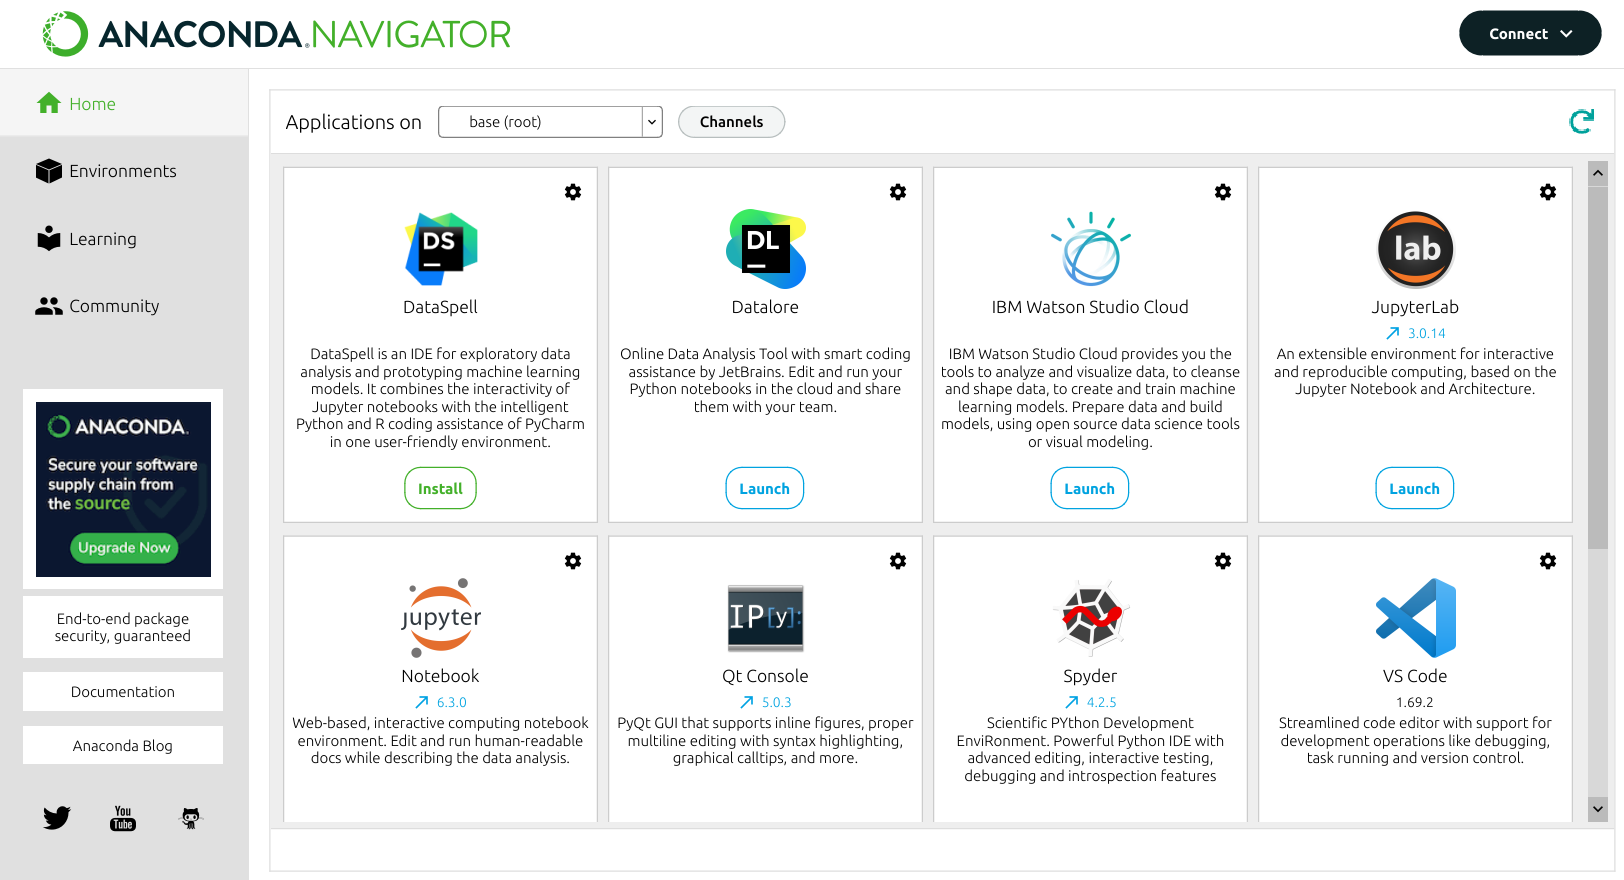
\includegraphics[width=1\textwidth]{anaconda_navigator}
	}
	\caption{A screenshot showing a sample of applications accessible from within Anaconda Navigator}
	\label{fig:anaconda_nav}
\end{sidewaysfigure}
\clearpage

\section{How Python Runs Programs}

\begin{paracol}{2}
	\question{Is Python a programming language or an interpreter?}
	\note{Short answer: BOTH. Typically, we refer to Python as a programming language. However, Python is also a software package called an interpreter, a kind of program that executes other programs. When you write a Python program, the Python interpreter reads your program and carries out the instructions it contains. In effect, the interpreter is a layer of software logic between your code and the computer hardware on your machine.
	}
\end{paracol}	

\begin{paracol}{2}
	\question{\raggedright How does an interpreter work?}
	\note{
	\begin{itemize}
		\item When you instruct Python to run your script (e.g., `script.py'), there are a few steps the interpreter carries out before your code starts crunching away (see Figure \ref{fig:python_interpreter})
		\item First, the code is compiled to something called `byte code'
		\begin{itemize}
			\item This step happens behind the scenes (there is nothing to do for the programmer!)
    			\item A file called `script.pyc', automatically generated, contains the translation of your code into lower-level code instructions
		\end{itemize}
		\item Then, the compiled code is routed to something called a `Python Virtual Machine' (PVM)
		\begin{itemize}
			\item This step is hidden to the programmer like the previous one
			\item Mainly, it iterates through your byte code instructions, one by one, to carry out their operations
		\end{itemize}
	\end{itemize}
	}
\end{paracol}

\begin{figure}[!htbp]
	\centering
	\sffamily
	\begin{tikzpicture}[
		->
	]
		\node [] (step) {\textbf{Step}};
	        \node [right=of step] (file) {\textbf{Entity}}; 
	        \node [below=of step] (source) {Source};
		\node [below=of file, align=right] (sourcef) {script.py};
		\node [below=of source] (byte) {Byte code};
		\node [below=of sourcef, align=right] (bytef) {script.pyc};
		\node [below=of byte] (pvm) {Runtime};
		\node [below=of bytef, align=right] (pvmf) {PVM};
		\path[]
			(source) edge node [] {} (byte)
			(byte) edge node [] {} (pvm);
	\end{tikzpicture}
	\caption{A stylized representation of Python's execution model}
	\label{fig:python_interpreter}
\end{figure}

\section{How We Run Python Programs}

\begin{paracol}{2}
	\question{\raggedright What are the alternative ways to run some Python code?}
	\note{There are two alternatives:
	\begin{itemize}
		\item The non-interactive way consists of preparing a Python script and running it from the command line
		\item The interactive way consist of preparing and running one or a few Python statements from within a Python shell 
	\end{itemize}
	}
\end{paracol}

\begin{paracol}{2}
	\question{\raggedright How do I run a Python script in the non-interactive way?}
	\note{One has to go through a two-step process:
	
	\begin{itemize}
		\item First, the script has to be prepared using a text editor (being basic or  sophisticated, it is up to you)
		\item Second, the script has be executed from the shel
	\end{itemize}

	\quad Snippet 1.1 shows a minimal Python script. Such a script can be created using the built-in text editor of your operating system or an advanced text editor such as \href{https://atom.io}{Atom}, \href{https://www.gnu.org/software/emacs/}{Emacs}, \href{https://www.gnu.org/software/emacs/}{Vim}/\href{https://neovim.io}{Neovim}, \href{https://www.sublimetext.com}{Sublime Text}, and \href{https://code.visualstudio.com}{Visual Studio Code}.

	\quad Once the script is saved to a file with extension \texttt{.py}, you can execute it from the command line by typing the following command in the shell session of our choice:

	\vspace{1em}

	\texttt{\$ python filename.py}

	\vspace{1em}

	\quad Let us unpack that command. The \texttt{\$} symbol denotes the
	statement has to be run in a shell session; the \texttt{python} command
	tells the shell to use the Python interpreter to evaluate the script;
	\texttt{filename.py} is the file name of the script. Figure
	\ref{fig:simple_script} shows how to run the Python script containing
	the code displayed in Snippet 1.1 (named \texttt{simple\_script.py}).
	\footnote{The example shown in the screenshot assumes the Python script
	\texttt{sample\_script.py} is saved in the current working directory. If
	the script is saved in a different directory, you have to specify the
	full path to the script in the command line.} It is self-evident the
	outcome of the script is displayed in the active shell session (we will
	see the \texttt{print} function in action many times over the next few
	chapters).
	}
	\end{paracol}

\begin{pythoncode}[linenos=True]{colback=base_c!5, colframe=base_c, title=\sffamily Snippet 1.1 --- a minimal Python script}
# Print a string object
print("Bazinga")

# Print the result of an algebraic operation
print(2 + 4)
\end{pythoncode}

\begin{figure}[!htbp]
	\begin{center}
		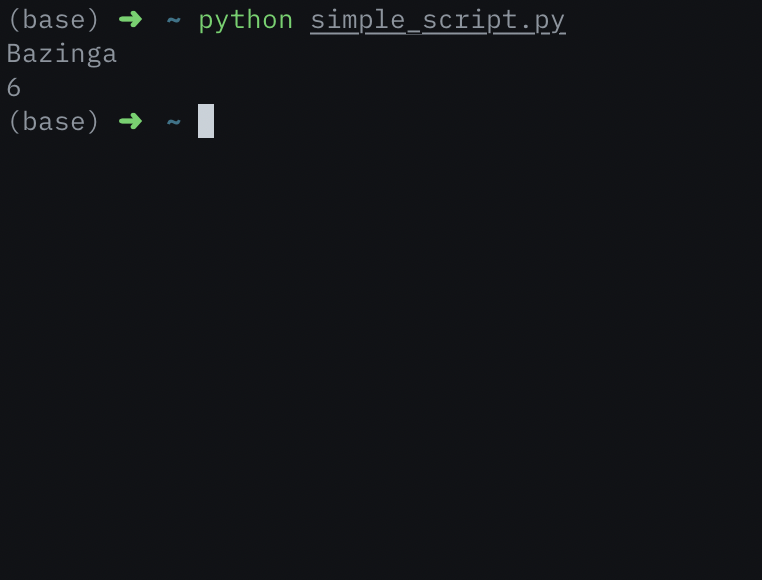
\includegraphics[width=0.5\textwidth]{simple_script}
	\end{center}
	\caption{A screenshot showing the execution of the minimal script included in Snippet 1.1}
	\label{fig:simple_script}
\end{figure}

\begin{paracol}{2}
	\question{\raggedright How do I interactively run a Python script?}
	\note{Mainly, there are three ways to do that:
	\begin{itemize}
		\item Running a Python shell in the terminal
		\item Running an IPython shell in the terminal
		\item Interacting with a Python or IPython shell through an Integrated Development Environment (IDE)
	\end{itemize}
	}
\end{paracol}

\begin{paracol}{2}
	\question{\raggedright How do I run Python code interactively using a Python or IPython shell?}
	\note{The first step is opening the terminal emulator of your choice (e.g., Windows Terminal, Cmder, Iterm, Terminator, Kitty). Then, you run the command \texttt{\$ python} or \texttt{\$ ipython} to start a Python and IPython shell respectively (see Figures \ref{fig:python_session} and \ref{fig:ipython_session}).
	}
\end{paracol}

\begin{figure}[!htbp]
	\centering
	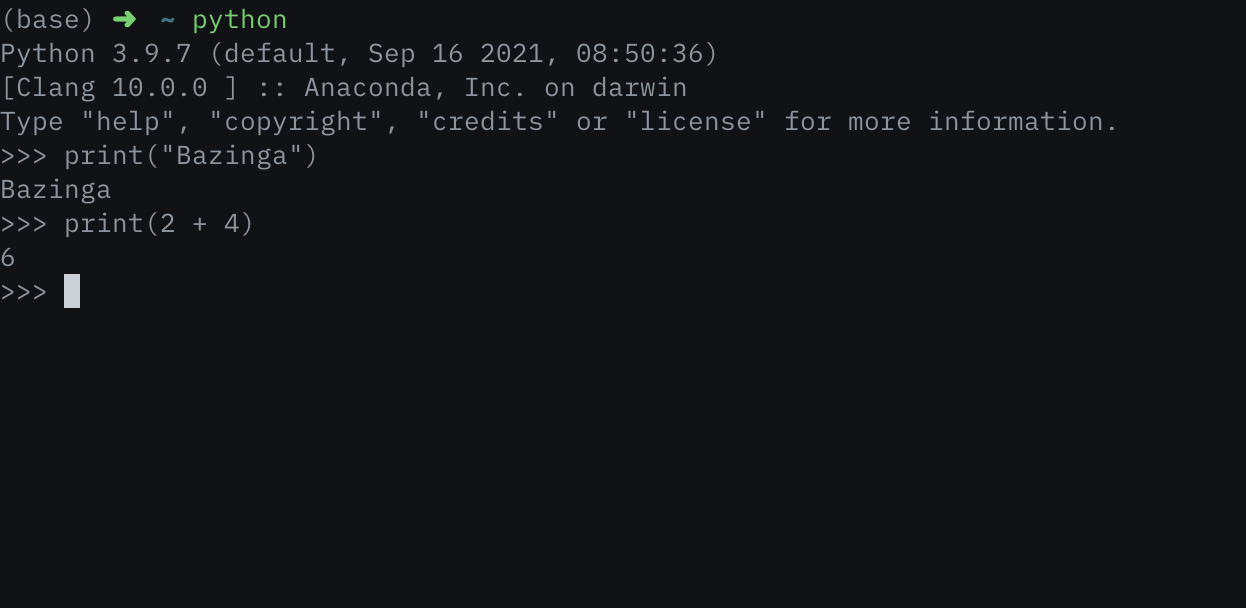
\includegraphics[width=0.75\textwidth]{python_session}
	\caption{A screenshot of an interactive Python shell}
	\label{fig:python_session}
\end{figure}
\clearpage

\begin{figure}[!htbp]
	\centering
	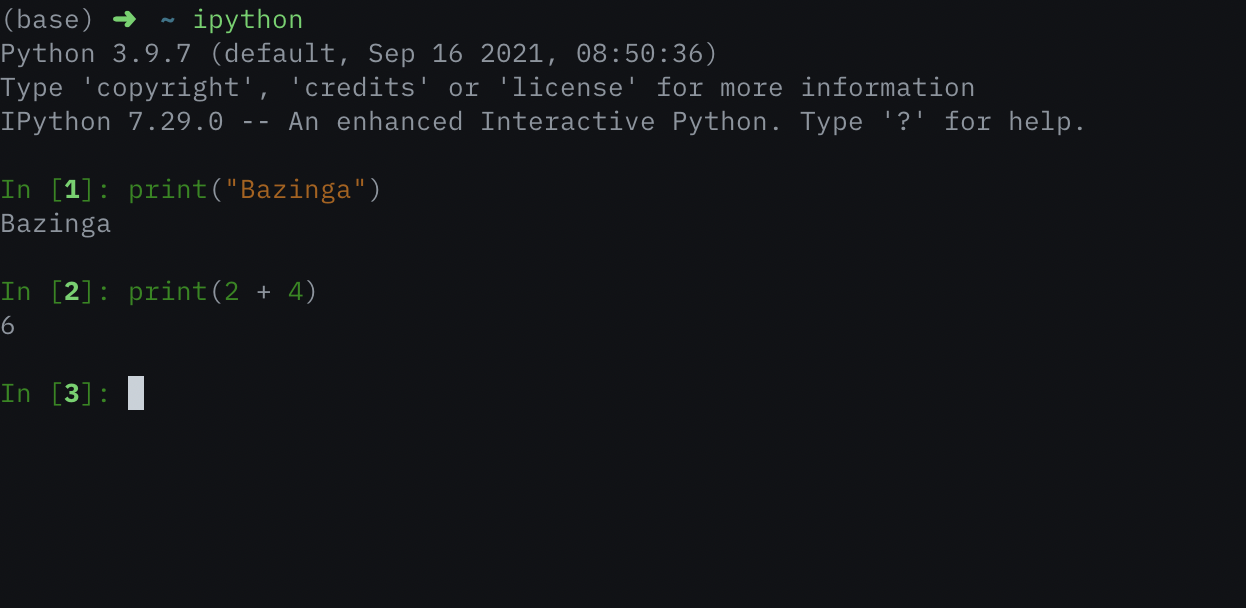
\includegraphics[width=0.75\textwidth]{ipython_session}
	\caption{A screenshot of an interactive IPython shell}
	\label{fig:ipython_session}
\end{figure}

\begin{paracol}{2}
	\question{\raggedright What are the most popular Python IDEs?}
	\note{There are plenty of Python IDEs in the market, including:
	
	\begin{itemize}
		\item Colab (online)
		\item IDLE
		\item Datalore (online)
		\item Jupyter/Jupyterlab 
		\item PyCharm
		\item Qt Console
		\item Spyder
		\item Thonny
		\item Wing
	\end{itemize}

	}
\end{paracol}

\begin{paracol}{2}
	\question{\raggedright Shall I start using Jupyter?}
	\note{Based on my experience, Jupyter sustains novices' programming learning in at least two ways. First, the graphical interface of a Jupyter notebook (see Figure \ref{fig:jupyter_session} allows learners to embrace a trial and error approach to coding by dissecting a script into manageable snippets --- or even single lines --- that can be better examined, understood, and tested. Second, the text boxes and rich media content typically included in a notebook provide learners with explanations to understand a script's logical structure and background.

	}
\end{paracol}
\clearpage

\begin{figure}[!htbp]
	\centering
	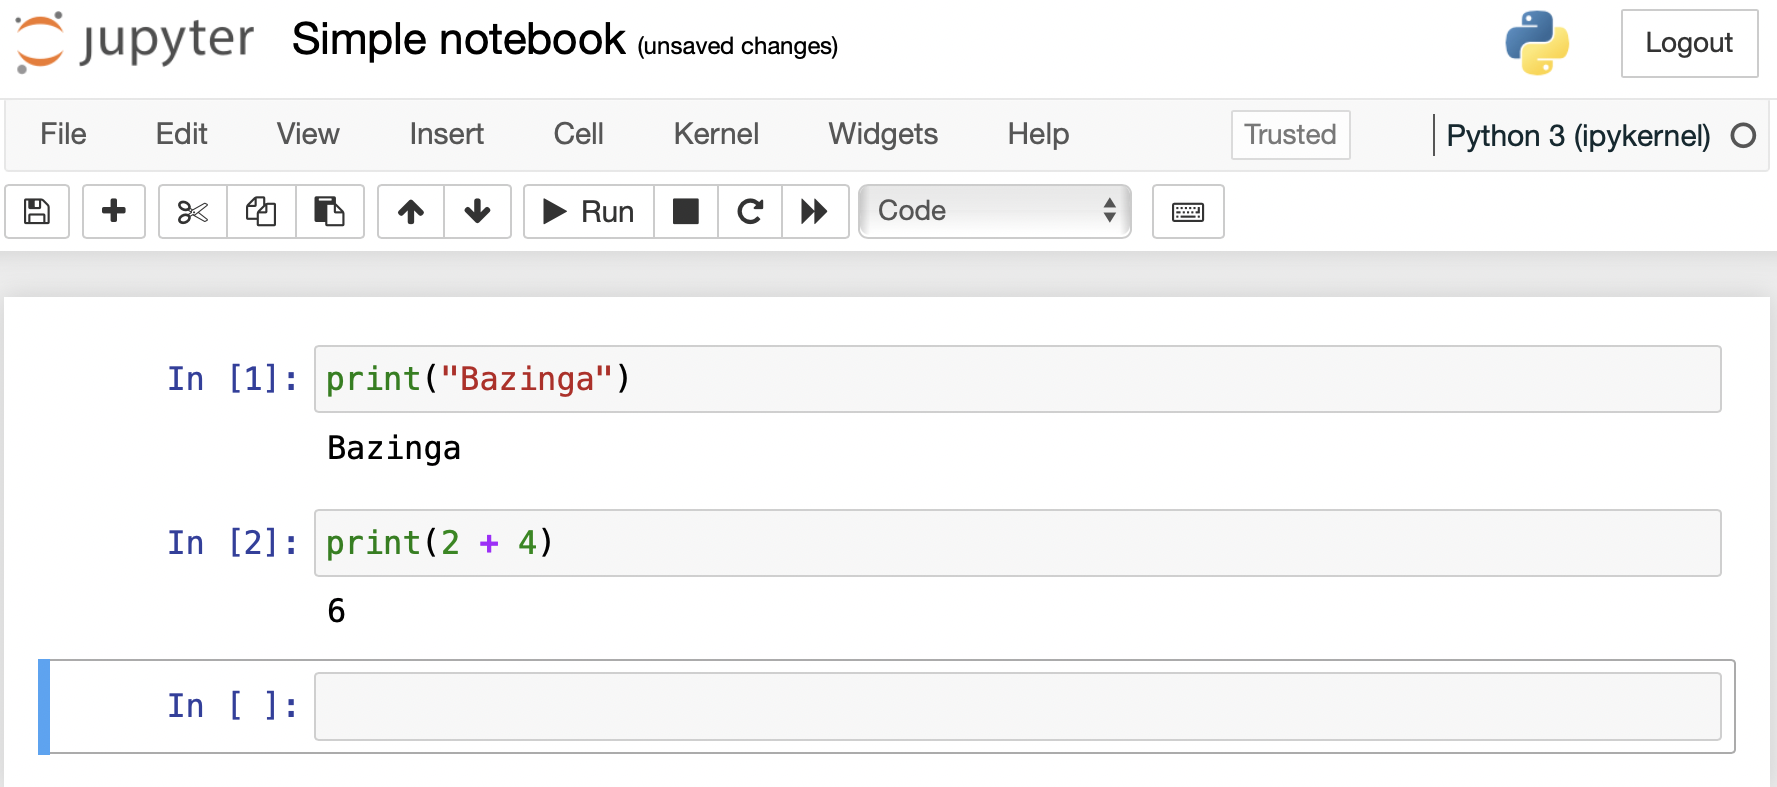
\includegraphics[width=0.8\textwidth]{jupyter}
	\caption{A screenshot of a Jupyter notebook session}
	\label{fig:jupyter_session}
\end{figure}	

\begin{paracol}{2}
	\question{\raggedright Can I turn an advanced text editor into a Python IDE?}
	\note{Of course. By installing a couple of plugins, the following (advanced) text editors can turn into Python IDEs
	
	\begin{itemize}
		\item Emacs 
		\item Vm/Neovim 
		\item Visual Studio Code (VSCode)
	\end{itemize}

	Figures \ref{fig:ipython_in_vscode} and \ref{fig:jupyter_in_vscode} show how to run an IPython and Jupyter session in VSCode respectively.\footnote{Please refer to the \href{https://code.visualstudio.com/docs/languages/python}{official documentation} on how to use Python in VSCode.}
	}
\end{paracol}	

\begin{figure}[!htbp]
	\centering
	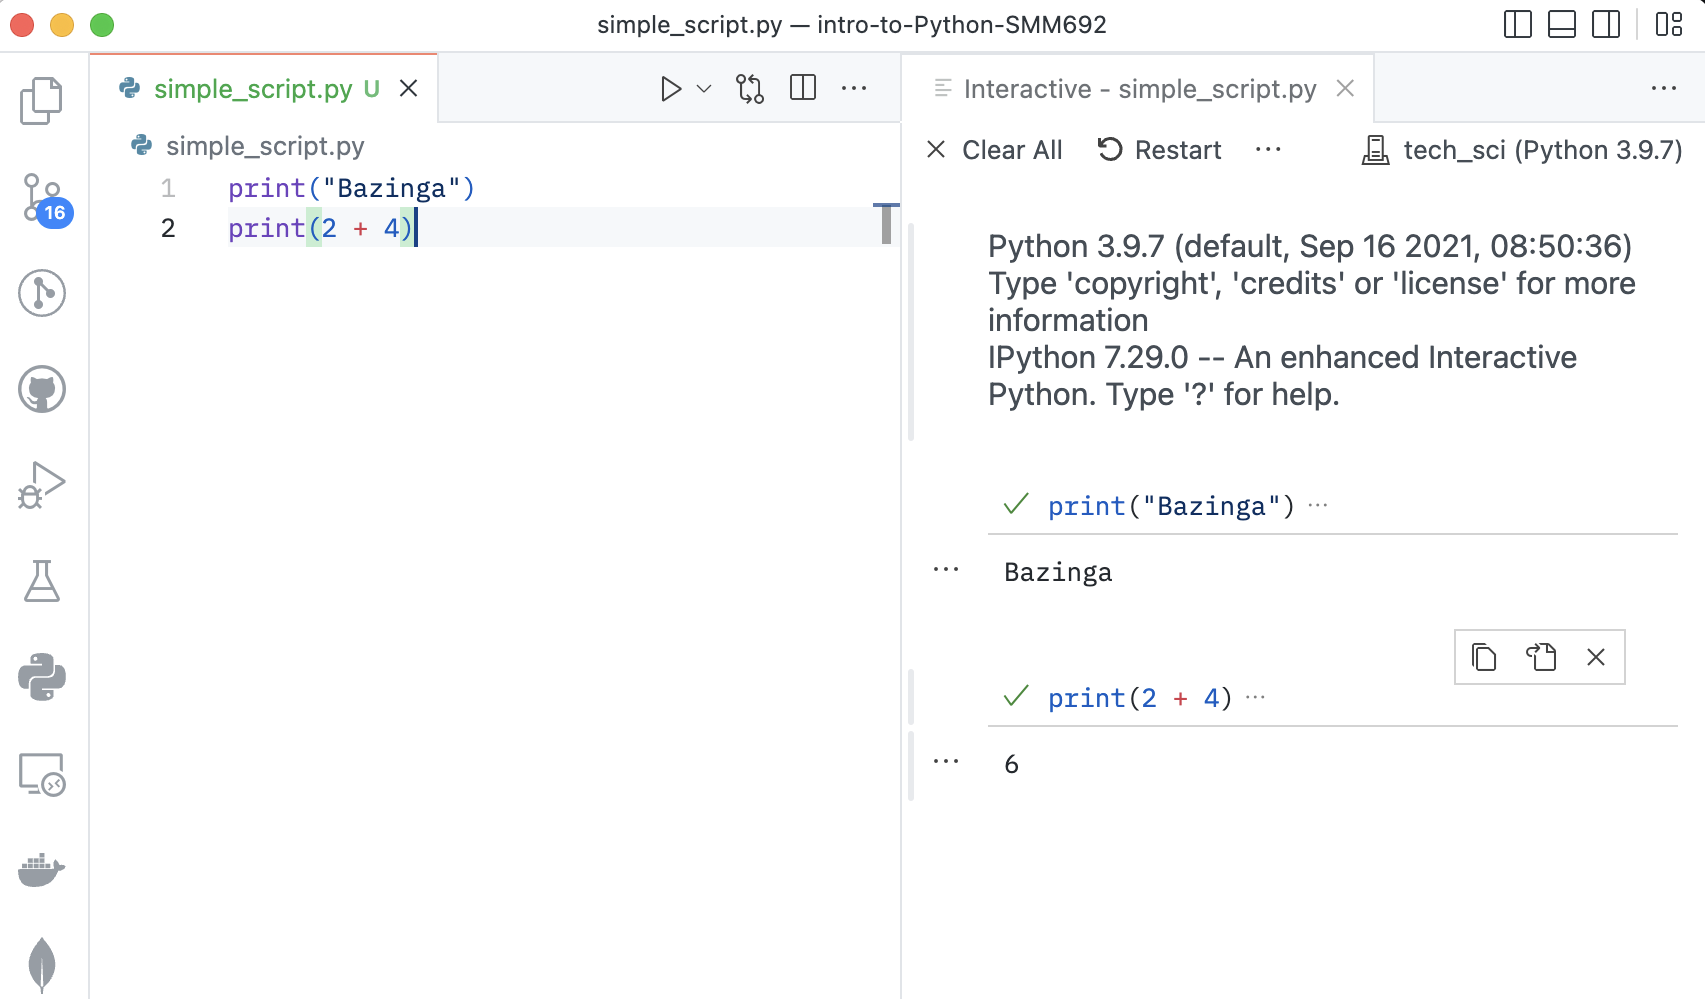
\includegraphics[width=0.95\textwidth]{vscode}
	\caption{A screenshot of an interactive IPython shell in VSCode}
	\label{fig:ipython_in_vscode}
\end{figure}	

\begin{figure}[!htbp]
	\centering
	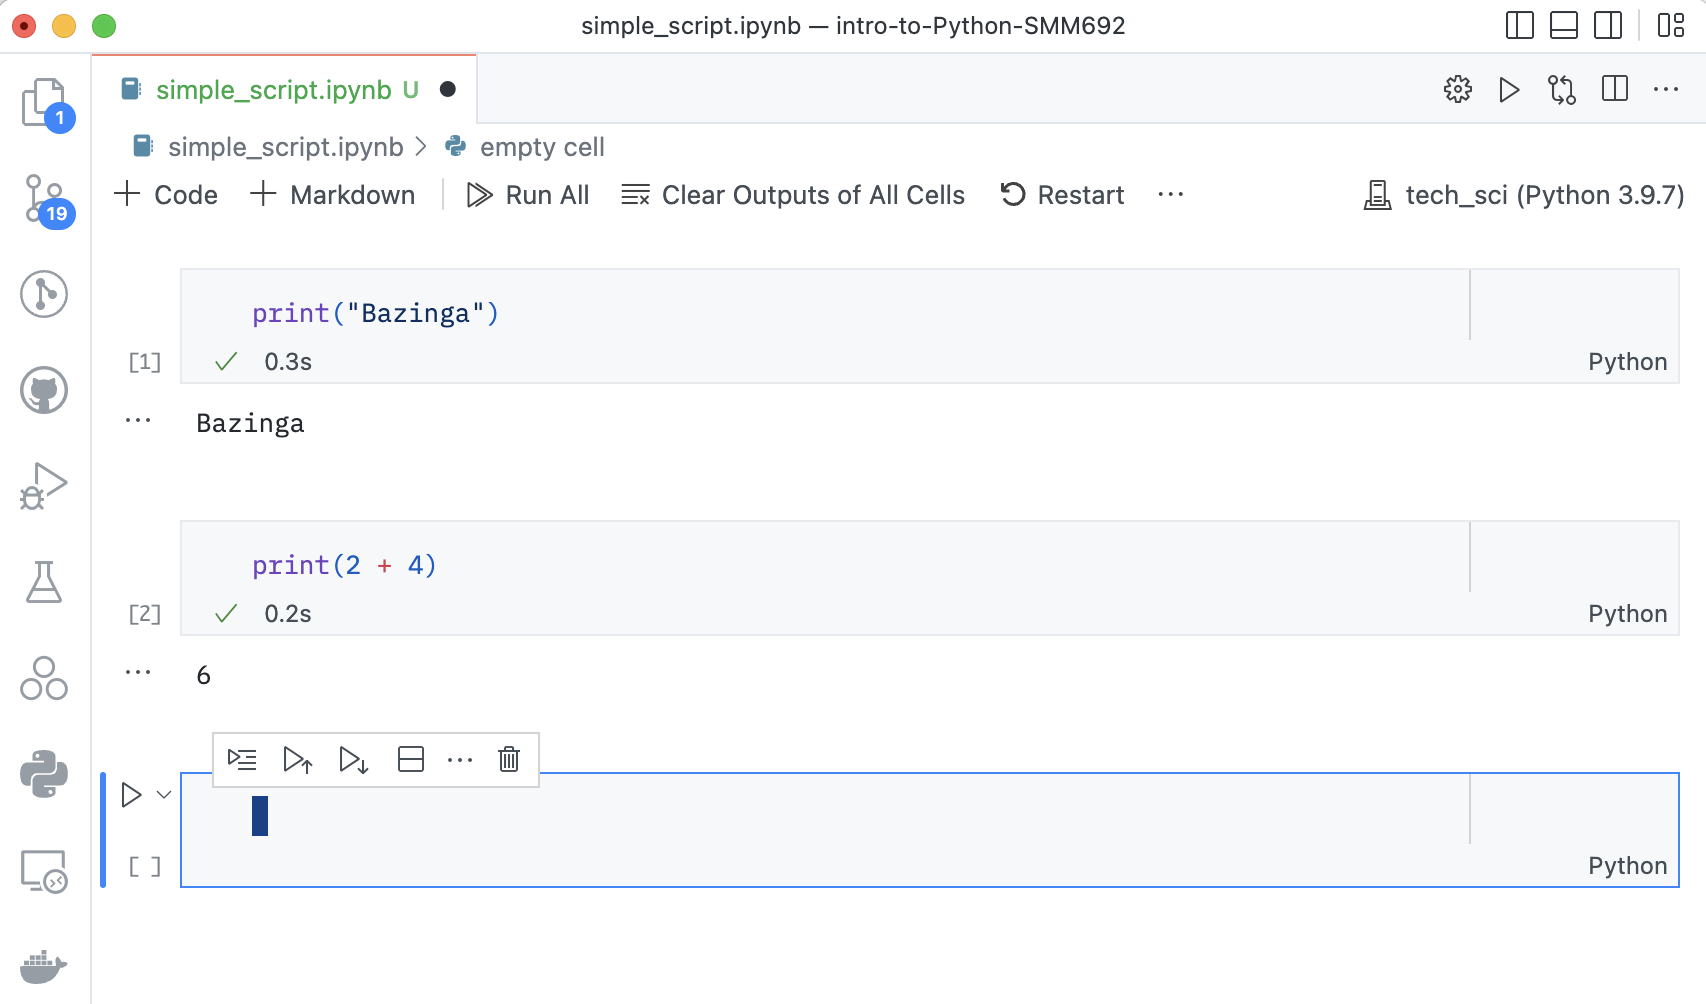
\includegraphics[width=0.95\textwidth]{jupyter_in_vscode}
	\caption{A screenshot of a Jupyter notebook session in VSCode}
	\label{fig:jupyter_in_vscode}
\end{figure}	
\clearpage

\section{Managing Python Environments}

\begin{paracol}{2}
	\question{\raggedright What is a Python environment?}
	\note{A Python environment is a self-contained directory that contains a Python interpreter, a set of Python packages, and their dependencies.
	}
\end{paracol}

\begin{paracol}{2}
	\question{\raggedright Why should I use a Python environment?}
	\note{Mainly, there are two reasons:
	\begin{enumerate}
		\item To protect the system-wise installation of Python
		\item To create collections of Python modules to deploy in specific projects/classes of projects (e.g., Machine Learning projects)
	\end{enumerate}
	}
\end{paracol}

\begin{paracol}{2}
	\question{\raggedright Why should I protect my system Python?}
	\note{
	The large majority of operating systems come with Python installed by default. Such an installation is called `system Python' and is responsible for many essential operating systems processes. 

	\quad Every time we install a new Python module $A$, the package manager (e.g, conda) checks the libraries on which $A$ depends. If a dependency $D(A)$ is not installed, the package manager will install it for us. The larger the number of libraries:
	\begin{itemize}
		\item The longer it takes to install a library (checking the web of dependencies takes substantial time!)
		\item The more likely inconsistencies will arise within the web of dependencies; that is
		\begin{itemize}
		\item The less likely we will be able to install the modules we need
		\item The more likely modules previously installed will stop work
		\end{itemize}
	\end{itemize}
	Ultimately, if you care about not breaking some essential features of the operating system, then you should avoid using `system Python' for projects requiring Python.
	}
\end{paracol}
\clearpage

\begin{paracol}{2}
	\question{\raggedright Why Python environments work well for specific projects?}
	\note{
	Typically, we create a Python environment to carry out a specific project or a class of projects (e.g., Machine Learning projects). The advantage is twofold:
	\begin{itemize}
		\item Reliability $\rightarrow$ the web of dependencies is relatively simple insofar as we install only the few modules that are required by the project or project class. Likely as not, we will not come across installation issues!
		\item Reproducibility $\rightarrow$ the environment explicates the modules are necessary to carry out a certain project. Hence, a user who wants to reproduce our project's results knows which modules to install
	\end{itemize}
	}
\end{paracol}

\begin{paracol}{2}
	\question{\raggedright How do I create a Python environment?}
	\note{
	The procedure to create a Python environment depends on the package
	manager you use (hence, the Python installation we have).  Here, I focus
	on the case where conda is the adopted package manager.\footnote{\texttt{pip} users are warmly encouraged to read the \href{https://docs.python.org/3/tutorial/venv.html}{Virtual Environments and Packages} section of the official Python Tutorial.}
	}
\end{paracol} 

\begin{paracol}{2}
	\question{\raggedright How do I use \texttt{conda} from the command line to create and populate a Python environment?}
	\note{
	To create a Python environment using \texttt{conda}, we can run the following command in the shell:
	
	\vspace{1em}

	\texttt{\$ conda create --name myenv python=3.X}

	\vspace{1em}

	where \texttt{conda} is the name of the package manager, \texttt{create}
	is the operation to run,\footnote{The
	\href{https://docs.conda.io/projects/conda/en/latest/commands.html}{Conda
	Command reference} illustrates the various commands Conda provides for
	managing packages and environments.} \texttt{myenv} is the name of the
	environment and \texttt{python=3.X} is the version of Python to use (e.g., 3.10).
	
	\quad To use the newly created environment, one has to activate it by running the following command in the shell:

	\vspace{1em}

	\texttt{\$ conda activate myenv}

	\vspace{1em}
	
	\quad At this point, one can install packages in the activated environment using the following command:

	\vspace{1em}

	\texttt{\$ conda install package\_name}

	\vspace{1em}

	\quad Figures \ref{fig:conda_env_cl_0} and \ref{fig:conda_env_cl_1} show a concrete example wherein a new Python environment is created and populated using \texttt{conda} from the command line.
	}
\end{paracol}

\begin{figure}[!htbp]
	\centering
	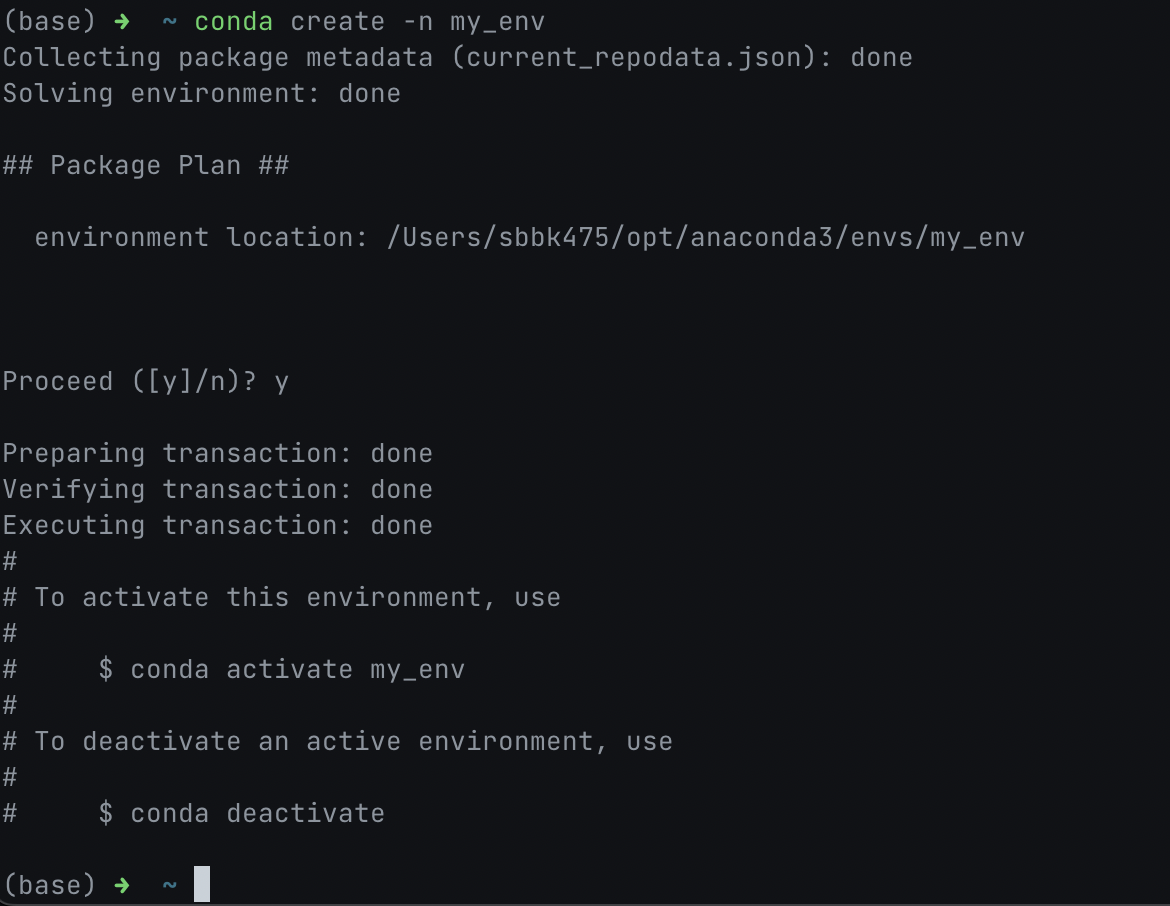
\includegraphics[width=0.70\textwidth]{conda_env_0}
	\caption{A screenshot showing how to create a Python environment using \texttt{conda} from the command line}
	\label{fig:conda_env_cl_0}
\end{figure}

\begin{figure}[!htbp]
	\centering
	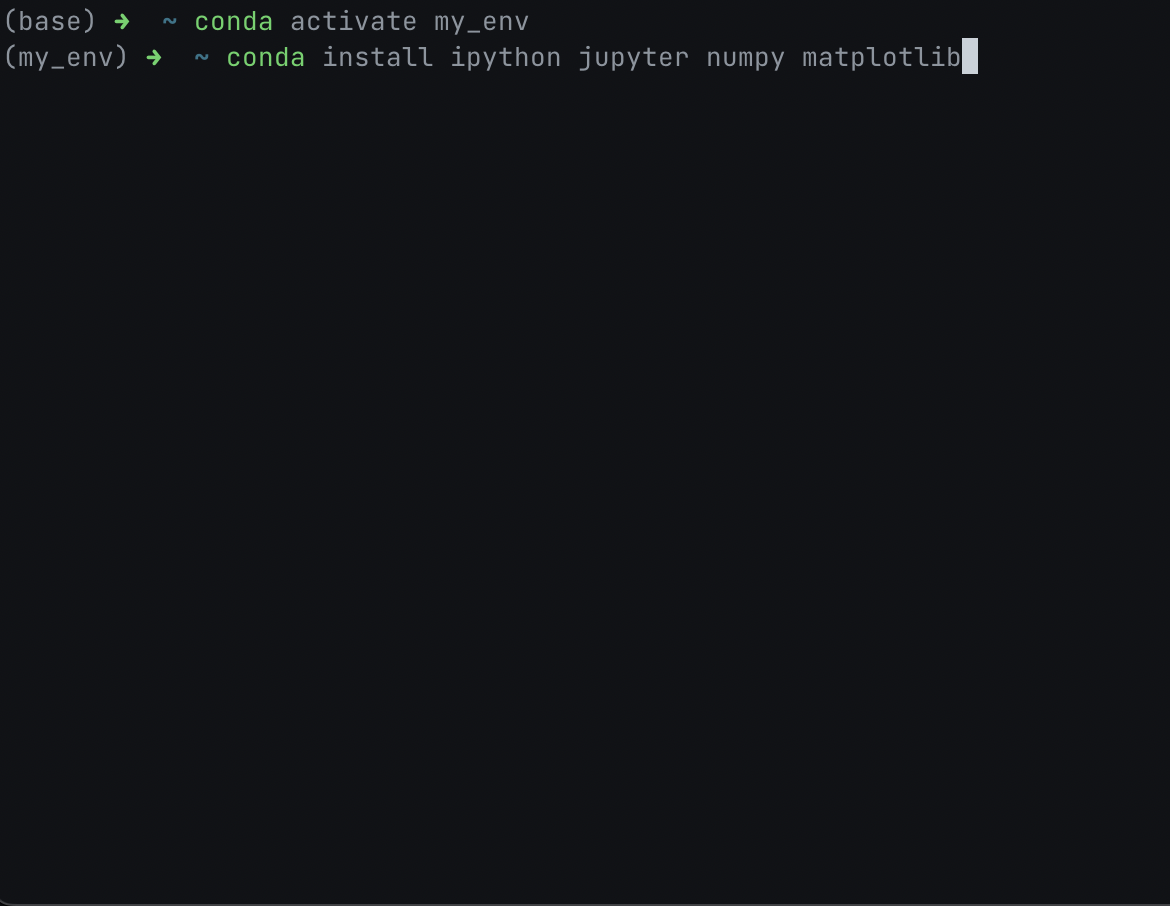
\includegraphics[width=0.75\textwidth]{conda_env_1}
	\caption{A screenshot showing how to populate a Python environment with libraries using \texttt{conda} from the command line}
	\label{fig:conda_env_cl_1}
\end{figure}
\clearpage

\begin{paracol}{2}
	\question{\raggedright How do I use Anaconda Navigator to create and populate a Python environment?}
	\note{
	\quad It is also possible to create a Python environment from within the Anaconda Navigator (Figures \ref{fig:anaconda_venv_0} and \ref{fig:anaconda_venv_1} provide a pictorial illustration of how to create a new environment and populate it with modules).
	}
\end{paracol}

\begin{sidewaysfigure}[!htbp]
	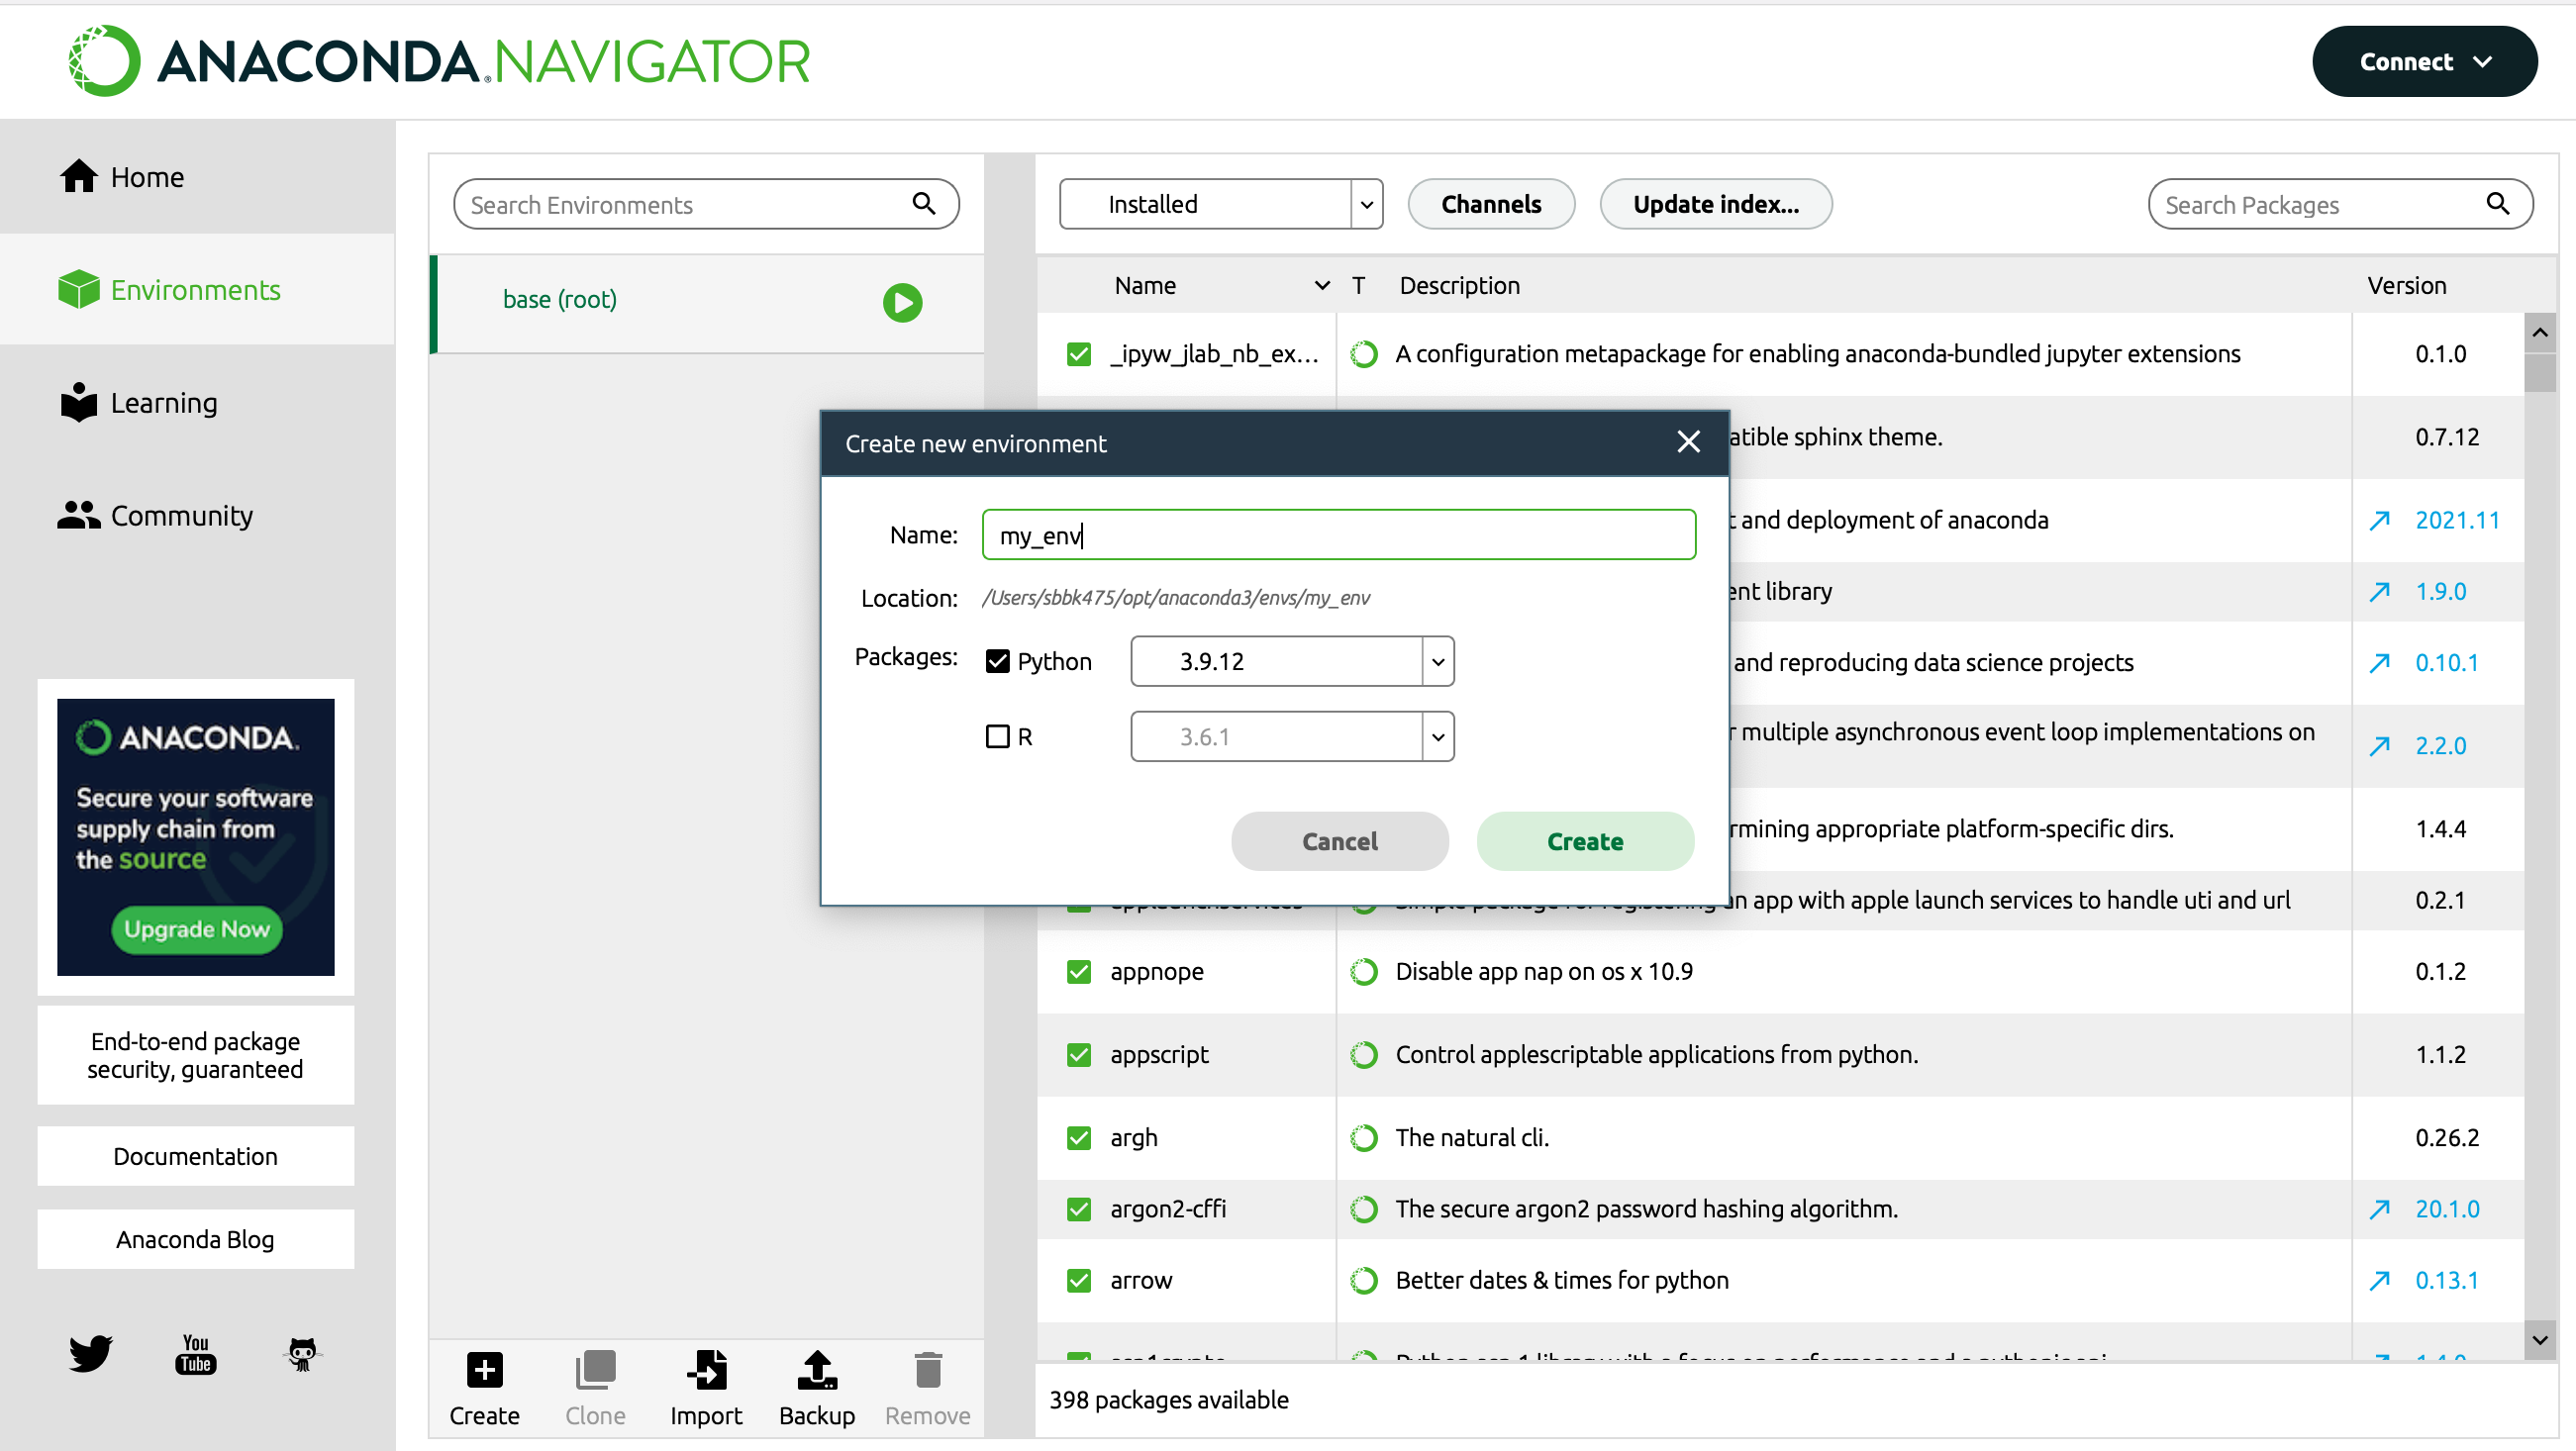
\includegraphics[width=1\textwidth]{anaconda_nav_env_0.png}
	\caption{A screenshot showing how to create a new environment from within the `Environments' section of Anaconda Navigator}
	\label{fig:anaconda_venv_0}
\end{sidewaysfigure}

\begin{sidewaysfigure}[!htbp]
	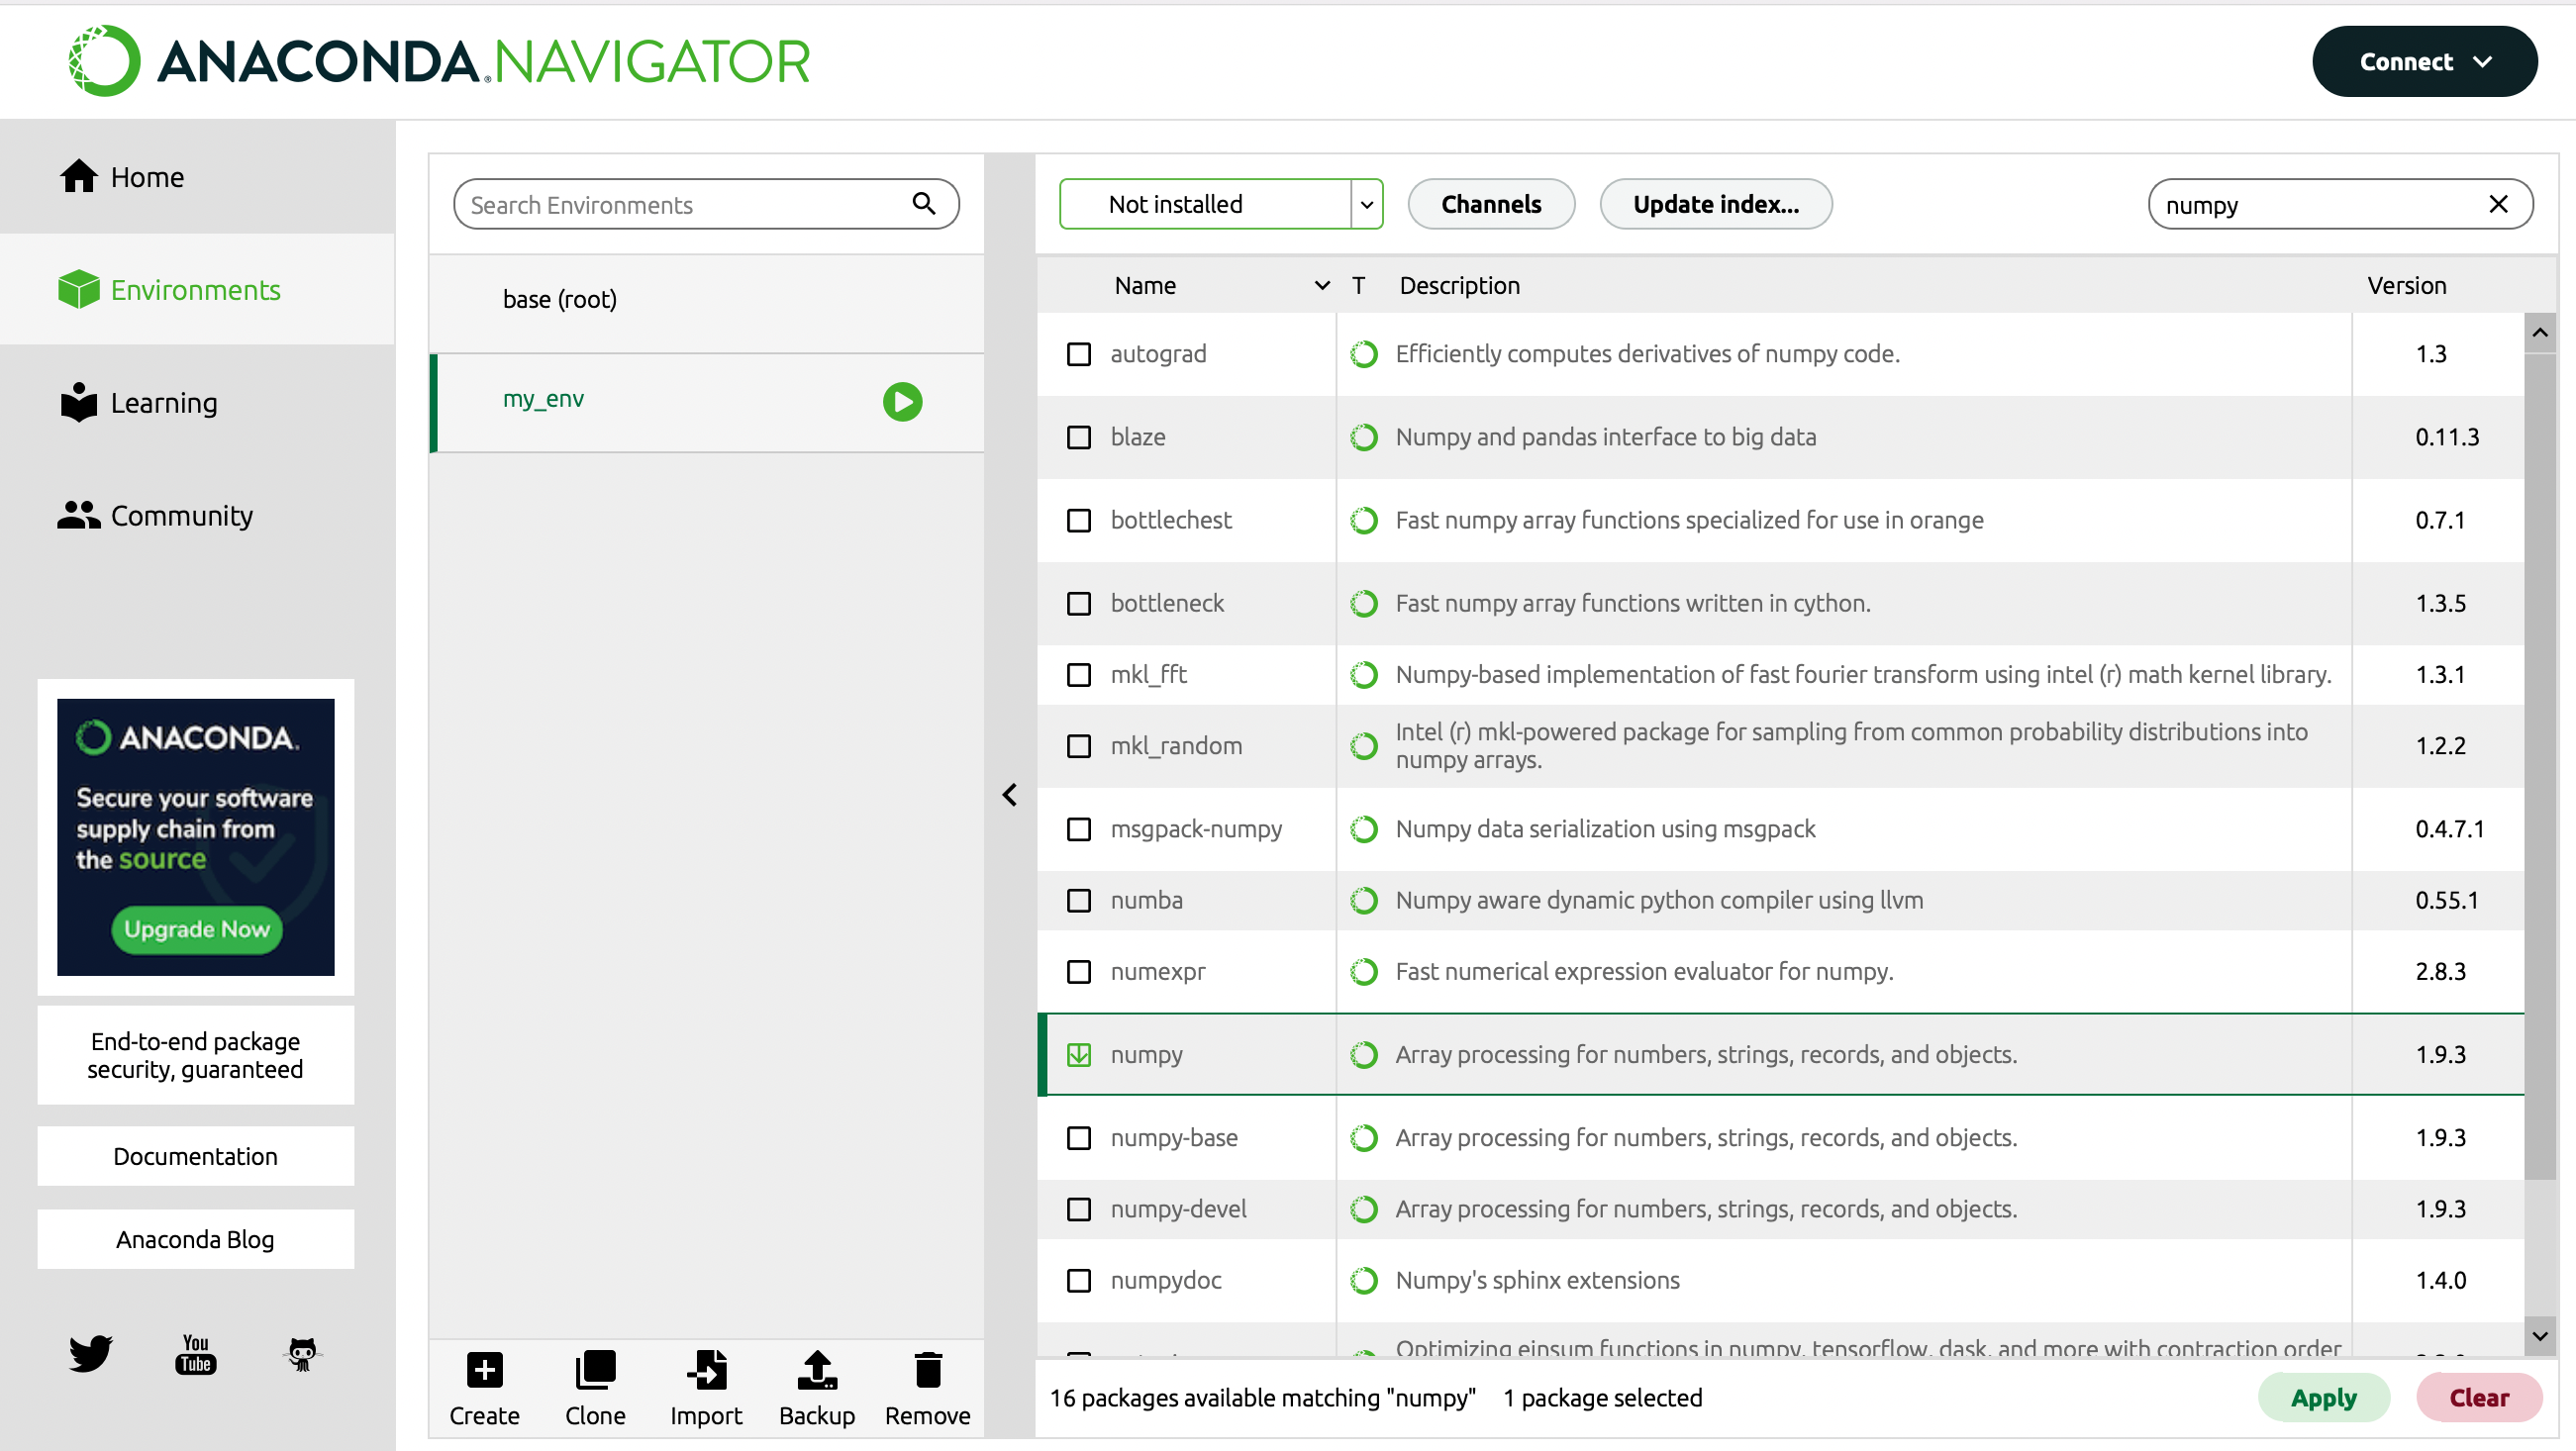
\includegraphics[width=1\textwidth]{anaconda_nav_env_1.png}
	\caption{A screenshot showing how to add Python modules to a (newly created) environment from within the `Environments' section of Anaconda Navigator}
	\label{fig:anaconda_venv_1}
\end{sidewaysfigure}
\clearpage

\theendnotes

\chapter{Python Objects}
\label{ch:objects}

\par\noindent\rule{\textwidth}{0.4pt}

At the end of the chapter, you will be able to evaluate the various types of Python objects in regard to:

\begin{itemize}
	\item Key features
	\item Use cases/roles
	\item Available methods
\end{itemize}

\par\noindent\rule{\textwidth}{0.4pt}

\vspace{1em}

\begin{paracol}{2}
    \question{\raggedright What is a Python object?} 
    \note{In essence, Python objects are pieces of data. Mark Lutz, the author of the popular book \href{https://www.google.co.uk/books/edition/Learning_Python/4pgQfXQvekcC?hl=en&gbpv=0}{Learning Python}\footnote{Lutz, Mark. \textit{Learning Python: Powerful object-oriented programming.} O'Reilly Media, Inc., 2013.}, points out \quote{``\textit{... in Python, we do things with stuff. ``Things'' take the form of operations like addition and concatenation, and ``stuff'' refers to the objects on which we perform those operations}''}. 
    }
\end{paracol}

\begin{paracol}{2}
    \question{\raggedright Built-in and ad-hoc objects}
    \note{In Python, there are two families of objects: built-in objects provided by the Python language itself and ad-hoc objects --- called \href{https://docs.python.org/3/tutorial/classes.html}{classes} --- we can create to accomplish specific goals.}
\end{paracol}
\clearpage

\begin{paracol}{2}
    \question{\raggedright Why do built-in Python objects matter?} 
    \note{
    Typically, we do not need to create ad-hoc objects. Python provides us with diverse built-in objects that make our job easier:
    \begin{itemize}
    	\item Built-in objects make coding efficient and easy. For example, using the \href{https://docs.python.org/3/tutorial/introduction.html\#strings}{string} object, we can represent and manipulate a piece of text --- e.g., a newspaper article --- without loading any \href{https://docs.python.org/3/tutorial/modules.html}{module}
    	\item Built-in objects are flexible. For example, we can deploy built-in objects to create a \href{https://docs.python.org/3/tutorial/classes.html}{class}
    	\item Built-in objects have been created and refined over time by a large community of expert developers. Hence, they are  often  more  efficient  than  ad-hoc objects (unless the creator of the ad-hoc object knows her business!)
    \end{itemize}
    }
\end{paracol}

\begin{paracol}{2}
    \question{\raggedright What are the core built-in Python objects?} 
	\note{Table \ref{tab:built_in_objects} illustrates the types of built-in Python objects. For example, \href{https://docs.python.org/3/tutorial/introduction.html\#numbers}{Numbers} and \href{https://docs.python.org/3/tutorial/introduction.html\#strings}{strings} objects are used to represent numeric and textual data respectively. \href{https://docs.python.org/3/tutorial/introduction.html\#lists}{Lists} and \href{https://docs.python.org/3/tutorial/datastructures.html\#dictionaries}{dictionaries} are --- likely as not --- the two most popular \href{https://docs.python.org/3/tutorial/datastructures.html}{data structures} in Python. Lists are ordered collections of other objects (any type!!). Dictionaries are pairs of keys (e.g., a product identifier) and objects (e.g., the product's price). No worries: we will go through each built-in type in the following sections of this document. Caveat: in the interest of logical coherence, the various built-in types will not be presented in the order adopted in Table \ref{tab:built_in_objects}.} 
\end{paracol}

\begin{table}[!htbp]
\centering
\caption{Built-In Objects in Python}
\label{tab:built_in_objects}
\begin{tabular}{@{}ll@{}}
\toprule \toprule
Object type          & Example literals/creation                                            \\ \midrule
Numbers              & 1234, 3.1415, 3+4j, 0b111, Decimal(), Fraction()                     \\
Strings              & `spam', ``Bob's'', b`a\textbackslash{}x01c', u`sp\textbackslash{}xc4m' \\
Lists                & {[}1, {[}2, `three'{]}, 4.5{]}, list(range(10))                      \\
Dictionaries         & \{`food': `spam', `taste': `yum'\}, dict(hours=10)                   \\
Tuples               & (1, `spam', 4, `U'), tuple(`spam'), namedtuple                       \\
Files                & open(`eggs.txt'), open(r`C:\textbackslash{}ham.bin', `wb')           \\
Sets                 & set(`abc'), \{`a', `b', `c'\}                                        \\
Other core types     & Booleans, types, None                                                \\
Program unit types   & Functions, modules, classes                                          \\
Implementation types & Compiled code, stack tracebacks                                      \\ \bottomrule
\end{tabular}
\end{table}
\clearpage

\section{Number Type Fundamentals}

\begin{paracol}{2}
    \question{\raggedright What are the types of `number' objects?}
	\note{Snippet 4.1, ``Doing stuff with numbers,'' highlights the two most popular \href{https://docs.python.org/3/tutorial/introduction.html\#numbers}{`number'} instances in Python: integers and floating-point numbers. Integers are whole numbers such as 0, 4, or -12. Floating-point numbers represent real numbers such as 0.5, 3.1415, or -1.6e-19. However, floating points in Python do not have --- in general --- the same value as the real number they represent.\footnote{Floating numbers are stored in binaries with an assigned level of precision typically equivalent to 15 or 16 decimals.} It is worth noticing that any single number with a period `.' is considered a floating point in Python. Also, Snippet 4.1 shows that the multiplication of an integer by a floating point yields a floating point. That happens because Python first converts operands to the type of the most complicated operand.} 
\end{paracol}

\begin{pythoncode}[linenos=true,]{colback=base_c!5, colframe=base_c, title=\sffamily Snippet 4.1 --- doing `stuff' with numbers}
# integer addition
>>> 1 + 1
2

# floating-point multiplication
>>> 10 * 0.5
5.0

# 3 to the power 100
>>> 3 ** 100
515377520732011331036461129765621272702107522001

\end{pythoncode}

\begin{paracol}{2}
	\question{\raggedright Are there any other number types besides integers and floating points?}
    \note{Besides integers and floating points numbers, Python includes fixed-precision, rational numbers, Booleans, and sets instances --- see Table \ref{tab:number_types_in_python}.}
\end{paracol}

\begin{table}[!htbp]
	\centering
	\caption{Number Type Objects in Python}
	\label{tab:number_types_in_python}
	\begin{tabular}{ll}
		\toprule \toprule
		Literal & Interpretation\\
		\midrule
		 1234, -24, 0, 99999999999999 & Integers (unlimited size)\\
		 1.23, 1., 3.14e-10, 4E210, 4.0e+210 & Floating-point numbers \\
		 0o177, 0x9ff, 0b101010 & Octal, hex, and binary literals in 3.X \\
		 0177, 0o177, 0x9ff, 0b101010 & Octal, octal, hex, and binary literals in 2.X \\
		 3+4j, 3.0+4.0j, 3J & Complex number literals \\
		 set(`spam'), \{1, 2, 3, 4\} & Sets: 2.X and 3.X construction forms\\ Decimal(`1.0'), Fraction(1, 3) & Decimal and fraction extension types\\
		 bool(X), True, False & Boolean type and constants\\
		 \bottomrule
	\end{tabular}
\end{table}
\clearpage

\begin{paracol}{2}
	\question{\raggedright How do I carry out basic arithmetic operations in Python?}
	\note{Numbers in Python support the usual mathematical operations:
		\begin{itemize}
			\item \texttt{+} $\rightarrow$ addition
			\item \texttt{-} $\rightarrow$ subtraction
			\item \texttt{*} $\rightarrow$ multiplication
			\item \texttt{$\setminus$} $\rightarrow$ floating point division
			\item \texttt{//} $\rightarrow$ integer division
			\item \texttt{\%} $\rightarrow$ modulus (remainder)
			\item \texttt{**} $\rightarrow$ exponentiation
		\end{itemize}
		 To use these operations, it is sufficient to launch a  Python or IPython session without any modules loaded (see Snippet 4.1).}
\end{paracol}

\begin{paracol}{2}
    \question{\raggedright How do I carry out advanced mathematical operations?}
    \note{Besides the mathematical operations shown above, there are many \href{https://docs.python.org/3/library/numeric.html}{modules shipped with Python} that carry out advanced/specific numerical analysis. For example, the \href{https://docs.python.org/3/library/math.html}{\texttt{math}} module provides access to the mathematical functions defined by the \href{https://en.wikipedia.org/wiki/C_standard_library}{C standard}.\footnote{As per the documentation of the Python programming language, \href{https://docs.python.org/3/library/math.html}{\texttt{math}} cannot be used with complex numbers.} Table \ref{tab:math_module_functions} reports a sample of these functions. To use them \href{https://docs.python.org/3/library/math.html}{\texttt{math}}, we have to import the module as shown in Snippet 4.2. Another popular module shipped with Python is \href{https://docs.python.org/3/library/random.html}{\texttt{random}}, implementing pseudo-random number generators for various distributions (see the lower section of Example 2).}
\end{paracol}

\begin{table}[!htbp]
	\centering
	\caption{A Sample of Functions Provided by the \href{https://docs.python.org/3/library/math.html}{\texttt{math}} Module}
	\label{tab:math_module_functions}
	\begin{tabular}{ll}
		\toprule \toprule
		Function name &  Expression \\
		\midrule
		\texttt{math.sqrt(x)} & $\sqrt{x}$ \\
		\texttt{math.exp(x)} & $e^{x}$ \\
		\texttt{math.log(x)} & $ln{x}$ \\
		\texttt{math.log(x, b)} & $log_{b}(x)$ \\
		\texttt{math.log10(x)} & $log_{10}(x)$ \\
		\texttt{math.sin(x)} & $sin(x)$ \\
		\texttt{math.cos(x)} & $cos(x)$ \\
		\texttt{math.tan(x)} & $tan(x)$ \\
		\texttt{math.asin(x)} & $arcsin(x)$ \\
		\texttt{math.acos(x)} & $arccos(x)$ \\
		\texttt{math.atan(x)} & $arctan(x)$ \\
		\texttt{math.sinh(x)} & $sinh(x)$ \\
		\texttt{math.cosh(x)} & $cosh(x)$ \\
		\texttt{math.tanh(x)} & $tanh(x)$ \\
		\texttt{math.asinh(x)} & $arsinh(x)$ \\
		\texttt{math.acosh(x)} & $arcosh(x)$ \\
		\texttt{math.atanh(x)} & $artanh(x)$ \\
		\texttt{math.hypot(x, y)} & The Euclidean norm, $\sqrt{x^{2} + y^{2}}$ \\
		\texttt{math.factorial(x)} & $x!$ \\
		\texttt{math.erf(x)} & The error function at $x$ \\
		\texttt{math.gamma(x)} & The gamma function at $x$, $\omega(x)$ \\
		\texttt{math.degrees(x)} & Converts $x$ from radians to degrees \\
		\texttt{math.radians(x)} & Converts $x$ from degrees to radians\\
		\bottomrule 
	\end{tabular}
\end{table}
\clearpage

\begin{pythoncode}[linenos=true,]{colback=base_c!5, colframe=base_c, title=\sffamily Snippet 4.2 --- advanced mathematical operations with the math module}
# import the math module
>>> import math
	
# base-y log of x
>>> math.log(12, 8)
1.1949875002403856
	
# base-10 log of x
>>> math.log10(12)
1.0791812460476249
	
# import the random module
>>> import random
	
# a draw from a normal distribution with mean = 0 and standard deviation = 1
>>> random.normalvariate(0, 1)
-0.136017752991189

# trigonometric functions
>>> math.cos(0)
1.0

>>> math.sin(0)
0.0

>>> math.tan(0) 
0.0

# an expression containing a factorial product
>>> math.factorial(4) - 4 * 3 * 2 * 1
0
\end{pythoncode}

\begin{paracol}{2}
	\question{What is the precedence order among Python operators?}
    \note{As shown in Snippet 4.2, line 30, Python expressions can string together multiple operators. So, how does Python know which operation to perform first? The answer to this question lies in operator precedence. When you write an expression with more than one operator, Python groups its parts according to what is called precedence rules,\footnote{The official Python documentation has an extensive section on operator precedence rules in the section dedicated to \href{https://docs.python.org/3/reference/expressions.html}{syntax of expressions}} and this grouping determines the order in which the expression’s parts are computed. Table \ref{tab:operator_precedence} reports the precedence hierarchy concerning the most common operators. Note that operators lower in the table have higher precedence. Parentheses can be used to create sub-expressions that override operator precedence rules.}
\end{paracol}
\clearpage

\begin{table}[!htbp]
	\centering
	\caption{Operator Precedence Hierarchy \\(Ascending Order)}
	\label{tab:operator_precedence}
	\begin{tabular}{ll}
		\toprule \toprule
        Operator & Description\\ 
        \midrule
        \texttt{x + y}    & Addition, concatenation \\
        \texttt{x - y}    & Subtraction, set difference \\
        \texttt{x * y}    & Multiplication, repetition \\ 
        \texttt{x \% y}   & Remainder, format; \\
        \texttt{x / y}, \texttt{x // y} & Division: true and floor \\
        \texttt{-x}, \texttt{+x} & Negation, identity \\
        \texttt{$^{\sim}$x}       & Bitwise NOT (inversion) \\
        \texttt{x ** y}  & Power (exponentiation) \\
        \bottomrule
    \end{tabular}
\end{table}

\begin{paracol}{2}
	\question{\raggedright How do I carry out technical and scientific computation with Python?}
	\note{Python is at the center of a rich ecosystem of modules for technical and scientific computation. In the following chapter, the attention will revolve around one of the most prominent modules, namely, \href{https://numpy.org/}{NumPy}. In a nutshell, \href{https://numpy.org/}{NumPy} offers the infrastructure for efficiently manipulating data structures. \href{https://scipy.org/}{SciPy} builds on \href{https://numpy.org/}{NumPy} to implement many algorithms across the fields of statistics, linear algebra, optimization, calculus, signal processing,  image processing, and others. Another core module in the technical and scientific domain is \href{https://www.sympy.org/en/index.html}efficiently manipulatingSimPy}, a library for symbolic mathematics. Note that none of these three modules are shipped with Python and should be installed with the package manager of your choice (e.g., \texttt{conda}).}
\end{paracol}
\clearpage

\begin{paracol}{2}
	\question{\raggedright What is a Python variable?}
	\note{Variables are simply names --- created by you or Python --- that are used to keep track of information in your program. In Python:
	\begin{itemize}
		\item Variables are created when they are first assigned values
		\item Variables are replaced with their values when used in expressions
		\item Variables must be assigned before they can be used in expressions
		\item Variables refer to objects and are never declared ahead of time
	\end{itemize}
    As Snippet 4.3 shows, the assignment of \texttt{x = 2} causes the variable \texttt{x} to come into existence `automatically.' From that point, we can use the variables in the context of expressions such as the ones displayed in lines 8, 12, 16, and 20 or create new variables like in line 24.
    }
\end{paracol}

\begin{pythoncode}[linenos=true,]{colback=base_c!5, colframe=base_c, title=\sffamily Snippet 4.3 --- expressions involving arithmetic operations}
	
# let us assign the variables 'x' and 'y' to two number objects
>>> x = 2

>>> y = 4.0	

# subtracting an integer from variable 'x'
>>> x - 1
1

# dividing the variable 'y' by an integer
>>> y / 73
0.0547945205479452

# integer-dividing the variable 'y' by an integer
>>> y // 73
0.0

# getting a linear combination of 'x' and 'y'
>>> 3 * x - 5 * y
-14.0

# assigning the variable 'z' to the linear combination of 'x' and 'y'
>>> z = 3 * x - 5 * y

\end{pythoncode}
\clearpage

\begin{paracol}{2}
	\question{\raggedright How do I display number objects in a readable way?}
	\note{Snippet 4.3 includes some expressions whose result is not passed to a new variable (e.g., lines 8, 12, 16, 20). In those cases, the IPython session displays the outcome of the expression `as is (e.g., 0.0547945205479452). However, a number with more than three or four decimals may not suit the table or report we must prepare. Python has powerful \href{https://docs.python.org/3/library/string.html}{string formatting} capabilities to display number objects in a readable and nice manner. Table \ref{tab:number_formatting} illustrates various number formatting options with concrete cases. Format strings contain `replacement fields' surrounded by curly braces \texttt{\{\}}. Anything that is not contained in braces is considered literal text, which is copied unchanged to the output. Snippet 4.4 presents a fully-fledged number formatting case. First, we assign the variable \texttt{a} to a floating-point number (line 2). Then, we pass the formatting option \texttt{\{:.2f\}} over the variable \texttt{a} using the Python built-in function \href{https://docs.python.org/3/library/stdtypes.html\#str.format}{\texttt{format}}.}
\end{paracol}

\begin{table}[!htbp]
	\centering
	\caption{Number Formatting Options in Python}
	\label{tab:number_formatting}
	\begin{tabular}{cccll}
		\toprule \toprule
		\multicolumn{1}{c}{Number} &
		\multicolumn{1}{c}{Format} & 
		\multicolumn{1}{c}{Output} & 
		\multicolumn{1}{c}{Description} \\
		\midrule
		3.1415926                           & \texttt{\{:.2f\}}                            & 3.14                                & Format float 2 decimal places                 &  \\
		3.1415926                           & \texttt{\{:+.2f\}}                           & +3.14                               & Format float 2 decimal places with sign       &  \\
		-1                                  & \texttt{\{:+.2f\}}                           & -1.00                               & Format float 2 decimal places with sign       &  \\
		2.71828                             & \texttt{\{:.0f\}}                            & 3                                   & Format float with no decimal places           &  \\
		5                                   & \texttt{\{:0\textgreater{}2d\}}              & 05                                  & Pad number with zeros (left padding, width 2) &  \\
		5                                   & \texttt{\{:x\textless{}4d\}}                 & 5xxx                                & Pad number with x’s (right padding, width 4)  &  \\
		10                                  & \texttt{\{:x\textless{}4d\}}                 & 10xx                                & Pad number with x’s (right padding, width 4)  &  \\
		1000000                             & \texttt{\{:,\}}                              & 1,000,000                           & Number format with comma separator            &  \\
		0.25                                & \texttt{\{:.2\%\}}                           & 25.00\%                             & Format percentage                             &  \\
		1000000000                          & \texttt{\{:.2e\}}                            & 1.00e+09                            & Exponent notation                             &  \\
		13                                  & \texttt{\{:10d\}}                            & \multicolumn{1}{r}{13}              & Right aligned (default, width 10)             &  \\
		13                                  & \texttt{\{:\textless{}10d\}}                 & \multicolumn{1}{l}{13}              & Left aligned (width 10)                       &  \\
		13                                  & \texttt{\{:\textasciicircum{}10d\}}          & 13                                  & Center aligned (width 10)                     \\
		\bottomrule
	\end{tabular}
\end{table}

\begin{pythoncode}[linenos=true,]{colback=base_c!5, colframe=base_c, title=\sffamily Snippet 4.4 --- number formatting in Python}
# assign the variable 'a' to a floating-point number
>>> a = 0.67544908755

# displaying 'a' with the first two decimals only
>>> "{:.2f}".format(a)
"0.68"

# displaying 'a' with the first three decimals only
>>> "{:.3f}".format(a)
"0.675"
\end{pythoncode}

\begin{paracol}{2}
	\question{\raggedright{How do I compare number objects?}}
	\note{Comparisons are used frequently to create control \href{https://docs.python.org/3/tutorial/controlflow.html}{flows}, a topic we will discuss later in this chapter. Normal comparisons in Python regard two number objects and return a Boolean result. Chained comparisons concern three or more objects and, like normal comparisons, yield a Boolean result. Snippet 4.5 provides a sample of normal comparisons (between lines 1 and 15) and chained comparisons (between lines 21 and 30). As evident in the example, comparisons can regard both numbers and variables assigned to numbers. Chained comparisons can take the form of a range test (see line 21), a joined, `AND' test of the truth of multiple expressions (see line 25), or a disjoined, `OR' test of the truth of multiple expressions (see line 29).}
\end{paracol}

\begin{pythoncode}[linenos=true,]{colback=base_c!5, colframe=base_c, title=\sffamily Snippet 4.5 --- comparing numeric objects}
# less than
>>> 3 < 2
False

# greater than or equal
>>> 1 <= 2
True

# equal
>>> 2 == 2
True 

# not equal
>>> 4 != 4
False

# range test
>>> x = 3
>>> y = 5
>>> z = 4
>>> x < y < z
False

# joined test
>>> x < y and y > z
True

# disjoined test
>>> x < y or y < z
True 

\end{pythoncode}
\clearpage

\section{String Type Fundamentals}

\begin{paracol}{2}
	\question{What is a string?}
	\note{A Python string is a positionally ordered collection of other objects. Sequences maintain a left-to-right order among the items they contain: their items are stored and fetched by their relative positions. Strictly speaking, strings are \textit{immutable sequences} of one-character strings; other, more general sequence types include lists and tuples, covered later.}
\end{paracol}

\begin{paracol}{2}
	\question{How do we use strings?}
	\note{Strings are used to record words, contents of text files loaded into memory, Internet addresses, Python source code, and so on. Strings can also be used to hold the raw bytes used for media files and network transfers and both the encoded and decoded forms of non-ASCII Unicode text used in internationalized programs.}
\end{paracol}

\begin{paracol}{2}
	\question{Is \texttt{abc} a Python string?}
	\note{Nope. Python strings are enclosed in single quotes (`...') \textit{or} double quotes (``...'') with the same result. Hence, ``\texttt{abc}'' can be Python string, while \texttt{abc} cannot. \texttt{abc} can be a variable name, though.}
\end{paracol}
\clearpage

\begin{paracol}{2}
	\question{How do I manipulate string objects?}
	\note{The fact that strings are immutable sequences affects how we manipulate textual data in Python. In Snippet 4.6, we fetch the individual elements of \texttt{S}, a variable assigned to ``\texttt{Python 3.X}.'' As per the built-in function \href{https://docs.python.org/3/tutorial/introduction.html\#strings}{\texttt{len}}, \texttt{S} contains six unitary strings. That means that each element in \texttt{S} is associated with a position in the numerical progression $\{0, 1, 2, 3, 4, 5\}$.
	
	\quad Now, you may be surprised to see the first element of the list is $0$ instead of $1$. The reason is that Python is a zero-based indexed programming language: the first element of a series has an index of $0$, while the last element has an index \texttt{len(obj)} - 1.
	
	\quad Fetching the individual elements of a string, such as \texttt{S}, requires passing the desired index between brackets, as shown in line 9 (where we get the first unitary string, namely, ``\texttt{P}''.), line 13 (where we get the last unitary string, namely, ``\texttt{X}''), and line 21 (where we get the unitary string with index $3$, i.e., the fourth unitary string appearing in \texttt{S}, ``\texttt{h}''). Note that line 17 is an alternative indexing strategy to the one presented in line 13: it is possible to retrieve the last unitary string by counting `backward'; that is, getting the first element starting from the right-hand side of the string, which equates to index \texttt{-1}.
	
	\quad In lines 26 and 31, we exploit the indices of \texttt{S} to retrieve multiple unitary strings in a row. What we pass among brackets is not a single index. Instead, we specify a range of indices \texttt{i:j}. It is worth noticing that, in Python, the element associated with the lower bound index \texttt{} is returned. In contrast, the element associated with the upper bound index \texttt{j} is not. In line 26, we fetch the unitary strings between index \texttt{2} --- equating to third unitary string of \texttt{S} --- and index \texttt{5} excluded --- namely, the fifth unitary string of \texttt{S}. In line 30, we adopt the `backward' approach to retrieve the unitary string with index \texttt{-3} --- the third string counting from the right-hand side of \texttt{S} --- as well as any other unitary strings following index \texttt{-3}. To do that, we leave the upper bound index blank.} 
\end{paracol}
\clearpage

\begin{pythoncode}[linenos=true,]{colback=base_c!5, colframe=base_c, title=\sffamily Snippet 4.6 --- Python strings as sequences}
# let us assign the string "Python 3.X" to the variable S
>>> S = "Python 3.X"

# check the length of S
>>> len(S)
6

# access the first unitary string in the sequence behind S 	
>>> S[0]
"P"

# access the last unitary string in the sequence behind S
>>> S[len(S)-1]
"X"

# or, equivalently
>>> S[-1]
"X"

# access the i-th, e.g., 3rd, unitary string in the sequence behind S
>>> S[3]
"h"

# access the unitary strings between the i-th and j-th positions in the 
# sequence behind S
>>> S[2:5]
"tho"

# access the unitary strings following the i-th position in the sequence 
# behind S
>>> S[-3:]
"3.X"

\end{pythoncode}
\clearpage

\begin{paracol}{2}
	\question{\raggedright What are the most common string literals and operators?}
	\note{Snippet 4.6 deals with string indexing and slicing, two of the many operations we can carry out on strings. Table \ref{tab:string_literals_and_operators} reports a sample of common string literals and operators.
	
	\quad The first two lines of Table \ref{tab:string_literals_and_operators} remind us that single and double quotes are equivalent when assigning a variable to a string object. However, we must refrain from mixing and matching single and double quotes. In other words, a string object requires the leading and trailing quotes are of the same type (i.e., double-double or single-single).
	
	\quad In the interest of consistency, it is a good idea to make a policy choice, such as ``in my Python code, I use double quotes only'', and to stick with that throughout the various lines of the script. I prefer using double quotes because the single quote symbol is relatively popular in natural language (consider, for example, the Saxon genitive).
	
	\quad As shown in the third line of Table \ref{tab:string_literals_and_operators}, the single quote is treated as a unitary string insofar as double quotes are used to delimit the string object. Should the string object be delimited by single quotes, we should tell Python not to treat the single quote symbol after \texttt{m} as a Python special character but as a unitary string. To do that, we use the escape symbol $\setminus$  as shown in the fourth line of Table \ref{tab:string_literals_and_operators}. Table \ref{tab:helpful_escapes} provides several escaping examples.}
\end{paracol}

\begin{table}[!htbp]
	\centering
	\caption{Sample of String Literals and Operators}
	\label{tab:string_literals_and_operators}
	\begin{tabular}{ll}
		\toprule \toprule
		Literal/operation & Interpretation \\
		\midrule
		\texttt{S = ""} &  Empty string \\
		\texttt{S = `'} &   Single quotes, same as double quotes \\
		\texttt{S = "spam's"} & Single quote as a string \\
		\texttt{S = `spam$\setminus$'s'} & Escape symbol \\
		\texttt{length(S)} & Length \\
		\texttt{S[i]} & Index \\
		\texttt{S[i:j]} & Slice \\
		\texttt{S1 + S2} & Concatenate \\
		\texttt{S * 3} & Repeat S $n$ times (e.g., three times)\\
		\texttt{"text".join(strlist)} & Join multiple strings on a character (e.g., ``text'')\\
		\texttt{"\{\}".format()} & String formatting expression \\ 
		\texttt{S.strip()} & Remove white spaces \\
		\texttt{S.replace("pa", "xx")} & Replacement \\
		\texttt{S.split(",")} & Split on a character (e.g., ``,'') \\
		\texttt{S.lower()} & Case conversion --- to lower case \\
		\texttt{S.upper()} & Case conversion --- to upper case \\
        \texttt{S.find("text")} & Search substring (e.g., "text") \\
		\texttt{S.isdigit()} & Test if the string is a digit \\
		\texttt{S.endswith("spam")} & End test \\
        \texttt{S.startswith("spam")} & Start test \\
		\texttt{S = """...multiline..."""} & Triple-quoted block strings \\
		\bottomrule
	\end{tabular}
\end{table}

\begin{paracol}{2}
	\question{\raggedright Can you share some concrete examples of string manipulation tasks?}
		\note{Snippet 4.7 presents a sample of `common' miscellaneous string manipulation tasks. In lines 6 and 9, we check the length of the variables \texttt{S1} and \texttt{S2}. In line 13, we display five repetitions of \texttt{S1}. In line 17, we use the algebraic operator ``$+$'' to concatenate \texttt{S1} and \texttt{S2}. In line 21, we expand on the previous input by separating \texttt{S1} and \texttt{S2} by a white-space. In line 25, we carry out the same task as line 17 --- however, we rely on the built-in \href{https://docs.python.org/3/library/stdtypes.html\#str.join}{\texttt{join}} function to join \texttt{S1} and \texttt{S2} with whitespace. The argument taken by \href{https://docs.python.org/3/library/stdtypes.html\#str.join}{\texttt{join}} is a Python \texttt{list}, the subject of paragraph 5.3. In line 29, \texttt{S1} and \texttt{S2} are joined with a custom string object, namely, \texttt{" Vs. "}. Finally, in line 33, we use the built-in \href{https://docs.python.org/3/library/stdtypes.html\#str.format}{\texttt{format}} function (see also Snippet 4.4) to display a string object including \texttt{S1} and \texttt{S2}. For a comprehensive list of string methods, see Table \ref{tab:string_methods}.}
\end{paracol}
\clearpage

\begin{pythoncode}[linenos=true,]{colback=base_c!5, colframe=base_c, title=\sffamily Snippet 4.7 --- miscellaneous string manipulation tasks}
# let us assign S1 and S2 to two strings
>>> S1 = "Python 3.X"
>>> S2 = "Julia"

# check the length of S1 and S2
>>> len(S1)
10

>>> len(S2)
5

# display the S1 repeated five times
>>> S1 * 5
"Python 3.XPython 3.XPython 3.XPython 3.XPython 3.X"

# display the concatenation of S1 and S2
>>> S1 + S2
"Python 3.XJulia"

# display the concatenation of S1, whitespace, and S2
>>> S1 + " " + S2
"Python 3.X Julia"

# display the outcome of joining S1 and S2 with a whitespace
>>> " ".join([S1, S2])
"Python 3.X Julia"

# display the outcome of joining S1 and S2 with an arbitrary string object
>>> " Vs. ".join([S1, S2])
"Python 3.X Vs. Julia"

# string formatting
>>> "Both {} and {} have outstanding ML modules".format(S1, S2) 
"Both Python 3.X and Julia have outstanding ML modules"
\end{pythoncode}

\begin{paracol}{2}
	\question{\raggedright Can you share some concrete examples of string editing tasks?}
	\note{Snippet 4.8 illustrates some string editing tasks. In line 5, we use \href{https://docs.python.org/3/library/stdtypes.html\#str.format}{lstrip} --- a variation of the built-in function \href{https://docs.python.org/3/library/stdtypes.html\#str.format}{strip} --- that returns a copy of the string with leading characters removed. In line 9, we use the built-in \href{https://docs.python.org/3/library/stdtypes.html}{replace} to return a copy of the string with all occurrences of substring \texttt{old} (first argument taken by the function) replaced by \texttt{new} (second argument taken by the function). Finally, in line 17, we use the built-in function \href{https://docs.python.org/3/library/stdtypes.html}{\texttt{lower}} to return a copy of the string with all the cased characters converted to lowercase.} 
\end{paracol}

\begin{pythoncode}[linenos=true,]{colback=base_c!5, colframe=base_c, title=\sffamily Snippet 4.8 --- miscellaneous string editing tasks}
# let us assign S to a string object
>>> S = "Both Python 3.X and Julia have outstanding ML modules"

# strip target leading characters
>>> S.lstrip("Both ")
"Python 3.X and Julia have outstanding ML modules"

# replace target characters
>>> S.replace("Python 3.X", "R")
"Both R and Julia have outstanding ML modules"

# split string on target characters
>>> S.split(" and ")
["Both Python 3.X", "Julia have outstanding ML modules"]

# make the string lower case
>>> S.lower() 
"both python 3.x and julia have outstanding ml modules"
\end{pythoncode}

\begin{paracol}{2}
\question{How do I test or search string attributes?}
\note{Snippet 4.9 presents a series of string test and search tasks. The built-in function \href{https://docs.python.org/3/library/stdtypes.html}{\texttt{find}} (see lines 5 and 9) returns the lowest index in the string where substring sub is found within the slice \texttt{S[start:end]} or -1 if substring is not found.	The built-in function \href{https://docs.python.org/3/library/stdtypes.html}{\texttt{isdigit}} return \texttt{True} if all characters in the string are digits and there is at least one character, \texttt{False} otherwise. Finally, the built-in function \href{https://docs.python.org/3/library/stdtypes.html}{endswith} returns \texttt{True} if the string ends with the specified suffix, otherwise returns \texttt{False}.}
\end{paracol}

\begin{pythoncode}[linenos=true,]{colback=base_c!5, colframe=base_c, title=\sffamily Snippet 4.9 --- miscellaneous string test and search tasks}
# let us assign S to a string object
>>> S = "The first version of Python was released in 1991"

# search for "Python" in S
>>> S.find("Python")
21

# search for "Julia" in S
>>> S.find("Julia")
-1

# slice the string the get Python's release year information
>>> SS = S[-4:]

# display SS
>>> SS
"1991"

# test if all characters in SS are digits
>>> SS.isdigit()
True

# test if all characters in SS are digits
>>> SS.isdigit()
True

# test if all characters in SS are digits
>>> SS.isdigit()
True

# test if S ends with "1991" / SS
>>> S.endswith(SS)
True
\end{pythoncode}

\begin{paracol}{2}
\question{\raggedright Can I display `complex' string objects?}
\note{We just came across the built-in function \href{https://docs.python.org/3/library/functions.html\#print}{\texttt{print}}. Such a function can print both number- and string-type objects. Sometimes, what we want to print fits into a single line. In other circumstances, we are interested in visualizing rich data which can span multiple lines. Snippet 4.9 how to print objects across multiple lines with the triple-quoted block string (see line ). As evident from the Python code in lines 8-13, any line between triple quotes is considered part of the same string object.}	
\end{paracol}

\begin{pythoncode}[linenos=true,]{colback=base_c!5, colframe=base_c, title=\sffamily Snippet 4.9 --- multiline string printing}
# single-line print
>>> print("Hello world!")
Hello world!

# multi-line print
>>> print(
... """
... =======================================================
... COL A       | COL B      | ...        | COL K
... -------------------------------------------------------
... Sheldon     | Cooper     | ...        | bazinga.com
... -------------------------------------------------------
... NOTES: this table has fake data
... """
... )

=======================================================
COL A       | COL B      | ...        | COL K
-------------------------------------------------------
Sheldon     | Cooper     | ...        | bazinga.com
-------------------------------------------------------
NOTES: this table has fake data

\end{pythoncode}

\section{List and Dictionaries}

\begin{paracol}{2}
	\question{\raggedright What is a list?}
		\note{A Python \href{https://docs.python.org/3/tutorial/datastructures.html}{\texttt{list}} is an \emph{ordered}, \emph{mutable} array of objects. A list is constructed by specifying the objects, separated by commas, between square brackets, \texttt{[]}.}
\end{paracol}

\begin{paracol}{2}
	\question{\raggedright Why should I use lists?}
	\note{Lists are just places to collect other objects so you can treat them as groups.}
\end{paracol}

\begin{paracol}{2}
	\question{\raggedright What type of objects can we include in a list?}
	\note{Lists can contain any sort of object: numbers, strings, and even other lists. See Snippet 4.10.}
\end{paracol}

\begin{pythoncode}[linenos=true,]{colback=base_c!5, colframe=base_c, title=\sffamily Snippet 4.10 --- sample lists with different items}
# an empty list
>>> L = [] 

# a list with an integer, a float, and a string
>>> L = [2, -3.56, "XyZ"]

# a list with an integer and a list
>>> L = [4, ["abc", 8.98]]

\end{pythoncode}

\begin{paracol}{2}
	\question{\raggedright How can I fetch a list's elements?}
	\note{We can retrieve one or more list component objects via indexing. That is possible because list items are ordered by their position  (similarly to strings). Since Python is a zero-based indexed programming language, to fetch the first item of a list, we have to call the index \texttt{0} (see Snippet 4.11, line 5). A list nested in another list can be fetched by using multiple indices (line 13). The first index refers to the outer list, while any subsequent index refers to an inner list. In our case, we have two indices, one for each list; that is, \texttt{L} and its sub-list \texttt{["abc", 8.98]}.}
\end{paracol}
\clearpage

\begin{pythoncode}[linenos=true,]{colback=base_c!5, colframe=base_c, title=\sffamily Snippet 4.11 --- list indexing and slicing}
# the list
>>> L = [4, ["abc", 8.98]]

# get the first item of L
>>> L[0]
4

 # get the second element of L
>>> L[1]
["abc", 8.98]

# get the first item of L's second item
>>> L[1][0]
"abc"

\end{pythoncode}

\begin{paracol}{2}
	\question{\raggedright List mutability}
	\note{Lists are mutable objects, which may be changed in place by assignment to offsets and slices, list method calls, deletion statements, and more. Snippet 4.12 illustrates some snippets to change a list's items. In the first part of the example, we change the items using indexing (line 5) and slicing (line 10). In the second half, we use Python's \href{https://docs.python.org/3/reference/simple_stmts.html}{\texttt{del}} statement to delete the items using indexing (line 15) and slicing (line 20).}
\end{paracol}

\begin{pythoncode}[linenos=true,]{colback=base_c!5, colframe=base_c, title=\sffamily Snippet 4.12 --- changing and deleting list items in place}
# the list
>>> L = ["Leonard", "Penny", "Sheldon"]

# change the second item of L via indexing
>>> L[1] = "Raj"
>>> print(L)
["Leonard", "Raj", "Sheldon"]

# change multiple items of L via slicing
>>> L[0:2] = ["Amy", "Howard"]
>>> print(L)
["Amy", "Howard", "Sheldon"]

# delete the first item of L via indexing and using the 'del' statement
>>> del L[0]
>>> print(L)
["Howard", "Sheldon"]

# delete multiple items of L via slicing and using the 'del' statement
>>> del L[0:2]
>>> print(L)
[]

\end{pythoncode}

\begin{paracol}{2}
\question{\raggedright List manipulation with built-in methods}
\note{Python offers many \href{https://docs.python.org/3/tutorial/datastructures.html}{methods to manipulate and test list objects}. Table \ref{tab:list_methods} reports some of the most popular methods along with synopses. The first three methods --- \texttt{.append()}, \texttt{.insert()}, and \texttt{.extend()} --- expand an existing list. The fourth method, \texttt{.index} test for the presence of an item in an existing list. Note this method raises a \href{https://docs.python.org/3/library/exceptions.html\#ValueError}{\texttt{ValueError}} if there is no such item.The remaining methods produce in-place changes in an existing list's items.}
\end{paracol}

\begin{table}[!htbp]
	\caption{Popular list methods}
	\label{tab:list_methods}
	\centering
	\begin{tabular}{ll}
		\toprule \toprule
		Method & Synopsis \\
		\midrule 
		\texttt{L.append(X)} & Append an item to an existing list\\
		\texttt{L.insert(i, X)} & Append an item to an exisintg list in position $i$ \\
		\texttt{L.extend([X0, X1, X2])} & Extend an existing list with the items from another list\\
		\texttt{L.index(X)} & Get the index of the first instance of the argument in an existing list\\
		\texttt{L.count(X)} & Get the cardinality of an item in an existing list\\
		\texttt{L.sort()} & Sort the items in an existing list\\
		\texttt{L.reverse()} & Reverse the order of the items in an existing list\\
		\texttt{L.copy()} & Get a copy of an existing list\\
		\texttt{L.pop(i)} & Remove the item at the given position in the list, and return it\\
		\texttt{L.remove(X)} & Remove the first instance of an item in an existing list\\
		\texttt{L.clear()} & Remove all items in an existing list\\
		\bottomrule 
	\end{tabular}
\end{table}

\begin{paracol}{2}
	\question{\raggedright Expanding an existing list}
	\note{Both the \texttt{.append()} and \texttt{.extend()} methods can be used to expand an existing list as per Snippet 4.13. However, they accomplish different goals and should not be confused: \texttt{.append()} adds a new item (of any type) to the end of the list (see line 6); \texttt{.extend()} extend the list by appending all the items from another iterable (e.g., another list, see line 11).}
\end{paracol}

\begin{pythoncode}[linenos=true,]{colback=base_c!5, colframe=base_c, title=\sffamily Snippet 4.13 --- methods for expanding an existing list}
# create two lists 
>>> L1 = ["Leonard", "Penny", "Sheldon"]
>>> L2 = ["Howard", "Raj", "Amy", "Bernadette"]

# expand an existing list with .append()
>>> L2.append("Priya") 
>>> print(L2)
["Howard", "Raj", "Amy", "Bernadette", "Priya"]

# concatenate L1 and L2 with .extend()
>>> L1.extend(L2)
>>> print(L1)
["Leonard", "Penny", "Sheldon", "Howard", "Raj", "Amy", "Bernadette", "Priya"]

\end{pythoncode}

\begin{paracol}{2}
	\question{\raggedright In-place change of an existing list's items}
	\note{One of the most common list manipulation task consists of changing the order of an item's list. As shown in Snippet 4.14, it is possible to use the \texttt{.reverse()} method to reverse the elements of the list in place (see line 5), while sorting an item's list can be carried out with the \texttt{.sort()} method.}
\end{paracol}

\begin{pythoncode}[linenos=true,]{colback=base_c!5, colframe=base_c, title=\sffamily Snippet 4.14 --- methods for changing list items in place}
# create a list 
>>> L = ["Howard", "Raj", "Amy", "Bernadette", "Priya"]

# reverse the list's item positions
>>> L.reverse()
>>> print(L)
["Priya", "Bernadette", "Amy", "Raj", "Howard"]

# sort the list's items
>>> L.sort()
>>> print(L)
["Amy", "Bernadette", "Howard", "Priya", "Raj"]

\end{pythoncode}
\clearpage

\section{Dictionaries}
\label{sec:dictionaries}

\begin{paracol}{2}
	\question{\raggedright What is a dictionary?}
	\note{Along with lists, dictionaries are one of the most flexible built-in data types in Python. If you think of lists as ordered collections of objects, you can think of dictionaries as unordered collections; the chief distinction is that in dictionaries, items are stored and fetched by \emph{key}, instead of by \emph{positional offset}.}
\end{paracol}

\begin{paracol}{2}
	\question{\raggedright Why do we use dictionaries?}
	\note{Dictionaries take the place of records, search tables, and any other sort of aggregation where item names are more meaningful than item positions.}
\end{paracol}

\begin{paracol}{2}
	\question{\raggedright What type of objects can we include in a dictionary?}
	\note{Like lists, dictionaries can contain objects of any type, and they support nesting to any depth(they can contain lists, other dictionaries, and so on). Each key can have just one associated value, but that value can be a collection of multiple objects if needed, and a given value can be stored under any number of keys.}
\end{paracol}

\begin{paracol}{2}
	\question{\raggedright How do we create a dictionary?}
	\note{Snippet 4.15 shows two different ways to create a dictionary. A dictionary can be created by including key-value pairs among braces (see line 2). In the example, there are three keys, associated with Marvel characters, and as many values, which can be thought as the characters' position in an ideal power rank. A colon separates a key and its associated value. The second way to create a dictionary is based on Python's builtin \href{https://docs.python.org/3/library/stdtypes.html\#dict}{\texttt{dict}}, mapping key onto values, and \href{https://docs.python.org/3/library/functions.html\#zip}{\texttt{zip}}, which iterates over two elements in parallel. Specifically, \href{https://docs.python.org/3/library/functions.html\#zip}{\texttt{zip}} creates the one-to-one correspondence between keys (characters) and values (characaters' power) that is passed as the argument of \href{https://docs.python.org/3/library/stdtypes.html\#dict}{\texttt{dict}}. We will analyze the topic of iterations extensively in sections \ref{sec:while_and_for_loops} and \ref{sec:iterations_and_comprhensions}.}
\end{paracol}

\begin{pythoncode}[linenos=true,]{colback=base_c!5, colframe=base_c, title=\sffamily Snippet 4.15 --- initializing a new dictionary object}
# method 1 
>>> D = {"Captain Marvel": 3, "Living Tribunal": 2, "One-Above-All": 1}

# method 2
>>> CHARACTERS = ["Captain Marvel", "Living Tribunal", "One-Above-All"]
>>> RANK = [3, 2, 1]
>>> D = dict(zip(CHARACTERS, RANK)) 
>>> print(D)
{"Captain Marvel": 3, "Living Tribunal": 2, "One-Above-All": 1}
\end{pythoncode}
\clearpage

\begin{paracol}{2}
	\question{\raggedright Accessing a dictionary's values}
	\note{Dictionaries' items cannot be accessed via positional offsets --- like lists. Instead, we fetch the individual items by using the dictionary keys as shown in Snippet 4.16 (see line 5). The reference key is passed among brackets. When the dictionary at hand contains nested dictionaries (see line 9), it is possible to concatenate multiple queries, namely, sequences of keys between brackets (see line 21).}
\end{paracol}

\begin{pythoncode}[linenos=true,]{colback=base_c!5, colframe=base_c, title=\sffamily Snippet 4.16 --- fetching dictionary items}
# the dictionary 
>>> D = {"Captain Marvel": 3, "Living Tribunal": 2, "One-Above-All": 1}

# let's fetch Captain Marvel's position in the Marvel characters' power rank
>>> D["Captain Marvel"]
3

# a dictionary of dictionaries
>>> D = {
	"Dr. Strange": {
		"first_appearance": 1963,
		"created_by": "Lee & Ditko"
		},
	"Iron Man": {
		"first_appearance": 1963,
		"created_by": "Lee, Lieber, Heck & Kirby"
		},
    } 

# let us fetch the creator of Dr. Strange 
>>> D["Dr. Strange"]["created_by"]
"Lee & Ditko"
\end{pythoncode}

\begin{paracol}{2}
\question{\raggedright Are dictionaries mutable?}
\note{Dictionsries, like lists, are mutable. Thus, we can change, expand, and shrink them in place without making new dictionaries: simply assign a value to a key to change or create an entry. The del statement works here, too; it deletes the entry associated with the key specified as an index (see Snippet 4.17).}
\end{paracol}
\clearpage

\begin{pythoncode}[linenos=true,]{colback=base_c!5, colframe=base_c, title=\sffamily Snippet 4.17 --- dictionary mutability examples}
# the dictionary 
>>> D = {"Captain Marvel": 3, "Living Tribunal": 2, "One-Above-All": 1}

# let us change the power rank for Captain Marvel
>>> D["Captain Marvel"] = 12
>>> print(D)
{"Captain Marvel": 12, "Living Tribunal": 2, "One-Above-All": 1}

# let us eliminate the character Living Tribunal 
>>> del D["Living Tribunal"]
>>> print(D)
{"Captain Marvel": 12, "One-Above-All": 1}

# let us add a further character 
>>> D["Wanda Maximoff"] = 4
>>> print(D)
{"Captain Marvel": 12, "One-Above-All": 1, "Wanda Maximoff": 4}

\end{pythoncode}

\begin{paracol}{2}
\question{\raggedright Dictionary manipulation with built-in methods}
\note{Like for lists, Python offers many \href{https://docs.python.org/3/tutorial/datastructures.html\#dictionaries}{\texttt{methods to manipulate dictionary objects}}. Table \ref{tab:dictionary_methods} reports some of the most common methods along with synopses. The first three methods, \texttt{.keys()} \texttt{.values()} \texttt{.items()}, get the constitutive elements of dictionaries: keys, values, and key-value pairs respectively. The fourth method, \texttt{.get(key, default?)} gets the value for a specific key. The fifth method, \texttt{.update()}, updates the value for a specific key. Like \texttt{.update()}, \texttt{.popitem()}, \texttt{.pop()}, and \texttt{d.clear()} alter the information of a dictionary in place. The first removes the value of a certain key; the second removes the item (a key-value pair) for a certain key; the latter delete all dictionary items. Finally, \texttt{.copy()} creates a \href{https://docs.python.org/3/library/copy.html}{shallow copy} of an existing dictionary.}
\end{paracol}

\begin{table}[!htbp]
	\caption{Popular dictionary methods}
	\label{tab:dictionary_methods}
	\centering
	\begin{tabular}{ll}
		\toprule \toprule
		Method & Synopsis \\
		\midrule 
		\texttt{D.keys()} & Get all dictionary keys\\
		\texttt{D.values()} & Get all dictionary values \\ 
		\texttt{D.items() } & Get all dictionary key-value pairs as tuples \\
		\texttt{D.get(key, default?)} & Query a dictionary element by key\\ 
		\texttt{D.update(D2) } & Update a dictionary key's value\\
		\texttt{D.popitem()} & Remove the value corresponding to a certain key \\ 
		\texttt{D.pop(key, default?) } & Remove the item at the given position in the list,\\
		\texttt{D.clear() } & Delete all dictionary items\\
		\texttt{D.copy() } & Copy the target dictionary \\
		\bottomrule 
	\end{tabular}
\end{table}

\begin{paracol}{2}
\question{\raggedright How do we access the information in a dictionary?}
\note{Snippet 4.18 shows how to use builtin methods to carry out three fundamental tasks: accessing dictionary keys (see line 5), values (see line 9), and items (i.e., key-value pairs, see line 13). It is worth noticing that the three methods illustrated in the example yield specific \href{https://docs.python.org/3/c-api/dict.html}{dictionary objects} such as \texttt{dict\_keys}, \texttt{dict\_values}, and \texttt{dict\_items}. Translating one of these dictionary objects into a list --- if needed --- is straightforward (see line 17).}
\end{paracol}

\begin{pythoncode}[linenos=true,]{colback=base_c!5, colframe=base_c, title=\sffamily Snippet 4.18 --- accessing the information included in a dictionary}
# the dictionary 
>>> D = {"Captain Marvel": 3, "Living Tribunal": 2, "One-Above-All": 1}

# get the keys
>>> D.keys()
dict_keys(["Captain Marvel", "Living Tribunal", "One-Above-All"])

# get the values 
>>> D.values()
dict_values([3, 2, 1])

# get the items
>>> D.items()
dict_items([("Captain Marvel", 3), ("Living Tribunal", 2), ("One-Above-All", 1)])

# get the keys as a list 
>>> list(D.keys())
["Captain Marvel", "Living Tribunal", "One-Above-All"]
\end{pythoncode}

\section{Tuples}

\begin{paracol}{2}
	\question{\raggedright What is a tuple?}
	\note{Tuples are sequences of immutable Python objects. They are similar to lists, but they are immutable. Tuples are created by enclosing a comma-separated list of values in parentheses.}
\end{paracol}

\begin{paracol}{2}
	\question{\raggedright Tuples are immutable!}
	\note{Tuples are immutable, which means that once they are created, they cannot be changed!! }
\end{paracol}

\begin{paracol}{2}
\question{\raggedright Why do we use tuples?}
\note{Tuples are useful for storing data that is not to be changed, such as the coordinates of a point in a two-dimensional space. In general, we use tuples any time information integrity is a concern --- in other words when we want to make sure the information included in an object will not change because of another reference somewhere in our program.}
\end{paracol}

\begin{paracol}{2}
	\question{\raggedright How do we create a tuple?}
	\note{Python objects, separated by a comma, must be included between parentheses (see Snippet 4.19, line 2).}
\end{paracol}

\begin{paracol}{2}
	\question{\raggedright How do we access the information in a tuple?}
	\note{By positional offsets, like lists (see Snippet 4.19, lines 5 and 9).}
\end{paracol}

\begin{pythoncode}[linenos=true,]{colback=base_c!5, colframe=base_c, title=\sffamily Snippet 4.19 --- creating and accessing a tuple}
# the tuple
>>> T = ("Captain Marvel", 3)

# access a tuple element
>>> T[0]
"Captain Marvel"

# access a tuple element
>>> T[1]
3
\end{pythoncode}

\begin{paracol}{2}
	\question{\raggedright Can we convert a tuple into a list?}
	\note{Yes, we can. To do that, we pass the tuple as the argument of \texttt{list} (see Snippet 4.20).}
\end{paracol}

\begin{pythoncode}[linenos=true,]{colback=base_c!5, colframe=base_c, title=\sffamily Snippet 4.20 --- tuple conversion}
>>> T = ("Captain Marvel", 3)

# from a tuple to a list
>>> L = list(T)
>>> print(L)
["Captain Marvel", 3]

# amend L's items
>>> L[1] = 4

# get back to a tuple
>>> T = tuple(L)
>>> print(T)
("Captain Marvel", 4)
\end{pythoncode}
\clearpage

\begin{paracol}{2}
	\question{\raggedright Tuples with the \href{https://docs.python.org/3/library/collections.html}{\texttt{collections}} module}
	\note{\href{https://docs.python.org/3/library/collections.html}{\texttt{collections}} is a module that is shipped with Python and provides data containers that are alternative to Python's general purpose built-in containers, i.e., \texttt{dict}, \texttt{list}, \texttt{set}, and \texttt{tuple}. One of these containers can be created with the function \href{https://docs.python.org/3/library/collections.html\#collections.namedtuple}{\texttt{namedtuple}} (see Snippet 4.21), which allows annotating the tuple items with names. In line 2, we import the function \href{https://docs.python.org/3/library/collections.html\#collections.namedtuple}{\texttt{namedtuple}} from the \href{https://docs.python.org/3/library/collections.html\#collections}{\texttt{collections}} module. In line 5, we create an ad hoc class that best represents the structure of our sample data, concerning Marvel characters' names and the year in which they first appeared in the comic series. The first argument taken by the function is customary and regards the name of the class we are about to create. The second argument is a list with the names of the attributes included in our data structure. In line 8, we use the newly created class \texttt{Rec} to create a tuple, which is eventually printed as per line 11.}
\end{paracol}

\begin{pythoncode}[linenos=true,]{colback=base_c!5, colframe=base_c, title=\sffamily Snippet 4.21 --- creating an annotated tuple with the collection module}
# import the namedtuple function from the module collection
>>> from collections import namedtuple

# create an ad hoc class object 'Rec' that fits our data structure
>>> Rec = namedtuple("Rec", ["character", "first_appearance"])

# use the generated class "Rec"
>>> IRONMAN = Rec("Iron Man", 1963)

# A named-tuple record
>>> IRONMAN
Rec(character="Iron Man", first_appearance=1963)
\end{pythoncode}

\section{Sets}

\begin{paracol}{2}
	\question{\raggedright What is a set?}
	\note{A \href{https://docs.python.org/3/tutorial/datastructures.html\#sets}{\texttt{set}} is an \emph{unordered} collection of \emph{unique} and \emph{immutable} objects.}
\end{paracol}

\begin{paracol}{2}
	\question{\raggedright What does it mean that sets are unordered collections?}
	\note{By design, \href{https://docs.python.org/3/tutorial/datastructures.html\#sets}{\texttt{set}} is a data structure with \emph{undefined element ordering} (see Snippet 4.22 --- the outcome included in line 6 does not follow any particular order).}
\end{paracol}

\begin{paracol}{2}
	\question{\raggedright What does it mean that sets have unique items?}
	\note{By definition, an item appears only once in a set, no matter how many times it is added (see Snippet 4.22, line 2 Vs. line 7).}
\end{paracol}

\clearpage

\begin{pythoncode}[linenos=true,]{colback=base_c!5, colframe=base_c, title=\sffamily Snippet 4.22 --- creating a set}
# create a list
>>> L = ["a", "a", "b", "c", "c"]

# get a set from L
>>> S = set(L)
>>> print(S)
{"b", "a", "c"}
\end{pythoncode}

\begin{paracol}{2}
	\question{\raggedright Why do we use sets?}
	\note{Sets made this way support common mathematical set operations (see Snippet 4.23). Hence, they have a variety of applications, especially in numeric and database-focused work. }
\end{paracol}

\begin{pythoncode}[linenos=true,]{colback=base_c!5, colframe=base_c, title=\sffamily Snippet 4.23 --- set operations}
# create two sets 
>>> X = set(["a", "b", "c"])
>>> Y = set(["c", "d", "e"])

# set difference 
>>> X - X
set()
>>> X - Y
{"a", "b"}

# union
>>> X | Y
{"a", "b", "c", "d", "e"}

# intersection
>>> X & Y
{"c"}

# superset
>>> X > Y
False

# subset
>>> X < Y
False
\end{pythoncode}
\clearpage

\section{Files}

\begin{paracol}{2}
	\question{\raggedright How do the files in our OS relate with Python?}
	\note{Our Python program may involve input and/or output operations. In other words, we may want to read data from a file stored in our machine and/or write the outcome of our analysis to a file. The built-in function \href{https://docs.python.org/3/library/functions.html\#open}{\texttt{open}} creates a Python file object, which serves as a link to a file residing on your machine. As Lutz notes:
	\begin{quote}
		\textit{
		``Compared to the types you've seen so far, file objects are somewhat unusual. They are considered a core type because they are created by a built-in function, but they're not numbers, sequences, or mappings, and they don't respond to expression operators; they export only methods for common file-processing tasks'' (page 282)
		}
	\end{quote}}
\end{paracol}

\begin{paracol}{2}
\question{\raggedright How do we open a file?}
\note{We open a pipe to a file using the built-in function \href{https://docs.python.org/3/library/functions.html\#open}{\texttt{open}}. The output of the function is a \texttt{file} object. }
\end{paracol}

\begin{paracol}{2}
\question{\raggedright How do we source the data stored in a file?}
\note{We open a pipe to a file using the built-in function \href{https://docs.python.org/3/library/functions.html\#open}{\texttt{open}}. The output of the function is a \texttt{file} object. Snippet 4.24 illustrates how to use \href{https://docs.python.org/3/library/functions.html\#open}{\texttt{open}} for data sourcing. In the first part of the snippet, we create a \texttt{file} object to read the data included in the existing file \texttt{my\_file.txt}.\footnote{For the sake of simplicity, we assume the target file is located in the same directory as the Python script.} At least, we have to pass one argument to \href{https://docs.python.org/3/library/functions.html\#open}{\texttt{open}}: the path pointing to the file. A second optional argument is \texttt{mode}, which specifies the mode in which the file is opened to source. It defaults to \texttt{r}, which means open for reading in text mode. Other common values are \texttt{w} for writing,\footnote{By deafult, \texttt{w} truncates the file if it already exists} \texttt{x} for exclusive creation, and \texttt{a} for appending. \footnote{If encoding is not specified the encoding used is platform-dependent. Specifically, \texttt{locale.getpreferredencoding(False)} is called to get the current locale encoding. Character encoding is the process of assigning numbers to graphical characters, especially the written characters of human language, allowing them to be stored, transmitted, and transformed using digital computers.} To read a file's contents, we use the \href{https://docs.python.org/3/tutorial/inputoutput.html\#methods-of-file-objects}{\texttt{.read()}} method (see line 9), returning a string object (see line 10). }
\end{paracol}

\begin{pythoncode}[linenos=true,]{colback=base_c!5, colframe=base_c, title=\sffamily Snippet 4.24 --- data input with \texttt{open}}
# create a pipe to a file
>>> file = open(file="my_file.txt", mode="r")

# calling "file" yields the attributes of the file object
>>> file
<_io.TextIOWrapper name="my_file.txt" mode="r" encoding="UTF-8">

# let us source the data
>>> data = file.read()
>>> print(data)
Hi there

# close the pipe
>>> file.close()
\end{pythoncode}
\clearpage 

\begin{paracol}{2}
\question{\raggedright How do we write the data in the current Python session to a file?}
\note{Snippet 4.25 illustrates how to use \href{https://docs.python.org/3/library/functions.html\#open}{\texttt{open}} for data writing. In the first part of the snippet, we create three strings --- i.e., the information we are manipulating in the active Python session (see lines 2, 4, and 6). Then, we create a file object in `writing' mode (see the value passed to \texttt{mode}, line 9). Finally, we manipulate the three strings (as a sample task, in line 12, we concatenate \texttt{FIRSTLAW}, \texttt{SECONDLAW}, \texttt{THIRDLAW}) and write the result to a file (line 16).}
\end{paracol}

\begin{pythoncode}[linenos=true,]{colback=base_c!5, colframe=base_c, title=\sffamily Snippet 4.25 --- data output with \texttt{open}}
# the strings (data) to save permanently to a file
>>> FIRSTLAW = "A robot may not injure a human being or, through inaction, "\
	       "allow a human being to come to harm."
>>> SECONDLAW = "A robot must obey the orders given it by human beings except "\
	       "where such orders would conflict with the First Law."
>>> THIRDLAW = "A robot must protect its own existence as long as such "\
               "protection does not conflict with the First or Second Law."

# create a pipe to a file
>>> file = open(file="my_file.txt", mode="w")

# concatenate the strings
>>> TO_WRITE = "\n".join([FIRSTLAW, SECONDLAW, THIRDLAW])

# write the concatenated strings 
>>> file.write(TO_WRITE)

# close the pipe
>>> file.close()
\end{pythoncode}
	
\begin{paracol}{2}
	\question{\raggedright How about reading a single line from a file?}
	\note{Hold on: what is a line? A string whose last character is \texttt{$\backslash$n}. We can read a single line from a file using the \href{https://docs.python.org/3/tutorial/inputoutput.html\#methods-of-file-objects}{\texttt{.readline()}} method (see Snippet 4.26). Such a method starts by reading the first line included in the file (see line 11); then, it reads any subsequent lines included in the file (see line 15); when it reaches the end of the file (EOF), it returns the empty string \texttt{""} (see line 19).}
\end{paracol}
\clearpage 

\begin{pythoncode}[linenos=true,]{colback=base_c!5, colframe=base_c, title=\sffamily Snippet 4.26 --- reading one line at a time with \texttt{.readline()}}
# the strings (data) to save permanently to a file
>>> DATA = "The first line\nThe second line" 

# create a pipe to a file and write DATA
>>> file = open(file="my_file.txt", mode="w")
>>> file.write(DATA)
>>> file.close()

# read one line from the file
>>> file = open(file="my_file.txt", mode="r")
>>> file.readline()
"The first line\n"

# calling file.readline() again reds the subsequent line 
>>> file.readline()
"The second line"

# ... and so on until the end of the file is reached
>>> file.readline()
""
\end{pythoncode}

\begin{paracol}{2}
	\question{\raggedright How about reading multiple lines at a time?}
	\note{The \texttt{.readlines()} method reads the lines from a file and returns them as a list (see Snippet 4.27).}
\end{paracol}

\begin{pythoncode}[linenos=true,]{colback=base_c!5, colframe=base_c, title=\sffamily Snippet 4.27 --- reading multiple lines at a time with \texttt{.readlines())}}
# the strings (data) to save permanently to a file
>>> DATA = "A\nB\nC\nD" 

# create a pipe to a file and write DATA
>>> file = open(file="my_file.txt", mode="w")
>>> file.write(DATA)
>>> file.close()

# read multiple lines 
>>> file = open(file="my_file.txt", mode="r")
>>> file.readlines()
['A\n', 'B\n', 'C\n', 'D']

# equivalently to the previous line, we can use 'list'
['A\n', 'B\n', 'C\n', 'D']
\end{pythoncode}	

\begin{paracol}{2}
	\question{\raggedright What are the most common file methods?}
	\note{Table \ref{tab:file-methods} illustrates some key file methods' names and their corresponding synopsis.}
\end{paracol}

\begin{table}[!htbp]
	\caption{Popular file methods}
	\label{tab:file-methods}
	\centering
	\begin{tabular}{ll}
		\toprule \toprule
		Method       & Description                                                                          \\
		\midrule
		\texttt{file.close()     } & Closes the file                                                                      \\
		\texttt{file.detach()    } & Returns the separated raw stream from the buffer                                     \\
		\texttt{file.fileno()    } & Returns a number that represents the stream as per the OS' perspective \\
		\texttt{file.flush()     } & Flushes the internal buffer                                                          \\
		\texttt{file.isatty()    } & Returns whether the file stream is interactive or not                                \\
		\texttt{file.read()      } & Returns the file content                                                             \\
		\texttt{file.readable()  } & Returns whether the file stream can be read or not                                   \\
		\texttt{file.readline()  } & Returns one line from the file                                                       \\
		\texttt{file.readlines() } & Returns a list of lines from the file                                                \\
		\texttt{file.seek()      } & Change the file position                                                             \\
		\texttt{file.seekable()  } & Returns whether the file allows us to change the file position                       \\
		\texttt{file.tell()      } & Returns the current file position                                                    \\
		\texttt{file.truncate()  } & Resizes the file to a specified size                                                 \\
		\texttt{file.writable()  } & Returns whether the file can be written to or not                                    \\
		\texttt{file.write()     } & Writes the specified string to the file                                              \\
		\texttt{file.writelines()} & Writes a list of strings to the file                                                 \\
		\bottomrule \\[-1.8ex]
		\multicolumn{2}{l}{Notes: \texttt{file} is a fictionary object used to illustrate the usage of the file methods.} \\
	\end{tabular}
\end{table}

\section{Python Statements and Syntax}
\label{sec:statements_syntax}

\begin{paracol}{2}
	\question{\raggedright What is a Python statement?}
	\note{In his popular book `Learning Python,' Lutz provides a concise and effective description of what a Python statement is:
		\begin{quote}
			\textit{In simple terms, statements are the things you write to tell Python what your programs should do. If, as suggested [omitted], programs ``do things with stuff,'' then statements are the way you specify what sort of things a program does. Less informally, Python is a procedural, statement-based language; by combining statements, you specify a procedure that Python performs to satisfy a program's goals.} 
		\end{quote}
	}
\end{paracol}

\begin{paracol}{2}
	\question{\raggedright What are Python's statements?}
	\note{Table \ref{tab:python_statements} illustrates common Python statements, their role, and application examples. Some of these statements were used in the examples considered so far. Other statements --- the majority --- will be faced in the next sections of the current chapter and/or in the subsequent chapters.}
\end{paracol}
\clearpage

\begin{sidewaystable}[!htbp]
	\centering
	\caption{Python Statements}
	\label{tab:python_statements}
	\begin{tabular}{lll}
		\toprule \toprule
		Statement & Role & Example \\
		\midrule
		\texttt{import} & Module access & \texttt{import math} \\
		\texttt{from} & Attribute access & \texttt{from math import sqrt} \\
		\texttt{class} & Building ad hoc objects & \texttt{class Subclass(Superclass): def method(self): pass} \\
		\texttt{del} & Deleting references & \texttt{del a} \\
		Assignment & Creating references & \texttt{a = "before b"} \\ 
		Calls and other expressions & Running functions & \texttt{file.write("Hello")}\\
		\texttt{print} & Printing objects & \texttt{print("Hello")} \\ 
		\texttt{if/elif/else} & Selecting actions & \texttt{if "abc" in text: print(text)} \\ 
		\texttt{for/else} & Iteration & \texttt{for x in mylist: print(x)} \\
		\texttt{while/else} & General loops & \texttt{while X > Y: print("Hello")} \\ 
		\texttt{pass} & Empty placeholder & \texttt{while True: pass} \\  
		\texttt{break} &  Loop exit & \texttt{while True: if exit test(): break} \\ 
		\texttt{continue} & Loop continue & \texttt{while True: if skiptest(): continue} \\ 
		\texttt{def} & Functions and methods & \texttt{def f(a, b, c=1, *d): print(a+b+c+d[0])} \\ 
		\texttt{return} & Functions results & \texttt{def f(a, b, c=1, *d): return a+b+c+d[0]} \\ 
		\texttt{yield} & Generator functions & \texttt{def gen(n): for i in n: yield i*2} \\ 
		\bottomrule
	\end{tabular}
\end{sidewaystable}
\clearpage

\section{Control Flow (or If-Then Statements)}
\label{sec§:control_flow}

\begin{paracol}{2}
\question{\raggedright What is control flow in Python?}
\note{Many Python statements we write are compound statements: there is one statement nested inside another. The outer statement is called the `if' statement and the inner statement is called the `then' statement. The `if' statement is used to determine whether to execute the `then' statement. Specifically, the `then' statement is executed insofar as the `if' statement evaluates to `True.' Snippet 4.28 illustrates a control flow case, a simple rule-based product recommender that suggests products based on users' purchasing patterns. If product \texttt{x} belongs to a user's set of past purchases, then a certain item is recommended; otherwise, no recommendation is offered (see lines 7 and 8, containing the \texttt{else} statement).} 
\end{paracol}

\begin{pythoncode}[linenos=true,]{colback=base_c!5, colframe=base_c, title=\sffamily Snippet 4.28 --- an example of control flow in Python}
# a set with a customer's past purchases
>>> S = set(["a", "x", "u"])

# a rule-based product recommender 
>>> if "x" in S:
...     print("Customers who bought x also bought Air Jordan 7 Retro Miro")
... else:
...     pass
Customers who bought x also bought Air Jordan 7 Retro Miro
\end{pythoncode}

\begin{paracol}{2}
	\question{\raggedright End of line $\rightarrow$ end of the statement}
	\note{Any Python statements are contained in the same line --- the end of the line equates to the statement end. In the interest of redundancy, Python statements do not traverse multiple lines. In Snippet 4.28, the if statement is in line 5; the then statement is in line 6.} 
\end{paracol}

\begin{paracol}{2}
	\question{\raggedright The `:' character is required for nested statements!}
	\note{The colon character is required to separate the if statement from the `then' statement (see Snippet 4.28 line 5).}
\end{paracol}	

\begin{paracol}{2}
	\question{\raggedright Indentation has substantive meaning in Python!}
	\note{`Then' statements are indented (with a tab or four consecutive spaces). Do not creatively use indents to embellish your code --- that is not consistent with Python's rules and design principles (see Snippet 4.28 line 6).}
\end{paracol}

\begin{paracol}{2}
	\question{\raggedright End of indentation $\rightarrow$ end of nested statements}
	\note{`Then' statements are indented (with a tab or four consecutive spaces). In Snippet 4.28, the indentation in line 6 makes lines 5 and 6 to be evaluated together.}
\end{paracol}

\begin{paracol}{2}
\question{\raggedright Multiple `then' statements}
\note{Exmple 4.29 shows how to use \texttt{elif} to concatenate multiple `if-then' statements in the same control flow. Like in Snippet 4.28, the `else' statement defines the residual behavior of the control flow; that is, what Python does when both the `if' and `elif' statements evaluate to `False.'}
\end{paracol}

\begin{pythoncode}[linenos=true,]{colback=base_c!5, colframe=base_c, title=\sffamily Snippet 4.29 --- an example of control flow with multiple `if-then' statements in Python}
# a list with a customer's past purchases
>>> S = set(["a", "w", "u"])

# a rule-based product recommender 
>>> if "x" in S:
...     print("Customers who bought x also bought Air Jordan 7 Retro Miro")
... elif "w" in S:
	print("How about Converse Chuck Taylor All Star?")
... else:
	print("Falling short of suggestions --- I'm a dull recommender!")
How about Converse Chuck Taylor All Star?
\end{pythoncode}

\begin{paracol}{2}
\question{\raggedright Nested if-then statements}
\note{In Python, it is possible to nest an if-then statement into another. In Snippet 4.30, the `if' statements in lines 6 and 8 are nested inside the `if' statement in line 5. It is worth noticing that lines 7 and 9 --- regarding `then' statements --- are indented twice because they terminate distinct if-then statements nested in the broader if-then statement commencing on line 5.}
\end{paracol}

\begin{pythoncode}[linenos=true,]{colback=base_c!5, colframe=base_c, title=\sffamily Snippet 4.30 --- an example of nested control flow in Python}
# a list with a customer's past purchases
>>> S = set(["a", "x", "b"])

# a rule-based product recommender 
>>> if "x" in S:
...     if "a" in S:
...         print("Customers who bought x & a also bought Air Force")
...     elif "u" in S:
...         print("Customers who bought x & u also bought Air Max 95")
... else:
...    print("Falling short of suggestions --- I'm a dull recommender!") 
Customers who bought x & a also bought Air Force
\end{pythoncode}

\section{While and For Loops}
\label{sec:while_and_for_loops}

\begin{paracol}{2}
	\question{\raggedright Looping!}
	\note{Oftentimes, we write Python statements that repeat a same task --- i,e., they loop a certain number of times or over multiple items.}
\end{paracol}

\begin{paracol}{2}
	\question{\raggedright How do we write loops in Python?}
	\note{Using \href{https://docs.python.org/3/reference/compound_stmts.html\#for}{\texttt{for}} and \href{https://docs.python.org/3/reference/compound_stmts.html\#while}{\texttt{while}} statements.}
\end{paracol}

\begin{paracol}{2}
	\question{\raggedright What is the difference between \texttt{for} and \texttt{while} statements?}
	\note{The \href{https://docs.python.org/3/reference/compound_stmts.html\#while}{\texttt{while}} statement provides a way to code general loops. The \href{https://docs.python.org/3/reference/compound_stmts.html\#for}{\texttt{for}} statement is designed for stepping through the items in a sequence or other iterable object and running a block of code for each.}
\end{paracol}

\begin{pythoncode}[linenos=true,]{colback=base_c!5, colframe=base_c, title=\sffamily Snippet 4.31 --- \texttt{while} loop examples}
# loop until reaching a numeric threshold
>>> i = 0
>>> while i <= 3:
...     print(i)
...     i = i + 1
0
1
2
3

# loop until an empty string is returned
>>> x = "Indiana Jones"
>>> while x != "":
...     print(x)
...     x = x[1:]
... 
Indiana Jones
ndiana Jones
diana Jones
iana Jones
ana Jones
na Jones
a Jones
 Jones
Jones
ones
nes
es
s
\end{pythoncode}
\clearpage

\begin{paracol}{2}
	\question{\raggedright \texttt{while} loops in action}
	\note{\href{https://docs.python.org/3/reference/compound_stmts.html\#while}{\texttt{while}} statements run a code block insforar as a test evaluates to True. In the upper section of Exmple 4.31, we assing a \texttt{i} to a number. Then we create a for loop with the following elements: the first one is a statementing testing wether \texttt{i} is smaller or equal 3 (see line 3); the second element is the loop body (indented), which is repeated as long as the test evaluates to \texttt{True}. It is worth noticing that every iteration of the loop body produces a unitary increase in \texttt{i} --- therefore, the program leaves the loop after four iterations. In the lower section of Snippet 4.31, we assigng the variable \texttt{x} to a string (line 13), which we eventually print (line 14) and  slice (line 15) until we get an empty string (line 13x).}
\end{paracol}

\begin{paracol}{2}
	\question{\raggedright \texttt{for} loops in action}
	\note{\href{https://docs.python.org/3/reference/compound_stmts.html\#for}{\texttt{for}} steps through a sequence of items and carries out a task. In the upper section of Snippet 4.32, we print the result of a mathematical operation that is deployed over the items of a \texttt{list} (an example of Python iterable object). The code included in line 2 assigngs temporarily the variable \texttt{item} to an element of iterable. Then, the code block (indented) is executed over the temporary object. In the lower section of Snippet 4.32, the execution of the loop operates a mathematical expression over the items of a first list and appends the outcome to a second list (line 10).}
\end{paracol}

\begin{pythoncode}[linenos=true,]{colback=base_c!5, colframe=base_c, title=\sffamily Snippet 4.32 --- a \texttt{for} loop example}
# print the result of a mathematical operation carried out over a list of items
>>> for item in [0, -99, 13, 6.54]:
...     print(item ** 0.5)  

# run a mathematical operation on a list of items and append the outcome 
# to a second list 
>>> input = [2, 8, 1]
>>> output = []
>>> for item in input:
...    output.append(item + 1)
>>> print(output)
[3, 9, 2]
\end{pythoncode}
\clearpage
	
\begin{paracol}{2}
	\question{\raggedright \texttt{for} loops with dictionaries}
	\note{Like lists, dictionaries are iterable objects. In the upper section of Snippet 4.33, we create a dictionary and iterate over its items printing a simple predicate. As we know from section \ref{sec:dictionaries}, we access a dictionary's values by keys. Hence, in line 5, we retrieve the keys of \texttt{D}. Then, in line 12, we fetch the value of the temporary object \texttt{k}, namely, \texttt{D[k]}. Particularly, we print the temporary object \texttt{k}, the string object \texttt{IS}, and the value associated with \texttt{k}; that is, \texttt{D[k]}. In Snippet 34, we accomplish the same task of Snippet 33. However, the loop regards a dictionary's items --- i.e., key-value pairs --- instead of keys (that is self-evident from the comparison of Snippet 33's line 55 and Snippet 34's line 5). }
\end{paracol}

\begin{pythoncode}[linenos=true,]{colback=base_c!5, colframe=base_c, title=\sffamily Snippet 4.33 --- looping on dictionary keys}
# the dictionary
>>> D = {"Thor": "Asgardian", "Vision": "android", "Wanda Maximoff": "human"}

# get the keys of D
>>> keys = D.keys()
>>> print(keys)
dict_keys(['Thor', 'Vision', 'Wanda Maximoff'])

# iterate over the keys to fetch the dictionary values and do something 
# with them
>>> for k in keys:
...     print(k + " IS " + D[k])
Thor IS Asgardian
Vision IS android
Wanda Maximoff IS human
\end{pythoncode}

\begin{pythoncode}[linenos=true,]{colback=base_c!5, colframe=base_c, title=\sffamily Snippet 4.34 --- looping on dictionary items}
# the dictionary
>>> D = {"Thor": "Asgardian", "Vision": "android", "Wanda Maximoff": "human"}

# get the items of D
>>> items = D.items()

# iterate over key-value pairs and do something with them
>>> for k, v in items:
...    print(k + " IS " + v)
Thor IS Asgardian
Vision IS android
Wanda Maximoff IS human
\end{pythoncode}
\clearpage

\begin{paracol}{2}
	\question{\raggedright Counter \texttt{for} loops}
	\note{The built-in class \href{https://docs.python.org/3/library/functions.html\#func-range}{\texttt{range}} provides an immutable sequence that is particularly helpful for loops that repeat an action a certain number of times. Snippet 35 shows an example of a for loop with \href{https://docs.python.org/3/library/functions.html\#func-range}{\texttt{range}}.}
\end{paracol}

\begin{pythoncode}[linenos=true,]{colback=base_c!5, colframe=base_c, title=\sffamily Snippet 4.35 --- a counter loop example}
# show the outcome of range
>>> list(range(3))
[0, 1, 2]

# use range in a for loop
>>> for i in range(3):
...     print(i, ":-)")
0 :-)
1 :-)
2 :-)
\end{pythoncode}

\begin{paracol}{2}
	\question{\raggedright Nested \texttt{for} loops}
    \note{A Python statement that contains multiple \textt{for} loops is a nested \texttt{for} loop. Mainly, a
    \texttt{for} loop allows to carry out a task over the elements of two iterables jointly. The outer loop considers the individual items of the first iterable (see Snippet 4.26, line 6); the inner loop (indented) considers the individual items of the second list (see line 7). Once we have created a pair of temporary objects, we can do something with it (see line 8).}
\end{paracol}

\begin{pythoncode}[linenos=true,]{colback=base_c!5, colframe=base_c, title=\sffamily Snippet 4.36 --- a nested loop example}
# the lists
>>> LETTERS = ["x", "y", "z"]
>>> COLORS = ["blue", "green", "red"]

# create all permutations of letters and colors and print them
>>> for i in LETTERS:
...     for j in COLORS:
...         print(i, " - ", j)
x  <->  blue
x  <->  green
x  <->  red
y  <->  blue
y  <->  green
y  <->  red
z  <->  blue
z  <->  green
z  <->  red
\end{pythoncode}
\clearpage

\begin{paracol}{2}
	\question{\raggedright Nested \texttt{for} loops Vs. \texttt{zip} for loops}
	\note{Contrarily to the nested \texttt{for} loops, which considers all permutations containing multiple iterables' items, the built-in \href{https://docs.python.org/3/library/functions.html\#zip}{zip} steps through several iterables \emph{in parallel}, producing tuples with an item from each one. As shown in Snippet 4.37, there is neither an inner nor an outer for loop in this case --- instead, there is a single loop considering two temporary objects, \texttt{i} and \texttt{j}, that occupy the same position in the offset of the iterables at hand (see line 6; the first item from the first iterable goes with the first item from the second iterable, the second item from the first iterable goes with the second item from the second iterable, and so on and so forth).}
\end{paracol}

\begin{pythoncode}[linenos=true,]{colback=base_c!5, colframe=base_c, title=\sffamily Snippet 4.37 --- looping over two iterables in parallel with \texttt{zip} }
# the lists
>>> LETTERS = ["x", "y", "z"]
>>> COLORS = ["blue", "green", "red"]

# create one-to-one matches of items and do something with them
>>> for i, j in zip(LETTERS, COLORS):
...     print(i, " <-> ", j)
x  <->  blue
y  <->  green
z  <->  red
\end{pythoncode}

\section{Iterations and Comprehensions}
\label{sec:iterations_and_comprhensions}

\begin{paracol}{2}
	\question{\raggedright Over and beyond \texttt{while} and \texttt{for} loops}
	\note{As we know from the previous section, \texttt{while} and \texttt{for} loops can handle most repetitive tasks programs need to perform. However, Python provides further tools to make loops \emph{easier to write/read} and \emph{more efficient}. One of the most prominent tools is \href{https://docs.python.org/3/tutorial/datastructures.html}{\texttt{list comprehension}}.}
\end{paracol}

\begin{paracol}{2}
	\question{\raggedright Why do we use \texttt{list comprehensions?}}
	\note{To create a list containing the outcome of an action repeated over an iterable's items (see Snippet 4.38, line 14).}
\end{paracol}

\begin{paracol}{2}
	\question{\raggedright How do we create \texttt{list comprehensions}?}
	\note{We include a Python statement containing a \texttt{for} clause among brackets (see Snippet 4.38, line 12).}
\end{paracol}
\clearpage

\begin{pythoncode}[linenos=true,]{colback=base_c!5, colframe=base_c, title=\sffamily Snippet 4.38 --- for loop Vs. list comprehension}
# the for loop way
# --+ create an empty list
L = []
# --+ create a for loop appending the square of some items
>>> for i in range(3):
...    L.append(i ** 2)
# --+ print the list
>>> print(L)
[0, 1, 4]

# the list comprehension way
>>> L = [i ** 2 for i in range(3)]
>>> print(L)
[0, 1, 4]

\end{pythoncode}

\begin{paracol}{2}
	\question{\raggedright How do we implement a nested \texttt{for} loop in list comprehensions?}
	\note{As Snippet 4.39 shows, a nested for loop becomes a one-liner in a list comprehension. The first \texttt{for} clause in line 7 would correspond to the outer \texttt{for} loop reported in Snippet 4.36, whereas the second \texttt{for} clause in line 7 would correspond to the inner \texttt{for} loop reported in Snippet 4.36.}
\end{paracol}

\begin{pythoncode}[linenos=true,]{colback=base_c!5, colframe=base_c, title=\sffamily Snippet 4.39 --- nested for loop with list comprehensions}
# the lists 
>>> LETTERS = ["x", "y", "z"]
>>> COLORS = ["blue", "green", "red"]

# implementing a nested for loop with a list comprehension
>>> LETTER2COLOR = ["{} <-> {}".format(i, j) for i in LETTERS for j in COLORS]
['x <-> blue',
 'x <-> green',
 'x <-> red',
 'y <-> blue',
 'y <-> green',
 'y <-> red',
 'z <-> blue',
 'z <-> green',
 'z <-> red']
\end{pythoncode}

\begin{paracol}{2}
	\question{\raggedright Can we use the \texttt{zip} generator within a list comprehension?}
	\note{Yes, we can. To do that, the \texttt{for} clause must consider two iterables at once (see Snippet 4.40, line 6).}
\end{paracol}
\clearpage

\begin{pythoncode}[linenos=true,]{colback=base_c!5, colframe=base_c, title=\sffamily Snippet 4.40 ---  looping over two iterables in parallel with \texttt{zip} and list comprehension}
# the lists 
>>> LETTERS = ["x", "y", "z"]
>>> COLORS = ["blue", "green", "red"]

# implementing a nested for loop with a list comprehension
>>> LETTER2COLOR = ["{} <-> {}".format(i, j) for i, j in zip(LETTERS, COLORS)]
['1 <-> blue', '2 <-> green', '3 <-> red']
\end{pythoncode}

\begin{paracol}{2}
	\question{\raggedright Can we use embed control flow in a list comprehension?}
	\note{Yes, we can. To do that, the \texttt{for} clause must be preceded by an \texttt{if} statement and, at least, an \texttt{else} statement (see for example Snippet 4.40's line 22). }
\end{paracol}

\begin{pythoncode}[linenos=true,]{colback=base_c!5, colframe=base_c, title=\sffamily Snippet 4.41 --- control flow in list comprehensions}
# import the function log from math 
from math import log

# the object to manipulate
>>> L1 = [0, 1, 2]

# the for loop way
# --+ the empty list 
L2 = []
# --+ the for loop appending the log of some items
>>> for i in L1:
...     if i > 0:
...         L2.append(log(i))
...     else:
...         L2.append(log(i + 0.001))
# --+ print the list
>>> print(L2)
[-6.907755278982137, 0.0, 0.6931471805599453]

# the list comprehension way
# --+ the list comprehension is a one-liner!
>>> L2 = [log(i) if i > 0 else log(i + 0.001) for i in L1]
# --+ print the list
>>> print(L2)
[-6.907755278982137, 0.0, 0.6931471805599453]
\end{pythoncode}

\theendnotes

\chapter{Technical \& Scientific Computation with NumPy}
\label{ch:tech_sci_computation}

\vspace{1em}

Learning goals:

\begin{itemize}
	\item 
	\item 
\end{itemize}


\vspace{1em}

\section{Installing NumPy}

\begin{paracol}{2}
	\question{\raggedright Does NumPy come with the official Python installation file?}
	\note{No, it does not. You need to install it separately using the package manager \texttt{pip}.}
\end{paracol}

\begin{paracol}{2}
	\question{\raggedright I am an Anaconda user: do I need to install NumPy `separately'?}
	\note{No, you do not. NumPy is included in `base', the default environment of Anaconda. However, if you create a new environment, you need to install NumPy --- as well as all the other modules you need --- with the package manager \texttt{conda}.}
\end{paracol}

\begin{paracol}{2}
	\question{\raggedright How do I install NumPy?}
	\note{The easiest way is using the command line. Anaconda users run \texttt{\$ conda install numpy scipy}, whereas Python official release users run \texttt{\$ pip install numpy scipy}. Having said that, Anaconda users can also install the modules they need from within Anaconda-Navigator.}
\end{paracol}

\section{NumPy \texttt{ndarray}}
\label{sec:np_array}

\begin{paracol}{2}
	\question{\raggedright What is a NumPy \texttt{ndarray}?}
	\note{Put simply, an \href{https://numpy.org/doc/stable/reference/arrays.ndarray.html}{\texttt{ndarray}} is a data container, like dictionaries and lists.}
\end{paracol}

\begin{paracol}{2}
	\question{\raggedright Can \texttt{ndarrays} contain objects of different type?}
	\note{No, they cannot. An \texttt{ndarray} must contain homogenous items; that is, items of the same type.}
\end{paracol}

\begin{paracol}{2}
	\question{\raggedright How do we create an \texttt{ndarray}?}
	\note{As shown in Snippet 5.1, we pass an object to \href{https://numpy.org/doc/stable/reference/generated/numpy.array.html\#numpy.array}{\texttt{numpy.array}}. If the object we pass is a scalar, a 0-dimensional array containing object is returned (line 5). Passing a list to \href{https://numpy.org/doc/stable/reference/generated/numpy.array.html\#numpy.array}{\texttt{numpy.array}} produces a one-dimensional array (line 9); passing a list of lists produces a two-dimensional array (line 13); finally, passing a list of lists of lists produces a three-dimensional array (line 18).}
\end{paracol}

\begin{pythoncode}[linenos=true,]{colback=base_c!5, colframe=base_c, title=\sffamily Snippet 5.1 --- creating an \texttt{ndarray}}
# import numpy with the socially accepted alias 'np'
>>> import numpy as np
	
# a 0-D array
>>> np.array(0)
array(0)

# a 1-D array
>>> np.array([1, 2, 3, 4])
array([1, 2, 3, 4])

# a 2-D array
>>> np.array([[1, 2], [3, 4]])
array([[1, 2],
       [3, 4]])

# a 3-D array
>>> np.array([[[1, 2], [3, 4]], [[5, 6], [7, 8]]])
array([[[1, 2],
        [3, 4]],

       [[5, 6],
        [7, 8]]])

\end{pythoncode}

\begin{paracol}{2}
	\question{\raggedright What are the distinctive features of \texttt{ndarrays}?}
	\note{\texttt{ndarrays} have been designed --- and tuned over time --- with flexibility and efficiency in mind. For example, \href{https://numpy.org/doc/stable/reference/arrays.ndarray.html}{\texttt{ndarrays}} allow to carry out computations on arrays with a syntax similar to scalar values. As shown in Snippet 5.2, we can multiply an array by a scalar (line 10) as well as add two vectors (14). That is not possible if we use pure Python code. Multiplying a list by a scalar $N$ replicates the ordered collection of items $N$ times (see line 23). Adding two lists yields concatenation (see line 30). At the same time, \href{https://numpy.org/doc/stable/reference/arrays.ndarray.html}{\texttt{ndarrays}} support the analysis of large volumes of data\footnote{The Internet has many blog posts showing the performance of NumPy in linear algebra tasks is comparable to compiled languages, such as C.}.}
\end{paracol}
\clearpage 

\begin{pythoncode}[linenos=true,]{colback=base_c!5, colframe=base_c, title=\sffamily Snippet 5.2 --- NumPy allows to manipulate vectors with an expressive syntax}
# import numpy with the socially accepted alias 'np'
import numpy as np

# generate some random
>>> DATA = np.random.randn(3)
>>> print(DATA)
[-0.44144029 -0.44451097  0.31997294]

# can we multiply a list by a scalar with NumPy? Of course!
>>> print(DATA * 3)
[-4.4144029 , -4.44510974,  3.19972941]

# can we sum two arrays with NumPy? Of course!
>>> print(DATA + DATA) 
[-0.88288058, -0.88902195,  0.63994588]

# let us try to replicate the previous tasks in pure Python?
# --+ get the DATA as a list
>>> DATA = list(DATA)
>>> print(DATA)
[-0.4414402896845323, -0.4445109735283278, 0.31997294069261617]
# --+ is the NumPy syntax of line 10 still valid if we use a list? Nope
>>> print(DATA * 3) 
[
-0.4414402896845323, -0.4445109735283278, 0.31997294069261617,
-0.4414402896845323, -0.4445109735283278, 0.31997294069261617,
-0.4414402896845323, -0.4445109735283278, 0.31997294069261617
]
# --+ is the NumPy syntax of line 14 still valid if we use a list? Nope
>>> print(DATA + DATA) 
[
-0.4414402896845323, -0.4445109735283278, 0.31997294069261617,
-0.4414402896845323, -0.4445109735283278, 0.31997294069261617
]
\end{pythoncode}

\begin{paracol}{2}
	\question{\raggedright How do I check an \texttt{array}'s number of dimensions?}
	\note{In Snippet 5.3, we saw NumPy infers an \href{https://numpy.org/doc/stable/reference/arrays.ndarray.html}{\texttt{ndarrays}}'s number of dimensions from the data. Snippet 5.3 shows how to access \href{https://numpy.org/doc/stable/reference/generated/numpy.ndarray.ndim.html\#numpy.ndarray.ndim}{\texttt{.ndim}}, the \href{https://numpy.org/doc/stable/reference/arrays.ndarray.html}{\texttt{ndarrays}}'s attribute concerning the number of dimensions. In the example, \texttt{DATA} has two dimensions (e.g., coordinates).}
\end{paracol}

\begin{paracol}{2}
	\question{\raggedright How do I check an \texttt{array}'s shape?}
	\note{The lower section of Snippet 5.3 shows how to access \href{https://numpy.org/doc/stable/reference/generated/numpy.ndarray.shape.html\#numpy.ndarray.shape}{\texttt{.shape}}, the \href{https://numpy.org/doc/stable/reference/arrays.ndarray.html}{\texttt{ndarrays}}'s attribute concerning the shape. In the example, each dimension of the \texttt{DATA} has size 2.}
\end{paracol}
\clearpage

\begin{pythoncode}[linenos=true,]{colback=base_c!5, colframe=base_c, title=\sffamily Snippet 5.3 --- an array's number of dimensions and shape}
# import numpy with the socially accepted alias 'np'
>>> import numpy as np

# the data
>>> DATA = np.array([[1, 2], [3, 4]])
>>> print(DATA)
[[1 2]
 [3 4]]

# get the number of dimensions
>>> DATA.ndim 
2

# get the shape
>>> DATA.shape
(2, 2)
\end{pythoncode}

\begin{paracol}{2}
	\question{\raggedright What are the attributes of an \texttt{array}?}
	\note{Table \ref{tab:array_attributes} illustrates the common use attributes of \href{https://numpy.org/doc/stable/reference/arrays.ndarray.html}{\texttt{ndarrays}}.}
\end{paracol}

\begin{table}[!htbp]
	\centering
	\caption{Common Use Attributes of NumPy \texttt{array}}
	\label{tab:array_attributes}
	\begin{tabular}{ll}
		\toprule \toprule
			Attribute & Synopsis \\
			\midrule 
                        \texttt{DATA.flags} &
                        Information about the memory layout of the array \\
                        \texttt{DATA.shape} &
                        Tuple of array dimensions\\
                        \texttt{DATA.strides}&
                        Tuple of bytes to step in each dimension when traversing an array\\
                        \texttt{DATA.ndim}&
                        Number of array dimensions\\
                        \texttt{DATA.data}&
                        Python buffer object pointing to the start of the array's data\\
                        \texttt{DATA.size}&
                        Number of elements in the array\\
                        \texttt{DATA.itemsize}&
                        Length of one array element in bytes\\
                        \texttt{DATA.nbytes}&
                        Total bytes consumed by the elements of the array\\
			\texttt{DATA.dtype}&
			Data-type of the array's elements\\
     			\bottomrule \\[-1.8ex]
			\multicolumn{2}{l}{Notes: \texttt{DATA} is a fictionary object used to illustrate the usage of the \texttt{array} attributes.} \\
	\end{tabular}
\end{table}
\clearpage 

\begin{paracol}{2}
	\question{\raggedright I know that a NumPy array must contain homogenous data --- but which object types are allowed?}
	\note{Table \ref{tab:array_data_types} reports the NumPy data types. Python beginners are not supposed to appreciate the distinctive attributes of each type. Instead, they may want to get a clear understanding of the high-level types, namely, floating points, complex, integer, boolean, string, or general Python objects. When it comes to working on sophisticated projects, requiring more control over the storage types, then it is highly suggested to get a thorough knowledge of the types in Table \ref{tab:array_data_types}. It is worth noticing that \href{https://numpy.org/doc/stable/reference/generated/numpy.ndarray.dtype.html}{\texxttt{dtypes}} are a source of NumPy's flexibility for interacting with data coming from other systems. In most cases, they provide a mapping directly onto an underlying disk or memory representation, which makes it easy to read and write binary streams of data to disk and also to connect to code written in a low-level language like C or Fortran. The numerical \href{https://numpy.org/doc/stable/reference/generated/numpy.ndarray.dtype.html}{\texttt{dtypes}} are named the same way: a type name, like \texttt{float} or \texttt{int}, followed by a number indicating the number of bits per element. A standard double-precision floating-point value takes up 8 bytes or 64 bits. Thus, this type is known in NumPy as \texttt{float64}.}
\end{paracol}

\begin{paracol}{2}
	\question{\raggedright How do I specify the data type of an \texttt{array}?}
	\note{As Snippet 5.4 shows, \href{https://numpy.org/doc/stable/reference/generated/numpy.ndarray.dtype.html}{\textttt{dtype}} is an optional argument of \href{https://numpy.org/doc/stable/reference/generated/numpy.ndarray.html}{\texttt{ndarray}}. It is also possible to change \href{https://numpy.org/doc/stable/reference/generated/numpy.ndarray.dtype.html}{\texttt{dtype}} using the method \href{https://numpy.org/doc/stable/reference/generated/numpy.ndarray.astype.html}{\texttt{.astype()}}.}
\end{paracol}

\begin{pythoncode}[linenos=true,]{colback=base_c!5, colframe=base_c, title=\sffamily Snippet 5.4 --- specifying a nd changing \texttt{dtype}}
# import numpy with the socially accepted alias 'np'
>>> import numpy as np

# accept the default type
>>> A = np.array([1, 2, 3, 4, 5])

# check the type
>>> A.dtype
dtype('int64')

# specify the type
>>> A = np.array([1, 2, 3, 4, 5], dtype=np.int32)

# check the type
>>> A.dtype
type('int32')

# type change 
>>> S = np.array(['1.25', '-9.6', '42'], dtype=np.string_)
>>> S = S.astype(float)
>>> S.dtype
dtype('float64')

\end{pythoncode}

\clearpage

\begin{sidewaystable}[!htbp]
	\centering
	\caption{NumPy Data Types}
	\label{tab:array_data_types}
	\begin{tabular}{p{7cm}p{4cm}p{10cm}}
		\toprule \toprule
			Type & Type Code & Synopsis \\
			\midrule 
			int8, uint8\dotfill & i1, u1 & Signed and unsigned 8-bit (1 byte) integer types \\ 
			int16, uint16\dotfill & i2, u2 & Signed and unsigned 16-bit integer types \\
			int32, uint32\dotfill & i4, u4 & Signed and unsigned 32-bit integer types \\ 
			int64, uint64\dotfill & i8, u8 & Signed and unsigned 64-bit integer types \\
			float16\dotfill & f2 & Half-precision floating point float32 f4 or f Standard single-precision floating point; compatible with C float\\ 
			float64\dotfill & f8 or d & Standard double-precision floating point; compatible with C double and Python\\ 
			float object\dotfill & float128 f16 or g & Extended-precision floating point \\  
			complex64, complex128, complex256\dotfill & c8, c16, c32 & Complex numbers represented by two 32, 64, or 128 floats, respectively  \\ 
			bool\dotfill & ? & Boolean type storing True and False values \\ 
			object\dotfill & O & Python object type; a value can be any Python object \\ 
			string\_\dotfill & S & Fixed-length ASCII string type (1 byte per character); for example, to create a string dtype with length 10, use 'S10' \\ 
			unicode\_\dotfill & U & Fixed-length Unicode type (number of bytes platform specific); same specification semantics as string\_ (e.g., 'U10')	\\
     			\bottomrule \\
	\end{tabular}
\end{sidewaystable}
\clearpage

\section{Array Creation Routines}
\label{sec:array_creation}

\begin{paracol}{2}
	\question{\raggedright Does NumPy offer recipes for creating arrays?}
	\note{Yes, it does. NumPy has seven families of array-creating routines:
	\begin{itemize}
		\item From shape or value
		\item From existing data
		\item Creating record arrays (\texttt{np.rec})
		\item Numerical ranges
		\item Building matrices
		\item The Matrix class
	\end{itemize}}
\end{paracol}

\begin{paracol}{2}
	\question{\raggedright Creating arrays from shape or value}
	\note{This family of routines creates arrays with a certain number of dimensions, shape, values, and attributes. Snippet 5.5. shows how to create:
	\begin{itemize}
		\item an array with a certain shape and a constant scalar (see lines 5 --- \href{https://numpy.org/doc/stable/reference/generated/numpy.zeros.html\#numpy.zeros}{\texttt{.zeros}}, 12 --- \href{https://numpy.org/doc/stable/reference/generated/numpy.ones.html\#numpy.ones}{\texttt{.ones}}, 19 --- \href{https://numpy.org/doc/stable/reference/generated/numpy.full.html\#numpy.full}{\texttt{full}}), and
		\item an array containing an identity matrix (see lines 26 --- \href{https://numpy.org/doc/stable/reference/generated/numpy.eye.html\#numpy.eye}{\texttt{.eye}} --- and 33 --- \href{https://numpy.org/doc/stable/reference/generated/numpy.identity.html\#numpy.identity}{\texttt{.identity}})
	\end{itemize}} 
\end{paracol}
\clearpage

\begin{sidewaystable}[!htbp]
	\centering
	\caption{Routines for Creating Arrays from Shape or Value}
	\label{tab:array_from_shape_or_value}
	\begin{tabular}{lp{12cm}}
		\toprule \toprule
			Routine & Synopsis \\
			\midrule
			\texttt{np.empty(shape[, dtype, order, like])} & Return a new array of given shape and type, without initializing entries \\
			\texttt{np.empty\_like(prototype[, dtype, order, subok, \ldots])} & Return a new array with the same shape and type as a given array \\
			\texttt{np.eye(N[, M, k, dtype, order, like])} & Return a 2-D array with ones on the diagonal and zeros elsewhere\\
			\texttt{np.identity(n[, dtype, like])} & Return the identity array \\
			\texttt{np.ones(shape[, dtype, order, like])} & Return a new array of given shape and type, filled with ones \\
			\texttt{np.ones\_like(a[, dtype, order, subok, ...])} & Return an array of ones with the same shape and type as a given array \\
			\texttt{np.zeros(shape[, dtype, order, like])} & Return a new array of given shape and type, filled with zeros \\
			\texttt{np.full(shape, fill\_value[, dtype, order, like])} & Return a new array of given shape and type, filled with fill value \\
			\texttt{full\_like(a, fill\_value[, dtype, order, ...])} & Return a full array with the same shape and type as a given array \\
	     	\bottomrule \\[-1.8ex]
	        \multicolumn{2}{l}{Notes: the statements included in the `Routine' column assume NumPy is loaded with the \texttt{np} alias.} \\
	\end{tabular}
\end{sidewaystable}

\begin{pythoncode}[linenos=true,]{colback=base_c!5, colframe=base_c, title=\sffamily Snippet 5.5 --- creating arrays from shape or value}
# import numpy with the socially accepted alias 'np'
>>> import numpy as np

# create an array with zeros only
>>> np.zeros([4,4])
array([[0., 0., 0., 0.],
       [0., 0., 0., 0.],
       [0., 0., 0., 0.],
       [0., 0., 0., 0.]])

# create an array with ones only
>>> np.ones((4,4))
array([[1., 1., 1., 1.],
       [1., 1., 1., 1.],
       [1., 1., 1., 1.],
       [1., 1., 1., 1.]])

# create a full matrix with a given scalar
>>> np.full((4,4), -99)
array([[-99, -99, -99, -99],
       [-99, -99, -99, -99],
       [-99, -99, -99, -99],
       [-99, -99, -99, -99]])

# create an identity array of a given shape with .eye 
>>> np.eye(4, 3)
array([[1., 0., 0.],
       [0., 1., 0.],
       [0., 0., 1.],
       [0., 0., 0.]])

# create an identity array with .identity
>>> np.identity(4)
array([[1., 0., 0., 0.],
       [0., 1., 0., 0.],
       [0., 0., 1., 0.],
       [0., 0., 0., 1.]])
\end{pythoncode}
\clearpage

\begin{paracol}{2}
	\question{\raggedright Creating arrays from existing data}
	\note{In Snippets 5.1 -- 5.4, we saw how to use \href{https://numpy.org/doc/stable/reference/generated/numpy.array.html\#numpy.array}{\texttt{array}} for passing data to a NumPy array. Snippet 5.6 shows further routines to create NumPy arrays from existing data include for example:
	\begin{itemize}
		\item \href{https://numpy.org/doc/stable/reference/generated/numpy.fromfunction.html\#numpy.fromfunction}{\texttt{.fromfunction}}, creating an array by executing a function over each coordinate (line 8)
		\item \href{https://numpy.org/doc/stable/reference/generated/numpy.fromfile.html\#numpy.fromfile}{\texttt{.fromfile}}, creating an array from data in a text or binary file (line 19)
		\item \href{https://numpy.org/doc/stable/reference/generated/numpy.loadtxt.html\#numpy.loadtxt}{\texttt{.loadtxt}}, loading data from a text file (line 37). The example represents a real-world data set containing both numeric and text information. The first argument we pass \href{https://numpy.org/doc/stable/reference/generated/numpy.loadtxt.html\#numpy.loadtxt}{\texttt{.loadtxt}} is a file object. To correctly parse the data, we also pass the following discretionary arguments to \href{https://numpy.org/doc/stable/reference/generated/numpy.loadtxt.html\#numpy.loadtxt}{\texttt{.loadtxt}}: i) \texttt{comments="\#"} indicates that any lines in the file commencing with \texttt{\#} must be considered a comment, not a piece of data; ii) \texttt{delimiter=","} indicates that two items separated by the character \texttt{,} belong to different fields (i.e., `columns' to use a spreadsheet-alike vocabulary); iii) texttt{quotechar='"'} indicates that strings are enclosed between double quotes\footnote{This feature was introduced with NumPy 1.23.}.  
	\end{itemize}
	}
\end{paracol}

\begin{pythoncode}[linenos=true,]{colback=base_c!5, colframe=base_c, title=\sffamily Snippet 5.6 --- creating arrays from existing data}
# import numpy with the socially accepted alias 'np'
>>> import numpy as np

# get data from a function
# --+ create a function
>>> my_function = lambda x, y: x - 0.5 * y ** 2
# --+ create an array from my\fuction for given coordinates
>>> np.fromfunction(my_function, (3, 3), dtype=float)
array([[ 0. , -0.5, -2. ],
       [ 1. ,  0.5, -1. ],
       [ 2. ,  1.5,  0. ]])

# get data from a binary file
# --+ create an array from a list of numbers
>>> D = np.array([1, 2, 3, 4, 5, 6, 7, 8, 9])))
# --+ save the raw data to a binary file
>>> D.tofile("data.bin")
# --+ read the data back 
>>> np.fromfile("data.bin", dtype=int)

# get data from a text file
# --+ create a string with the data and some qualitative comments on them
>>> S = """
# Below are some demographic data about Michael J. Jordan (basketball player)
# from Wikipedia.
# 
# Data labels are:
# 
# NAME, BORN, NBA CHAMPIONSHIPS, AVERAGE POINT PER GAME
"Jordan, Michael Jeffrey","17-02-1963",6,30.1
"""
# --+ write the data to a file 
>>> with open("my_data", "w") as pipe:
...     pipe.write(S)
>>> pipe.close()
# --+ read the data and assign them to a NumPy array
>>> np.loadtxt(
...   open("my_data", "r"),
...       dtype={
...             "names": (
...                      "NAME",
...                      "BORN",
...                      "NBA CHAMPIONSHIPS",
...                      "AVERAGE POINT PER GAME"
...	                   ),
...             "formats": ("S30", "S10", "i1", "f2"),
...             },
...       comments="#",
...       delimiter=",",
...       quotechar='"'
...   )
array((b'Jordan, Michael Jeffrey', b'17-02-1963', 6, 30.1),
       dtype=[('NAME', 'S30'),('BORN', 'S10'),
             ('NBA CHAMPIONSHIPS', 'i1'),
             ('AVERAGE POINT PER GAME', '<f2')]
)
\end{pythoncode}

\begin{sidewaystable}[!htbp]
	\centering
	\caption{Routines for Creating Arrays from Existing Data}
	\label{tab:array_from_existing_data}
	\begin{tabular}{lp{12cm}}
		\toprule \toprule
			Routine & Synopsis \\
			\midrule
			\texttt{np.array(object[,dtype, copy, subok, \ldots])}
			& Create an array \\
			\texttt{np.asarray(a[, dtype, order, like])} 
			& Convert the input to an array \\ 
			\texttt{np.asanyarray(a[, dtype, order, like])} 
			&  Convert the input to an ndarray, but pass ndarray subclasses through \\
                        \texttt{np.ascontiguousarray(a[, dtype, like])}
			& Return a contiguous array (ndim >= 1) in memory (C order)\\
                        \texttt{np.asmatrix(data[, dtype])}
                        & Interpret the input as a matrix\\
                        \texttt{np.copy(a[, order, subok])}
                        & Return an array copy of the given object\\
                        \texttt{np.frombuffer(buffer[, dtype, count, offset, like])}
                        & Interpret a buffer as a 1-dimensional array\\
                        %\texttt{from_dlpack(x, \/)}
                        %& Create a NumPy array from an object implementing the \_\_dlpack\_\_ protocol\\
                        \texttt{np.fromfile(file[, dtype, count, sep, offset, like])}
                        & Construct an array from data in a text or binary file\\
                        \texttt{np.fromfunction(function, shape, *[, dtype, like])}
                        & Construct an array by executing a function over each coordinate\\
                        \texttt{np.fromiter(iter, dtype[, count, like])}
                        & Create a new 1-dimensional array from an iterable object\\
                        \texttt{np.fromstring(string[, dtype, count, like])}
                        & A new 1-D array initialized from text data in a string\\
                        \texttt{np.loadtxt(fname[, dtype, comments, delimiter, ...])}
                        & Load data from a text file\\
	     				\bottomrule \\[-1.8ex]
						\multicolumn{2}{l}{Notes: the statements included in the `Routine' column assume NumPy is loaded with the \texttt{np} alias.} \\
	\end{tabular}
\end{sidewaystable}
\clearpage

\begin{paracol}{2}
	\question{\raggedright Record arrays}
	\note{NumPy arrays do no contain any information about the attributes of the data. For example, a NumPy array cannot accommodate any meta-data, such as the names of the fields included in the data. Here is where \href{https://numpy.org/doc/stable/reference/routines.array-creation.html}{\texttt{.rec}} kick in (see Table \ref{tab:array_for_record_arrays}). For example, \href{https://numpy.org/doc/stable/reference/generated/numpy.core.records.array.html\#numpy.core.records.array}{.core.records.array} allows to flexibly specify a field's type and name (see Snippet 5.7, line 8). Once a `recarray' is created, it is possible to fetch its data by field name (see Snippet 5.7, line 11).}
\end{paracol}

\begin{pythoncode}[linenos=true,]{colback=base_c!5, colframe=base_c, title=\sffamily Snippet 5.7 --- creating record arrays}
# import records array with an alias that does not conflict with
# `standard' NumPy arrays
>>> from numpy.core.records import array as recarray

# the data
>>> LOCS = [("51.5072° N", "0.1276° W"), ("35.6762° N", "139.6503° E")]

# create a recarray
>>> D = recarray(LOCS, formats=["U12", "U12"], names=["Latitude", "Longitude"])

# fetch the data by field name
>>> D.Latitude
array(['51.5072° N', '35.6762° N'], dtype='<U12')
\end{pythoncode}

\begin{sidewaystable}[!htbp]
	\centering
	\caption{Routines for Creating Record Arrays}
	\label{tab:array_for_record_arrays}
	\begin{tabular}{lp{12cm}}
		\toprule \toprule
			Routine & Synopsis \\
			\midrule
			\texttt{np.core.records.array(obj[, dtype, shape, ...])} &
			Construct a record array from a wide-variety of objects\\
			\texttt{np.core.records.fromarrays(arrayList[, dtype, ...])} &
			Create a record array from a (flat) list of arrays\\
			\texttt{np.core.records.fromrecords(recList[, dtype, ...])} &
			Create a recarray from a list of records in text form\\
			\texttt{np.core.records.fromstring(datastring[, dtype, ...])} &
			Create a record array from binary data\\
			\texttt{np.core.records.fromfile(fd[, dtype, shape, ...])} &
			Create an array from binary file data\\
			\bottomrule \\[-1.8ex]
		    \multicolumn{2}{l}{Notes: the statements included in the `Routine' column assume NumPy is loaded with the \texttt{np} alias.} \\
	\end{tabular}
\end{sidewaystable}
\clearpage

\begin{paracol}{2}
	\question{\raggedright Creating numerical ranges}
	\note{One may want to create a numerical range for different reasons, including running functional analysis or computer simulation. NumPy has a bunch of array-creating routines for numerical ranges (see Table \ref{tab:array_from_numerical_ranges}), some of which that are quite popular in the fields of technical and scientific computation as well as data science. For example, \href{https://numpy.org/doc/stable/reference/generated/numpy.arange.html\#numpy.arange}{\texttt{np.arange}} and \href{https://numpy.org/doc/stable/reference/generated/numpy.linspace.html\#numpy.linspace}{\texttt{np.linspace}} frequently appear in Python programs when it comes to create evenly spaced values in a certain interval and evely spaced samples respectively (see Snippet 5.8, lines XX and XX). Another popular routine is \href{https://numpy.org/doc/stable/reference/generated/numpy.meshgrid.html\#numpy.meshgrid}{\texttt{.meshgrid}}, returning coordinate matrices from coordinate vectors.}
\end{paracol}

\begin{pythoncode}[linenos=true,]{colback=base_c!5, colframe=base_c, title=\sffamily Snippet 5.8 --- creating numerical ranges}
# import numpy with the socially accepted alias 'np'
>>> import numpy as np

# two ranges of evenly spaced values
# --+ evenly spaced values between 0 and 10
>>> np.arange(0, 10, 1)
array([0, 1, 2, 3, 4, 5, 6, 7, 8, 9])
# --+ ... equivalent to
>>> np.arange(10)
array([0, 1, 2, 3, 4, 5, 6, 7, 8, 9])
# --+ evenly spaced values between 0 and 10 divided by a 2-unit step
>>> np.arange(0, 10, 2)
array([0, 2, 4, 6, 8])

# 50 evenly spaced values between 0 and 1
>>> np.linspace(0, 1, 10)
array([0.        , 0.11111111, 0.22222222, 0.33333333, 0.44444444,
       0.55555556, 0.66666667, 0.77777778, 0.88888889, 1.        ])

# get coordinate matrices from coordinate vectors 
# --+ the 'x-' and 'y-axis' vectors
>>> X = np.linspace(0, 1, 10)
>>> Y = np.linspace(0, 1, 5)
# --+ get 'x-axis' ('y-axis') coordinates for any value of vector Y (X)
>>> XX, YY = np.meshgrid(X, Y)
>>> XX 
array([[0.        , 0.11111111, 0.22222222, 0.33333333, 0.44444444,
        0.55555556, 0.66666667, 0.77777778, 0.88888889, 1.        ],
       [0.        , 0.11111111, 0.22222222, 0.33333333, 0.44444444,
        0.55555556, 0.66666667, 0.77777778, 0.88888889, 1.        ],
       [0.        , 0.11111111, 0.22222222, 0.33333333, 0.44444444,
        0.55555556, 0.66666667, 0.77777778, 0.88888889, 1.        ],
       [0.        , 0.11111111, 0.22222222, 0.33333333, 0.44444444,
        0.55555556, 0.66666667, 0.77777778, 0.88888889, 1.        ],
       [0.        , 0.11111111, 0.22222222, 0.33333333, 0.44444444,
        0.55555556, 0.66666667, 0.77777778, 0.88888889, 1.        ]])
>>> YY 
array([[0.  , 0.  , 0.  , 0.  , 0.  , 0.  , 0.  , 0.  , 0.  , 0.  ],
       [0.25, 0.25, 0.25, 0.25, 0.25, 0.25, 0.25, 0.25, 0.25, 0.25],
       [0.5 , 0.5 , 0.5 , 0.5 , 0.5 , 0.5 , 0.5 , 0.5 , 0.5 , 0.5 ],
       [0.75, 0.75, 0.75, 0.75, 0.75, 0.75, 0.75, 0.75, 0.75, 0.75],
       [1.  , 1.  , 1.  , 1.  , 1.  , 1.  , 1.  , 1.  , 1.  , 1.  ]])
# --+ create a matrix from X and Y 
>>> ZZ = np.sqrt(XX**2 + YY**2)
# --+ check the dimensions of the newly created objects 
>>> print(XX.shape, YY.shape, ZZ.shape)
>>> ((101, 101), (101, 101), (101, 101))
# --+ make a contour plot showing the associations among X, Y, and Z 
# (see Figure 5.1)
>>> fig = plt.figure()
>>> ax = fig.add_subplot(111)
>>> ax = plt.contourf(X, Y, ZZ)
>>> plt.axis('scaled')
>>> plt.colorbar()
>>> plt.show()
\end{pythoncode}

\begin{figure}[!htbp]
%% Creator: Matplotlib, PGF backend
%%
%% To include the figure in your LaTeX document, write
%%   \input{<filename>.pgf}
%%
%% Make sure the required packages are loaded in your preamble
%%   \usepackage{pgf}
%%
%% Also ensure that all the required font packages are loaded; for instance,
%% the lmodern package is sometimes necessary when using math font.
%%   \usepackage{lmodern}
%%
%% Figures using additional raster images can only be included by \input if
%% they are in the same directory as the main LaTeX file. For loading figures
%% from other directories you can use the `import` package
%%   \usepackage{import}
%%
%% and then include the figures with
%%   \import{<path to file>}{<filename>.pgf}
%%
%% Matplotlib used the following preamble
%%   \usepackage{fontspec}
%%   \setmainfont{DejaVuSerif.ttf}[Path=\detokenize{/home/simone/.venvs/tech_sci/lib/python3.9/site-packages/matplotlib/mpl-data/fonts/ttf/}]
%%   \setsansfont{DejaVuSans.ttf}[Path=\detokenize{/home/simone/.venvs/tech_sci/lib/python3.9/site-packages/matplotlib/mpl-data/fonts/ttf/}]
%%   \setmonofont{DejaVuSansMono.ttf}[Path=\detokenize{/home/simone/.venvs/tech_sci/lib/python3.9/site-packages/matplotlib/mpl-data/fonts/ttf/}]
%%
\begingroup%
\makeatletter%
\begin{pgfpicture}%
\pgfpathrectangle{\pgfpointorigin}{\pgfqpoint{6.000000in}{4.000000in}}%
\pgfusepath{use as bounding box, clip}%
\begin{pgfscope}%
\pgfsetbuttcap%
\pgfsetmiterjoin%
\pgfsetlinewidth{0.000000pt}%
\definecolor{currentstroke}{rgb}{1.000000,1.000000,1.000000}%
\pgfsetstrokecolor{currentstroke}%
\pgfsetstrokeopacity{0.000000}%
\pgfsetdash{}{0pt}%
\pgfpathmoveto{\pgfqpoint{0.000000in}{0.000000in}}%
\pgfpathlineto{\pgfqpoint{6.000000in}{0.000000in}}%
\pgfpathlineto{\pgfqpoint{6.000000in}{4.000000in}}%
\pgfpathlineto{\pgfqpoint{0.000000in}{4.000000in}}%
\pgfpathlineto{\pgfqpoint{0.000000in}{0.000000in}}%
\pgfpathclose%
\pgfusepath{}%
\end{pgfscope}%
\begin{pgfscope}%
\pgfsetbuttcap%
\pgfsetmiterjoin%
\definecolor{currentfill}{rgb}{1.000000,1.000000,1.000000}%
\pgfsetfillcolor{currentfill}%
\pgfsetlinewidth{0.000000pt}%
\definecolor{currentstroke}{rgb}{0.000000,0.000000,0.000000}%
\pgfsetstrokecolor{currentstroke}%
\pgfsetstrokeopacity{0.000000}%
\pgfsetdash{}{0pt}%
\pgfpathmoveto{\pgfqpoint{1.450000in}{0.500000in}}%
\pgfpathlineto{\pgfqpoint{4.470000in}{0.500000in}}%
\pgfpathlineto{\pgfqpoint{4.470000in}{3.520000in}}%
\pgfpathlineto{\pgfqpoint{1.450000in}{3.520000in}}%
\pgfpathlineto{\pgfqpoint{1.450000in}{0.500000in}}%
\pgfpathclose%
\pgfusepath{fill}%
\end{pgfscope}%
\begin{pgfscope}%
\pgfpathrectangle{\pgfqpoint{1.450000in}{0.500000in}}{\pgfqpoint{3.020000in}{3.020000in}}%
\pgfusepath{clip}%
\pgfsetbuttcap%
\pgfsetroundjoin%
\definecolor{currentfill}{rgb}{0.282327,0.094955,0.417331}%
\pgfsetfillcolor{currentfill}%
\pgfsetlinewidth{0.000000pt}%
\definecolor{currentstroke}{rgb}{0.000000,0.000000,0.000000}%
\pgfsetstrokecolor{currentstroke}%
\pgfsetdash{}{0pt}%
\pgfpathmoveto{\pgfqpoint{1.785556in}{0.500000in}}%
\pgfpathlineto{\pgfqpoint{2.054000in}{0.500000in}}%
\pgfpathlineto{\pgfqpoint{1.785556in}{0.913072in}}%
\pgfpathlineto{\pgfqpoint{1.450000in}{1.104000in}}%
\pgfpathlineto{\pgfqpoint{1.450000in}{0.500000in}}%
\pgfpathlineto{\pgfqpoint{1.785556in}{0.500000in}}%
\pgfpathclose%
\pgfusepath{fill}%
\end{pgfscope}%
\begin{pgfscope}%
\pgfpathrectangle{\pgfqpoint{1.450000in}{0.500000in}}{\pgfqpoint{3.020000in}{3.020000in}}%
\pgfusepath{clip}%
\pgfsetbuttcap%
\pgfsetroundjoin%
\definecolor{currentfill}{rgb}{0.258965,0.251537,0.524736}%
\pgfsetfillcolor{currentfill}%
\pgfsetlinewidth{0.000000pt}%
\definecolor{currentstroke}{rgb}{0.000000,0.000000,0.000000}%
\pgfsetstrokecolor{currentstroke}%
\pgfsetdash{}{0pt}%
\pgfpathmoveto{\pgfqpoint{1.785556in}{0.913072in}}%
\pgfpathlineto{\pgfqpoint{2.054000in}{0.500000in}}%
\pgfpathlineto{\pgfqpoint{2.121111in}{0.500000in}}%
\pgfpathlineto{\pgfqpoint{2.456667in}{0.500000in}}%
\pgfpathlineto{\pgfqpoint{2.658000in}{0.500000in}}%
\pgfpathlineto{\pgfqpoint{2.456667in}{1.104000in}}%
\pgfpathlineto{\pgfqpoint{2.388612in}{1.255000in}}%
\pgfpathlineto{\pgfqpoint{2.121111in}{1.487572in}}%
\pgfpathlineto{\pgfqpoint{1.785556in}{1.655002in}}%
\pgfpathlineto{\pgfqpoint{1.450000in}{1.708000in}}%
\pgfpathlineto{\pgfqpoint{1.450000in}{1.255000in}}%
\pgfpathlineto{\pgfqpoint{1.450000in}{1.104000in}}%
\pgfpathlineto{\pgfqpoint{1.785556in}{0.913072in}}%
\pgfpathclose%
\pgfusepath{fill}%
\end{pgfscope}%
\begin{pgfscope}%
\pgfpathrectangle{\pgfqpoint{1.450000in}{0.500000in}}{\pgfqpoint{3.020000in}{3.020000in}}%
\pgfusepath{clip}%
\pgfsetbuttcap%
\pgfsetroundjoin%
\definecolor{currentfill}{rgb}{0.199430,0.387607,0.554642}%
\pgfsetfillcolor{currentfill}%
\pgfsetlinewidth{0.000000pt}%
\definecolor{currentstroke}{rgb}{0.000000,0.000000,0.000000}%
\pgfsetstrokecolor{currentstroke}%
\pgfsetdash{}{0pt}%
\pgfpathmoveto{\pgfqpoint{2.456667in}{1.104000in}}%
\pgfpathlineto{\pgfqpoint{2.658000in}{0.500000in}}%
\pgfpathlineto{\pgfqpoint{2.792222in}{0.500000in}}%
\pgfpathlineto{\pgfqpoint{3.127778in}{0.500000in}}%
\pgfpathlineto{\pgfqpoint{3.262000in}{0.500000in}}%
\pgfpathlineto{\pgfqpoint{3.127778in}{1.125352in}}%
\pgfpathlineto{\pgfqpoint{3.096635in}{1.255000in}}%
\pgfpathlineto{\pgfqpoint{2.792222in}{1.682559in}}%
\pgfpathlineto{\pgfqpoint{2.456667in}{2.006209in}}%
\pgfpathlineto{\pgfqpoint{2.450892in}{2.010000in}}%
\pgfpathlineto{\pgfqpoint{2.121111in}{2.179716in}}%
\pgfpathlineto{\pgfqpoint{1.785556in}{2.279489in}}%
\pgfpathlineto{\pgfqpoint{1.450000in}{2.312000in}}%
\pgfpathlineto{\pgfqpoint{1.450000in}{2.010000in}}%
\pgfpathlineto{\pgfqpoint{1.450000in}{1.708000in}}%
\pgfpathlineto{\pgfqpoint{1.785556in}{1.655002in}}%
\pgfpathlineto{\pgfqpoint{2.121111in}{1.487572in}}%
\pgfpathlineto{\pgfqpoint{2.388612in}{1.255000in}}%
\pgfpathlineto{\pgfqpoint{2.456667in}{1.104000in}}%
\pgfpathclose%
\pgfusepath{fill}%
\end{pgfscope}%
\begin{pgfscope}%
\pgfpathrectangle{\pgfqpoint{1.450000in}{0.500000in}}{\pgfqpoint{3.020000in}{3.020000in}}%
\pgfusepath{clip}%
\pgfsetbuttcap%
\pgfsetroundjoin%
\definecolor{currentfill}{rgb}{0.149039,0.508051,0.557250}%
\pgfsetfillcolor{currentfill}%
\pgfsetlinewidth{0.000000pt}%
\definecolor{currentstroke}{rgb}{0.000000,0.000000,0.000000}%
\pgfsetstrokecolor{currentstroke}%
\pgfsetdash{}{0pt}%
\pgfpathmoveto{\pgfqpoint{3.127778in}{1.125352in}}%
\pgfpathlineto{\pgfqpoint{3.262000in}{0.500000in}}%
\pgfpathlineto{\pgfqpoint{3.463333in}{0.500000in}}%
\pgfpathlineto{\pgfqpoint{3.798889in}{0.500000in}}%
\pgfpathlineto{\pgfqpoint{3.866000in}{0.500000in}}%
\pgfpathlineto{\pgfqpoint{3.798889in}{0.928101in}}%
\pgfpathlineto{\pgfqpoint{3.744644in}{1.255000in}}%
\pgfpathlineto{\pgfqpoint{3.463333in}{1.802582in}}%
\pgfpathlineto{\pgfqpoint{3.333136in}{2.010000in}}%
\pgfpathlineto{\pgfqpoint{3.127778in}{2.223500in}}%
\pgfpathlineto{\pgfqpoint{2.792222in}{2.497733in}}%
\pgfpathlineto{\pgfqpoint{2.456667in}{2.693770in}}%
\pgfpathlineto{\pgfqpoint{2.275960in}{2.765000in}}%
\pgfpathlineto{\pgfqpoint{2.121111in}{2.820404in}}%
\pgfpathlineto{\pgfqpoint{1.785556in}{2.892314in}}%
\pgfpathlineto{\pgfqpoint{1.450000in}{2.916000in}}%
\pgfpathlineto{\pgfqpoint{1.450000in}{2.765000in}}%
\pgfpathlineto{\pgfqpoint{1.450000in}{2.312000in}}%
\pgfpathlineto{\pgfqpoint{1.785556in}{2.279489in}}%
\pgfpathlineto{\pgfqpoint{2.121111in}{2.179716in}}%
\pgfpathlineto{\pgfqpoint{2.450892in}{2.010000in}}%
\pgfpathlineto{\pgfqpoint{2.456667in}{2.006209in}}%
\pgfpathlineto{\pgfqpoint{2.792222in}{1.682559in}}%
\pgfpathlineto{\pgfqpoint{3.096635in}{1.255000in}}%
\pgfpathlineto{\pgfqpoint{3.127778in}{1.125352in}}%
\pgfpathclose%
\pgfusepath{fill}%
\end{pgfscope}%
\begin{pgfscope}%
\pgfpathrectangle{\pgfqpoint{1.450000in}{0.500000in}}{\pgfqpoint{3.020000in}{3.020000in}}%
\pgfusepath{clip}%
\pgfsetbuttcap%
\pgfsetroundjoin%
\definecolor{currentfill}{rgb}{0.120638,0.625828,0.533488}%
\pgfsetfillcolor{currentfill}%
\pgfsetlinewidth{0.000000pt}%
\definecolor{currentstroke}{rgb}{0.000000,0.000000,0.000000}%
\pgfsetstrokecolor{currentstroke}%
\pgfsetdash{}{0pt}%
\pgfpathmoveto{\pgfqpoint{3.798889in}{0.928101in}}%
\pgfpathlineto{\pgfqpoint{3.866000in}{0.500000in}}%
\pgfpathlineto{\pgfqpoint{4.134444in}{0.500000in}}%
\pgfpathlineto{\pgfqpoint{4.470000in}{0.500000in}}%
\pgfpathlineto{\pgfqpoint{4.373844in}{1.255000in}}%
\pgfpathlineto{\pgfqpoint{4.134444in}{1.854565in}}%
\pgfpathlineto{\pgfqpoint{4.064454in}{2.010000in}}%
\pgfpathlineto{\pgfqpoint{3.798889in}{2.375124in}}%
\pgfpathlineto{\pgfqpoint{3.463333in}{2.749618in}}%
\pgfpathlineto{\pgfqpoint{3.446745in}{2.765000in}}%
\pgfpathlineto{\pgfqpoint{3.127778in}{3.003930in}}%
\pgfpathlineto{\pgfqpoint{2.792222in}{3.199985in}}%
\pgfpathlineto{\pgfqpoint{2.456667in}{3.344988in}}%
\pgfpathlineto{\pgfqpoint{2.121111in}{3.443947in}}%
\pgfpathlineto{\pgfqpoint{1.785556in}{3.501263in}}%
\pgfpathlineto{\pgfqpoint{1.450000in}{3.520000in}}%
\pgfpathlineto{\pgfqpoint{1.450000in}{2.916000in}}%
\pgfpathlineto{\pgfqpoint{1.785556in}{2.892314in}}%
\pgfpathlineto{\pgfqpoint{2.121111in}{2.820404in}}%
\pgfpathlineto{\pgfqpoint{2.275960in}{2.765000in}}%
\pgfpathlineto{\pgfqpoint{2.456667in}{2.693770in}}%
\pgfpathlineto{\pgfqpoint{2.792222in}{2.497733in}}%
\pgfpathlineto{\pgfqpoint{3.127778in}{2.223500in}}%
\pgfpathlineto{\pgfqpoint{3.333136in}{2.010000in}}%
\pgfpathlineto{\pgfqpoint{3.463333in}{1.802582in}}%
\pgfpathlineto{\pgfqpoint{3.744644in}{1.255000in}}%
\pgfpathlineto{\pgfqpoint{3.798889in}{0.928101in}}%
\pgfpathclose%
\pgfusepath{fill}%
\end{pgfscope}%
\begin{pgfscope}%
\pgfpathrectangle{\pgfqpoint{1.450000in}{0.500000in}}{\pgfqpoint{3.020000in}{3.020000in}}%
\pgfusepath{clip}%
\pgfsetbuttcap%
\pgfsetroundjoin%
\definecolor{currentfill}{rgb}{0.246070,0.738910,0.452024}%
\pgfsetfillcolor{currentfill}%
\pgfsetlinewidth{0.000000pt}%
\definecolor{currentstroke}{rgb}{0.000000,0.000000,0.000000}%
\pgfsetstrokecolor{currentstroke}%
\pgfsetdash{}{0pt}%
\pgfpathmoveto{\pgfqpoint{4.470000in}{0.500000in}}%
\pgfpathlineto{\pgfqpoint{4.470000in}{1.255000in}}%
\pgfpathlineto{\pgfqpoint{4.470000in}{2.010000in}}%
\pgfpathlineto{\pgfqpoint{4.470000in}{2.478941in}}%
\pgfpathlineto{\pgfqpoint{4.277100in}{2.765000in}}%
\pgfpathlineto{\pgfqpoint{4.134444in}{2.924590in}}%
\pgfpathlineto{\pgfqpoint{3.798889in}{3.249154in}}%
\pgfpathlineto{\pgfqpoint{3.463333in}{3.512958in}}%
\pgfpathlineto{\pgfqpoint{3.452608in}{3.520000in}}%
\pgfpathlineto{\pgfqpoint{3.127778in}{3.520000in}}%
\pgfpathlineto{\pgfqpoint{2.792222in}{3.520000in}}%
\pgfpathlineto{\pgfqpoint{2.456667in}{3.520000in}}%
\pgfpathlineto{\pgfqpoint{2.121111in}{3.520000in}}%
\pgfpathlineto{\pgfqpoint{1.785556in}{3.520000in}}%
\pgfpathlineto{\pgfqpoint{1.450000in}{3.520000in}}%
\pgfpathlineto{\pgfqpoint{1.785556in}{3.501263in}}%
\pgfpathlineto{\pgfqpoint{2.121111in}{3.443947in}}%
\pgfpathlineto{\pgfqpoint{2.456667in}{3.344988in}}%
\pgfpathlineto{\pgfqpoint{2.792222in}{3.199985in}}%
\pgfpathlineto{\pgfqpoint{3.127778in}{3.003930in}}%
\pgfpathlineto{\pgfqpoint{3.446745in}{2.765000in}}%
\pgfpathlineto{\pgfqpoint{3.463333in}{2.749618in}}%
\pgfpathlineto{\pgfqpoint{3.798889in}{2.375124in}}%
\pgfpathlineto{\pgfqpoint{4.064454in}{2.010000in}}%
\pgfpathlineto{\pgfqpoint{4.134444in}{1.854565in}}%
\pgfpathlineto{\pgfqpoint{4.373844in}{1.255000in}}%
\pgfpathlineto{\pgfqpoint{4.470000in}{0.500000in}}%
\pgfpathclose%
\pgfusepath{fill}%
\end{pgfscope}%
\begin{pgfscope}%
\pgfpathrectangle{\pgfqpoint{1.450000in}{0.500000in}}{\pgfqpoint{3.020000in}{3.020000in}}%
\pgfusepath{clip}%
\pgfsetbuttcap%
\pgfsetroundjoin%
\definecolor{currentfill}{rgb}{0.515992,0.831158,0.294279}%
\pgfsetfillcolor{currentfill}%
\pgfsetlinewidth{0.000000pt}%
\definecolor{currentstroke}{rgb}{0.000000,0.000000,0.000000}%
\pgfsetstrokecolor{currentstroke}%
\pgfsetdash{}{0pt}%
\pgfpathmoveto{\pgfqpoint{4.470000in}{2.478941in}}%
\pgfpathlineto{\pgfqpoint{4.470000in}{2.765000in}}%
\pgfpathlineto{\pgfqpoint{4.470000in}{3.454651in}}%
\pgfpathlineto{\pgfqpoint{4.407457in}{3.520000in}}%
\pgfpathlineto{\pgfqpoint{4.134444in}{3.520000in}}%
\pgfpathlineto{\pgfqpoint{3.798889in}{3.520000in}}%
\pgfpathlineto{\pgfqpoint{3.463333in}{3.520000in}}%
\pgfpathlineto{\pgfqpoint{3.452608in}{3.520000in}}%
\pgfpathlineto{\pgfqpoint{3.463333in}{3.512958in}}%
\pgfpathlineto{\pgfqpoint{3.798889in}{3.249154in}}%
\pgfpathlineto{\pgfqpoint{4.134444in}{2.924590in}}%
\pgfpathlineto{\pgfqpoint{4.277100in}{2.765000in}}%
\pgfpathlineto{\pgfqpoint{4.470000in}{2.478941in}}%
\pgfpathclose%
\pgfusepath{fill}%
\end{pgfscope}%
\begin{pgfscope}%
\pgfpathrectangle{\pgfqpoint{1.450000in}{0.500000in}}{\pgfqpoint{3.020000in}{3.020000in}}%
\pgfusepath{clip}%
\pgfsetbuttcap%
\pgfsetroundjoin%
\definecolor{currentfill}{rgb}{0.845561,0.887322,0.099702}%
\pgfsetfillcolor{currentfill}%
\pgfsetlinewidth{0.000000pt}%
\definecolor{currentstroke}{rgb}{0.000000,0.000000,0.000000}%
\pgfsetstrokecolor{currentstroke}%
\pgfsetdash{}{0pt}%
\pgfpathmoveto{\pgfqpoint{4.470000in}{3.454651in}}%
\pgfpathlineto{\pgfqpoint{4.470000in}{3.520000in}}%
\pgfpathlineto{\pgfqpoint{4.407457in}{3.520000in}}%
\pgfpathlineto{\pgfqpoint{4.470000in}{3.454651in}}%
\pgfpathclose%
\pgfusepath{fill}%
\end{pgfscope}%
\begin{pgfscope}%
\pgfsetbuttcap%
\pgfsetroundjoin%
\definecolor{currentfill}{rgb}{0.000000,0.000000,0.000000}%
\pgfsetfillcolor{currentfill}%
\pgfsetlinewidth{0.803000pt}%
\definecolor{currentstroke}{rgb}{0.000000,0.000000,0.000000}%
\pgfsetstrokecolor{currentstroke}%
\pgfsetdash{}{0pt}%
\pgfsys@defobject{currentmarker}{\pgfqpoint{0.000000in}{-0.048611in}}{\pgfqpoint{0.000000in}{0.000000in}}{%
\pgfpathmoveto{\pgfqpoint{0.000000in}{0.000000in}}%
\pgfpathlineto{\pgfqpoint{0.000000in}{-0.048611in}}%
\pgfusepath{stroke,fill}%
}%
\begin{pgfscope}%
\pgfsys@transformshift{1.450000in}{0.500000in}%
\pgfsys@useobject{currentmarker}{}%
\end{pgfscope}%
\end{pgfscope}%
\begin{pgfscope}%
\definecolor{textcolor}{rgb}{0.000000,0.000000,0.000000}%
\pgfsetstrokecolor{textcolor}%
\pgfsetfillcolor{textcolor}%
\pgftext[x=1.450000in,y=0.402778in,,top]{\color{textcolor}\sffamily\fontsize{10.000000}{12.000000}\selectfont 0.0}%
\end{pgfscope}%
\begin{pgfscope}%
\pgfsetbuttcap%
\pgfsetroundjoin%
\definecolor{currentfill}{rgb}{0.000000,0.000000,0.000000}%
\pgfsetfillcolor{currentfill}%
\pgfsetlinewidth{0.803000pt}%
\definecolor{currentstroke}{rgb}{0.000000,0.000000,0.000000}%
\pgfsetstrokecolor{currentstroke}%
\pgfsetdash{}{0pt}%
\pgfsys@defobject{currentmarker}{\pgfqpoint{0.000000in}{-0.048611in}}{\pgfqpoint{0.000000in}{0.000000in}}{%
\pgfpathmoveto{\pgfqpoint{0.000000in}{0.000000in}}%
\pgfpathlineto{\pgfqpoint{0.000000in}{-0.048611in}}%
\pgfusepath{stroke,fill}%
}%
\begin{pgfscope}%
\pgfsys@transformshift{2.054000in}{0.500000in}%
\pgfsys@useobject{currentmarker}{}%
\end{pgfscope}%
\end{pgfscope}%
\begin{pgfscope}%
\definecolor{textcolor}{rgb}{0.000000,0.000000,0.000000}%
\pgfsetstrokecolor{textcolor}%
\pgfsetfillcolor{textcolor}%
\pgftext[x=2.054000in,y=0.402778in,,top]{\color{textcolor}\sffamily\fontsize{10.000000}{12.000000}\selectfont 0.2}%
\end{pgfscope}%
\begin{pgfscope}%
\pgfsetbuttcap%
\pgfsetroundjoin%
\definecolor{currentfill}{rgb}{0.000000,0.000000,0.000000}%
\pgfsetfillcolor{currentfill}%
\pgfsetlinewidth{0.803000pt}%
\definecolor{currentstroke}{rgb}{0.000000,0.000000,0.000000}%
\pgfsetstrokecolor{currentstroke}%
\pgfsetdash{}{0pt}%
\pgfsys@defobject{currentmarker}{\pgfqpoint{0.000000in}{-0.048611in}}{\pgfqpoint{0.000000in}{0.000000in}}{%
\pgfpathmoveto{\pgfqpoint{0.000000in}{0.000000in}}%
\pgfpathlineto{\pgfqpoint{0.000000in}{-0.048611in}}%
\pgfusepath{stroke,fill}%
}%
\begin{pgfscope}%
\pgfsys@transformshift{2.658000in}{0.500000in}%
\pgfsys@useobject{currentmarker}{}%
\end{pgfscope}%
\end{pgfscope}%
\begin{pgfscope}%
\definecolor{textcolor}{rgb}{0.000000,0.000000,0.000000}%
\pgfsetstrokecolor{textcolor}%
\pgfsetfillcolor{textcolor}%
\pgftext[x=2.658000in,y=0.402778in,,top]{\color{textcolor}\sffamily\fontsize{10.000000}{12.000000}\selectfont 0.4}%
\end{pgfscope}%
\begin{pgfscope}%
\pgfsetbuttcap%
\pgfsetroundjoin%
\definecolor{currentfill}{rgb}{0.000000,0.000000,0.000000}%
\pgfsetfillcolor{currentfill}%
\pgfsetlinewidth{0.803000pt}%
\definecolor{currentstroke}{rgb}{0.000000,0.000000,0.000000}%
\pgfsetstrokecolor{currentstroke}%
\pgfsetdash{}{0pt}%
\pgfsys@defobject{currentmarker}{\pgfqpoint{0.000000in}{-0.048611in}}{\pgfqpoint{0.000000in}{0.000000in}}{%
\pgfpathmoveto{\pgfqpoint{0.000000in}{0.000000in}}%
\pgfpathlineto{\pgfqpoint{0.000000in}{-0.048611in}}%
\pgfusepath{stroke,fill}%
}%
\begin{pgfscope}%
\pgfsys@transformshift{3.262000in}{0.500000in}%
\pgfsys@useobject{currentmarker}{}%
\end{pgfscope}%
\end{pgfscope}%
\begin{pgfscope}%
\definecolor{textcolor}{rgb}{0.000000,0.000000,0.000000}%
\pgfsetstrokecolor{textcolor}%
\pgfsetfillcolor{textcolor}%
\pgftext[x=3.262000in,y=0.402778in,,top]{\color{textcolor}\sffamily\fontsize{10.000000}{12.000000}\selectfont 0.6}%
\end{pgfscope}%
\begin{pgfscope}%
\pgfsetbuttcap%
\pgfsetroundjoin%
\definecolor{currentfill}{rgb}{0.000000,0.000000,0.000000}%
\pgfsetfillcolor{currentfill}%
\pgfsetlinewidth{0.803000pt}%
\definecolor{currentstroke}{rgb}{0.000000,0.000000,0.000000}%
\pgfsetstrokecolor{currentstroke}%
\pgfsetdash{}{0pt}%
\pgfsys@defobject{currentmarker}{\pgfqpoint{0.000000in}{-0.048611in}}{\pgfqpoint{0.000000in}{0.000000in}}{%
\pgfpathmoveto{\pgfqpoint{0.000000in}{0.000000in}}%
\pgfpathlineto{\pgfqpoint{0.000000in}{-0.048611in}}%
\pgfusepath{stroke,fill}%
}%
\begin{pgfscope}%
\pgfsys@transformshift{3.866000in}{0.500000in}%
\pgfsys@useobject{currentmarker}{}%
\end{pgfscope}%
\end{pgfscope}%
\begin{pgfscope}%
\definecolor{textcolor}{rgb}{0.000000,0.000000,0.000000}%
\pgfsetstrokecolor{textcolor}%
\pgfsetfillcolor{textcolor}%
\pgftext[x=3.866000in,y=0.402778in,,top]{\color{textcolor}\sffamily\fontsize{10.000000}{12.000000}\selectfont 0.8}%
\end{pgfscope}%
\begin{pgfscope}%
\pgfsetbuttcap%
\pgfsetroundjoin%
\definecolor{currentfill}{rgb}{0.000000,0.000000,0.000000}%
\pgfsetfillcolor{currentfill}%
\pgfsetlinewidth{0.803000pt}%
\definecolor{currentstroke}{rgb}{0.000000,0.000000,0.000000}%
\pgfsetstrokecolor{currentstroke}%
\pgfsetdash{}{0pt}%
\pgfsys@defobject{currentmarker}{\pgfqpoint{0.000000in}{-0.048611in}}{\pgfqpoint{0.000000in}{0.000000in}}{%
\pgfpathmoveto{\pgfqpoint{0.000000in}{0.000000in}}%
\pgfpathlineto{\pgfqpoint{0.000000in}{-0.048611in}}%
\pgfusepath{stroke,fill}%
}%
\begin{pgfscope}%
\pgfsys@transformshift{4.470000in}{0.500000in}%
\pgfsys@useobject{currentmarker}{}%
\end{pgfscope}%
\end{pgfscope}%
\begin{pgfscope}%
\definecolor{textcolor}{rgb}{0.000000,0.000000,0.000000}%
\pgfsetstrokecolor{textcolor}%
\pgfsetfillcolor{textcolor}%
\pgftext[x=4.470000in,y=0.402778in,,top]{\color{textcolor}\sffamily\fontsize{10.000000}{12.000000}\selectfont 1.0}%
\end{pgfscope}%
\begin{pgfscope}%
\pgfsetbuttcap%
\pgfsetroundjoin%
\definecolor{currentfill}{rgb}{0.000000,0.000000,0.000000}%
\pgfsetfillcolor{currentfill}%
\pgfsetlinewidth{0.803000pt}%
\definecolor{currentstroke}{rgb}{0.000000,0.000000,0.000000}%
\pgfsetstrokecolor{currentstroke}%
\pgfsetdash{}{0pt}%
\pgfsys@defobject{currentmarker}{\pgfqpoint{-0.048611in}{0.000000in}}{\pgfqpoint{-0.000000in}{0.000000in}}{%
\pgfpathmoveto{\pgfqpoint{-0.000000in}{0.000000in}}%
\pgfpathlineto{\pgfqpoint{-0.048611in}{0.000000in}}%
\pgfusepath{stroke,fill}%
}%
\begin{pgfscope}%
\pgfsys@transformshift{1.450000in}{0.500000in}%
\pgfsys@useobject{currentmarker}{}%
\end{pgfscope}%
\end{pgfscope}%
\begin{pgfscope}%
\definecolor{textcolor}{rgb}{0.000000,0.000000,0.000000}%
\pgfsetstrokecolor{textcolor}%
\pgfsetfillcolor{textcolor}%
\pgftext[x=1.131898in, y=0.447238in, left, base]{\color{textcolor}\sffamily\fontsize{10.000000}{12.000000}\selectfont 0.0}%
\end{pgfscope}%
\begin{pgfscope}%
\pgfsetbuttcap%
\pgfsetroundjoin%
\definecolor{currentfill}{rgb}{0.000000,0.000000,0.000000}%
\pgfsetfillcolor{currentfill}%
\pgfsetlinewidth{0.803000pt}%
\definecolor{currentstroke}{rgb}{0.000000,0.000000,0.000000}%
\pgfsetstrokecolor{currentstroke}%
\pgfsetdash{}{0pt}%
\pgfsys@defobject{currentmarker}{\pgfqpoint{-0.048611in}{0.000000in}}{\pgfqpoint{-0.000000in}{0.000000in}}{%
\pgfpathmoveto{\pgfqpoint{-0.000000in}{0.000000in}}%
\pgfpathlineto{\pgfqpoint{-0.048611in}{0.000000in}}%
\pgfusepath{stroke,fill}%
}%
\begin{pgfscope}%
\pgfsys@transformshift{1.450000in}{1.104000in}%
\pgfsys@useobject{currentmarker}{}%
\end{pgfscope}%
\end{pgfscope}%
\begin{pgfscope}%
\definecolor{textcolor}{rgb}{0.000000,0.000000,0.000000}%
\pgfsetstrokecolor{textcolor}%
\pgfsetfillcolor{textcolor}%
\pgftext[x=1.131898in, y=1.051238in, left, base]{\color{textcolor}\sffamily\fontsize{10.000000}{12.000000}\selectfont 0.2}%
\end{pgfscope}%
\begin{pgfscope}%
\pgfsetbuttcap%
\pgfsetroundjoin%
\definecolor{currentfill}{rgb}{0.000000,0.000000,0.000000}%
\pgfsetfillcolor{currentfill}%
\pgfsetlinewidth{0.803000pt}%
\definecolor{currentstroke}{rgb}{0.000000,0.000000,0.000000}%
\pgfsetstrokecolor{currentstroke}%
\pgfsetdash{}{0pt}%
\pgfsys@defobject{currentmarker}{\pgfqpoint{-0.048611in}{0.000000in}}{\pgfqpoint{-0.000000in}{0.000000in}}{%
\pgfpathmoveto{\pgfqpoint{-0.000000in}{0.000000in}}%
\pgfpathlineto{\pgfqpoint{-0.048611in}{0.000000in}}%
\pgfusepath{stroke,fill}%
}%
\begin{pgfscope}%
\pgfsys@transformshift{1.450000in}{1.708000in}%
\pgfsys@useobject{currentmarker}{}%
\end{pgfscope}%
\end{pgfscope}%
\begin{pgfscope}%
\definecolor{textcolor}{rgb}{0.000000,0.000000,0.000000}%
\pgfsetstrokecolor{textcolor}%
\pgfsetfillcolor{textcolor}%
\pgftext[x=1.131898in, y=1.655238in, left, base]{\color{textcolor}\sffamily\fontsize{10.000000}{12.000000}\selectfont 0.4}%
\end{pgfscope}%
\begin{pgfscope}%
\pgfsetbuttcap%
\pgfsetroundjoin%
\definecolor{currentfill}{rgb}{0.000000,0.000000,0.000000}%
\pgfsetfillcolor{currentfill}%
\pgfsetlinewidth{0.803000pt}%
\definecolor{currentstroke}{rgb}{0.000000,0.000000,0.000000}%
\pgfsetstrokecolor{currentstroke}%
\pgfsetdash{}{0pt}%
\pgfsys@defobject{currentmarker}{\pgfqpoint{-0.048611in}{0.000000in}}{\pgfqpoint{-0.000000in}{0.000000in}}{%
\pgfpathmoveto{\pgfqpoint{-0.000000in}{0.000000in}}%
\pgfpathlineto{\pgfqpoint{-0.048611in}{0.000000in}}%
\pgfusepath{stroke,fill}%
}%
\begin{pgfscope}%
\pgfsys@transformshift{1.450000in}{2.312000in}%
\pgfsys@useobject{currentmarker}{}%
\end{pgfscope}%
\end{pgfscope}%
\begin{pgfscope}%
\definecolor{textcolor}{rgb}{0.000000,0.000000,0.000000}%
\pgfsetstrokecolor{textcolor}%
\pgfsetfillcolor{textcolor}%
\pgftext[x=1.131898in, y=2.259238in, left, base]{\color{textcolor}\sffamily\fontsize{10.000000}{12.000000}\selectfont 0.6}%
\end{pgfscope}%
\begin{pgfscope}%
\pgfsetbuttcap%
\pgfsetroundjoin%
\definecolor{currentfill}{rgb}{0.000000,0.000000,0.000000}%
\pgfsetfillcolor{currentfill}%
\pgfsetlinewidth{0.803000pt}%
\definecolor{currentstroke}{rgb}{0.000000,0.000000,0.000000}%
\pgfsetstrokecolor{currentstroke}%
\pgfsetdash{}{0pt}%
\pgfsys@defobject{currentmarker}{\pgfqpoint{-0.048611in}{0.000000in}}{\pgfqpoint{-0.000000in}{0.000000in}}{%
\pgfpathmoveto{\pgfqpoint{-0.000000in}{0.000000in}}%
\pgfpathlineto{\pgfqpoint{-0.048611in}{0.000000in}}%
\pgfusepath{stroke,fill}%
}%
\begin{pgfscope}%
\pgfsys@transformshift{1.450000in}{2.916000in}%
\pgfsys@useobject{currentmarker}{}%
\end{pgfscope}%
\end{pgfscope}%
\begin{pgfscope}%
\definecolor{textcolor}{rgb}{0.000000,0.000000,0.000000}%
\pgfsetstrokecolor{textcolor}%
\pgfsetfillcolor{textcolor}%
\pgftext[x=1.131898in, y=2.863238in, left, base]{\color{textcolor}\sffamily\fontsize{10.000000}{12.000000}\selectfont 0.8}%
\end{pgfscope}%
\begin{pgfscope}%
\pgfsetbuttcap%
\pgfsetroundjoin%
\definecolor{currentfill}{rgb}{0.000000,0.000000,0.000000}%
\pgfsetfillcolor{currentfill}%
\pgfsetlinewidth{0.803000pt}%
\definecolor{currentstroke}{rgb}{0.000000,0.000000,0.000000}%
\pgfsetstrokecolor{currentstroke}%
\pgfsetdash{}{0pt}%
\pgfsys@defobject{currentmarker}{\pgfqpoint{-0.048611in}{0.000000in}}{\pgfqpoint{-0.000000in}{0.000000in}}{%
\pgfpathmoveto{\pgfqpoint{-0.000000in}{0.000000in}}%
\pgfpathlineto{\pgfqpoint{-0.048611in}{0.000000in}}%
\pgfusepath{stroke,fill}%
}%
\begin{pgfscope}%
\pgfsys@transformshift{1.450000in}{3.520000in}%
\pgfsys@useobject{currentmarker}{}%
\end{pgfscope}%
\end{pgfscope}%
\begin{pgfscope}%
\definecolor{textcolor}{rgb}{0.000000,0.000000,0.000000}%
\pgfsetstrokecolor{textcolor}%
\pgfsetfillcolor{textcolor}%
\pgftext[x=1.131898in, y=3.467238in, left, base]{\color{textcolor}\sffamily\fontsize{10.000000}{12.000000}\selectfont 1.0}%
\end{pgfscope}%
\begin{pgfscope}%
\pgfsetrectcap%
\pgfsetmiterjoin%
\pgfsetlinewidth{0.803000pt}%
\definecolor{currentstroke}{rgb}{0.000000,0.000000,0.000000}%
\pgfsetstrokecolor{currentstroke}%
\pgfsetdash{}{0pt}%
\pgfpathmoveto{\pgfqpoint{1.450000in}{0.500000in}}%
\pgfpathlineto{\pgfqpoint{1.450000in}{3.520000in}}%
\pgfusepath{stroke}%
\end{pgfscope}%
\begin{pgfscope}%
\pgfsetrectcap%
\pgfsetmiterjoin%
\pgfsetlinewidth{0.803000pt}%
\definecolor{currentstroke}{rgb}{0.000000,0.000000,0.000000}%
\pgfsetstrokecolor{currentstroke}%
\pgfsetdash{}{0pt}%
\pgfpathmoveto{\pgfqpoint{4.470000in}{0.500000in}}%
\pgfpathlineto{\pgfqpoint{4.470000in}{3.520000in}}%
\pgfusepath{stroke}%
\end{pgfscope}%
\begin{pgfscope}%
\pgfsetrectcap%
\pgfsetmiterjoin%
\pgfsetlinewidth{0.803000pt}%
\definecolor{currentstroke}{rgb}{0.000000,0.000000,0.000000}%
\pgfsetstrokecolor{currentstroke}%
\pgfsetdash{}{0pt}%
\pgfpathmoveto{\pgfqpoint{1.450000in}{0.500000in}}%
\pgfpathlineto{\pgfqpoint{4.470000in}{0.500000in}}%
\pgfusepath{stroke}%
\end{pgfscope}%
\begin{pgfscope}%
\pgfsetrectcap%
\pgfsetmiterjoin%
\pgfsetlinewidth{0.803000pt}%
\definecolor{currentstroke}{rgb}{0.000000,0.000000,0.000000}%
\pgfsetstrokecolor{currentstroke}%
\pgfsetdash{}{0pt}%
\pgfpathmoveto{\pgfqpoint{1.450000in}{3.520000in}}%
\pgfpathlineto{\pgfqpoint{4.470000in}{3.520000in}}%
\pgfusepath{stroke}%
\end{pgfscope}%
\begin{pgfscope}%
\pgfsetbuttcap%
\pgfsetmiterjoin%
\definecolor{currentfill}{rgb}{1.000000,1.000000,1.000000}%
\pgfsetfillcolor{currentfill}%
\pgfsetlinewidth{0.000000pt}%
\definecolor{currentstroke}{rgb}{0.000000,0.000000,0.000000}%
\pgfsetstrokecolor{currentstroke}%
\pgfsetstrokeopacity{0.000000}%
\pgfsetdash{}{0pt}%
\pgfpathmoveto{\pgfqpoint{4.702500in}{0.500000in}}%
\pgfpathlineto{\pgfqpoint{4.853500in}{0.500000in}}%
\pgfpathlineto{\pgfqpoint{4.853500in}{3.520000in}}%
\pgfpathlineto{\pgfqpoint{4.702500in}{3.520000in}}%
\pgfpathlineto{\pgfqpoint{4.702500in}{0.500000in}}%
\pgfpathclose%
\pgfusepath{fill}%
\end{pgfscope}%
\begin{pgfscope}%
\pgfpathrectangle{\pgfqpoint{4.702500in}{0.500000in}}{\pgfqpoint{0.151000in}{3.020000in}}%
\pgfusepath{clip}%
\pgfsetbuttcap%
\pgfsetmiterjoin%
\definecolor{currentfill}{rgb}{1.000000,1.000000,1.000000}%
\pgfsetfillcolor{currentfill}%
\pgfsetlinewidth{0.010037pt}%
\definecolor{currentstroke}{rgb}{1.000000,1.000000,1.000000}%
\pgfsetstrokecolor{currentstroke}%
\pgfsetdash{}{0pt}%
\pgfusepath{stroke,fill}%
\end{pgfscope}%
\begin{pgfscope}%
\pgfpathrectangle{\pgfqpoint{4.702500in}{0.500000in}}{\pgfqpoint{0.151000in}{3.020000in}}%
\pgfusepath{clip}%
\pgfsetbuttcap%
\pgfsetroundjoin%
\definecolor{currentfill}{rgb}{0.282327,0.094955,0.417331}%
\pgfsetfillcolor{currentfill}%
\pgfsetlinewidth{0.000000pt}%
\definecolor{currentstroke}{rgb}{0.000000,0.000000,0.000000}%
\pgfsetstrokecolor{currentstroke}%
\pgfsetdash{}{0pt}%
\pgfpathmoveto{\pgfqpoint{4.702500in}{0.500000in}}%
\pgfpathlineto{\pgfqpoint{4.853500in}{0.500000in}}%
\pgfpathlineto{\pgfqpoint{4.853500in}{0.877500in}}%
\pgfpathlineto{\pgfqpoint{4.702500in}{0.877500in}}%
\pgfpathlineto{\pgfqpoint{4.702500in}{0.500000in}}%
\pgfusepath{fill}%
\end{pgfscope}%
\begin{pgfscope}%
\pgfpathrectangle{\pgfqpoint{4.702500in}{0.500000in}}{\pgfqpoint{0.151000in}{3.020000in}}%
\pgfusepath{clip}%
\pgfsetbuttcap%
\pgfsetroundjoin%
\definecolor{currentfill}{rgb}{0.258965,0.251537,0.524736}%
\pgfsetfillcolor{currentfill}%
\pgfsetlinewidth{0.000000pt}%
\definecolor{currentstroke}{rgb}{0.000000,0.000000,0.000000}%
\pgfsetstrokecolor{currentstroke}%
\pgfsetdash{}{0pt}%
\pgfpathmoveto{\pgfqpoint{4.702500in}{0.877500in}}%
\pgfpathlineto{\pgfqpoint{4.853500in}{0.877500in}}%
\pgfpathlineto{\pgfqpoint{4.853500in}{1.255000in}}%
\pgfpathlineto{\pgfqpoint{4.702500in}{1.255000in}}%
\pgfpathlineto{\pgfqpoint{4.702500in}{0.877500in}}%
\pgfusepath{fill}%
\end{pgfscope}%
\begin{pgfscope}%
\pgfpathrectangle{\pgfqpoint{4.702500in}{0.500000in}}{\pgfqpoint{0.151000in}{3.020000in}}%
\pgfusepath{clip}%
\pgfsetbuttcap%
\pgfsetroundjoin%
\definecolor{currentfill}{rgb}{0.199430,0.387607,0.554642}%
\pgfsetfillcolor{currentfill}%
\pgfsetlinewidth{0.000000pt}%
\definecolor{currentstroke}{rgb}{0.000000,0.000000,0.000000}%
\pgfsetstrokecolor{currentstroke}%
\pgfsetdash{}{0pt}%
\pgfpathmoveto{\pgfqpoint{4.702500in}{1.255000in}}%
\pgfpathlineto{\pgfqpoint{4.853500in}{1.255000in}}%
\pgfpathlineto{\pgfqpoint{4.853500in}{1.632500in}}%
\pgfpathlineto{\pgfqpoint{4.702500in}{1.632500in}}%
\pgfpathlineto{\pgfqpoint{4.702500in}{1.255000in}}%
\pgfusepath{fill}%
\end{pgfscope}%
\begin{pgfscope}%
\pgfpathrectangle{\pgfqpoint{4.702500in}{0.500000in}}{\pgfqpoint{0.151000in}{3.020000in}}%
\pgfusepath{clip}%
\pgfsetbuttcap%
\pgfsetroundjoin%
\definecolor{currentfill}{rgb}{0.149039,0.508051,0.557250}%
\pgfsetfillcolor{currentfill}%
\pgfsetlinewidth{0.000000pt}%
\definecolor{currentstroke}{rgb}{0.000000,0.000000,0.000000}%
\pgfsetstrokecolor{currentstroke}%
\pgfsetdash{}{0pt}%
\pgfpathmoveto{\pgfqpoint{4.702500in}{1.632500in}}%
\pgfpathlineto{\pgfqpoint{4.853500in}{1.632500in}}%
\pgfpathlineto{\pgfqpoint{4.853500in}{2.010000in}}%
\pgfpathlineto{\pgfqpoint{4.702500in}{2.010000in}}%
\pgfpathlineto{\pgfqpoint{4.702500in}{1.632500in}}%
\pgfusepath{fill}%
\end{pgfscope}%
\begin{pgfscope}%
\pgfpathrectangle{\pgfqpoint{4.702500in}{0.500000in}}{\pgfqpoint{0.151000in}{3.020000in}}%
\pgfusepath{clip}%
\pgfsetbuttcap%
\pgfsetroundjoin%
\definecolor{currentfill}{rgb}{0.120638,0.625828,0.533488}%
\pgfsetfillcolor{currentfill}%
\pgfsetlinewidth{0.000000pt}%
\definecolor{currentstroke}{rgb}{0.000000,0.000000,0.000000}%
\pgfsetstrokecolor{currentstroke}%
\pgfsetdash{}{0pt}%
\pgfpathmoveto{\pgfqpoint{4.702500in}{2.010000in}}%
\pgfpathlineto{\pgfqpoint{4.853500in}{2.010000in}}%
\pgfpathlineto{\pgfqpoint{4.853500in}{2.387500in}}%
\pgfpathlineto{\pgfqpoint{4.702500in}{2.387500in}}%
\pgfpathlineto{\pgfqpoint{4.702500in}{2.010000in}}%
\pgfusepath{fill}%
\end{pgfscope}%
\begin{pgfscope}%
\pgfpathrectangle{\pgfqpoint{4.702500in}{0.500000in}}{\pgfqpoint{0.151000in}{3.020000in}}%
\pgfusepath{clip}%
\pgfsetbuttcap%
\pgfsetroundjoin%
\definecolor{currentfill}{rgb}{0.246070,0.738910,0.452024}%
\pgfsetfillcolor{currentfill}%
\pgfsetlinewidth{0.000000pt}%
\definecolor{currentstroke}{rgb}{0.000000,0.000000,0.000000}%
\pgfsetstrokecolor{currentstroke}%
\pgfsetdash{}{0pt}%
\pgfpathmoveto{\pgfqpoint{4.702500in}{2.387500in}}%
\pgfpathlineto{\pgfqpoint{4.853500in}{2.387500in}}%
\pgfpathlineto{\pgfqpoint{4.853500in}{2.765000in}}%
\pgfpathlineto{\pgfqpoint{4.702500in}{2.765000in}}%
\pgfpathlineto{\pgfqpoint{4.702500in}{2.387500in}}%
\pgfusepath{fill}%
\end{pgfscope}%
\begin{pgfscope}%
\pgfpathrectangle{\pgfqpoint{4.702500in}{0.500000in}}{\pgfqpoint{0.151000in}{3.020000in}}%
\pgfusepath{clip}%
\pgfsetbuttcap%
\pgfsetroundjoin%
\definecolor{currentfill}{rgb}{0.515992,0.831158,0.294279}%
\pgfsetfillcolor{currentfill}%
\pgfsetlinewidth{0.000000pt}%
\definecolor{currentstroke}{rgb}{0.000000,0.000000,0.000000}%
\pgfsetstrokecolor{currentstroke}%
\pgfsetdash{}{0pt}%
\pgfpathmoveto{\pgfqpoint{4.702500in}{2.765000in}}%
\pgfpathlineto{\pgfqpoint{4.853500in}{2.765000in}}%
\pgfpathlineto{\pgfqpoint{4.853500in}{3.142500in}}%
\pgfpathlineto{\pgfqpoint{4.702500in}{3.142500in}}%
\pgfpathlineto{\pgfqpoint{4.702500in}{2.765000in}}%
\pgfusepath{fill}%
\end{pgfscope}%
\begin{pgfscope}%
\pgfpathrectangle{\pgfqpoint{4.702500in}{0.500000in}}{\pgfqpoint{0.151000in}{3.020000in}}%
\pgfusepath{clip}%
\pgfsetbuttcap%
\pgfsetroundjoin%
\definecolor{currentfill}{rgb}{0.845561,0.887322,0.099702}%
\pgfsetfillcolor{currentfill}%
\pgfsetlinewidth{0.000000pt}%
\definecolor{currentstroke}{rgb}{0.000000,0.000000,0.000000}%
\pgfsetstrokecolor{currentstroke}%
\pgfsetdash{}{0pt}%
\pgfpathmoveto{\pgfqpoint{4.702500in}{3.142500in}}%
\pgfpathlineto{\pgfqpoint{4.853500in}{3.142500in}}%
\pgfpathlineto{\pgfqpoint{4.853500in}{3.520000in}}%
\pgfpathlineto{\pgfqpoint{4.702500in}{3.520000in}}%
\pgfpathlineto{\pgfqpoint{4.702500in}{3.142500in}}%
\pgfusepath{fill}%
\end{pgfscope}%
\begin{pgfscope}%
\pgfsetbuttcap%
\pgfsetroundjoin%
\definecolor{currentfill}{rgb}{0.000000,0.000000,0.000000}%
\pgfsetfillcolor{currentfill}%
\pgfsetlinewidth{0.803000pt}%
\definecolor{currentstroke}{rgb}{0.000000,0.000000,0.000000}%
\pgfsetstrokecolor{currentstroke}%
\pgfsetdash{}{0pt}%
\pgfsys@defobject{currentmarker}{\pgfqpoint{0.000000in}{0.000000in}}{\pgfqpoint{0.048611in}{0.000000in}}{%
\pgfpathmoveto{\pgfqpoint{0.000000in}{0.000000in}}%
\pgfpathlineto{\pgfqpoint{0.048611in}{0.000000in}}%
\pgfusepath{stroke,fill}%
}%
\begin{pgfscope}%
\pgfsys@transformshift{4.853500in}{0.500000in}%
\pgfsys@useobject{currentmarker}{}%
\end{pgfscope}%
\end{pgfscope}%
\begin{pgfscope}%
\definecolor{textcolor}{rgb}{0.000000,0.000000,0.000000}%
\pgfsetstrokecolor{textcolor}%
\pgfsetfillcolor{textcolor}%
\pgftext[x=4.950722in, y=0.447238in, left, base]{\color{textcolor}\sffamily\fontsize{10.000000}{12.000000}\selectfont 0.0}%
\end{pgfscope}%
\begin{pgfscope}%
\pgfsetbuttcap%
\pgfsetroundjoin%
\definecolor{currentfill}{rgb}{0.000000,0.000000,0.000000}%
\pgfsetfillcolor{currentfill}%
\pgfsetlinewidth{0.803000pt}%
\definecolor{currentstroke}{rgb}{0.000000,0.000000,0.000000}%
\pgfsetstrokecolor{currentstroke}%
\pgfsetdash{}{0pt}%
\pgfsys@defobject{currentmarker}{\pgfqpoint{0.000000in}{0.000000in}}{\pgfqpoint{0.048611in}{0.000000in}}{%
\pgfpathmoveto{\pgfqpoint{0.000000in}{0.000000in}}%
\pgfpathlineto{\pgfqpoint{0.048611in}{0.000000in}}%
\pgfusepath{stroke,fill}%
}%
\begin{pgfscope}%
\pgfsys@transformshift{4.853500in}{0.877500in}%
\pgfsys@useobject{currentmarker}{}%
\end{pgfscope}%
\end{pgfscope}%
\begin{pgfscope}%
\definecolor{textcolor}{rgb}{0.000000,0.000000,0.000000}%
\pgfsetstrokecolor{textcolor}%
\pgfsetfillcolor{textcolor}%
\pgftext[x=4.950722in, y=0.824738in, left, base]{\color{textcolor}\sffamily\fontsize{10.000000}{12.000000}\selectfont 0.2}%
\end{pgfscope}%
\begin{pgfscope}%
\pgfsetbuttcap%
\pgfsetroundjoin%
\definecolor{currentfill}{rgb}{0.000000,0.000000,0.000000}%
\pgfsetfillcolor{currentfill}%
\pgfsetlinewidth{0.803000pt}%
\definecolor{currentstroke}{rgb}{0.000000,0.000000,0.000000}%
\pgfsetstrokecolor{currentstroke}%
\pgfsetdash{}{0pt}%
\pgfsys@defobject{currentmarker}{\pgfqpoint{0.000000in}{0.000000in}}{\pgfqpoint{0.048611in}{0.000000in}}{%
\pgfpathmoveto{\pgfqpoint{0.000000in}{0.000000in}}%
\pgfpathlineto{\pgfqpoint{0.048611in}{0.000000in}}%
\pgfusepath{stroke,fill}%
}%
\begin{pgfscope}%
\pgfsys@transformshift{4.853500in}{1.255000in}%
\pgfsys@useobject{currentmarker}{}%
\end{pgfscope}%
\end{pgfscope}%
\begin{pgfscope}%
\definecolor{textcolor}{rgb}{0.000000,0.000000,0.000000}%
\pgfsetstrokecolor{textcolor}%
\pgfsetfillcolor{textcolor}%
\pgftext[x=4.950722in, y=1.202238in, left, base]{\color{textcolor}\sffamily\fontsize{10.000000}{12.000000}\selectfont 0.4}%
\end{pgfscope}%
\begin{pgfscope}%
\pgfsetbuttcap%
\pgfsetroundjoin%
\definecolor{currentfill}{rgb}{0.000000,0.000000,0.000000}%
\pgfsetfillcolor{currentfill}%
\pgfsetlinewidth{0.803000pt}%
\definecolor{currentstroke}{rgb}{0.000000,0.000000,0.000000}%
\pgfsetstrokecolor{currentstroke}%
\pgfsetdash{}{0pt}%
\pgfsys@defobject{currentmarker}{\pgfqpoint{0.000000in}{0.000000in}}{\pgfqpoint{0.048611in}{0.000000in}}{%
\pgfpathmoveto{\pgfqpoint{0.000000in}{0.000000in}}%
\pgfpathlineto{\pgfqpoint{0.048611in}{0.000000in}}%
\pgfusepath{stroke,fill}%
}%
\begin{pgfscope}%
\pgfsys@transformshift{4.853500in}{1.632500in}%
\pgfsys@useobject{currentmarker}{}%
\end{pgfscope}%
\end{pgfscope}%
\begin{pgfscope}%
\definecolor{textcolor}{rgb}{0.000000,0.000000,0.000000}%
\pgfsetstrokecolor{textcolor}%
\pgfsetfillcolor{textcolor}%
\pgftext[x=4.950722in, y=1.579738in, left, base]{\color{textcolor}\sffamily\fontsize{10.000000}{12.000000}\selectfont 0.6}%
\end{pgfscope}%
\begin{pgfscope}%
\pgfsetbuttcap%
\pgfsetroundjoin%
\definecolor{currentfill}{rgb}{0.000000,0.000000,0.000000}%
\pgfsetfillcolor{currentfill}%
\pgfsetlinewidth{0.803000pt}%
\definecolor{currentstroke}{rgb}{0.000000,0.000000,0.000000}%
\pgfsetstrokecolor{currentstroke}%
\pgfsetdash{}{0pt}%
\pgfsys@defobject{currentmarker}{\pgfqpoint{0.000000in}{0.000000in}}{\pgfqpoint{0.048611in}{0.000000in}}{%
\pgfpathmoveto{\pgfqpoint{0.000000in}{0.000000in}}%
\pgfpathlineto{\pgfqpoint{0.048611in}{0.000000in}}%
\pgfusepath{stroke,fill}%
}%
\begin{pgfscope}%
\pgfsys@transformshift{4.853500in}{2.010000in}%
\pgfsys@useobject{currentmarker}{}%
\end{pgfscope}%
\end{pgfscope}%
\begin{pgfscope}%
\definecolor{textcolor}{rgb}{0.000000,0.000000,0.000000}%
\pgfsetstrokecolor{textcolor}%
\pgfsetfillcolor{textcolor}%
\pgftext[x=4.950722in, y=1.957238in, left, base]{\color{textcolor}\sffamily\fontsize{10.000000}{12.000000}\selectfont 0.8}%
\end{pgfscope}%
\begin{pgfscope}%
\pgfsetbuttcap%
\pgfsetroundjoin%
\definecolor{currentfill}{rgb}{0.000000,0.000000,0.000000}%
\pgfsetfillcolor{currentfill}%
\pgfsetlinewidth{0.803000pt}%
\definecolor{currentstroke}{rgb}{0.000000,0.000000,0.000000}%
\pgfsetstrokecolor{currentstroke}%
\pgfsetdash{}{0pt}%
\pgfsys@defobject{currentmarker}{\pgfqpoint{0.000000in}{0.000000in}}{\pgfqpoint{0.048611in}{0.000000in}}{%
\pgfpathmoveto{\pgfqpoint{0.000000in}{0.000000in}}%
\pgfpathlineto{\pgfqpoint{0.048611in}{0.000000in}}%
\pgfusepath{stroke,fill}%
}%
\begin{pgfscope}%
\pgfsys@transformshift{4.853500in}{2.387500in}%
\pgfsys@useobject{currentmarker}{}%
\end{pgfscope}%
\end{pgfscope}%
\begin{pgfscope}%
\definecolor{textcolor}{rgb}{0.000000,0.000000,0.000000}%
\pgfsetstrokecolor{textcolor}%
\pgfsetfillcolor{textcolor}%
\pgftext[x=4.950722in, y=2.334738in, left, base]{\color{textcolor}\sffamily\fontsize{10.000000}{12.000000}\selectfont 1.0}%
\end{pgfscope}%
\begin{pgfscope}%
\pgfsetbuttcap%
\pgfsetroundjoin%
\definecolor{currentfill}{rgb}{0.000000,0.000000,0.000000}%
\pgfsetfillcolor{currentfill}%
\pgfsetlinewidth{0.803000pt}%
\definecolor{currentstroke}{rgb}{0.000000,0.000000,0.000000}%
\pgfsetstrokecolor{currentstroke}%
\pgfsetdash{}{0pt}%
\pgfsys@defobject{currentmarker}{\pgfqpoint{0.000000in}{0.000000in}}{\pgfqpoint{0.048611in}{0.000000in}}{%
\pgfpathmoveto{\pgfqpoint{0.000000in}{0.000000in}}%
\pgfpathlineto{\pgfqpoint{0.048611in}{0.000000in}}%
\pgfusepath{stroke,fill}%
}%
\begin{pgfscope}%
\pgfsys@transformshift{4.853500in}{2.765000in}%
\pgfsys@useobject{currentmarker}{}%
\end{pgfscope}%
\end{pgfscope}%
\begin{pgfscope}%
\definecolor{textcolor}{rgb}{0.000000,0.000000,0.000000}%
\pgfsetstrokecolor{textcolor}%
\pgfsetfillcolor{textcolor}%
\pgftext[x=4.950722in, y=2.712238in, left, base]{\color{textcolor}\sffamily\fontsize{10.000000}{12.000000}\selectfont 1.2}%
\end{pgfscope}%
\begin{pgfscope}%
\pgfsetbuttcap%
\pgfsetroundjoin%
\definecolor{currentfill}{rgb}{0.000000,0.000000,0.000000}%
\pgfsetfillcolor{currentfill}%
\pgfsetlinewidth{0.803000pt}%
\definecolor{currentstroke}{rgb}{0.000000,0.000000,0.000000}%
\pgfsetstrokecolor{currentstroke}%
\pgfsetdash{}{0pt}%
\pgfsys@defobject{currentmarker}{\pgfqpoint{0.000000in}{0.000000in}}{\pgfqpoint{0.048611in}{0.000000in}}{%
\pgfpathmoveto{\pgfqpoint{0.000000in}{0.000000in}}%
\pgfpathlineto{\pgfqpoint{0.048611in}{0.000000in}}%
\pgfusepath{stroke,fill}%
}%
\begin{pgfscope}%
\pgfsys@transformshift{4.853500in}{3.142500in}%
\pgfsys@useobject{currentmarker}{}%
\end{pgfscope}%
\end{pgfscope}%
\begin{pgfscope}%
\definecolor{textcolor}{rgb}{0.000000,0.000000,0.000000}%
\pgfsetstrokecolor{textcolor}%
\pgfsetfillcolor{textcolor}%
\pgftext[x=4.950722in, y=3.089738in, left, base]{\color{textcolor}\sffamily\fontsize{10.000000}{12.000000}\selectfont 1.4}%
\end{pgfscope}%
\begin{pgfscope}%
\pgfsetbuttcap%
\pgfsetroundjoin%
\definecolor{currentfill}{rgb}{0.000000,0.000000,0.000000}%
\pgfsetfillcolor{currentfill}%
\pgfsetlinewidth{0.803000pt}%
\definecolor{currentstroke}{rgb}{0.000000,0.000000,0.000000}%
\pgfsetstrokecolor{currentstroke}%
\pgfsetdash{}{0pt}%
\pgfsys@defobject{currentmarker}{\pgfqpoint{0.000000in}{0.000000in}}{\pgfqpoint{0.048611in}{0.000000in}}{%
\pgfpathmoveto{\pgfqpoint{0.000000in}{0.000000in}}%
\pgfpathlineto{\pgfqpoint{0.048611in}{0.000000in}}%
\pgfusepath{stroke,fill}%
}%
\begin{pgfscope}%
\pgfsys@transformshift{4.853500in}{3.520000in}%
\pgfsys@useobject{currentmarker}{}%
\end{pgfscope}%
\end{pgfscope}%
\begin{pgfscope}%
\definecolor{textcolor}{rgb}{0.000000,0.000000,0.000000}%
\pgfsetstrokecolor{textcolor}%
\pgfsetfillcolor{textcolor}%
\pgftext[x=4.950722in, y=3.467238in, left, base]{\color{textcolor}\sffamily\fontsize{10.000000}{12.000000}\selectfont 1.6}%
\end{pgfscope}%
\begin{pgfscope}%
\pgfsetrectcap%
\pgfsetmiterjoin%
\pgfsetlinewidth{0.803000pt}%
\definecolor{currentstroke}{rgb}{0.000000,0.000000,0.000000}%
\pgfsetstrokecolor{currentstroke}%
\pgfsetdash{}{0pt}%
\pgfpathmoveto{\pgfqpoint{4.702500in}{0.500000in}}%
\pgfpathlineto{\pgfqpoint{4.778000in}{0.500000in}}%
\pgfpathlineto{\pgfqpoint{4.853500in}{0.500000in}}%
\pgfpathlineto{\pgfqpoint{4.853500in}{3.520000in}}%
\pgfpathlineto{\pgfqpoint{4.778000in}{3.520000in}}%
\pgfpathlineto{\pgfqpoint{4.702500in}{3.520000in}}%
\pgfpathlineto{\pgfqpoint{4.702500in}{0.500000in}}%
\pgfpathclose%
\pgfusepath{stroke}%
\end{pgfscope}%
\end{pgfpicture}%
\makeatother%
\endgroup%

\caption{A contour plot showing the associations among X, Y, and Z}
\caption*{Notes: the data behind this plot come from Snippet 5.8, lines 22 - 44.}
\label{fig:contour_plot}
\end{figure}

\begin{sidewaystable}[!htbp]
	\centering
	\caption{Routines for Numerical Ranges}
	\label{tab:array_from_numerical_ranges}
	\begin{tabular}{lp{12cm}}
		\toprule \toprule
			Routine & Synopsis \\
			\midrule
			\texttt{np.arange([start,] stop[, step,][, dtype, like])}&
			Return evenly spaced values within a given interval\\
			\texttt{np.linspace(start, stop[, num, endpoint, ...])}&
			Return evenly spaced numbers over a specified interval\\
			\texttt{np.logspace(start, stop[, num, endpoint, base, ...])}&
			Return numbers spaced evenly on a log scale\\
			\texttt{np.geomspace(start, stop[, num, endpoint, ...])}&
			Return numbers spaced evenly on a log scale (a geometric progression)\\
			\texttt{np.meshgrid(*xi[, copy, sparse, indexing])}&
			Return coordinate matrices from coordinate vectors\\
			\texttt{np.mgrid}&
			\texttt{nd\_grid} instance which returns a dense multi-dimensional ``meshgrid''\\
			\texttt{np.ogrid}&
			\texttt{nd\_grid} instance which returns an open multi-dimensional ``meshgrid''\\
			\bottomrule \\[-1.8ex]
			\multicolumn{2}{l}{Notes: the statements included in the `Routine' column assume NumPy is loaded with the \texttt{np} alias.} \\
	\end{tabular}
\end{sidewaystable}
\clearpage

\begin{paracol}{2}
	\question{\raggedright Building matrices}
	\note{NumPy has routines to create arrays from an existing matrix as well as build matrices with certain properties (see Table \ref{tab:array_for_building_matrices}) As Snippet 5.9 shows, \href{https://numpy.org/doc/stable/reference/generated/numpy.diag.html\#numpy.diag}{\texttt{.diag}} creates an array by fetching a matrix's diagonal (see line 10), while \href{https://numpy.org/doc/stable/reference/generated/numpy.tri.html\#numpy.tri}{\texttt{.tri}} creates a triangular matrix (see line 17).}
\end{paracol}

\begin{pythoncode}[linenos=true,]{colback=base_c!5, colframe=base_c, title=\sffamily Snippet 5.9 --- creating arrays from existing data}
# import numpy with the socially accepted alias 'np'
>>> import numpy as np

# create an array by fetching a matrix diagonal 
# --+ the matrix 
>>> M = np.array([[1, 2, 3], [4, 5, 6], [7, 8, 9]])
>>> M.shape
(3, 3)
# --+ the new array 
>>> A = np.diag(M)
>>> print(A)
[1 5 9]
>>> A.shape
(3,)

# create a triangular matrix
>>> np.tri(10, 10)
array([[1., 0., 0., 0., 0., 0., 0., 0., 0., 0.],
       [1., 1., 0., 0., 0., 0., 0., 0., 0., 0.],
       [1., 1., 1., 0., 0., 0., 0., 0., 0., 0.],
       [1., 1., 1., 1., 0., 0., 0., 0., 0., 0.],
       [1., 1., 1., 1., 1., 0., 0., 0., 0., 0.],
       [1., 1., 1., 1., 1., 1., 0., 0., 0., 0.],
       [1., 1., 1., 1., 1., 1., 1., 0., 0., 0.],
       [1., 1., 1., 1., 1., 1., 1., 1., 0., 0.],
       [1., 1., 1., 1., 1., 1., 1., 1., 1., 0.],
       [1., 1., 1., 1., 1., 1., 1., 1., 1., 1.]])
\end{pythoncode}

\begin{sidewaystable}[!htbp]
	\centering
	\caption{Routines for Building Matrices}
	\label{tab:array_for_building_matrices}
	\begin{tabular}{lp{12cm}}
		\toprule \toprule
			Routine & Synopsis \\
			\midrule
			\texttt{np.diag(v[, k])}
			&Extract a diagonal or construct a diagonal array \\
			\texttt{np.diagflat(v[, k])}
			&Create a two-dimensional array with the flattened input as a diagonal\\
		        \texttt{np.tri(N[, M, k, dtype, like])}
			&An array with ones at and below the given diagonal and zeros elsewhere\\
			\texttt{np.tril(m[, k])}
			&Lower triangle of an array\\
			\texttt{np.triu(m[, k])}
			&Upper triangle of an array\\
			\texttt{np.vander(x[, N, increasing])}
			&Generate a Vandermonde matrix\\
			\bottomrule \\[-1.8ex]
			\multicolumn{2}{l}{Notes: the statements included in the `Routine' column assume NumPy is loaded with the \texttt{np} alias.} \\
	\end{tabular}
\end{sidewaystable}
\clearpage

\begin{paracol}{2}
	\question{\raggedright The Matrix Class} 
	\note{In Snippet 5.9, line 17, I claim to create a matrix. Actually, the outcome displayed in line 18 is consistent with the concept of `matrix' we have been taught in a typical linear algebra class: what a human being sees is a set of numbers arranged in rows and columns. However, in NumPy terms, the object displayed in line 18 is an array with two dimensions. If we want to create a NumPy Matrix Class object\footnote{The documentation of numPy 1.23 states that \textit{It is no longer recommended to use this class, even for linear algebra. Instead use regular arrays. The class may be removed in the future}.}, we have to call \href{https://numpy.org/doc/stable/reference/generated/numpy.matrix.html\#numpy.matrix}{\texttt{np.matrix}}, a subclass of \href{https://numpy.org/doc/stable/reference/generated/numpy.ndarray.html\#numpy.ndarray}{\texttt{np.ndarray}}. Table \ref{tab:array_for_matrix_class} illustrates the two matrix-creating routines of NumPy.}
\end{paracol}

\begin{paracol}{2}
	\question{What is the advantage of using a matrix class object?}
	\note{As we will see later on in this chapter, the advantage of using a matrix class object is that we can use the matrix class object to perform matrix operations with a simple and intuitive syntax. For example, we can use the matrix class object to perform matrix manipulation multiplication, addition, and subtraction. In the lower section of Snippet 5.10, we use \href{https://numpy.org/doc/stable/reference/generated/numpy.linalg.inv.html}{\texttt{.linalg.inv}} to compute the inverse of a matrix.}
\end{paracol}

\begin{pythoncode}[linenos=true,]{colback=base_c!5, colframe=base_c, title=\sffamily Snippet 5.10 --- creating a NumPy Matrix Class object}
# import numpy with the socially accepted alias 'np'
>>> import numpy as np

# create a matrix class object
# --+ the arrays to populate a matrix class object
>>> A = np.array([0, 1, 2])
>>> B = np.array([-99, 203, 1009])
>>> C = np.array([-1000, -1001, -1002])
# --+ the matrix class object
>>> M = np.matrix([A, B, C])
matrix([[    0,     1,     2],
        [  -99,   203,  1009],
        [-1000, -1001, -1002]])

# get the inverse of M
>>> np.linalg.inv(M)
matrix([[-1.60040278e+00,  1.98412698e-03, -1.19642857e-03],
        [ 2.19880556e+00, -3.96825397e-03,  3.92857143e-04],
        [-5.99402778e-01,  1.98412698e-03, -1.96428571e-04]])
\end{pythoncode}

\begin{sidewaystable}[!htbp]
	\centering
	\caption{Routines for the Matrix Class}
	\label{tab:array_for_matrix_class}
	\begin{tabular}{lp{12cm}}
		\toprule \toprule
			Routine & Synopsis \\
			\midrule
			\texttt{np.mat(data[, dtype])}
			& Interpret the input as a matrix\\
			\texttt{bmat(obj[, ldict, gdict])}
			& Build a matrix object from a string, nested sequence, or array\\
			\bottomrule \\[-1.8ex]
			\multicolumn{2}{l}{Notes: the statements included in the `Routine' column assume NumPy is loaded with the \texttt{np} alias.} \\
	\end{tabular}
\end{sidewaystable}
\clearpage

\section{Array Manipulation Routines}

\begin{paracol}{2}
	\question{\raggedright I have an array. What can I do with it?}
	\note{NumPy offers many array manipulation routines (see Table \ref{tab:numpy_array_manipulation}), which can be grouped around the following families:
	
	\begin{itemize}
		\item basic operations
		\item changing array shape 
		\item transpose-like operations
		\item changing number of dimensions 
		\item changing kind of array
		\item joining arrays 
		\item splitting arrays 
		\item tiling arrays 
		\item adding and removing elements 
		\item rearranging elements
	\end{itemize}
	
        Presenting every NumPy array manipulation routine would require writing a dedicated book (and certainly falls beyond the remit of an introductory module on Python). That said, let me whet the reader's appetite by illustrating a sample of miscellaneous routines (see Snippet 5.11). Here is the sequence of tasks we accomplish: first, we create an array of shape \texttt{(6,)} (see line 5); then, we change the shape of the array (line 10) and transpose its rows and columns (line 16); in the lower section of the snippet we join two arrays using several routines: \href{https://numpy.org/doc/stable/reference/generated/numpy.concatenate.html\#numpy.concatenate}{\texttt{.concatenate}} joins two arrays along the desired axis (the default axis is the first one, meaning the second arrays are concatenated row-wise); \href{https://numpy.org/doc/stable/reference/generated/numpy.vstack.html\#numpy.vstack}{\texttt{.vstack}} requires to pass a tuple of arrays to stack row-wise; \href{https://numpy.org/doc/stable/reference/generated/numpy.hstack.html\#numpy.hstack}{\texttt{.hstack}} requires to pass a tuple of arrays to stack column-wise. It is worth noticing that the rules for vector/matrix manipulation we learned at school apply to the routines that join arrays. In other words, two NumPy arrays can be joined if and only have the same length on the joining axis. For example, it is possible to stack vertically two arrays with shape \texttt{(3, 3)} and \texttt{(2, 3)} because they have the same number of columns.}  
	}
\end{paracol}
\clearpage

\begin{pythoncode}[linenos=true,]{colback=base_c!5, colframe=base_c, title=\sffamily Snippet 5.11 --- miscellaneous array-manipulating routines}
# import numpy with the socially accepted alias 'np'
>>> import numpy as np

# the array
>>> A = np.arange(6)
>>> A
array([0, 1, 2, 3, 4, 5])

# reshape the array into a 2x3 array
>>> A = A.reshape(2, 3)
>>> A
array([[0, 1, 2],
       [3, 4, 5]])

# transpose the array
>>> A.T
array([[0, 3],
       [1, 4],
       [2, 5]])

# get back to a 'flat' array with shape (6,)       
>>> A.ravel()
array([0, 1, 2, 3, 4, 5])

# reshape the array into a 3x2 array
>>> A.reshape(3, 2)
array([[0, 1],
       [2, 3],
       [4, 5]])

# join two arrays --- note the dimensions for the concatenation must match
>>> np.concatenate((A.reshape(3, 2), A.T))
array([[0, 1],
       [2, 3],
       [4, 5],
       [0, 3],
       [1, 4],
       [2, 5]])

# stack two arrays vertically (ROW-WISE)
>>> np.vstack((A, np.array([6, 7, 8])))

# stack two arrays horizontally (COLUMN-WISE)
>>> np.hstack((A, np.array([6, 7]).reshape(2, 1)))
array([[0, 1, 2, 6],
       [3, 4, 5, 7]])

\end{pythoncode}
\clearpage

\section{Universal Functions in NumPy}
\label{sec:universal_functions}

\begin{paracol}{2}
	\question{\rggedright What is a universal function?}
	\note{A universal function, or \href{https://numpy.org/doc/stable/reference/ufuncs.html}{\texttt{ufunc}}, is a function that performs element-wise operations on \texttt{ndarrays}. You can think of them as fast vectorized wrappers for simple functions that take one or more scalar values and produce one or more scalar results\footnote{Here is an interesting passage from the official \href{https://numpy.org/doc/stable/glossary.html\#term-vectorization}{NumPy} documentation: \textit{NumPy hands off array processing to C, where looping and computation are much faster than in Python. To exploit this, programmers using NumPy eliminate Python loops in favor of array-to-array operations. vectorization can refer both to the C offloading and to structuring NumPy code to leverage it.}}.}
\end{paracol}

\begin{paracol}{2}
	\question{\raggedright What is the rationale for using \texttt{ufuncts}?}
	\note{Per the previous point, using a \href{https://numpy.org/doc/stable/reference/ufuncs.html}{\texttt{ufunc}} offer substantial performance advantages \textit{vis a' vis} non-vectorized code --- i.e., code using built-in Python iterators.}
\end{paracol}

\begin{paracol}{2}
	\question{\raggedright What are the \texttt{unfunct} options available in NumPy?}
	\note{There are circa sixty universal functions implemented in NumPy. For the sake of convenience, the full list of \href{https://numpy.org/doc/stable/reference/ufuncs.html}{\texttt{ufunc}} options is reported in Tables \ref{tab:numpy_math_ufuncs} - \ref{tab:numpy_comparison_ufuncs}. The following sections of the current chapter will illustrate how to use some of the popular central \texttt{ufuncts} in NumPy.}
\end{paracol}

\section{Mathematical Functions}

\begin{paracol}{2}
\question{\raggedright What are the mathematical functions available in NumPy?}
\note{There are many \href{https://numpy.org/doc/stable/reference/routines.math.html}{mathematical functions available in NumPy}, some of which are implemented as universal functions (for a complete list of universal functions, see Tables \ref{tab:numpy_math_ufuncs}). The available routines can be grouped into:
\begin{itemize}
\item trigonometric functions 
\item hyperbolic functions 
\item rounding functions 
\item sums, products, and differences 
\item exponential and logarithmic functions
\item extrema finding  
\end{itemize}}
\end{paracol}
\clearpage

\begin{paracol}{2}
\question{\raggedright What are the mathematical functions available in NumPy?}
\note{
Similar to the case of array-manipulating routines, a detailed discussion of every NumPy mathematical function exceeds the scope of these notes. However, every function can be accessed using the same procedure; mainly, we need a set of values to pass to the argument of the function --- that is it! Snippet 5.12 shows the procedure to use a NumPy mathematical functions by means of two trignometric functions, namely, \href{https://numpy.org/doc/stable/reference/generated/numpy.sin.html\#numpy.sin}{\texttt{.sin}} and \href{https://numpy.org/doc/stable/reference/generated/numpy.cos.html\#numpy.cos}{\texttt{.cos}}. In line 9, we create a range of values to assign to the variable \texttt{X}; then, in line 11, we create two further arrays assigned to the outcome of \href{https://numpy.org/doc/stable/reference/generated/numpy.sin.html\#numpy.sin}{\texttt{.sin}} and \href{https://numpy.org/doc/stable/reference/generated/numpy.cos.html\#numpy.cos}{\texttt{.cos}} respectively; finally, we use the Matplotlib module to visualize the two functions (if you do not get the Matplotlib code logic, do not worry at all --- you will familiarize with it in the Fall Term module `SMM635, Data Visualization.')}
\end{paracol}

\begin{pythoncode}[linenos=true,]{colback=base_c!5, colframe=base_c, title=\sffamily Snippet 5.12 --- NumPy trigonometric functions in action}
# import numpy with the socially accepted alias 'np'
>>> import numpy as np

# import a data viz module
>>> import matplotlib.pyplot as plt

# trigonometric functions
# --+ x-values
>>> X = np.arange(0, 2 * np.pi, 0.# --+ plot SI 
# --+ y-values
>>> SI, CS = np.sin(X), np.cos(X)

# plot the functions
# --+ plot SI 
>>> fig = plt.figure(figsize=(2.5, 2.5))
>>> ax = fig.add_subplot(111)
>>> ax.axhline(y=0, color="k", linewidth=0.5)
>>> ax.set_xticks([0, 0.5 * np.pi, np.pi, 1.5 * np.pi, 2 * np.pi])
>>> ax.set_xticklabels(
...     ["0", r"$\frac{1}{2} \pi$", r"$\pi$", r"$\frac{3}{2} \pi$", r"$2 \pi$"]
... )
>>> plt.xlabel("$X$")
>>> plt.ylabel("$sine(X)$")
>>> ax.grid(True)
>>> ax.plot(X, SI, color="Blue")
>>> plt.title("A")
>>> plt.show() 
# --+ plot CS 
>>> fig = plt.figure(figsize=(2.5, 2.5))
>>> ax = fig.add_subplot(111)
>>> ax.axhline(y=0, color="k", linewidth=0.5)
>>> ax.set_xticks([0, 0.5 * np.pi, np.pi, 1.5 * np.pi, 2 * np.pi])
>>> ax.set_xticklabels(
...     ["0", r"$\frac{1}{2} \pi$", r"$\pi$", r"$\frac{3}{2} \pi$", r"$2 \pi$"]
... )
>>> plt.xlabel("$X$")
>>> plt.ylabel("$cosine(X)$")
>>> ax.grid(True)
>>> ax.plot(X, CS, color="Blue")
>>> plt.title("B")
>>> plt.show()
\end{pythoncode}

\begin{figure}[!htbp]
	\centering
	%% Creator: Matplotlib, PGF backend
%%
%% To include the figure in your LaTeX document, write
%%   \input{<filename>.pgf}
%%
%% Make sure the required packages are loaded in your preamble
%%   \usepackage{pgf}
%%
%% Also ensure that all the required font packages are loaded; for instance,
%% the lmodern package is sometimes necessary when using math font.
%%   \usepackage{lmodern}
%%
%% Figures using additional raster images can only be included by \input if
%% they are in the same directory as the main LaTeX file. For loading figures
%% from other directories you can use the `import` package
%%   \usepackage{import}
%%
%% and then include the figures with
%%   \import{<path to file>}{<filename>.pgf}
%%
%% Matplotlib used the following preamble
%%   \usepackage{fontspec}
%%   \setmainfont{DejaVuSerif.ttf}[Path=\detokenize{/home/simone/.venvs/tech_sci/lib/python3.9/site-packages/matplotlib/mpl-data/fonts/ttf/}]
%%   \setsansfont{DejaVuSans.ttf}[Path=\detokenize{/home/simone/.venvs/tech_sci/lib/python3.9/site-packages/matplotlib/mpl-data/fonts/ttf/}]
%%   \setmonofont{DejaVuSansMono.ttf}[Path=\detokenize{/home/simone/.venvs/tech_sci/lib/python3.9/site-packages/matplotlib/mpl-data/fonts/ttf/}]
%%
\begingroup%
\makeatletter%
\begin{pgfpicture}%
\pgfpathrectangle{\pgfpointorigin}{\pgfqpoint{2.558071in}{2.663388in}}%
\pgfusepath{use as bounding box, clip}%
\begin{pgfscope}%
\pgfsetbuttcap%
\pgfsetmiterjoin%
\pgfsetlinewidth{0.000000pt}%
\definecolor{currentstroke}{rgb}{0.000000,0.000000,0.000000}%
\pgfsetstrokecolor{currentstroke}%
\pgfsetstrokeopacity{0.000000}%
\pgfsetdash{}{0pt}%
\pgfpathmoveto{\pgfqpoint{0.000000in}{0.000000in}}%
\pgfpathlineto{\pgfqpoint{2.558071in}{0.000000in}}%
\pgfpathlineto{\pgfqpoint{2.558071in}{2.663388in}}%
\pgfpathlineto{\pgfqpoint{0.000000in}{2.663388in}}%
\pgfpathlineto{\pgfqpoint{0.000000in}{0.000000in}}%
\pgfpathclose%
\pgfusepath{}%
\end{pgfscope}%
\begin{pgfscope}%
\pgfsetbuttcap%
\pgfsetmiterjoin%
\pgfsetlinewidth{0.000000pt}%
\definecolor{currentstroke}{rgb}{0.000000,0.000000,0.000000}%
\pgfsetstrokecolor{currentstroke}%
\pgfsetstrokeopacity{0.000000}%
\pgfsetdash{}{0pt}%
\pgfpathmoveto{\pgfqpoint{0.620571in}{0.565927in}}%
\pgfpathlineto{\pgfqpoint{2.558071in}{0.565927in}}%
\pgfpathlineto{\pgfqpoint{2.558071in}{2.453427in}}%
\pgfpathlineto{\pgfqpoint{0.620571in}{2.453427in}}%
\pgfpathlineto{\pgfqpoint{0.620571in}{0.565927in}}%
\pgfpathclose%
\pgfusepath{}%
\end{pgfscope}%
\begin{pgfscope}%
\pgfpathrectangle{\pgfqpoint{0.620571in}{0.565927in}}{\pgfqpoint{1.937500in}{1.887500in}}%
\pgfusepath{clip}%
\pgfsetrectcap%
\pgfsetroundjoin%
\pgfsetlinewidth{0.803000pt}%
\definecolor{currentstroke}{rgb}{0.690196,0.690196,0.690196}%
\pgfsetstrokecolor{currentstroke}%
\pgfsetdash{}{0pt}%
\pgfpathmoveto{\pgfqpoint{0.708639in}{0.565927in}}%
\pgfpathlineto{\pgfqpoint{0.708639in}{2.453427in}}%
\pgfusepath{stroke}%
\end{pgfscope}%
\begin{pgfscope}%
\pgfsetbuttcap%
\pgfsetroundjoin%
\definecolor{currentfill}{rgb}{0.000000,0.000000,0.000000}%
\pgfsetfillcolor{currentfill}%
\pgfsetlinewidth{0.803000pt}%
\definecolor{currentstroke}{rgb}{0.000000,0.000000,0.000000}%
\pgfsetstrokecolor{currentstroke}%
\pgfsetdash{}{0pt}%
\pgfsys@defobject{currentmarker}{\pgfqpoint{0.000000in}{-0.048611in}}{\pgfqpoint{0.000000in}{0.000000in}}{%
\pgfpathmoveto{\pgfqpoint{0.000000in}{0.000000in}}%
\pgfpathlineto{\pgfqpoint{0.000000in}{-0.048611in}}%
\pgfusepath{stroke,fill}%
}%
\begin{pgfscope}%
\pgfsys@transformshift{0.708639in}{0.565927in}%
\pgfsys@useobject{currentmarker}{}%
\end{pgfscope}%
\end{pgfscope}%
\begin{pgfscope}%
\definecolor{textcolor}{rgb}{0.000000,0.000000,0.000000}%
\pgfsetstrokecolor{textcolor}%
\pgfsetfillcolor{textcolor}%
\pgftext[x=0.708639in,y=0.468705in,,top]{\color{textcolor}\sffamily\fontsize{10.000000}{12.000000}\selectfont 0}%
\end{pgfscope}%
\begin{pgfscope}%
\pgfpathrectangle{\pgfqpoint{0.620571in}{0.565927in}}{\pgfqpoint{1.937500in}{1.887500in}}%
\pgfusepath{clip}%
\pgfsetrectcap%
\pgfsetroundjoin%
\pgfsetlinewidth{0.803000pt}%
\definecolor{currentstroke}{rgb}{0.690196,0.690196,0.690196}%
\pgfsetstrokecolor{currentstroke}%
\pgfsetdash{}{0pt}%
\pgfpathmoveto{\pgfqpoint{1.149204in}{0.565927in}}%
\pgfpathlineto{\pgfqpoint{1.149204in}{2.453427in}}%
\pgfusepath{stroke}%
\end{pgfscope}%
\begin{pgfscope}%
\pgfsetbuttcap%
\pgfsetroundjoin%
\definecolor{currentfill}{rgb}{0.000000,0.000000,0.000000}%
\pgfsetfillcolor{currentfill}%
\pgfsetlinewidth{0.803000pt}%
\definecolor{currentstroke}{rgb}{0.000000,0.000000,0.000000}%
\pgfsetstrokecolor{currentstroke}%
\pgfsetdash{}{0pt}%
\pgfsys@defobject{currentmarker}{\pgfqpoint{0.000000in}{-0.048611in}}{\pgfqpoint{0.000000in}{0.000000in}}{%
\pgfpathmoveto{\pgfqpoint{0.000000in}{0.000000in}}%
\pgfpathlineto{\pgfqpoint{0.000000in}{-0.048611in}}%
\pgfusepath{stroke,fill}%
}%
\begin{pgfscope}%
\pgfsys@transformshift{1.149204in}{0.565927in}%
\pgfsys@useobject{currentmarker}{}%
\end{pgfscope}%
\end{pgfscope}%
\begin{pgfscope}%
\definecolor{textcolor}{rgb}{0.000000,0.000000,0.000000}%
\pgfsetstrokecolor{textcolor}%
\pgfsetfillcolor{textcolor}%
\pgftext[x=1.149204in,y=0.468705in,,top]{\color{textcolor}\sffamily\fontsize{10.000000}{12.000000}\selectfont \(\displaystyle \frac{1}{2} \pi\)}%
\end{pgfscope}%
\begin{pgfscope}%
\pgfpathrectangle{\pgfqpoint{0.620571in}{0.565927in}}{\pgfqpoint{1.937500in}{1.887500in}}%
\pgfusepath{clip}%
\pgfsetrectcap%
\pgfsetroundjoin%
\pgfsetlinewidth{0.803000pt}%
\definecolor{currentstroke}{rgb}{0.690196,0.690196,0.690196}%
\pgfsetstrokecolor{currentstroke}%
\pgfsetdash{}{0pt}%
\pgfpathmoveto{\pgfqpoint{1.589768in}{0.565927in}}%
\pgfpathlineto{\pgfqpoint{1.589768in}{2.453427in}}%
\pgfusepath{stroke}%
\end{pgfscope}%
\begin{pgfscope}%
\pgfsetbuttcap%
\pgfsetroundjoin%
\definecolor{currentfill}{rgb}{0.000000,0.000000,0.000000}%
\pgfsetfillcolor{currentfill}%
\pgfsetlinewidth{0.803000pt}%
\definecolor{currentstroke}{rgb}{0.000000,0.000000,0.000000}%
\pgfsetstrokecolor{currentstroke}%
\pgfsetdash{}{0pt}%
\pgfsys@defobject{currentmarker}{\pgfqpoint{0.000000in}{-0.048611in}}{\pgfqpoint{0.000000in}{0.000000in}}{%
\pgfpathmoveto{\pgfqpoint{0.000000in}{0.000000in}}%
\pgfpathlineto{\pgfqpoint{0.000000in}{-0.048611in}}%
\pgfusepath{stroke,fill}%
}%
\begin{pgfscope}%
\pgfsys@transformshift{1.589768in}{0.565927in}%
\pgfsys@useobject{currentmarker}{}%
\end{pgfscope}%
\end{pgfscope}%
\begin{pgfscope}%
\definecolor{textcolor}{rgb}{0.000000,0.000000,0.000000}%
\pgfsetstrokecolor{textcolor}%
\pgfsetfillcolor{textcolor}%
\pgftext[x=1.589768in,y=0.468705in,,top]{\color{textcolor}\sffamily\fontsize{10.000000}{12.000000}\selectfont \(\displaystyle \pi\)}%
\end{pgfscope}%
\begin{pgfscope}%
\pgfpathrectangle{\pgfqpoint{0.620571in}{0.565927in}}{\pgfqpoint{1.937500in}{1.887500in}}%
\pgfusepath{clip}%
\pgfsetrectcap%
\pgfsetroundjoin%
\pgfsetlinewidth{0.803000pt}%
\definecolor{currentstroke}{rgb}{0.690196,0.690196,0.690196}%
\pgfsetstrokecolor{currentstroke}%
\pgfsetdash{}{0pt}%
\pgfpathmoveto{\pgfqpoint{2.030332in}{0.565927in}}%
\pgfpathlineto{\pgfqpoint{2.030332in}{2.453427in}}%
\pgfusepath{stroke}%
\end{pgfscope}%
\begin{pgfscope}%
\pgfsetbuttcap%
\pgfsetroundjoin%
\definecolor{currentfill}{rgb}{0.000000,0.000000,0.000000}%
\pgfsetfillcolor{currentfill}%
\pgfsetlinewidth{0.803000pt}%
\definecolor{currentstroke}{rgb}{0.000000,0.000000,0.000000}%
\pgfsetstrokecolor{currentstroke}%
\pgfsetdash{}{0pt}%
\pgfsys@defobject{currentmarker}{\pgfqpoint{0.000000in}{-0.048611in}}{\pgfqpoint{0.000000in}{0.000000in}}{%
\pgfpathmoveto{\pgfqpoint{0.000000in}{0.000000in}}%
\pgfpathlineto{\pgfqpoint{0.000000in}{-0.048611in}}%
\pgfusepath{stroke,fill}%
}%
\begin{pgfscope}%
\pgfsys@transformshift{2.030332in}{0.565927in}%
\pgfsys@useobject{currentmarker}{}%
\end{pgfscope}%
\end{pgfscope}%
\begin{pgfscope}%
\definecolor{textcolor}{rgb}{0.000000,0.000000,0.000000}%
\pgfsetstrokecolor{textcolor}%
\pgfsetfillcolor{textcolor}%
\pgftext[x=2.030332in,y=0.468705in,,top]{\color{textcolor}\sffamily\fontsize{10.000000}{12.000000}\selectfont \(\displaystyle \frac{3}{2} \pi\)}%
\end{pgfscope}%
\begin{pgfscope}%
\pgfpathrectangle{\pgfqpoint{0.620571in}{0.565927in}}{\pgfqpoint{1.937500in}{1.887500in}}%
\pgfusepath{clip}%
\pgfsetrectcap%
\pgfsetroundjoin%
\pgfsetlinewidth{0.803000pt}%
\definecolor{currentstroke}{rgb}{0.690196,0.690196,0.690196}%
\pgfsetstrokecolor{currentstroke}%
\pgfsetdash{}{0pt}%
\pgfpathmoveto{\pgfqpoint{2.470896in}{0.565927in}}%
\pgfpathlineto{\pgfqpoint{2.470896in}{2.453427in}}%
\pgfusepath{stroke}%
\end{pgfscope}%
\begin{pgfscope}%
\pgfsetbuttcap%
\pgfsetroundjoin%
\definecolor{currentfill}{rgb}{0.000000,0.000000,0.000000}%
\pgfsetfillcolor{currentfill}%
\pgfsetlinewidth{0.803000pt}%
\definecolor{currentstroke}{rgb}{0.000000,0.000000,0.000000}%
\pgfsetstrokecolor{currentstroke}%
\pgfsetdash{}{0pt}%
\pgfsys@defobject{currentmarker}{\pgfqpoint{0.000000in}{-0.048611in}}{\pgfqpoint{0.000000in}{0.000000in}}{%
\pgfpathmoveto{\pgfqpoint{0.000000in}{0.000000in}}%
\pgfpathlineto{\pgfqpoint{0.000000in}{-0.048611in}}%
\pgfusepath{stroke,fill}%
}%
\begin{pgfscope}%
\pgfsys@transformshift{2.470896in}{0.565927in}%
\pgfsys@useobject{currentmarker}{}%
\end{pgfscope}%
\end{pgfscope}%
\begin{pgfscope}%
\definecolor{textcolor}{rgb}{0.000000,0.000000,0.000000}%
\pgfsetstrokecolor{textcolor}%
\pgfsetfillcolor{textcolor}%
\pgftext[x=2.470896in,y=0.468705in,,top]{\color{textcolor}\sffamily\fontsize{10.000000}{12.000000}\selectfont \(\displaystyle 2 \pi\)}%
\end{pgfscope}%
\begin{pgfscope}%
\definecolor{textcolor}{rgb}{0.000000,0.000000,0.000000}%
\pgfsetstrokecolor{textcolor}%
\pgfsetfillcolor{textcolor}%
\pgftext[x=1.589321in,y=0.134413in,,top]{\color{textcolor}\sffamily\fontsize{10.000000}{12.000000}\selectfont \(\displaystyle X\)}%
\end{pgfscope}%
\begin{pgfscope}%
\pgfpathrectangle{\pgfqpoint{0.620571in}{0.565927in}}{\pgfqpoint{1.937500in}{1.887500in}}%
\pgfusepath{clip}%
\pgfsetrectcap%
\pgfsetroundjoin%
\pgfsetlinewidth{0.803000pt}%
\definecolor{currentstroke}{rgb}{0.690196,0.690196,0.690196}%
\pgfsetstrokecolor{currentstroke}%
\pgfsetdash{}{0pt}%
\pgfpathmoveto{\pgfqpoint{0.620571in}{0.651720in}}%
\pgfpathlineto{\pgfqpoint{2.558071in}{0.651720in}}%
\pgfusepath{stroke}%
\end{pgfscope}%
\begin{pgfscope}%
\pgfsetbuttcap%
\pgfsetroundjoin%
\definecolor{currentfill}{rgb}{0.000000,0.000000,0.000000}%
\pgfsetfillcolor{currentfill}%
\pgfsetlinewidth{0.803000pt}%
\definecolor{currentstroke}{rgb}{0.000000,0.000000,0.000000}%
\pgfsetstrokecolor{currentstroke}%
\pgfsetdash{}{0pt}%
\pgfsys@defobject{currentmarker}{\pgfqpoint{-0.048611in}{0.000000in}}{\pgfqpoint{-0.000000in}{0.000000in}}{%
\pgfpathmoveto{\pgfqpoint{-0.000000in}{0.000000in}}%
\pgfpathlineto{\pgfqpoint{-0.048611in}{0.000000in}}%
\pgfusepath{stroke,fill}%
}%
\begin{pgfscope}%
\pgfsys@transformshift{0.620571in}{0.651720in}%
\pgfsys@useobject{currentmarker}{}%
\end{pgfscope}%
\end{pgfscope}%
\begin{pgfscope}%
\definecolor{textcolor}{rgb}{0.000000,0.000000,0.000000}%
\pgfsetstrokecolor{textcolor}%
\pgfsetfillcolor{textcolor}%
\pgftext[x=0.194444in, y=0.598959in, left, base]{\color{textcolor}\sffamily\fontsize{10.000000}{12.000000}\selectfont \ensuremath{-}1.0}%
\end{pgfscope}%
\begin{pgfscope}%
\pgfpathrectangle{\pgfqpoint{0.620571in}{0.565927in}}{\pgfqpoint{1.937500in}{1.887500in}}%
\pgfusepath{clip}%
\pgfsetrectcap%
\pgfsetroundjoin%
\pgfsetlinewidth{0.803000pt}%
\definecolor{currentstroke}{rgb}{0.690196,0.690196,0.690196}%
\pgfsetstrokecolor{currentstroke}%
\pgfsetdash{}{0pt}%
\pgfpathmoveto{\pgfqpoint{0.620571in}{1.080698in}}%
\pgfpathlineto{\pgfqpoint{2.558071in}{1.080698in}}%
\pgfusepath{stroke}%
\end{pgfscope}%
\begin{pgfscope}%
\pgfsetbuttcap%
\pgfsetroundjoin%
\definecolor{currentfill}{rgb}{0.000000,0.000000,0.000000}%
\pgfsetfillcolor{currentfill}%
\pgfsetlinewidth{0.803000pt}%
\definecolor{currentstroke}{rgb}{0.000000,0.000000,0.000000}%
\pgfsetstrokecolor{currentstroke}%
\pgfsetdash{}{0pt}%
\pgfsys@defobject{currentmarker}{\pgfqpoint{-0.048611in}{0.000000in}}{\pgfqpoint{-0.000000in}{0.000000in}}{%
\pgfpathmoveto{\pgfqpoint{-0.000000in}{0.000000in}}%
\pgfpathlineto{\pgfqpoint{-0.048611in}{0.000000in}}%
\pgfusepath{stroke,fill}%
}%
\begin{pgfscope}%
\pgfsys@transformshift{0.620571in}{1.080698in}%
\pgfsys@useobject{currentmarker}{}%
\end{pgfscope}%
\end{pgfscope}%
\begin{pgfscope}%
\definecolor{textcolor}{rgb}{0.000000,0.000000,0.000000}%
\pgfsetstrokecolor{textcolor}%
\pgfsetfillcolor{textcolor}%
\pgftext[x=0.194444in, y=1.027937in, left, base]{\color{textcolor}\sffamily\fontsize{10.000000}{12.000000}\selectfont \ensuremath{-}0.5}%
\end{pgfscope}%
\begin{pgfscope}%
\pgfpathrectangle{\pgfqpoint{0.620571in}{0.565927in}}{\pgfqpoint{1.937500in}{1.887500in}}%
\pgfusepath{clip}%
\pgfsetrectcap%
\pgfsetroundjoin%
\pgfsetlinewidth{0.803000pt}%
\definecolor{currentstroke}{rgb}{0.690196,0.690196,0.690196}%
\pgfsetstrokecolor{currentstroke}%
\pgfsetdash{}{0pt}%
\pgfpathmoveto{\pgfqpoint{0.620571in}{1.509676in}}%
\pgfpathlineto{\pgfqpoint{2.558071in}{1.509676in}}%
\pgfusepath{stroke}%
\end{pgfscope}%
\begin{pgfscope}%
\pgfsetbuttcap%
\pgfsetroundjoin%
\definecolor{currentfill}{rgb}{0.000000,0.000000,0.000000}%
\pgfsetfillcolor{currentfill}%
\pgfsetlinewidth{0.803000pt}%
\definecolor{currentstroke}{rgb}{0.000000,0.000000,0.000000}%
\pgfsetstrokecolor{currentstroke}%
\pgfsetdash{}{0pt}%
\pgfsys@defobject{currentmarker}{\pgfqpoint{-0.048611in}{0.000000in}}{\pgfqpoint{-0.000000in}{0.000000in}}{%
\pgfpathmoveto{\pgfqpoint{-0.000000in}{0.000000in}}%
\pgfpathlineto{\pgfqpoint{-0.048611in}{0.000000in}}%
\pgfusepath{stroke,fill}%
}%
\begin{pgfscope}%
\pgfsys@transformshift{0.620571in}{1.509676in}%
\pgfsys@useobject{currentmarker}{}%
\end{pgfscope}%
\end{pgfscope}%
\begin{pgfscope}%
\definecolor{textcolor}{rgb}{0.000000,0.000000,0.000000}%
\pgfsetstrokecolor{textcolor}%
\pgfsetfillcolor{textcolor}%
\pgftext[x=0.302469in, y=1.456914in, left, base]{\color{textcolor}\sffamily\fontsize{10.000000}{12.000000}\selectfont 0.0}%
\end{pgfscope}%
\begin{pgfscope}%
\pgfpathrectangle{\pgfqpoint{0.620571in}{0.565927in}}{\pgfqpoint{1.937500in}{1.887500in}}%
\pgfusepath{clip}%
\pgfsetrectcap%
\pgfsetroundjoin%
\pgfsetlinewidth{0.803000pt}%
\definecolor{currentstroke}{rgb}{0.690196,0.690196,0.690196}%
\pgfsetstrokecolor{currentstroke}%
\pgfsetdash{}{0pt}%
\pgfpathmoveto{\pgfqpoint{0.620571in}{1.938654in}}%
\pgfpathlineto{\pgfqpoint{2.558071in}{1.938654in}}%
\pgfusepath{stroke}%
\end{pgfscope}%
\begin{pgfscope}%
\pgfsetbuttcap%
\pgfsetroundjoin%
\definecolor{currentfill}{rgb}{0.000000,0.000000,0.000000}%
\pgfsetfillcolor{currentfill}%
\pgfsetlinewidth{0.803000pt}%
\definecolor{currentstroke}{rgb}{0.000000,0.000000,0.000000}%
\pgfsetstrokecolor{currentstroke}%
\pgfsetdash{}{0pt}%
\pgfsys@defobject{currentmarker}{\pgfqpoint{-0.048611in}{0.000000in}}{\pgfqpoint{-0.000000in}{0.000000in}}{%
\pgfpathmoveto{\pgfqpoint{-0.000000in}{0.000000in}}%
\pgfpathlineto{\pgfqpoint{-0.048611in}{0.000000in}}%
\pgfusepath{stroke,fill}%
}%
\begin{pgfscope}%
\pgfsys@transformshift{0.620571in}{1.938654in}%
\pgfsys@useobject{currentmarker}{}%
\end{pgfscope}%
\end{pgfscope}%
\begin{pgfscope}%
\definecolor{textcolor}{rgb}{0.000000,0.000000,0.000000}%
\pgfsetstrokecolor{textcolor}%
\pgfsetfillcolor{textcolor}%
\pgftext[x=0.302469in, y=1.885892in, left, base]{\color{textcolor}\sffamily\fontsize{10.000000}{12.000000}\selectfont 0.5}%
\end{pgfscope}%
\begin{pgfscope}%
\pgfpathrectangle{\pgfqpoint{0.620571in}{0.565927in}}{\pgfqpoint{1.937500in}{1.887500in}}%
\pgfusepath{clip}%
\pgfsetrectcap%
\pgfsetroundjoin%
\pgfsetlinewidth{0.803000pt}%
\definecolor{currentstroke}{rgb}{0.690196,0.690196,0.690196}%
\pgfsetstrokecolor{currentstroke}%
\pgfsetdash{}{0pt}%
\pgfpathmoveto{\pgfqpoint{0.620571in}{2.367632in}}%
\pgfpathlineto{\pgfqpoint{2.558071in}{2.367632in}}%
\pgfusepath{stroke}%
\end{pgfscope}%
\begin{pgfscope}%
\pgfsetbuttcap%
\pgfsetroundjoin%
\definecolor{currentfill}{rgb}{0.000000,0.000000,0.000000}%
\pgfsetfillcolor{currentfill}%
\pgfsetlinewidth{0.803000pt}%
\definecolor{currentstroke}{rgb}{0.000000,0.000000,0.000000}%
\pgfsetstrokecolor{currentstroke}%
\pgfsetdash{}{0pt}%
\pgfsys@defobject{currentmarker}{\pgfqpoint{-0.048611in}{0.000000in}}{\pgfqpoint{-0.000000in}{0.000000in}}{%
\pgfpathmoveto{\pgfqpoint{-0.000000in}{0.000000in}}%
\pgfpathlineto{\pgfqpoint{-0.048611in}{0.000000in}}%
\pgfusepath{stroke,fill}%
}%
\begin{pgfscope}%
\pgfsys@transformshift{0.620571in}{2.367632in}%
\pgfsys@useobject{currentmarker}{}%
\end{pgfscope}%
\end{pgfscope}%
\begin{pgfscope}%
\definecolor{textcolor}{rgb}{0.000000,0.000000,0.000000}%
\pgfsetstrokecolor{textcolor}%
\pgfsetfillcolor{textcolor}%
\pgftext[x=0.302469in, y=2.314870in, left, base]{\color{textcolor}\sffamily\fontsize{10.000000}{12.000000}\selectfont 1.0}%
\end{pgfscope}%
\begin{pgfscope}%
\definecolor{textcolor}{rgb}{0.000000,0.000000,0.000000}%
\pgfsetstrokecolor{textcolor}%
\pgfsetfillcolor{textcolor}%
\pgftext[x=0.138889in,y=1.509677in,,bottom,rotate=90.000000]{\color{textcolor}\sffamily\fontsize{10.000000}{12.000000}\selectfont \(\displaystyle sine(X)\)}%
\end{pgfscope}%
\begin{pgfscope}%
\pgfpathrectangle{\pgfqpoint{0.620571in}{0.565927in}}{\pgfqpoint{1.937500in}{1.887500in}}%
\pgfusepath{clip}%
\pgfsetrectcap%
\pgfsetroundjoin%
\pgfsetlinewidth{0.501875pt}%
\definecolor{currentstroke}{rgb}{0.000000,0.000000,0.000000}%
\pgfsetstrokecolor{currentstroke}%
\pgfsetdash{}{0pt}%
\pgfpathmoveto{\pgfqpoint{0.620571in}{1.509676in}}%
\pgfpathlineto{\pgfqpoint{2.558071in}{1.509676in}}%
\pgfusepath{stroke}%
\end{pgfscope}%
\begin{pgfscope}%
\pgfpathrectangle{\pgfqpoint{0.620571in}{0.565927in}}{\pgfqpoint{1.937500in}{1.887500in}}%
\pgfusepath{clip}%
\pgfsetrectcap%
\pgfsetroundjoin%
\pgfsetlinewidth{1.505625pt}%
\definecolor{currentstroke}{rgb}{0.000000,0.000000,1.000000}%
\pgfsetstrokecolor{currentstroke}%
\pgfsetdash{}{0pt}%
\pgfpathmoveto{\pgfqpoint{0.708639in}{1.509676in}}%
\pgfpathlineto{\pgfqpoint{0.798390in}{1.779560in}}%
\pgfpathlineto{\pgfqpoint{0.846071in}{1.913452in}}%
\pgfpathlineto{\pgfqpoint{0.885337in}{2.015136in}}%
\pgfpathlineto{\pgfqpoint{0.918993in}{2.094492in}}%
\pgfpathlineto{\pgfqpoint{0.949845in}{2.159871in}}%
\pgfpathlineto{\pgfqpoint{0.977892in}{2.212506in}}%
\pgfpathlineto{\pgfqpoint{1.003135in}{2.253887in}}%
\pgfpathlineto{\pgfqpoint{1.028377in}{2.289243in}}%
\pgfpathlineto{\pgfqpoint{1.050815in}{2.315382in}}%
\pgfpathlineto{\pgfqpoint{1.070448in}{2.334030in}}%
\pgfpathlineto{\pgfqpoint{1.090081in}{2.348641in}}%
\pgfpathlineto{\pgfqpoint{1.109714in}{2.359142in}}%
\pgfpathlineto{\pgfqpoint{1.126542in}{2.364833in}}%
\pgfpathlineto{\pgfqpoint{1.143371in}{2.367446in}}%
\pgfpathlineto{\pgfqpoint{1.160199in}{2.366973in}}%
\pgfpathlineto{\pgfqpoint{1.177027in}{2.363414in}}%
\pgfpathlineto{\pgfqpoint{1.193856in}{2.356782in}}%
\pgfpathlineto{\pgfqpoint{1.210684in}{2.347102in}}%
\pgfpathlineto{\pgfqpoint{1.230317in}{2.332002in}}%
\pgfpathlineto{\pgfqpoint{1.249950in}{2.312875in}}%
\pgfpathlineto{\pgfqpoint{1.272388in}{2.286204in}}%
\pgfpathlineto{\pgfqpoint{1.294826in}{2.254566in}}%
\pgfpathlineto{\pgfqpoint{1.320068in}{2.213289in}}%
\pgfpathlineto{\pgfqpoint{1.348115in}{2.160762in}}%
\pgfpathlineto{\pgfqpoint{1.378967in}{2.095491in}}%
\pgfpathlineto{\pgfqpoint{1.412624in}{2.016240in}}%
\pgfpathlineto{\pgfqpoint{1.449085in}{1.922201in}}%
\pgfpathlineto{\pgfqpoint{1.491156in}{1.805150in}}%
\pgfpathlineto{\pgfqpoint{1.547250in}{1.639238in}}%
\pgfpathlineto{\pgfqpoint{1.701510in}{1.176831in}}%
\pgfpathlineto{\pgfqpoint{1.746385in}{1.055100in}}%
\pgfpathlineto{\pgfqpoint{1.782847in}{0.964610in}}%
\pgfpathlineto{\pgfqpoint{1.816503in}{0.889212in}}%
\pgfpathlineto{\pgfqpoint{1.847355in}{0.827914in}}%
\pgfpathlineto{\pgfqpoint{1.875402in}{0.779321in}}%
\pgfpathlineto{\pgfqpoint{1.900645in}{0.741815in}}%
\pgfpathlineto{\pgfqpoint{1.923083in}{0.713685in}}%
\pgfpathlineto{\pgfqpoint{1.945520in}{0.690647in}}%
\pgfpathlineto{\pgfqpoint{1.965153in}{0.674783in}}%
\pgfpathlineto{\pgfqpoint{1.984787in}{0.663007in}}%
\pgfpathlineto{\pgfqpoint{2.001615in}{0.656213in}}%
\pgfpathlineto{\pgfqpoint{2.018443in}{0.652491in}}%
\pgfpathlineto{\pgfqpoint{2.035271in}{0.651853in}}%
\pgfpathlineto{\pgfqpoint{2.052100in}{0.654303in}}%
\pgfpathlineto{\pgfqpoint{2.068928in}{0.659831in}}%
\pgfpathlineto{\pgfqpoint{2.085756in}{0.668417in}}%
\pgfpathlineto{\pgfqpoint{2.105389in}{0.682259in}}%
\pgfpathlineto{\pgfqpoint{2.125022in}{0.700153in}}%
\pgfpathlineto{\pgfqpoint{2.144656in}{0.722012in}}%
\pgfpathlineto{\pgfqpoint{2.167093in}{0.751711in}}%
\pgfpathlineto{\pgfqpoint{2.192336in}{0.790907in}}%
\pgfpathlineto{\pgfqpoint{2.217578in}{0.835921in}}%
\pgfpathlineto{\pgfqpoint{2.245625in}{0.892315in}}%
\pgfpathlineto{\pgfqpoint{2.276477in}{0.961450in}}%
\pgfpathlineto{\pgfqpoint{2.310134in}{1.044397in}}%
\pgfpathlineto{\pgfqpoint{2.349400in}{1.149537in}}%
\pgfpathlineto{\pgfqpoint{2.397080in}{1.286472in}}%
\pgfpathlineto{\pgfqpoint{2.470003in}{1.506943in}}%
\pgfpathlineto{\pgfqpoint{2.470003in}{1.506943in}}%
\pgfusepath{stroke}%
\end{pgfscope}%
\begin{pgfscope}%
\pgfsetrectcap%
\pgfsetmiterjoin%
\pgfsetlinewidth{0.803000pt}%
\definecolor{currentstroke}{rgb}{0.000000,0.000000,0.000000}%
\pgfsetstrokecolor{currentstroke}%
\pgfsetdash{}{0pt}%
\pgfpathmoveto{\pgfqpoint{0.620571in}{0.565927in}}%
\pgfpathlineto{\pgfqpoint{0.620571in}{2.453427in}}%
\pgfusepath{stroke}%
\end{pgfscope}%
\begin{pgfscope}%
\pgfsetrectcap%
\pgfsetmiterjoin%
\pgfsetlinewidth{0.803000pt}%
\definecolor{currentstroke}{rgb}{0.000000,0.000000,0.000000}%
\pgfsetstrokecolor{currentstroke}%
\pgfsetdash{}{0pt}%
\pgfpathmoveto{\pgfqpoint{2.558071in}{0.565927in}}%
\pgfpathlineto{\pgfqpoint{2.558071in}{2.453427in}}%
\pgfusepath{stroke}%
\end{pgfscope}%
\begin{pgfscope}%
\pgfsetrectcap%
\pgfsetmiterjoin%
\pgfsetlinewidth{0.803000pt}%
\definecolor{currentstroke}{rgb}{0.000000,0.000000,0.000000}%
\pgfsetstrokecolor{currentstroke}%
\pgfsetdash{}{0pt}%
\pgfpathmoveto{\pgfqpoint{0.620571in}{0.565927in}}%
\pgfpathlineto{\pgfqpoint{2.558071in}{0.565927in}}%
\pgfusepath{stroke}%
\end{pgfscope}%
\begin{pgfscope}%
\pgfsetrectcap%
\pgfsetmiterjoin%
\pgfsetlinewidth{0.803000pt}%
\definecolor{currentstroke}{rgb}{0.000000,0.000000,0.000000}%
\pgfsetstrokecolor{currentstroke}%
\pgfsetdash{}{0pt}%
\pgfpathmoveto{\pgfqpoint{0.620571in}{2.453427in}}%
\pgfpathlineto{\pgfqpoint{2.558071in}{2.453427in}}%
\pgfusepath{stroke}%
\end{pgfscope}%
\begin{pgfscope}%
\definecolor{textcolor}{rgb}{0.000000,0.000000,0.000000}%
\pgfsetstrokecolor{textcolor}%
\pgfsetfillcolor{textcolor}%
\pgftext[x=1.589321in,y=2.536760in,,base]{\color{textcolor}\sffamily\fontsize{12.000000}{14.400000}\selectfont A}%
\end{pgfscope}%
\end{pgfpicture}%
\makeatother%
\endgroup%

	%% Creator: Matplotlib, PGF backend
%%
%% To include the figure in your LaTeX document, write
%%   \input{<filename>.pgf}
%%
%% Make sure the required packages are loaded in your preamble
%%   \usepackage{pgf}
%%
%% Also ensure that all the required font packages are loaded; for instance,
%% the lmodern package is sometimes necessary when using math font.
%%   \usepackage{lmodern}
%%
%% Figures using additional raster images can only be included by \input if
%% they are in the same directory as the main LaTeX file. For loading figures
%% from other directories you can use the `import` package
%%   \usepackage{import}
%%
%% and then include the figures with
%%   \import{<path to file>}{<filename>.pgf}
%%
%% Matplotlib used the following preamble
%%   \usepackage{fontspec}
%%   \setmainfont{DejaVuSerif.ttf}[Path=\detokenize{/home/simone/.venvs/tech_sci/lib/python3.9/site-packages/matplotlib/mpl-data/fonts/ttf/}]
%%   \setsansfont{DejaVuSans.ttf}[Path=\detokenize{/home/simone/.venvs/tech_sci/lib/python3.9/site-packages/matplotlib/mpl-data/fonts/ttf/}]
%%   \setmonofont{DejaVuSansMono.ttf}[Path=\detokenize{/home/simone/.venvs/tech_sci/lib/python3.9/site-packages/matplotlib/mpl-data/fonts/ttf/}]
%%
\begingroup%
\makeatletter%
\begin{pgfpicture}%
\pgfpathrectangle{\pgfpointorigin}{\pgfqpoint{2.558071in}{2.663388in}}%
\pgfusepath{use as bounding box, clip}%
\begin{pgfscope}%
\pgfsetbuttcap%
\pgfsetmiterjoin%
\pgfsetlinewidth{0.000000pt}%
\definecolor{currentstroke}{rgb}{0.000000,0.000000,0.000000}%
\pgfsetstrokecolor{currentstroke}%
\pgfsetstrokeopacity{0.000000}%
\pgfsetdash{}{0pt}%
\pgfpathmoveto{\pgfqpoint{0.000000in}{0.000000in}}%
\pgfpathlineto{\pgfqpoint{2.558071in}{0.000000in}}%
\pgfpathlineto{\pgfqpoint{2.558071in}{2.663388in}}%
\pgfpathlineto{\pgfqpoint{0.000000in}{2.663388in}}%
\pgfpathlineto{\pgfqpoint{0.000000in}{0.000000in}}%
\pgfpathclose%
\pgfusepath{}%
\end{pgfscope}%
\begin{pgfscope}%
\pgfsetbuttcap%
\pgfsetmiterjoin%
\pgfsetlinewidth{0.000000pt}%
\definecolor{currentstroke}{rgb}{0.000000,0.000000,0.000000}%
\pgfsetstrokecolor{currentstroke}%
\pgfsetstrokeopacity{0.000000}%
\pgfsetdash{}{0pt}%
\pgfpathmoveto{\pgfqpoint{0.620571in}{0.565927in}}%
\pgfpathlineto{\pgfqpoint{2.558071in}{0.565927in}}%
\pgfpathlineto{\pgfqpoint{2.558071in}{2.453427in}}%
\pgfpathlineto{\pgfqpoint{0.620571in}{2.453427in}}%
\pgfpathlineto{\pgfqpoint{0.620571in}{0.565927in}}%
\pgfpathclose%
\pgfusepath{}%
\end{pgfscope}%
\begin{pgfscope}%
\pgfpathrectangle{\pgfqpoint{0.620571in}{0.565927in}}{\pgfqpoint{1.937500in}{1.887500in}}%
\pgfusepath{clip}%
\pgfsetrectcap%
\pgfsetroundjoin%
\pgfsetlinewidth{0.803000pt}%
\definecolor{currentstroke}{rgb}{0.690196,0.690196,0.690196}%
\pgfsetstrokecolor{currentstroke}%
\pgfsetdash{}{0pt}%
\pgfpathmoveto{\pgfqpoint{0.708639in}{0.565927in}}%
\pgfpathlineto{\pgfqpoint{0.708639in}{2.453427in}}%
\pgfusepath{stroke}%
\end{pgfscope}%
\begin{pgfscope}%
\pgfsetbuttcap%
\pgfsetroundjoin%
\definecolor{currentfill}{rgb}{0.000000,0.000000,0.000000}%
\pgfsetfillcolor{currentfill}%
\pgfsetlinewidth{0.803000pt}%
\definecolor{currentstroke}{rgb}{0.000000,0.000000,0.000000}%
\pgfsetstrokecolor{currentstroke}%
\pgfsetdash{}{0pt}%
\pgfsys@defobject{currentmarker}{\pgfqpoint{0.000000in}{-0.048611in}}{\pgfqpoint{0.000000in}{0.000000in}}{%
\pgfpathmoveto{\pgfqpoint{0.000000in}{0.000000in}}%
\pgfpathlineto{\pgfqpoint{0.000000in}{-0.048611in}}%
\pgfusepath{stroke,fill}%
}%
\begin{pgfscope}%
\pgfsys@transformshift{0.708639in}{0.565927in}%
\pgfsys@useobject{currentmarker}{}%
\end{pgfscope}%
\end{pgfscope}%
\begin{pgfscope}%
\definecolor{textcolor}{rgb}{0.000000,0.000000,0.000000}%
\pgfsetstrokecolor{textcolor}%
\pgfsetfillcolor{textcolor}%
\pgftext[x=0.708639in,y=0.468705in,,top]{\color{textcolor}\sffamily\fontsize{10.000000}{12.000000}\selectfont 0}%
\end{pgfscope}%
\begin{pgfscope}%
\pgfpathrectangle{\pgfqpoint{0.620571in}{0.565927in}}{\pgfqpoint{1.937500in}{1.887500in}}%
\pgfusepath{clip}%
\pgfsetrectcap%
\pgfsetroundjoin%
\pgfsetlinewidth{0.803000pt}%
\definecolor{currentstroke}{rgb}{0.690196,0.690196,0.690196}%
\pgfsetstrokecolor{currentstroke}%
\pgfsetdash{}{0pt}%
\pgfpathmoveto{\pgfqpoint{1.149204in}{0.565927in}}%
\pgfpathlineto{\pgfqpoint{1.149204in}{2.453427in}}%
\pgfusepath{stroke}%
\end{pgfscope}%
\begin{pgfscope}%
\pgfsetbuttcap%
\pgfsetroundjoin%
\definecolor{currentfill}{rgb}{0.000000,0.000000,0.000000}%
\pgfsetfillcolor{currentfill}%
\pgfsetlinewidth{0.803000pt}%
\definecolor{currentstroke}{rgb}{0.000000,0.000000,0.000000}%
\pgfsetstrokecolor{currentstroke}%
\pgfsetdash{}{0pt}%
\pgfsys@defobject{currentmarker}{\pgfqpoint{0.000000in}{-0.048611in}}{\pgfqpoint{0.000000in}{0.000000in}}{%
\pgfpathmoveto{\pgfqpoint{0.000000in}{0.000000in}}%
\pgfpathlineto{\pgfqpoint{0.000000in}{-0.048611in}}%
\pgfusepath{stroke,fill}%
}%
\begin{pgfscope}%
\pgfsys@transformshift{1.149204in}{0.565927in}%
\pgfsys@useobject{currentmarker}{}%
\end{pgfscope}%
\end{pgfscope}%
\begin{pgfscope}%
\definecolor{textcolor}{rgb}{0.000000,0.000000,0.000000}%
\pgfsetstrokecolor{textcolor}%
\pgfsetfillcolor{textcolor}%
\pgftext[x=1.149204in,y=0.468705in,,top]{\color{textcolor}\sffamily\fontsize{10.000000}{12.000000}\selectfont \(\displaystyle \frac{1}{2} \pi\)}%
\end{pgfscope}%
\begin{pgfscope}%
\pgfpathrectangle{\pgfqpoint{0.620571in}{0.565927in}}{\pgfqpoint{1.937500in}{1.887500in}}%
\pgfusepath{clip}%
\pgfsetrectcap%
\pgfsetroundjoin%
\pgfsetlinewidth{0.803000pt}%
\definecolor{currentstroke}{rgb}{0.690196,0.690196,0.690196}%
\pgfsetstrokecolor{currentstroke}%
\pgfsetdash{}{0pt}%
\pgfpathmoveto{\pgfqpoint{1.589768in}{0.565927in}}%
\pgfpathlineto{\pgfqpoint{1.589768in}{2.453427in}}%
\pgfusepath{stroke}%
\end{pgfscope}%
\begin{pgfscope}%
\pgfsetbuttcap%
\pgfsetroundjoin%
\definecolor{currentfill}{rgb}{0.000000,0.000000,0.000000}%
\pgfsetfillcolor{currentfill}%
\pgfsetlinewidth{0.803000pt}%
\definecolor{currentstroke}{rgb}{0.000000,0.000000,0.000000}%
\pgfsetstrokecolor{currentstroke}%
\pgfsetdash{}{0pt}%
\pgfsys@defobject{currentmarker}{\pgfqpoint{0.000000in}{-0.048611in}}{\pgfqpoint{0.000000in}{0.000000in}}{%
\pgfpathmoveto{\pgfqpoint{0.000000in}{0.000000in}}%
\pgfpathlineto{\pgfqpoint{0.000000in}{-0.048611in}}%
\pgfusepath{stroke,fill}%
}%
\begin{pgfscope}%
\pgfsys@transformshift{1.589768in}{0.565927in}%
\pgfsys@useobject{currentmarker}{}%
\end{pgfscope}%
\end{pgfscope}%
\begin{pgfscope}%
\definecolor{textcolor}{rgb}{0.000000,0.000000,0.000000}%
\pgfsetstrokecolor{textcolor}%
\pgfsetfillcolor{textcolor}%
\pgftext[x=1.589768in,y=0.468705in,,top]{\color{textcolor}\sffamily\fontsize{10.000000}{12.000000}\selectfont \(\displaystyle \pi\)}%
\end{pgfscope}%
\begin{pgfscope}%
\pgfpathrectangle{\pgfqpoint{0.620571in}{0.565927in}}{\pgfqpoint{1.937500in}{1.887500in}}%
\pgfusepath{clip}%
\pgfsetrectcap%
\pgfsetroundjoin%
\pgfsetlinewidth{0.803000pt}%
\definecolor{currentstroke}{rgb}{0.690196,0.690196,0.690196}%
\pgfsetstrokecolor{currentstroke}%
\pgfsetdash{}{0pt}%
\pgfpathmoveto{\pgfqpoint{2.030332in}{0.565927in}}%
\pgfpathlineto{\pgfqpoint{2.030332in}{2.453427in}}%
\pgfusepath{stroke}%
\end{pgfscope}%
\begin{pgfscope}%
\pgfsetbuttcap%
\pgfsetroundjoin%
\definecolor{currentfill}{rgb}{0.000000,0.000000,0.000000}%
\pgfsetfillcolor{currentfill}%
\pgfsetlinewidth{0.803000pt}%
\definecolor{currentstroke}{rgb}{0.000000,0.000000,0.000000}%
\pgfsetstrokecolor{currentstroke}%
\pgfsetdash{}{0pt}%
\pgfsys@defobject{currentmarker}{\pgfqpoint{0.000000in}{-0.048611in}}{\pgfqpoint{0.000000in}{0.000000in}}{%
\pgfpathmoveto{\pgfqpoint{0.000000in}{0.000000in}}%
\pgfpathlineto{\pgfqpoint{0.000000in}{-0.048611in}}%
\pgfusepath{stroke,fill}%
}%
\begin{pgfscope}%
\pgfsys@transformshift{2.030332in}{0.565927in}%
\pgfsys@useobject{currentmarker}{}%
\end{pgfscope}%
\end{pgfscope}%
\begin{pgfscope}%
\definecolor{textcolor}{rgb}{0.000000,0.000000,0.000000}%
\pgfsetstrokecolor{textcolor}%
\pgfsetfillcolor{textcolor}%
\pgftext[x=2.030332in,y=0.468705in,,top]{\color{textcolor}\sffamily\fontsize{10.000000}{12.000000}\selectfont \(\displaystyle \frac{3}{2} \pi\)}%
\end{pgfscope}%
\begin{pgfscope}%
\pgfpathrectangle{\pgfqpoint{0.620571in}{0.565927in}}{\pgfqpoint{1.937500in}{1.887500in}}%
\pgfusepath{clip}%
\pgfsetrectcap%
\pgfsetroundjoin%
\pgfsetlinewidth{0.803000pt}%
\definecolor{currentstroke}{rgb}{0.690196,0.690196,0.690196}%
\pgfsetstrokecolor{currentstroke}%
\pgfsetdash{}{0pt}%
\pgfpathmoveto{\pgfqpoint{2.470896in}{0.565927in}}%
\pgfpathlineto{\pgfqpoint{2.470896in}{2.453427in}}%
\pgfusepath{stroke}%
\end{pgfscope}%
\begin{pgfscope}%
\pgfsetbuttcap%
\pgfsetroundjoin%
\definecolor{currentfill}{rgb}{0.000000,0.000000,0.000000}%
\pgfsetfillcolor{currentfill}%
\pgfsetlinewidth{0.803000pt}%
\definecolor{currentstroke}{rgb}{0.000000,0.000000,0.000000}%
\pgfsetstrokecolor{currentstroke}%
\pgfsetdash{}{0pt}%
\pgfsys@defobject{currentmarker}{\pgfqpoint{0.000000in}{-0.048611in}}{\pgfqpoint{0.000000in}{0.000000in}}{%
\pgfpathmoveto{\pgfqpoint{0.000000in}{0.000000in}}%
\pgfpathlineto{\pgfqpoint{0.000000in}{-0.048611in}}%
\pgfusepath{stroke,fill}%
}%
\begin{pgfscope}%
\pgfsys@transformshift{2.470896in}{0.565927in}%
\pgfsys@useobject{currentmarker}{}%
\end{pgfscope}%
\end{pgfscope}%
\begin{pgfscope}%
\definecolor{textcolor}{rgb}{0.000000,0.000000,0.000000}%
\pgfsetstrokecolor{textcolor}%
\pgfsetfillcolor{textcolor}%
\pgftext[x=2.470896in,y=0.468705in,,top]{\color{textcolor}\sffamily\fontsize{10.000000}{12.000000}\selectfont \(\displaystyle 2 \pi\)}%
\end{pgfscope}%
\begin{pgfscope}%
\definecolor{textcolor}{rgb}{0.000000,0.000000,0.000000}%
\pgfsetstrokecolor{textcolor}%
\pgfsetfillcolor{textcolor}%
\pgftext[x=1.589321in,y=0.134413in,,top]{\color{textcolor}\sffamily\fontsize{10.000000}{12.000000}\selectfont \(\displaystyle X\)}%
\end{pgfscope}%
\begin{pgfscope}%
\pgfpathrectangle{\pgfqpoint{0.620571in}{0.565927in}}{\pgfqpoint{1.937500in}{1.887500in}}%
\pgfusepath{clip}%
\pgfsetrectcap%
\pgfsetroundjoin%
\pgfsetlinewidth{0.803000pt}%
\definecolor{currentstroke}{rgb}{0.690196,0.690196,0.690196}%
\pgfsetstrokecolor{currentstroke}%
\pgfsetdash{}{0pt}%
\pgfpathmoveto{\pgfqpoint{0.620571in}{0.651721in}}%
\pgfpathlineto{\pgfqpoint{2.558071in}{0.651721in}}%
\pgfusepath{stroke}%
\end{pgfscope}%
\begin{pgfscope}%
\pgfsetbuttcap%
\pgfsetroundjoin%
\definecolor{currentfill}{rgb}{0.000000,0.000000,0.000000}%
\pgfsetfillcolor{currentfill}%
\pgfsetlinewidth{0.803000pt}%
\definecolor{currentstroke}{rgb}{0.000000,0.000000,0.000000}%
\pgfsetstrokecolor{currentstroke}%
\pgfsetdash{}{0pt}%
\pgfsys@defobject{currentmarker}{\pgfqpoint{-0.048611in}{0.000000in}}{\pgfqpoint{-0.000000in}{0.000000in}}{%
\pgfpathmoveto{\pgfqpoint{-0.000000in}{0.000000in}}%
\pgfpathlineto{\pgfqpoint{-0.048611in}{0.000000in}}%
\pgfusepath{stroke,fill}%
}%
\begin{pgfscope}%
\pgfsys@transformshift{0.620571in}{0.651721in}%
\pgfsys@useobject{currentmarker}{}%
\end{pgfscope}%
\end{pgfscope}%
\begin{pgfscope}%
\definecolor{textcolor}{rgb}{0.000000,0.000000,0.000000}%
\pgfsetstrokecolor{textcolor}%
\pgfsetfillcolor{textcolor}%
\pgftext[x=0.194444in, y=0.598960in, left, base]{\color{textcolor}\sffamily\fontsize{10.000000}{12.000000}\selectfont \ensuremath{-}1.0}%
\end{pgfscope}%
\begin{pgfscope}%
\pgfpathrectangle{\pgfqpoint{0.620571in}{0.565927in}}{\pgfqpoint{1.937500in}{1.887500in}}%
\pgfusepath{clip}%
\pgfsetrectcap%
\pgfsetroundjoin%
\pgfsetlinewidth{0.803000pt}%
\definecolor{currentstroke}{rgb}{0.690196,0.690196,0.690196}%
\pgfsetstrokecolor{currentstroke}%
\pgfsetdash{}{0pt}%
\pgfpathmoveto{\pgfqpoint{0.620571in}{1.080699in}}%
\pgfpathlineto{\pgfqpoint{2.558071in}{1.080699in}}%
\pgfusepath{stroke}%
\end{pgfscope}%
\begin{pgfscope}%
\pgfsetbuttcap%
\pgfsetroundjoin%
\definecolor{currentfill}{rgb}{0.000000,0.000000,0.000000}%
\pgfsetfillcolor{currentfill}%
\pgfsetlinewidth{0.803000pt}%
\definecolor{currentstroke}{rgb}{0.000000,0.000000,0.000000}%
\pgfsetstrokecolor{currentstroke}%
\pgfsetdash{}{0pt}%
\pgfsys@defobject{currentmarker}{\pgfqpoint{-0.048611in}{0.000000in}}{\pgfqpoint{-0.000000in}{0.000000in}}{%
\pgfpathmoveto{\pgfqpoint{-0.000000in}{0.000000in}}%
\pgfpathlineto{\pgfqpoint{-0.048611in}{0.000000in}}%
\pgfusepath{stroke,fill}%
}%
\begin{pgfscope}%
\pgfsys@transformshift{0.620571in}{1.080699in}%
\pgfsys@useobject{currentmarker}{}%
\end{pgfscope}%
\end{pgfscope}%
\begin{pgfscope}%
\definecolor{textcolor}{rgb}{0.000000,0.000000,0.000000}%
\pgfsetstrokecolor{textcolor}%
\pgfsetfillcolor{textcolor}%
\pgftext[x=0.194444in, y=1.027937in, left, base]{\color{textcolor}\sffamily\fontsize{10.000000}{12.000000}\selectfont \ensuremath{-}0.5}%
\end{pgfscope}%
\begin{pgfscope}%
\pgfpathrectangle{\pgfqpoint{0.620571in}{0.565927in}}{\pgfqpoint{1.937500in}{1.887500in}}%
\pgfusepath{clip}%
\pgfsetrectcap%
\pgfsetroundjoin%
\pgfsetlinewidth{0.803000pt}%
\definecolor{currentstroke}{rgb}{0.690196,0.690196,0.690196}%
\pgfsetstrokecolor{currentstroke}%
\pgfsetdash{}{0pt}%
\pgfpathmoveto{\pgfqpoint{0.620571in}{1.509677in}}%
\pgfpathlineto{\pgfqpoint{2.558071in}{1.509677in}}%
\pgfusepath{stroke}%
\end{pgfscope}%
\begin{pgfscope}%
\pgfsetbuttcap%
\pgfsetroundjoin%
\definecolor{currentfill}{rgb}{0.000000,0.000000,0.000000}%
\pgfsetfillcolor{currentfill}%
\pgfsetlinewidth{0.803000pt}%
\definecolor{currentstroke}{rgb}{0.000000,0.000000,0.000000}%
\pgfsetstrokecolor{currentstroke}%
\pgfsetdash{}{0pt}%
\pgfsys@defobject{currentmarker}{\pgfqpoint{-0.048611in}{0.000000in}}{\pgfqpoint{-0.000000in}{0.000000in}}{%
\pgfpathmoveto{\pgfqpoint{-0.000000in}{0.000000in}}%
\pgfpathlineto{\pgfqpoint{-0.048611in}{0.000000in}}%
\pgfusepath{stroke,fill}%
}%
\begin{pgfscope}%
\pgfsys@transformshift{0.620571in}{1.509677in}%
\pgfsys@useobject{currentmarker}{}%
\end{pgfscope}%
\end{pgfscope}%
\begin{pgfscope}%
\definecolor{textcolor}{rgb}{0.000000,0.000000,0.000000}%
\pgfsetstrokecolor{textcolor}%
\pgfsetfillcolor{textcolor}%
\pgftext[x=0.302469in, y=1.456915in, left, base]{\color{textcolor}\sffamily\fontsize{10.000000}{12.000000}\selectfont 0.0}%
\end{pgfscope}%
\begin{pgfscope}%
\pgfpathrectangle{\pgfqpoint{0.620571in}{0.565927in}}{\pgfqpoint{1.937500in}{1.887500in}}%
\pgfusepath{clip}%
\pgfsetrectcap%
\pgfsetroundjoin%
\pgfsetlinewidth{0.803000pt}%
\definecolor{currentstroke}{rgb}{0.690196,0.690196,0.690196}%
\pgfsetstrokecolor{currentstroke}%
\pgfsetdash{}{0pt}%
\pgfpathmoveto{\pgfqpoint{0.620571in}{1.938654in}}%
\pgfpathlineto{\pgfqpoint{2.558071in}{1.938654in}}%
\pgfusepath{stroke}%
\end{pgfscope}%
\begin{pgfscope}%
\pgfsetbuttcap%
\pgfsetroundjoin%
\definecolor{currentfill}{rgb}{0.000000,0.000000,0.000000}%
\pgfsetfillcolor{currentfill}%
\pgfsetlinewidth{0.803000pt}%
\definecolor{currentstroke}{rgb}{0.000000,0.000000,0.000000}%
\pgfsetstrokecolor{currentstroke}%
\pgfsetdash{}{0pt}%
\pgfsys@defobject{currentmarker}{\pgfqpoint{-0.048611in}{0.000000in}}{\pgfqpoint{-0.000000in}{0.000000in}}{%
\pgfpathmoveto{\pgfqpoint{-0.000000in}{0.000000in}}%
\pgfpathlineto{\pgfqpoint{-0.048611in}{0.000000in}}%
\pgfusepath{stroke,fill}%
}%
\begin{pgfscope}%
\pgfsys@transformshift{0.620571in}{1.938654in}%
\pgfsys@useobject{currentmarker}{}%
\end{pgfscope}%
\end{pgfscope}%
\begin{pgfscope}%
\definecolor{textcolor}{rgb}{0.000000,0.000000,0.000000}%
\pgfsetstrokecolor{textcolor}%
\pgfsetfillcolor{textcolor}%
\pgftext[x=0.302469in, y=1.885893in, left, base]{\color{textcolor}\sffamily\fontsize{10.000000}{12.000000}\selectfont 0.5}%
\end{pgfscope}%
\begin{pgfscope}%
\pgfpathrectangle{\pgfqpoint{0.620571in}{0.565927in}}{\pgfqpoint{1.937500in}{1.887500in}}%
\pgfusepath{clip}%
\pgfsetrectcap%
\pgfsetroundjoin%
\pgfsetlinewidth{0.803000pt}%
\definecolor{currentstroke}{rgb}{0.690196,0.690196,0.690196}%
\pgfsetstrokecolor{currentstroke}%
\pgfsetdash{}{0pt}%
\pgfpathmoveto{\pgfqpoint{0.620571in}{2.367632in}}%
\pgfpathlineto{\pgfqpoint{2.558071in}{2.367632in}}%
\pgfusepath{stroke}%
\end{pgfscope}%
\begin{pgfscope}%
\pgfsetbuttcap%
\pgfsetroundjoin%
\definecolor{currentfill}{rgb}{0.000000,0.000000,0.000000}%
\pgfsetfillcolor{currentfill}%
\pgfsetlinewidth{0.803000pt}%
\definecolor{currentstroke}{rgb}{0.000000,0.000000,0.000000}%
\pgfsetstrokecolor{currentstroke}%
\pgfsetdash{}{0pt}%
\pgfsys@defobject{currentmarker}{\pgfqpoint{-0.048611in}{0.000000in}}{\pgfqpoint{-0.000000in}{0.000000in}}{%
\pgfpathmoveto{\pgfqpoint{-0.000000in}{0.000000in}}%
\pgfpathlineto{\pgfqpoint{-0.048611in}{0.000000in}}%
\pgfusepath{stroke,fill}%
}%
\begin{pgfscope}%
\pgfsys@transformshift{0.620571in}{2.367632in}%
\pgfsys@useobject{currentmarker}{}%
\end{pgfscope}%
\end{pgfscope}%
\begin{pgfscope}%
\definecolor{textcolor}{rgb}{0.000000,0.000000,0.000000}%
\pgfsetstrokecolor{textcolor}%
\pgfsetfillcolor{textcolor}%
\pgftext[x=0.302469in, y=2.314870in, left, base]{\color{textcolor}\sffamily\fontsize{10.000000}{12.000000}\selectfont 1.0}%
\end{pgfscope}%
\begin{pgfscope}%
\definecolor{textcolor}{rgb}{0.000000,0.000000,0.000000}%
\pgfsetstrokecolor{textcolor}%
\pgfsetfillcolor{textcolor}%
\pgftext[x=0.138889in,y=1.509677in,,bottom,rotate=90.000000]{\color{textcolor}\sffamily\fontsize{10.000000}{12.000000}\selectfont \(\displaystyle cosine(X)\)}%
\end{pgfscope}%
\begin{pgfscope}%
\pgfpathrectangle{\pgfqpoint{0.620571in}{0.565927in}}{\pgfqpoint{1.937500in}{1.887500in}}%
\pgfusepath{clip}%
\pgfsetrectcap%
\pgfsetroundjoin%
\pgfsetlinewidth{0.501875pt}%
\definecolor{currentstroke}{rgb}{0.000000,0.000000,0.000000}%
\pgfsetstrokecolor{currentstroke}%
\pgfsetdash{}{0pt}%
\pgfpathmoveto{\pgfqpoint{0.620571in}{1.509677in}}%
\pgfpathlineto{\pgfqpoint{2.558071in}{1.509677in}}%
\pgfusepath{stroke}%
\end{pgfscope}%
\begin{pgfscope}%
\pgfpathrectangle{\pgfqpoint{0.620571in}{0.565927in}}{\pgfqpoint{1.937500in}{1.887500in}}%
\pgfusepath{clip}%
\pgfsetrectcap%
\pgfsetroundjoin%
\pgfsetlinewidth{1.505625pt}%
\definecolor{currentstroke}{rgb}{0.000000,0.000000,1.000000}%
\pgfsetstrokecolor{currentstroke}%
\pgfsetdash{}{0pt}%
\pgfpathmoveto{\pgfqpoint{0.708639in}{2.367632in}}%
\pgfpathlineto{\pgfqpoint{0.725468in}{2.366088in}}%
\pgfpathlineto{\pgfqpoint{0.742296in}{2.361462in}}%
\pgfpathlineto{\pgfqpoint{0.759124in}{2.353770in}}%
\pgfpathlineto{\pgfqpoint{0.778757in}{2.340960in}}%
\pgfpathlineto{\pgfqpoint{0.798390in}{2.324078in}}%
\pgfpathlineto{\pgfqpoint{0.818023in}{2.303207in}}%
\pgfpathlineto{\pgfqpoint{0.840461in}{2.274602in}}%
\pgfpathlineto{\pgfqpoint{0.862899in}{2.241104in}}%
\pgfpathlineto{\pgfqpoint{0.888141in}{2.197839in}}%
\pgfpathlineto{\pgfqpoint{0.916189in}{2.143249in}}%
\pgfpathlineto{\pgfqpoint{0.947040in}{2.075912in}}%
\pgfpathlineto{\pgfqpoint{0.980697in}{1.994678in}}%
\pgfpathlineto{\pgfqpoint{1.019963in}{1.891176in}}%
\pgfpathlineto{\pgfqpoint{1.064839in}{1.763872in}}%
\pgfpathlineto{\pgfqpoint{1.129347in}{1.570366in}}%
\pgfpathlineto{\pgfqpoint{1.244341in}{1.224204in}}%
\pgfpathlineto{\pgfqpoint{1.292021in}{1.091439in}}%
\pgfpathlineto{\pgfqpoint{1.331287in}{0.990998in}}%
\pgfpathlineto{\pgfqpoint{1.364944in}{0.912914in}}%
\pgfpathlineto{\pgfqpoint{1.395795in}{0.848853in}}%
\pgfpathlineto{\pgfqpoint{1.423843in}{0.797528in}}%
\pgfpathlineto{\pgfqpoint{1.449085in}{0.757406in}}%
\pgfpathlineto{\pgfqpoint{1.471523in}{0.726845in}}%
\pgfpathlineto{\pgfqpoint{1.493961in}{0.701292in}}%
\pgfpathlineto{\pgfqpoint{1.513594in}{0.683170in}}%
\pgfpathlineto{\pgfqpoint{1.533227in}{0.669096in}}%
\pgfpathlineto{\pgfqpoint{1.552860in}{0.659139in}}%
\pgfpathlineto{\pgfqpoint{1.569688in}{0.653919in}}%
\pgfpathlineto{\pgfqpoint{1.586516in}{0.651779in}}%
\pgfpathlineto{\pgfqpoint{1.603345in}{0.652726in}}%
\pgfpathlineto{\pgfqpoint{1.620173in}{0.656758in}}%
\pgfpathlineto{\pgfqpoint{1.637001in}{0.663859in}}%
\pgfpathlineto{\pgfqpoint{1.653830in}{0.674004in}}%
\pgfpathlineto{\pgfqpoint{1.673463in}{0.689638in}}%
\pgfpathlineto{\pgfqpoint{1.693096in}{0.709288in}}%
\pgfpathlineto{\pgfqpoint{1.715533in}{0.736540in}}%
\pgfpathlineto{\pgfqpoint{1.737971in}{0.768737in}}%
\pgfpathlineto{\pgfqpoint{1.763214in}{0.810612in}}%
\pgfpathlineto{\pgfqpoint{1.791261in}{0.863761in}}%
\pgfpathlineto{\pgfqpoint{1.822113in}{0.929656in}}%
\pgfpathlineto{\pgfqpoint{1.855769in}{1.009508in}}%
\pgfpathlineto{\pgfqpoint{1.892231in}{1.104093in}}%
\pgfpathlineto{\pgfqpoint{1.937106in}{1.229724in}}%
\pgfpathlineto{\pgfqpoint{1.996005in}{1.404934in}}%
\pgfpathlineto{\pgfqpoint{2.133437in}{1.818015in}}%
\pgfpathlineto{\pgfqpoint{2.178312in}{1.941632in}}%
\pgfpathlineto{\pgfqpoint{2.217578in}{2.040847in}}%
\pgfpathlineto{\pgfqpoint{2.251235in}{2.117683in}}%
\pgfpathlineto{\pgfqpoint{2.282087in}{2.180460in}}%
\pgfpathlineto{\pgfqpoint{2.310134in}{2.230511in}}%
\pgfpathlineto{\pgfqpoint{2.335376in}{2.269413in}}%
\pgfpathlineto{\pgfqpoint{2.357814in}{2.298837in}}%
\pgfpathlineto{\pgfqpoint{2.380252in}{2.323214in}}%
\pgfpathlineto{\pgfqpoint{2.399885in}{2.340280in}}%
\pgfpathlineto{\pgfqpoint{2.419518in}{2.353277in}}%
\pgfpathlineto{\pgfqpoint{2.436346in}{2.361130in}}%
\pgfpathlineto{\pgfqpoint{2.453175in}{2.365920in}}%
\pgfpathlineto{\pgfqpoint{2.470003in}{2.367627in}}%
\pgfpathlineto{\pgfqpoint{2.470003in}{2.367627in}}%
\pgfusepath{stroke}%
\end{pgfscope}%
\begin{pgfscope}%
\pgfsetrectcap%
\pgfsetmiterjoin%
\pgfsetlinewidth{0.803000pt}%
\definecolor{currentstroke}{rgb}{0.000000,0.000000,0.000000}%
\pgfsetstrokecolor{currentstroke}%
\pgfsetdash{}{0pt}%
\pgfpathmoveto{\pgfqpoint{0.620571in}{0.565927in}}%
\pgfpathlineto{\pgfqpoint{0.620571in}{2.453427in}}%
\pgfusepath{stroke}%
\end{pgfscope}%
\begin{pgfscope}%
\pgfsetrectcap%
\pgfsetmiterjoin%
\pgfsetlinewidth{0.803000pt}%
\definecolor{currentstroke}{rgb}{0.000000,0.000000,0.000000}%
\pgfsetstrokecolor{currentstroke}%
\pgfsetdash{}{0pt}%
\pgfpathmoveto{\pgfqpoint{2.558071in}{0.565927in}}%
\pgfpathlineto{\pgfqpoint{2.558071in}{2.453427in}}%
\pgfusepath{stroke}%
\end{pgfscope}%
\begin{pgfscope}%
\pgfsetrectcap%
\pgfsetmiterjoin%
\pgfsetlinewidth{0.803000pt}%
\definecolor{currentstroke}{rgb}{0.000000,0.000000,0.000000}%
\pgfsetstrokecolor{currentstroke}%
\pgfsetdash{}{0pt}%
\pgfpathmoveto{\pgfqpoint{0.620571in}{0.565927in}}%
\pgfpathlineto{\pgfqpoint{2.558071in}{0.565927in}}%
\pgfusepath{stroke}%
\end{pgfscope}%
\begin{pgfscope}%
\pgfsetrectcap%
\pgfsetmiterjoin%
\pgfsetlinewidth{0.803000pt}%
\definecolor{currentstroke}{rgb}{0.000000,0.000000,0.000000}%
\pgfsetstrokecolor{currentstroke}%
\pgfsetdash{}{0pt}%
\pgfpathmoveto{\pgfqpoint{0.620571in}{2.453427in}}%
\pgfpathlineto{\pgfqpoint{2.558071in}{2.453427in}}%
\pgfusepath{stroke}%
\end{pgfscope}%
\begin{pgfscope}%
\definecolor{textcolor}{rgb}{0.000000,0.000000,0.000000}%
\pgfsetstrokecolor{textcolor}%
\pgfsetfillcolor{textcolor}%
\pgftext[x=1.589321in,y=2.536760in,,base]{\color{textcolor}\sffamily\fontsize{12.000000}{14.400000}\selectfont B}%
\end{pgfscope}%
\end{pgfpicture}%
\makeatother%
\endgroup%

	\caption{Visual representation of NumPy \href{https://numpy.org/doc/stable/reference/generated/numpy.sin.html\#numpy.sin}{\texttt{.sin}} and \href{https://numpy.org/doc/stable/reference/generated/numpy.cos.html\#numpy.cos}{\texttt{.cos}} functions as per Snippet 5.12.}
\end{figure}

\section{Statistics}

\begin{paracol}{2}
	\question{\raggedright What are the statistical functions available in NumPy?}
	\note{NumPy offers essential statistical functions, sufficient to implement an Exploratory Data Analysis/descritive stastistics. Specifically, there are four familieis of statistical routines (see Tables \ref{tab:order_stats}, \ref{tab:average_and_variances}, \ref{tab:correlating}, and \ref{tab:histograms}):
	
	\begin{itemize}
		\item order statistics (e.g., quantiles)
		\item average and variances
		\item correlations 
		\item histograms
	\end{itemize}
	}
\end{paracol}

\begin{paracol}{2}
	\question{\raggedright Can I run multivariate statistical analysis with NumPy}
	\note{Short answer: no. There are dedicated Python modules to run multivariate analyses, though. For example \href{https://bashtage.github.io/linearmodels/index.html}{linearmodels} and \href{https://www.statsmodels.org/stable/generated/statsmodels.sandbox.regression.gmm.IV2SLS.html?highlight=2sls#statsmodels.sandbox.regression.gmm.IV2SLS}{statsmodels} are two popular modules to carry out econometric models in Python, while \href{https://scikit-learn.org/stable/}{scikit-learn} is the acclaimed module for machine learning in Python.}
\end{paracol}
\clearpage

\begin{sidewaystable}[!htbp]
	\centering
	\caption{NumPy Stastistical Routines: Order Statistics}
	\label{tab:order_stats}
	\begin{tabular}{ll}
		\toprule \toprule
			Routine & Synopsis \\
			\midrule
                        \texttt{np.ptp(a[, axis, out, keepdims])}&
                        Range of values (maximum - minimum) along an axis\\
                        \texttt{np.percentile(a, q[, axis, out, \ldots])}&
                        Compute the q-th percentile of the data along the specified axis\\
                        \texttt{np.nanpercentile(a, q[, axis, out, \ldots])}&
                        Compute the qth percentile of the data along the specified axis, while ignoring nan values\\
                        \texttt{np.quantile(a, q[, axis, out, overwrite\_input, \ldots])}&
                        Compute the q-th quantile of the data along the specified axis\\
                        \texttt{np.nanquantile(a, q[, axis, out, \ldots])}&
                        Compute the qth quantile of the data along the specified axis, while ignoring nan values\\
	     	\bottomrule \\[-1.8ex]
	        \multicolumn{2}{l}{Notes: the statements included in the `Routine' column assume NumPy is loaded with the \texttt{np} alias.} \\
	\end{tabular}
\end{sidewaystable}

\begin{sidewaystable}[!htbp]
	\centering
	\caption{numPy Statistical Routines: Average and Variances}
	\label{tab:average_and_variances}
	\begin{tabular}{ll}
		\toprule \toprule
			Routine & Synopsis \\
			\midrule
                        \texttt{np.median(a[, axis, out, overwrite\_input, keepdims])}&
                        Compute the median along the specified axis\\
                        \texttt{np.average(a[, axis, weights, returned, keepdims])}&
                        Compute the weighted average along the specified axis\\
                        \texttt{np.mean(a[, axis, dtype, out, keepdims, where])}&
                        Compute the arithmetic mean along the specified axis\\
                        \texttt{np.std(a[, axis, dtype, out, ddof, keepdims, where])}&
                        Compute the standard deviation along the specified axis\\
                        \texttt{np.var(a[, axis, dtype, out, ddof, keepdims, where])}&
                        Compute the variance along the specified axis\\
                        \texttt{np.nanmedian(a[, axis, out, overwrite\_input, \ldots])}&
                        Compute the median along the specified axis, while ignoring NaNs\\
                        \texttt{np.nanmean(a[, axis, dtype, out, keepdims, where])}&
                        Compute the arithmetic mean along the specified axis, ignoring NaNs\\
                        \texttt{np.nanstd(a[, axis, dtype, out, ddof, \ldots])}&
                        Compute the standard deviation along the specified axis, while ignoring NaNs\\
                        \texttt{np.nanvar(a[, axis, dtype, out, ddof, \ldots])}&
                        Compute the variance along the specified axis, while ignoring NaNs\\
	     	\bottomrule \\[-1.8ex]
	        \multicolumn{2}{l}{Notes: the statements included in the `Routine' column assume NumPy is loaded with the \texttt{np} alias.} \\
	\end{tabular}
\end{sidewaystable}

\begin{sidewaystable}[!htbp]
	\centering
	\caption{NumPy Stastistical Routines: Correlating}
	\label{tab:correlating}
	\begin{tabular}{ll}
		\toprule \toprule
			Routine & Synopsis \\
			\midrule
                        \texttt{np.corrcoef(x[, y, rowvar, bias, ddof, dtype])}&
                        Return Pearson product-moment correlation coefficients\\
                        \texttt{np.correlate(a, v[, mode])}&
                        Cross-correlation of two 1-dimensional sequences\\
                        \texttt{np.cov(m[, y, rowvar, bias, ddof, fweights, \ldots])}&
                        Estimate a covariance matrix, given data and weights\\
                        \bottomrule \\[-1.8ex]
	        \multicolumn{2}{l}{Notes: the statements included in the `Routine' column assume NumPy is loaded with the \texttt{np} alias.} \\
	\end{tabular}
\end{sidewaystable}

\begin{sidewaystable}[!htbp]
	\centering
	\caption{NumPy Statistical Routines: Histograms}
	\label{tab:histograms}
	\begin{tabular}{ll}
		\toprule \toprule
			Routine & Synopsis \\
			\midrule
                        \texttt{np.histogram(a[, bins, range, normed, weights, \ldots])}&
                        Compute the histogram of a dataset\\
                        \texttt{np.histogram2d(x, y[, bins, range, normed, \ldots])}&
                        Compute the bi-dimensional histogram of two data samples\\
                        \texttt{np.histogramdd(sample[, bins, range, normed, \ldots])}&
                        Compute the multidimensional histogram of some data\\
                        \texttt{np.bincount(x, /[, weights, minlength])}&
                        Count number of occurrences of each value in array of non-negative ints\\
                        \texttt{np.histogram\_bin\_edges(a[, bins, range, weights])}&
                        Function to calculate only the edges of the bins used by the histogram function\\
                        \texttt{np.digitize(x, bins[, right])}&
                        Return the indices of the bins to which each value in input array belongs\\
	     	\bottomrule \\[-1.8ex]
	        \multicolumn{2}{l}{Notes: the statements included in the `Routine' column assume NumPy is loaded with the \texttt{np} alias.} \\
	\end{tabular}
\end{sidewaystable}

\clearpage
\begin{paracol}{2}
	\question{\raggedright So, how do I product a set of summary stats in NumPy?}
	\note{Snippet 5.13 shows how to create a typical set of summary stats including an array's mean, standard deviation, minimum, maximum, and some percentiles of interest. Mainly, the snippet has three steps. First, we create an array (line 8). Second, we assign a couple of variables to NumPy statistical functions such as \href{https://numpy.org/doc/stable/reference/generated/numpy.mean.html\#numpy.mean}{\texttt{.mean}}, \href{https://numpy.org/doc/stable/reference/generated/numpy.std.html\#numpy.std}{\texttt{.std}}, \href{https://numpy.org/doc/stable/reference/generated/numpy.ndarray.min.html}{\texttt{.min}}, \href{https://numpy.org/doc/stable/reference/generated/numpy.ndarray.max.html}{\texttt{np.max}}, and \href{https://numpy.org/doc/stable/reference/generated/numpy.percentile. html\#numpy.percentile}{\texttt{.percentile}} (see lines 11-17). It is worth noticng that \texttt{min} and \texttt{max} are keywords reserved for Python builtin functions. To avoid any name conflict and poterntial sources of confusion, in lines 13 and 14, we use the names \texttt{min\_} and \texttt{max\_}. Finally, we create a table displaying the variables created in the previous step (see lnes 21, 23, and 27).} 
\end{paracol}

\begin{pythoncode}[linenos=true,]{colback=base_c!5, colframe=base_c, title=\sffamily Snippet 5.12 --- NumPy trigonometric functions in action}
# import numpy with the socially accepted alias 'np'
>>> import numpy as np

# import a module for arranging numbers in a tabular format
>>> import tabulate

# the array 
>>> X = np.array([0, 0, -3, 12, 7, 2, -4, 6, 9, -1, 5, 3, -1, 3, 10, 9])

# get the descriptive stats
>>> mean = np.mean(X)
>>> std = np.std(X)
>>> min_ = np.min(X)
>>> max_ = np.max(X)
>>> pp25 = np.percentile(X, 25)
>>> pp50 = np.percentile(X, 50)
>>> pp75 = np.percentile(X, 75)

# arrange the stats in a tabular format
# --+ create the table header
>>> headers = [
	"Mean", "St. Dev.", "Min", "Max", "25th pp", "50th pp", "75th pp"
	]
# --+ format the floating point numbers to two decimal places and get a string 
>>> stats = [
	str(np.round(i, 3)) for i in [mean, std, min_, max_, pp25, pp50, pp75]
	]
# --+ print the table
>>> print(tabulate([stats], headers=headers, tablefmt="grid"))
+--------+------------+-------+-------+-----------+-----------+-----------+
|   Mean |   St. Dev. |   Min |   Max |   25th pp |   50th pp |   75th pp |
+========+============+=======+=======+===========+===========+===========+
|  3.562 |      4.756 |    -4 |    12 |     -0.25 |         3 |       7.5 |
+--------+------------+-------+-------+-----------+-----------+-----------+
\end{pythoncode}

\begin{paracol}{2}
	\question{\rggedright Can I calaculate Pearson's correlaton coefficients in NumPy?}
	\note{Yes, you can. Snippet 5.13 shows how to do so by using \href{https://numpy.org/doc/stable/reference/generated/numpy.corrcoef.html}{\texttt{.corrcoef}}, one of the functions included in Table \ref{tab:correlating}.}
\end{paracol}

\begin{pythoncode}[linenos=true,]{colback=base_c!5, colframe=base_c, title=\sffamily Snippet 5.13 --- a matrix with Pearson's correlation coefficients}
# import numpy with the socially accepted alias 'np'
>>> import numpy as np

# the arrays
X = np.array([0, 0, -3, 12, 7, 2, -4, 6, 9, -1, 5, 3, -1, 3, 10, 9])
Y = np.array([12, 12, 4, 3, 9, 2, -6, 15, 0, -12, 15, -3, -1, 0, 0, 1])

# get Pearson's correlation coefficients
>>> np.corrcoef(X, Y)
array([[1.        , 0.19763628],
       [0.19763628, 1.        ]])
\end{pythoncode}


\section{Linear Algebra}

\begin{paracol}{2}
\question{\raggedright Is NumPy a good choice when it comes doing linear algebra?}
\note{Yes, it is. NumPy offers a rich set of routines, comparable to Matalab's one.\footnote{Matlab is a numeric computing environment that is particularly popular in academia and industry.} Currently, there are five families of routines concerning thefield linear algebra at large:

\begin{itemize}
	\item products
	\item decomposition
	\item eigenvalues
	\item norms 
	\item equations and inversions
\end{itemize}

For an overview of numPy's linear algebra routines, see Tables \ref{tab:matrix_and_vector_products}, \ref{tab:decompositions}, \ref{tab:eigenvalues}, \ref{tab:norms}, and \ref{tab:solving_equations}.}
\end{paracol}

\begin{sidewaystable}[!htbp]
	\centering
	\caption{NumPy Linear Algebra Routines: Matrix and Vector Products}
	\label{tab:matrix_and_vector_products}
	\begin{tabular}{lp{12cm}}
		\toprule \toprule
			Routine & Synopsis \\
			\midrule
                        \texttt{np.dot(a, b[, out])}&
                        Dot product of two arrays\\
                        \texttt{np.linalg.multi\_dot(arrays, *[, out])}&
                        Compute the dot product of two or more arrays in a single function call, while automatically selecting the fastest evaluation order\\
                        \texttt{np.vdot(a, b, /)}&
                        Return the dot product of two vectors\\
                        \texttt{np.inner(a, b, /)}&
                        Inner product of two arrays\\
                        \texttt{np.outer(a, b[, out])}&
                        Compute the outer product of two vectors\\
                        \texttt{np.matmul(x1, x2, /[, out, casting, order, ...])}&
                        Matrix product of two arrays\\
                        \texttt{np.tensordot(a, b[, axes])}&
                        Compute tensor dot product along specified axes\\
                        \texttt{np.einsum(subscripts, *operands[, out, dtype, ...])}&
                        Evaluates the Einstein summation convention on the operands\\
                        \texttt{np.einsum\_path(subscripts, *operands[, optimize])}&
                        Evaluates the lowest cost contraction order for an einsum expression by considering the creation of intermediate arrays\\
                        \texttt{np.linalg.matrix\_power(a, n)}&
                        Raise a square matrix to the (integer) to the power n\\
                        \texttt{np.kron(a, b)}&
                        Kronecker product of two arrays\\
	     	\bottomrule \\[-1.8ex]
	        \multicolumn{2}{l}{Notes: the statements included in the `Routine' column assume NumPy is loaded with the \texttt{np} alias.} \\
	\end{tabular}
\end{sidewaystable}

\begin{sidewaystable}[!htbp]
	\centering
	\caption{NumPy Linear Algebra Routines: Decompositions}
	\label{tab:decompositions}
	\begin{tabular}{ll}
		\toprule \toprule
			Routine & Synopsis \\
			\midrule
                        \texttt{np.linalg.cholesky(a)} &
                        Cholesky decomposition\\
                        \texttt{np.linalg.qr(a[, mode])} & 
                        Compute the qr factorization of a matrix\\`
                        \texttt{np.linalg.svd(a[, full\_matrices, compute\_uv, ...])} & 
                        Singular Value Decomposition\\
	     	\bottomrule \\[-1.8ex]
	        \multicolumn{2}{l}{Notes: the statements included in the `Routine' column assume NumPy is loaded with the \texttt{np} alias.} \\
	\end{tabular}
\end{sidewaystable}

\begin{sidewaystable}[!htbp]
	\centering
	\caption{NumPy Linear Algebra Routines: Matrix Eigenvalues}
	\label{tab:eigenvalues}
	\begin{tabular}{lp{12cm}}
		\toprule \toprule
			Routine & Synopsis \\
			\midrule
                        \texttt{np.linalg.eig(a)} &
                        Compute the eigenvalues and right eigenvectors of a square array\\
                        \texttt{np.linalg.eigh(a[, UPLO])} & 
                        Return the eigenvalues and eigenvectors of a complex Hermitian (conjugate symmetric) or a real symmetric matrix\\
                        \texttt{np.linalg.eigvals(a)} & 
                        Compute the eigenvalues of a general matrix\\
                        \texttt{np.linalg.eigvalsh(a[, UPLO])} &
                        Compute the eigenvalues of a complex Hermitian or real symmetric matrix\\
	     	\bottomrule \\[-1.8ex]
	        \multicolumn{2}{l}{Notes: the statements included in the `Routine' column assume NumPy is loaded with the \texttt{np} alias.} \\
	\end{tabular}
\end{sidewaystable}

\begin{sidewaystable}[!htbp]
	\centering
	\caption{NumPy Linear Algebra Routines: Norms and Other Number}
	\label{tab:norms}
	\begin{tabular}{ll}
		\toprule \toprule
			Routine & Synopsis \\
			\midrule
                        \texttt{np.linalg.norm(x[, ord, axis, keepdims])} &
                        Matrix or vector norm\\
                        \texttt{np.linalg.cond(x[, p])}&
                        Compute the condition number of a matrix\\
                        \texttt{np.linalg.det(a)}&
                        Compute the determinant of an array\\
                        \texttt{np.linalg.matrix\_rank(A[, tol, hermitian])}&
                        Return matrix rank of array using SVD method\\
                        \texttt{np.linalg.slogdet(a)}&
                        Compute the sign and (natural) logarithm of the determinant of an array\\
                        \texttt{np.trace(a[, offset, axis1, axis2, dtype, out])}&
                        Return the sum along diagonals of the array\\            
	     	\bottomrule \\[-1.8ex]
	        \multicolumn{2}{l}{Notes: the statements included in the `Routine' column assume NumPy is loaded with the \texttt{np} alias.} \\
	\end{tabular}
\end{sidewaystable} 

\begin{sidewaystable}[!htbp]
	\centering
	\caption{NumPy Linear Algebra Routines: Solving Equations and Inverting Matrices} 
	\label{tab:solving_equations}
	\begin{tabular}{ll}
		\toprule \toprule
			Routine & Synopsis \\
			\midrule
                        \texttt{np.linalg.solve(a, b)} &
                        Solve a linear matrix equation, or system of linear scalar equations\\
                        \texttt{np.linalg.tensorsolve(a, b[, axes])} &
                        Solve the tensor equation a x = b for x\\
                        \texttt{np.linalg.lstsq(a, b[, rcond])} &
                        Return the least-squares solution to a linear matrix equation\\
                        \texttt{np.linalg.inv(a)} &
                        Compute the (multiplicative) inverse of a matrix\\
                        \texttt{np.linalg.pinv(a[, rcond, hermitian])} &
                        Compute the (Moore-Penrose) pseudo-inverse of a matrix\\
                        \texttt{np.linalg.tensorinv(a[, ind])} &
                        Compute the 'inverse' of an N-dimensional array\\
	     	\bottomrule \\[-1.8ex]
	        \multicolumn{2}{l}{Notes: the statements included in the `Routine' column assume NumPy is loaded with the \texttt{np} alias.} \\
	\end{tabular}
\end{sidewaystable}
\clearpage

\begin{paracol}{2}
    \question{\raggedright Matrix and vector products}
    \note{Snippet 5.14 shows how to use NumPy to get dot, inner, and outer products --- whose definitions are reported in equations \ref{eq:dot}, \ref{eq:inner}, and \ref{eq:outer} respectively:
    
    \begin{equation}
	\label{eq:dot}
    	x \cdot y = \sum_{i=1}^n x_{i} y_{i} 
    \end{equation}

    where $x$ and $y$ are vectors of length $n$. 

    \begin{equation}
	\label{eq:inner}
	\langle x, y\rangle = x^{T} y
    \end{equation}
    
    where $x^{T}$ is the transpose of $x$. 
    
    \begin{equation}
	\label{eq:outer}
	x \otimes y = x y^{T}
    \end{equation}

    where $y^{T}$ is the transpose of $y$.
    }
\end{paracol}

\begin{pythoncode}[linenos=true,]{colback=base_c!5, colframe=base_c, title=\sffamily Snippet 5.14 --- matrix and vector products}
# import numpy with the socially accepted alias 'np'
>>> import numpy as np

# the arrays
>>> X = np.arange(1, 11, 1)
>>> X
array([ 1,  2,  3,  4,  5,  6,  7,  8,  9, 10])

>>> Y = np.arange(10, 0, -1)
>>> Y
array([10,  9,  8,  7,  6,  5,  4,  3,  2,  1])

# dot product 
>>> np.dot(X, Y)
220

# inner product
# --+ let's reshape the arrays
>>> X = X.reshape(5, 2)
>>> X
array([[ 1,  2],
       [ 3,  4],
       [ 5,  6],
       [ 7,  8],
       [ 9, 10]])
>>> Y = Y.reshape(5, 2)
>>> Y
array([[10,  9],
       [ 8,  7],
       [ 6,  5],
       [ 4,  3],
       [ 2,  1]])
>>> np.inner(X, Y)
array([[ 28,  22,  16,  10,   4],
       [ 66,  52,  38,  24,  10],
       [104,  82,  60,  38,  16],
       [142, 112,  82,  52,  22],
       [180, 142, 104,  66,  28]])

# outer product
>>> np.outer([0, 1, 2], [4, 5, 6, 7])
array([[ 0,  0,  0,  0],
       [ 4,  5,  6,  7],
       [ 8, 10, 12, 14]])
\end{pythoncode}
...

\begin{paracol}{2}
\question{Solving a system of equations}
\note{Snippet 5.15 shows how to solve the following system of equations:
$$ \left\{
\begin{array}{lr}
4x + 2y = 2000\\
7x + 13y = 3000
\end{array}
\right. $$ 
}
\end{paracol}

\begin{pythoncode}[linenos=true,]{colback=base_c!5, colframe=base_c, title=\sffamily Snippet 5.15 --- solving a system of equations such as}
# import numpy with the socially accepted alias 'np'
>>> import numpy as np

# the system of equations
# --+ left-hand side
>>> a = np.array([[4, 2], [7, 13]])
# --+ right-hand side
>>> b = np.array([2000, 3000])

# solve the system of equations
>>> np.linalg.solve(a, b)
array([526.31578947, -52.63157895])

\end{pythoncode}
\clearpage

%\begin{paracol}{2}
%\question{\raggedrigt Least-square estimation}
%\note{The least-square estimator is a popular choice for estimating the relationship between two variables, one of the most common tasks in statistics and econometrics.\footnote{Students who want to familiarize with the field of econometrics are warmly encouraged to read Angrist, Joshua D., and Jörn-Steffen Pischke. \href{https://www.mostlyharmlesseconometrics.com/}{Mostly harmless econometrics: An empiricist's companion}. Princeton university press, 2009.} Specifcally, the least-square estimator is defined as follows:
%
%\begin{equation}
%	\hat{\beta} = (X^T X)^{-1} X^T y
%\end{equation}
%
%where $\hat{\beta}$ is the estimate of the regression coefficients, $X$ is the matrix of regressors, $y$ is the outcome vector, and $X^T X$.
%
%In Snippet 5.16, we create two arrays, \texttt{x} --- playing the role of the regressor --- and \texttt{y} --- which we pretend to be the outcome variable. Then, we arrange the data in an array containing \texttt{x}  and a vector of ones. In this way, we add an intercept to the model, namely a scalar that does not change across the observations in the data (see line 11). Finally, we estimate the two regression coefficients of interest:
%
%\begin{itemize}
%	\item the regression coefficient for \texttt{x}, capturing the expected change in \texttt{y} for a unitary increase in \texttt{x}
%	\item the regression coefficient for the intercept, namely, the exepected value of \texttt{y} when the association between \texttt{x} and \texttt{y} is partialled-out
%\end{itemize}
%
%\quad Let me stress that \href{https://numpy.org/doc/stable/reference/generated/numpy.linalg.lstsq.html#numpy.linalg.lstsq}{\texttt{.linalg.lstsq}} returns four pieces of information:
%
%\begin{itemize}
%	\item an array with the estimated regression coefficients
%	\item the sums of squared residuals (i.e., the differences between the observed \texttt{y} and the values predicted by the model)
%	\item the rank of the matrix containing the regressors
%	\item the singular values of the matrix containing the regressors
%\end{itemize}
%
%\quad Thus, in line 28, we fetch the first element of the returned array, i.e., the regression coefficients.
%
%\quad Figure \ref{fig:ols} provides a visual representation of the least-square estimator.
%
%}
%\end{paracol}
%\clearpage

\begin{pythoncode}[linenos=true,]{colback=base_c!5, colframe=base_c, title=\sffamily Snippet 5.16 --- computing the least-square solutions to a linear matrix equation}
# import numpy with the socially accepted alias 'np'
>>> import numpy as np

# the arrays
>>> x = np.arange(0, 15, 1)
>>> y = [3, 5, 7, 9, 11, 13, 15, 17, 19, 21, 23, 25, 27, 29]
and use the least-square estimator to e
# data preparation / adding a constant to the model 
>>> A = np.vstack([x, np.ones(len(X))]).T
>>> A
array([[ 0.,  1.],
       [ 1.,  1.],
       [ 2.,  1.],
       [ 3.,  1.],
       [ 4.,  1.],
       [ 5.,  1.],
       [ 6.,  1.],
       [ 7.,  1.],
       [ 8.,  1.],
       [ 9.,  1.],
       [10.,  1.],
       [11.,  1.],
       [12.,  1.],
       [13.,  1.],
       [14.,  1.]])

# estimate the regression coefficients (a.k.a., the regression slopes) of 
# the linear model
>>> b = np.linalg.lstsq(A, y)[0]
>>> b
array([2.15714286, 2.23333333])
\end{pythoncode}

\begin{figure}[!htbp]
	\centering
	%% Creator: Matplotlib, PGF backend
%%
%% To include the figure in your LaTeX document, write
%%   \input{<filename>.pgf}
%%
%% Make sure the required packages are loaded in your preamble
%%   \usepackage{pgf}
%%
%% Also ensure that all the required font packages are loaded; for instance,
%% the lmodern package is sometimes necessary when using math font.
%%   \usepackage{lmodern}
%%
%% Figures using additional raster images can only be included by \input if
%% they are in the same directory as the main LaTeX file. For loading figures
%% from other directories you can use the `import` package
%%   \usepackage{import}
%%
%% and then include the figures with
%%   \import{<path to file>}{<filename>.pgf}
%%
%% Matplotlib used the following preamble
%%   \usepackage{fontspec}
%%   \setmainfont{DejaVuSerif.ttf}[Path=\detokenize{/home/simone/.venvs/tech_sci/lib/python3.9/site-packages/matplotlib/mpl-data/fonts/ttf/}]
%%   \setsansfont{DejaVuSans.ttf}[Path=\detokenize{/home/simone/.venvs/tech_sci/lib/python3.9/site-packages/matplotlib/mpl-data/fonts/ttf/}]
%%   \setmonofont{DejaVuSansMono.ttf}[Path=\detokenize{/home/simone/.venvs/tech_sci/lib/python3.9/site-packages/matplotlib/mpl-data/fonts/ttf/}]
%%
\begingroup%
\makeatletter%
\begin{pgfpicture}%
\pgfpathrectangle{\pgfpointorigin}{\pgfqpoint{2.877287in}{2.686603in}}%
\pgfusepath{use as bounding box, clip}%
\begin{pgfscope}%
\pgfsetbuttcap%
\pgfsetmiterjoin%
\pgfsetlinewidth{0.000000pt}%
\definecolor{currentstroke}{rgb}{0.000000,0.000000,0.000000}%
\pgfsetstrokecolor{currentstroke}%
\pgfsetstrokeopacity{0.000000}%
\pgfsetdash{}{0pt}%
\pgfpathmoveto{\pgfqpoint{0.000000in}{0.000000in}}%
\pgfpathlineto{\pgfqpoint{2.877287in}{0.000000in}}%
\pgfpathlineto{\pgfqpoint{2.877287in}{2.686603in}}%
\pgfpathlineto{\pgfqpoint{0.000000in}{2.686603in}}%
\pgfpathlineto{\pgfqpoint{0.000000in}{0.000000in}}%
\pgfpathclose%
\pgfusepath{}%
\end{pgfscope}%
\begin{pgfscope}%
\pgfsetbuttcap%
\pgfsetmiterjoin%
\pgfsetlinewidth{0.000000pt}%
\definecolor{currentstroke}{rgb}{0.000000,0.000000,0.000000}%
\pgfsetstrokecolor{currentstroke}%
\pgfsetstrokeopacity{0.000000}%
\pgfsetdash{}{0pt}%
\pgfpathmoveto{\pgfqpoint{0.463921in}{0.421603in}}%
\pgfpathlineto{\pgfqpoint{2.788921in}{0.421603in}}%
\pgfpathlineto{\pgfqpoint{2.788921in}{2.686603in}}%
\pgfpathlineto{\pgfqpoint{0.463921in}{2.686603in}}%
\pgfpathlineto{\pgfqpoint{0.463921in}{0.421603in}}%
\pgfpathclose%
\pgfusepath{}%
\end{pgfscope}%
\begin{pgfscope}%
\pgfpathrectangle{\pgfqpoint{0.463921in}{0.421603in}}{\pgfqpoint{2.325000in}{2.265000in}}%
\pgfusepath{clip}%
\pgfsetrectcap%
\pgfsetroundjoin%
\pgfsetlinewidth{0.803000pt}%
\definecolor{currentstroke}{rgb}{0.690196,0.690196,0.690196}%
\pgfsetstrokecolor{currentstroke}%
\pgfsetdash{}{0pt}%
\pgfpathmoveto{\pgfqpoint{0.567584in}{0.421603in}}%
\pgfpathlineto{\pgfqpoint{0.567584in}{2.686603in}}%
\pgfusepath{stroke}%
\end{pgfscope}%
\begin{pgfscope}%
\pgfsetbuttcap%
\pgfsetroundjoin%
\definecolor{currentfill}{rgb}{0.000000,0.000000,0.000000}%
\pgfsetfillcolor{currentfill}%
\pgfsetlinewidth{0.803000pt}%
\definecolor{currentstroke}{rgb}{0.000000,0.000000,0.000000}%
\pgfsetstrokecolor{currentstroke}%
\pgfsetdash{}{0pt}%
\pgfsys@defobject{currentmarker}{\pgfqpoint{0.000000in}{-0.048611in}}{\pgfqpoint{0.000000in}{0.000000in}}{%
\pgfpathmoveto{\pgfqpoint{0.000000in}{0.000000in}}%
\pgfpathlineto{\pgfqpoint{0.000000in}{-0.048611in}}%
\pgfusepath{stroke,fill}%
}%
\begin{pgfscope}%
\pgfsys@transformshift{0.567584in}{0.421603in}%
\pgfsys@useobject{currentmarker}{}%
\end{pgfscope}%
\end{pgfscope}%
\begin{pgfscope}%
\definecolor{textcolor}{rgb}{0.000000,0.000000,0.000000}%
\pgfsetstrokecolor{textcolor}%
\pgfsetfillcolor{textcolor}%
\pgftext[x=0.567584in,y=0.324381in,,top]{\color{textcolor}\sffamily\fontsize{10.000000}{12.000000}\selectfont 0}%
\end{pgfscope}%
\begin{pgfscope}%
\pgfpathrectangle{\pgfqpoint{0.463921in}{0.421603in}}{\pgfqpoint{2.325000in}{2.265000in}}%
\pgfusepath{clip}%
\pgfsetrectcap%
\pgfsetroundjoin%
\pgfsetlinewidth{0.803000pt}%
\definecolor{currentstroke}{rgb}{0.690196,0.690196,0.690196}%
\pgfsetstrokecolor{currentstroke}%
\pgfsetdash{}{0pt}%
\pgfpathmoveto{\pgfqpoint{1.308030in}{0.421603in}}%
\pgfpathlineto{\pgfqpoint{1.308030in}{2.686603in}}%
\pgfusepath{stroke}%
\end{pgfscope}%
\begin{pgfscope}%
\pgfsetbuttcap%
\pgfsetroundjoin%
\definecolor{currentfill}{rgb}{0.000000,0.000000,0.000000}%
\pgfsetfillcolor{currentfill}%
\pgfsetlinewidth{0.803000pt}%
\definecolor{currentstroke}{rgb}{0.000000,0.000000,0.000000}%
\pgfsetstrokecolor{currentstroke}%
\pgfsetdash{}{0pt}%
\pgfsys@defobject{currentmarker}{\pgfqpoint{0.000000in}{-0.048611in}}{\pgfqpoint{0.000000in}{0.000000in}}{%
\pgfpathmoveto{\pgfqpoint{0.000000in}{0.000000in}}%
\pgfpathlineto{\pgfqpoint{0.000000in}{-0.048611in}}%
\pgfusepath{stroke,fill}%
}%
\begin{pgfscope}%
\pgfsys@transformshift{1.308030in}{0.421603in}%
\pgfsys@useobject{currentmarker}{}%
\end{pgfscope}%
\end{pgfscope}%
\begin{pgfscope}%
\definecolor{textcolor}{rgb}{0.000000,0.000000,0.000000}%
\pgfsetstrokecolor{textcolor}%
\pgfsetfillcolor{textcolor}%
\pgftext[x=1.308030in,y=0.324381in,,top]{\color{textcolor}\sffamily\fontsize{10.000000}{12.000000}\selectfont 5}%
\end{pgfscope}%
\begin{pgfscope}%
\pgfpathrectangle{\pgfqpoint{0.463921in}{0.421603in}}{\pgfqpoint{2.325000in}{2.265000in}}%
\pgfusepath{clip}%
\pgfsetrectcap%
\pgfsetroundjoin%
\pgfsetlinewidth{0.803000pt}%
\definecolor{currentstroke}{rgb}{0.690196,0.690196,0.690196}%
\pgfsetstrokecolor{currentstroke}%
\pgfsetdash{}{0pt}%
\pgfpathmoveto{\pgfqpoint{2.048475in}{0.421603in}}%
\pgfpathlineto{\pgfqpoint{2.048475in}{2.686603in}}%
\pgfusepath{stroke}%
\end{pgfscope}%
\begin{pgfscope}%
\pgfsetbuttcap%
\pgfsetroundjoin%
\definecolor{currentfill}{rgb}{0.000000,0.000000,0.000000}%
\pgfsetfillcolor{currentfill}%
\pgfsetlinewidth{0.803000pt}%
\definecolor{currentstroke}{rgb}{0.000000,0.000000,0.000000}%
\pgfsetstrokecolor{currentstroke}%
\pgfsetdash{}{0pt}%
\pgfsys@defobject{currentmarker}{\pgfqpoint{0.000000in}{-0.048611in}}{\pgfqpoint{0.000000in}{0.000000in}}{%
\pgfpathmoveto{\pgfqpoint{0.000000in}{0.000000in}}%
\pgfpathlineto{\pgfqpoint{0.000000in}{-0.048611in}}%
\pgfusepath{stroke,fill}%
}%
\begin{pgfscope}%
\pgfsys@transformshift{2.048475in}{0.421603in}%
\pgfsys@useobject{currentmarker}{}%
\end{pgfscope}%
\end{pgfscope}%
\begin{pgfscope}%
\definecolor{textcolor}{rgb}{0.000000,0.000000,0.000000}%
\pgfsetstrokecolor{textcolor}%
\pgfsetfillcolor{textcolor}%
\pgftext[x=2.048475in,y=0.324381in,,top]{\color{textcolor}\sffamily\fontsize{10.000000}{12.000000}\selectfont 10}%
\end{pgfscope}%
\begin{pgfscope}%
\pgfpathrectangle{\pgfqpoint{0.463921in}{0.421603in}}{\pgfqpoint{2.325000in}{2.265000in}}%
\pgfusepath{clip}%
\pgfsetrectcap%
\pgfsetroundjoin%
\pgfsetlinewidth{0.803000pt}%
\definecolor{currentstroke}{rgb}{0.690196,0.690196,0.690196}%
\pgfsetstrokecolor{currentstroke}%
\pgfsetdash{}{0pt}%
\pgfpathmoveto{\pgfqpoint{2.788921in}{0.421603in}}%
\pgfpathlineto{\pgfqpoint{2.788921in}{2.686603in}}%
\pgfusepath{stroke}%
\end{pgfscope}%
\begin{pgfscope}%
\pgfsetbuttcap%
\pgfsetroundjoin%
\definecolor{currentfill}{rgb}{0.000000,0.000000,0.000000}%
\pgfsetfillcolor{currentfill}%
\pgfsetlinewidth{0.803000pt}%
\definecolor{currentstroke}{rgb}{0.000000,0.000000,0.000000}%
\pgfsetstrokecolor{currentstroke}%
\pgfsetdash{}{0pt}%
\pgfsys@defobject{currentmarker}{\pgfqpoint{0.000000in}{-0.048611in}}{\pgfqpoint{0.000000in}{0.000000in}}{%
\pgfpathmoveto{\pgfqpoint{0.000000in}{0.000000in}}%
\pgfpathlineto{\pgfqpoint{0.000000in}{-0.048611in}}%
\pgfusepath{stroke,fill}%
}%
\begin{pgfscope}%
\pgfsys@transformshift{2.788921in}{0.421603in}%
\pgfsys@useobject{currentmarker}{}%
\end{pgfscope}%
\end{pgfscope}%
\begin{pgfscope}%
\definecolor{textcolor}{rgb}{0.000000,0.000000,0.000000}%
\pgfsetstrokecolor{textcolor}%
\pgfsetfillcolor{textcolor}%
\pgftext[x=2.788921in,y=0.324381in,,top]{\color{textcolor}\sffamily\fontsize{10.000000}{12.000000}\selectfont 15}%
\end{pgfscope}%
\begin{pgfscope}%
\definecolor{textcolor}{rgb}{0.000000,0.000000,0.000000}%
\pgfsetstrokecolor{textcolor}%
\pgfsetfillcolor{textcolor}%
\pgftext[x=1.626421in,y=0.134413in,,top]{\color{textcolor}\sffamily\fontsize{10.000000}{12.000000}\selectfont \(\displaystyle x\)}%
\end{pgfscope}%
\begin{pgfscope}%
\pgfpathrectangle{\pgfqpoint{0.463921in}{0.421603in}}{\pgfqpoint{2.325000in}{2.265000in}}%
\pgfusepath{clip}%
\pgfsetrectcap%
\pgfsetroundjoin%
\pgfsetlinewidth{0.803000pt}%
\definecolor{currentstroke}{rgb}{0.690196,0.690196,0.690196}%
\pgfsetstrokecolor{currentstroke}%
\pgfsetdash{}{0pt}%
\pgfpathmoveto{\pgfqpoint{0.463921in}{0.692561in}}%
\pgfpathlineto{\pgfqpoint{2.788921in}{0.692561in}}%
\pgfusepath{stroke}%
\end{pgfscope}%
\begin{pgfscope}%
\pgfsetbuttcap%
\pgfsetroundjoin%
\definecolor{currentfill}{rgb}{0.000000,0.000000,0.000000}%
\pgfsetfillcolor{currentfill}%
\pgfsetlinewidth{0.803000pt}%
\definecolor{currentstroke}{rgb}{0.000000,0.000000,0.000000}%
\pgfsetstrokecolor{currentstroke}%
\pgfsetdash{}{0pt}%
\pgfsys@defobject{currentmarker}{\pgfqpoint{-0.048611in}{0.000000in}}{\pgfqpoint{-0.000000in}{0.000000in}}{%
\pgfpathmoveto{\pgfqpoint{-0.000000in}{0.000000in}}%
\pgfpathlineto{\pgfqpoint{-0.048611in}{0.000000in}}%
\pgfusepath{stroke,fill}%
}%
\begin{pgfscope}%
\pgfsys@transformshift{0.463921in}{0.692561in}%
\pgfsys@useobject{currentmarker}{}%
\end{pgfscope}%
\end{pgfscope}%
\begin{pgfscope}%
\definecolor{textcolor}{rgb}{0.000000,0.000000,0.000000}%
\pgfsetstrokecolor{textcolor}%
\pgfsetfillcolor{textcolor}%
\pgftext[x=0.278334in, y=0.639799in, left, base]{\color{textcolor}\sffamily\fontsize{10.000000}{12.000000}\selectfont 5}%
\end{pgfscope}%
\begin{pgfscope}%
\pgfpathrectangle{\pgfqpoint{0.463921in}{0.421603in}}{\pgfqpoint{2.325000in}{2.265000in}}%
\pgfusepath{clip}%
\pgfsetrectcap%
\pgfsetroundjoin%
\pgfsetlinewidth{0.803000pt}%
\definecolor{currentstroke}{rgb}{0.690196,0.690196,0.690196}%
\pgfsetstrokecolor{currentstroke}%
\pgfsetdash{}{0pt}%
\pgfpathmoveto{\pgfqpoint{0.463921in}{0.988043in}}%
\pgfpathlineto{\pgfqpoint{2.788921in}{0.988043in}}%
\pgfusepath{stroke}%
\end{pgfscope}%
\begin{pgfscope}%
\pgfsetbuttcap%
\pgfsetroundjoin%
\definecolor{currentfill}{rgb}{0.000000,0.000000,0.000000}%
\pgfsetfillcolor{currentfill}%
\pgfsetlinewidth{0.803000pt}%
\definecolor{currentstroke}{rgb}{0.000000,0.000000,0.000000}%
\pgfsetstrokecolor{currentstroke}%
\pgfsetdash{}{0pt}%
\pgfsys@defobject{currentmarker}{\pgfqpoint{-0.048611in}{0.000000in}}{\pgfqpoint{-0.000000in}{0.000000in}}{%
\pgfpathmoveto{\pgfqpoint{-0.000000in}{0.000000in}}%
\pgfpathlineto{\pgfqpoint{-0.048611in}{0.000000in}}%
\pgfusepath{stroke,fill}%
}%
\begin{pgfscope}%
\pgfsys@transformshift{0.463921in}{0.988043in}%
\pgfsys@useobject{currentmarker}{}%
\end{pgfscope}%
\end{pgfscope}%
\begin{pgfscope}%
\definecolor{textcolor}{rgb}{0.000000,0.000000,0.000000}%
\pgfsetstrokecolor{textcolor}%
\pgfsetfillcolor{textcolor}%
\pgftext[x=0.189968in, y=0.935282in, left, base]{\color{textcolor}\sffamily\fontsize{10.000000}{12.000000}\selectfont 10}%
\end{pgfscope}%
\begin{pgfscope}%
\pgfpathrectangle{\pgfqpoint{0.463921in}{0.421603in}}{\pgfqpoint{2.325000in}{2.265000in}}%
\pgfusepath{clip}%
\pgfsetrectcap%
\pgfsetroundjoin%
\pgfsetlinewidth{0.803000pt}%
\definecolor{currentstroke}{rgb}{0.690196,0.690196,0.690196}%
\pgfsetstrokecolor{currentstroke}%
\pgfsetdash{}{0pt}%
\pgfpathmoveto{\pgfqpoint{0.463921in}{1.283526in}}%
\pgfpathlineto{\pgfqpoint{2.788921in}{1.283526in}}%
\pgfusepath{stroke}%
\end{pgfscope}%
\begin{pgfscope}%
\pgfsetbuttcap%
\pgfsetroundjoin%
\definecolor{currentfill}{rgb}{0.000000,0.000000,0.000000}%
\pgfsetfillcolor{currentfill}%
\pgfsetlinewidth{0.803000pt}%
\definecolor{currentstroke}{rgb}{0.000000,0.000000,0.000000}%
\pgfsetstrokecolor{currentstroke}%
\pgfsetdash{}{0pt}%
\pgfsys@defobject{currentmarker}{\pgfqpoint{-0.048611in}{0.000000in}}{\pgfqpoint{-0.000000in}{0.000000in}}{%
\pgfpathmoveto{\pgfqpoint{-0.000000in}{0.000000in}}%
\pgfpathlineto{\pgfqpoint{-0.048611in}{0.000000in}}%
\pgfusepath{stroke,fill}%
}%
\begin{pgfscope}%
\pgfsys@transformshift{0.463921in}{1.283526in}%
\pgfsys@useobject{currentmarker}{}%
\end{pgfscope}%
\end{pgfscope}%
\begin{pgfscope}%
\definecolor{textcolor}{rgb}{0.000000,0.000000,0.000000}%
\pgfsetstrokecolor{textcolor}%
\pgfsetfillcolor{textcolor}%
\pgftext[x=0.189968in, y=1.230764in, left, base]{\color{textcolor}\sffamily\fontsize{10.000000}{12.000000}\selectfont 15}%
\end{pgfscope}%
\begin{pgfscope}%
\pgfpathrectangle{\pgfqpoint{0.463921in}{0.421603in}}{\pgfqpoint{2.325000in}{2.265000in}}%
\pgfusepath{clip}%
\pgfsetrectcap%
\pgfsetroundjoin%
\pgfsetlinewidth{0.803000pt}%
\definecolor{currentstroke}{rgb}{0.690196,0.690196,0.690196}%
\pgfsetstrokecolor{currentstroke}%
\pgfsetdash{}{0pt}%
\pgfpathmoveto{\pgfqpoint{0.463921in}{1.579008in}}%
\pgfpathlineto{\pgfqpoint{2.788921in}{1.579008in}}%
\pgfusepath{stroke}%
\end{pgfscope}%
\begin{pgfscope}%
\pgfsetbuttcap%
\pgfsetroundjoin%
\definecolor{currentfill}{rgb}{0.000000,0.000000,0.000000}%
\pgfsetfillcolor{currentfill}%
\pgfsetlinewidth{0.803000pt}%
\definecolor{currentstroke}{rgb}{0.000000,0.000000,0.000000}%
\pgfsetstrokecolor{currentstroke}%
\pgfsetdash{}{0pt}%
\pgfsys@defobject{currentmarker}{\pgfqpoint{-0.048611in}{0.000000in}}{\pgfqpoint{-0.000000in}{0.000000in}}{%
\pgfpathmoveto{\pgfqpoint{-0.000000in}{0.000000in}}%
\pgfpathlineto{\pgfqpoint{-0.048611in}{0.000000in}}%
\pgfusepath{stroke,fill}%
}%
\begin{pgfscope}%
\pgfsys@transformshift{0.463921in}{1.579008in}%
\pgfsys@useobject{currentmarker}{}%
\end{pgfscope}%
\end{pgfscope}%
\begin{pgfscope}%
\definecolor{textcolor}{rgb}{0.000000,0.000000,0.000000}%
\pgfsetstrokecolor{textcolor}%
\pgfsetfillcolor{textcolor}%
\pgftext[x=0.189968in, y=1.526247in, left, base]{\color{textcolor}\sffamily\fontsize{10.000000}{12.000000}\selectfont 20}%
\end{pgfscope}%
\begin{pgfscope}%
\pgfpathrectangle{\pgfqpoint{0.463921in}{0.421603in}}{\pgfqpoint{2.325000in}{2.265000in}}%
\pgfusepath{clip}%
\pgfsetrectcap%
\pgfsetroundjoin%
\pgfsetlinewidth{0.803000pt}%
\definecolor{currentstroke}{rgb}{0.690196,0.690196,0.690196}%
\pgfsetstrokecolor{currentstroke}%
\pgfsetdash{}{0pt}%
\pgfpathmoveto{\pgfqpoint{0.463921in}{1.874491in}}%
\pgfpathlineto{\pgfqpoint{2.788921in}{1.874491in}}%
\pgfusepath{stroke}%
\end{pgfscope}%
\begin{pgfscope}%
\pgfsetbuttcap%
\pgfsetroundjoin%
\definecolor{currentfill}{rgb}{0.000000,0.000000,0.000000}%
\pgfsetfillcolor{currentfill}%
\pgfsetlinewidth{0.803000pt}%
\definecolor{currentstroke}{rgb}{0.000000,0.000000,0.000000}%
\pgfsetstrokecolor{currentstroke}%
\pgfsetdash{}{0pt}%
\pgfsys@defobject{currentmarker}{\pgfqpoint{-0.048611in}{0.000000in}}{\pgfqpoint{-0.000000in}{0.000000in}}{%
\pgfpathmoveto{\pgfqpoint{-0.000000in}{0.000000in}}%
\pgfpathlineto{\pgfqpoint{-0.048611in}{0.000000in}}%
\pgfusepath{stroke,fill}%
}%
\begin{pgfscope}%
\pgfsys@transformshift{0.463921in}{1.874491in}%
\pgfsys@useobject{currentmarker}{}%
\end{pgfscope}%
\end{pgfscope}%
\begin{pgfscope}%
\definecolor{textcolor}{rgb}{0.000000,0.000000,0.000000}%
\pgfsetstrokecolor{textcolor}%
\pgfsetfillcolor{textcolor}%
\pgftext[x=0.189968in, y=1.821729in, left, base]{\color{textcolor}\sffamily\fontsize{10.000000}{12.000000}\selectfont 25}%
\end{pgfscope}%
\begin{pgfscope}%
\pgfpathrectangle{\pgfqpoint{0.463921in}{0.421603in}}{\pgfqpoint{2.325000in}{2.265000in}}%
\pgfusepath{clip}%
\pgfsetrectcap%
\pgfsetroundjoin%
\pgfsetlinewidth{0.803000pt}%
\definecolor{currentstroke}{rgb}{0.690196,0.690196,0.690196}%
\pgfsetstrokecolor{currentstroke}%
\pgfsetdash{}{0pt}%
\pgfpathmoveto{\pgfqpoint{0.463921in}{2.169973in}}%
\pgfpathlineto{\pgfqpoint{2.788921in}{2.169973in}}%
\pgfusepath{stroke}%
\end{pgfscope}%
\begin{pgfscope}%
\pgfsetbuttcap%
\pgfsetroundjoin%
\definecolor{currentfill}{rgb}{0.000000,0.000000,0.000000}%
\pgfsetfillcolor{currentfill}%
\pgfsetlinewidth{0.803000pt}%
\definecolor{currentstroke}{rgb}{0.000000,0.000000,0.000000}%
\pgfsetstrokecolor{currentstroke}%
\pgfsetdash{}{0pt}%
\pgfsys@defobject{currentmarker}{\pgfqpoint{-0.048611in}{0.000000in}}{\pgfqpoint{-0.000000in}{0.000000in}}{%
\pgfpathmoveto{\pgfqpoint{-0.000000in}{0.000000in}}%
\pgfpathlineto{\pgfqpoint{-0.048611in}{0.000000in}}%
\pgfusepath{stroke,fill}%
}%
\begin{pgfscope}%
\pgfsys@transformshift{0.463921in}{2.169973in}%
\pgfsys@useobject{currentmarker}{}%
\end{pgfscope}%
\end{pgfscope}%
\begin{pgfscope}%
\definecolor{textcolor}{rgb}{0.000000,0.000000,0.000000}%
\pgfsetstrokecolor{textcolor}%
\pgfsetfillcolor{textcolor}%
\pgftext[x=0.189968in, y=2.117212in, left, base]{\color{textcolor}\sffamily\fontsize{10.000000}{12.000000}\selectfont 30}%
\end{pgfscope}%
\begin{pgfscope}%
\pgfpathrectangle{\pgfqpoint{0.463921in}{0.421603in}}{\pgfqpoint{2.325000in}{2.265000in}}%
\pgfusepath{clip}%
\pgfsetrectcap%
\pgfsetroundjoin%
\pgfsetlinewidth{0.803000pt}%
\definecolor{currentstroke}{rgb}{0.690196,0.690196,0.690196}%
\pgfsetstrokecolor{currentstroke}%
\pgfsetdash{}{0pt}%
\pgfpathmoveto{\pgfqpoint{0.463921in}{2.465456in}}%
\pgfpathlineto{\pgfqpoint{2.788921in}{2.465456in}}%
\pgfusepath{stroke}%
\end{pgfscope}%
\begin{pgfscope}%
\pgfsetbuttcap%
\pgfsetroundjoin%
\definecolor{currentfill}{rgb}{0.000000,0.000000,0.000000}%
\pgfsetfillcolor{currentfill}%
\pgfsetlinewidth{0.803000pt}%
\definecolor{currentstroke}{rgb}{0.000000,0.000000,0.000000}%
\pgfsetstrokecolor{currentstroke}%
\pgfsetdash{}{0pt}%
\pgfsys@defobject{currentmarker}{\pgfqpoint{-0.048611in}{0.000000in}}{\pgfqpoint{-0.000000in}{0.000000in}}{%
\pgfpathmoveto{\pgfqpoint{-0.000000in}{0.000000in}}%
\pgfpathlineto{\pgfqpoint{-0.048611in}{0.000000in}}%
\pgfusepath{stroke,fill}%
}%
\begin{pgfscope}%
\pgfsys@transformshift{0.463921in}{2.465456in}%
\pgfsys@useobject{currentmarker}{}%
\end{pgfscope}%
\end{pgfscope}%
\begin{pgfscope}%
\definecolor{textcolor}{rgb}{0.000000,0.000000,0.000000}%
\pgfsetstrokecolor{textcolor}%
\pgfsetfillcolor{textcolor}%
\pgftext[x=0.189968in, y=2.412694in, left, base]{\color{textcolor}\sffamily\fontsize{10.000000}{12.000000}\selectfont 35}%
\end{pgfscope}%
\begin{pgfscope}%
\definecolor{textcolor}{rgb}{0.000000,0.000000,0.000000}%
\pgfsetstrokecolor{textcolor}%
\pgfsetfillcolor{textcolor}%
\pgftext[x=0.134413in,y=1.554103in,,bottom,rotate=90.000000]{\color{textcolor}\sffamily\fontsize{10.000000}{12.000000}\selectfont \(\displaystyle y\)}%
\end{pgfscope}%
\begin{pgfscope}%
\pgfpathrectangle{\pgfqpoint{0.463921in}{0.421603in}}{\pgfqpoint{2.325000in}{2.265000in}}%
\pgfusepath{clip}%
\pgfsetbuttcap%
\pgfsetroundjoin%
\definecolor{currentfill}{rgb}{0.501961,0.501961,0.501961}%
\pgfsetfillcolor{currentfill}%
\pgfsetlinewidth{1.003750pt}%
\definecolor{currentstroke}{rgb}{0.501961,0.501961,0.501961}%
\pgfsetstrokecolor{currentstroke}%
\pgfsetdash{}{0pt}%
\pgfsys@defobject{currentmarker}{\pgfqpoint{-0.034722in}{-0.034722in}}{\pgfqpoint{0.034722in}{0.034722in}}{%
\pgfpathmoveto{\pgfqpoint{0.000000in}{-0.034722in}}%
\pgfpathcurveto{\pgfqpoint{0.009208in}{-0.034722in}}{\pgfqpoint{0.018041in}{-0.031064in}}{\pgfqpoint{0.024552in}{-0.024552in}}%
\pgfpathcurveto{\pgfqpoint{0.031064in}{-0.018041in}}{\pgfqpoint{0.034722in}{-0.009208in}}{\pgfqpoint{0.034722in}{0.000000in}}%
\pgfpathcurveto{\pgfqpoint{0.034722in}{0.009208in}}{\pgfqpoint{0.031064in}{0.018041in}}{\pgfqpoint{0.024552in}{0.024552in}}%
\pgfpathcurveto{\pgfqpoint{0.018041in}{0.031064in}}{\pgfqpoint{0.009208in}{0.034722in}}{\pgfqpoint{0.000000in}{0.034722in}}%
\pgfpathcurveto{\pgfqpoint{-0.009208in}{0.034722in}}{\pgfqpoint{-0.018041in}{0.031064in}}{\pgfqpoint{-0.024552in}{0.024552in}}%
\pgfpathcurveto{\pgfqpoint{-0.031064in}{0.018041in}}{\pgfqpoint{-0.034722in}{0.009208in}}{\pgfqpoint{-0.034722in}{0.000000in}}%
\pgfpathcurveto{\pgfqpoint{-0.034722in}{-0.009208in}}{\pgfqpoint{-0.031064in}{-0.018041in}}{\pgfqpoint{-0.024552in}{-0.024552in}}%
\pgfpathcurveto{\pgfqpoint{-0.018041in}{-0.031064in}}{\pgfqpoint{-0.009208in}{-0.034722in}}{\pgfqpoint{0.000000in}{-0.034722in}}%
\pgfpathlineto{\pgfqpoint{0.000000in}{-0.034722in}}%
\pgfpathclose%
\pgfusepath{stroke,fill}%
}%
\begin{pgfscope}%
\pgfsys@transformshift{0.567584in}{0.633464in}%
\pgfsys@useobject{currentmarker}{}%
\end{pgfscope}%
\begin{pgfscope}%
\pgfsys@transformshift{0.715673in}{0.633464in}%
\pgfsys@useobject{currentmarker}{}%
\end{pgfscope}%
\begin{pgfscope}%
\pgfsys@transformshift{0.863762in}{0.869850in}%
\pgfsys@useobject{currentmarker}{}%
\end{pgfscope}%
\begin{pgfscope}%
\pgfsys@transformshift{1.011851in}{0.751657in}%
\pgfsys@useobject{currentmarker}{}%
\end{pgfscope}%
\begin{pgfscope}%
\pgfsys@transformshift{1.159940in}{1.047140in}%
\pgfsys@useobject{currentmarker}{}%
\end{pgfscope}%
\begin{pgfscope}%
\pgfsys@transformshift{1.308030in}{1.165333in}%
\pgfsys@useobject{currentmarker}{}%
\end{pgfscope}%
\begin{pgfscope}%
\pgfsys@transformshift{1.456119in}{1.401719in}%
\pgfsys@useobject{currentmarker}{}%
\end{pgfscope}%
\begin{pgfscope}%
\pgfsys@transformshift{1.604208in}{1.047140in}%
\pgfsys@useobject{currentmarker}{}%
\end{pgfscope}%
\begin{pgfscope}%
\pgfsys@transformshift{1.752297in}{1.638105in}%
\pgfsys@useobject{currentmarker}{}%
\end{pgfscope}%
\begin{pgfscope}%
\pgfsys@transformshift{1.900386in}{2.051780in}%
\pgfsys@useobject{currentmarker}{}%
\end{pgfscope}%
\begin{pgfscope}%
\pgfsys@transformshift{2.048475in}{1.756298in}%
\pgfsys@useobject{currentmarker}{}%
\end{pgfscope}%
\begin{pgfscope}%
\pgfsys@transformshift{2.196565in}{1.756298in}%
\pgfsys@useobject{currentmarker}{}%
\end{pgfscope}%
\begin{pgfscope}%
\pgfsys@transformshift{2.344654in}{1.874491in}%
\pgfsys@useobject{currentmarker}{}%
\end{pgfscope}%
\begin{pgfscope}%
\pgfsys@transformshift{2.492743in}{2.110877in}%
\pgfsys@useobject{currentmarker}{}%
\end{pgfscope}%
\begin{pgfscope}%
\pgfsys@transformshift{2.640832in}{2.583649in}%
\pgfsys@useobject{currentmarker}{}%
\end{pgfscope}%
\end{pgfscope}%
\begin{pgfscope}%
\pgfpathrectangle{\pgfqpoint{0.463921in}{0.421603in}}{\pgfqpoint{2.325000in}{2.265000in}}%
\pgfusepath{clip}%
\pgfsetrectcap%
\pgfsetroundjoin%
\pgfsetlinewidth{1.505625pt}%
\definecolor{currentstroke}{rgb}{0.000000,0.000000,1.000000}%
\pgfsetstrokecolor{currentstroke}%
\pgfsetdash{}{0pt}%
\pgfpathmoveto{\pgfqpoint{0.567584in}{0.524558in}}%
\pgfpathlineto{\pgfqpoint{0.715673in}{0.656540in}}%
\pgfpathlineto{\pgfqpoint{0.863762in}{0.788522in}}%
\pgfpathlineto{\pgfqpoint{1.011851in}{0.920504in}}%
\pgfpathlineto{\pgfqpoint{1.159940in}{1.052487in}}%
\pgfpathlineto{\pgfqpoint{1.308030in}{1.184469in}}%
\pgfpathlineto{\pgfqpoint{1.456119in}{1.316451in}}%
\pgfpathlineto{\pgfqpoint{1.604208in}{1.448433in}}%
\pgfpathlineto{\pgfqpoint{1.752297in}{1.580415in}}%
\pgfpathlineto{\pgfqpoint{1.900386in}{1.712398in}}%
\pgfpathlineto{\pgfqpoint{2.048475in}{1.844380in}}%
\pgfpathlineto{\pgfqpoint{2.196565in}{1.976362in}}%
\pgfpathlineto{\pgfqpoint{2.344654in}{2.108344in}}%
\pgfpathlineto{\pgfqpoint{2.492743in}{2.240326in}}%
\pgfpathlineto{\pgfqpoint{2.640832in}{2.372308in}}%
\pgfusepath{stroke}%
\end{pgfscope}%
\begin{pgfscope}%
\pgfsetrectcap%
\pgfsetmiterjoin%
\pgfsetlinewidth{0.803000pt}%
\definecolor{currentstroke}{rgb}{0.000000,0.000000,0.000000}%
\pgfsetstrokecolor{currentstroke}%
\pgfsetdash{}{0pt}%
\pgfpathmoveto{\pgfqpoint{0.463921in}{0.421603in}}%
\pgfpathlineto{\pgfqpoint{0.463921in}{2.686603in}}%
\pgfusepath{stroke}%
\end{pgfscope}%
\begin{pgfscope}%
\pgfsetrectcap%
\pgfsetmiterjoin%
\pgfsetlinewidth{0.803000pt}%
\definecolor{currentstroke}{rgb}{0.000000,0.000000,0.000000}%
\pgfsetstrokecolor{currentstroke}%
\pgfsetdash{}{0pt}%
\pgfpathmoveto{\pgfqpoint{2.788921in}{0.421603in}}%
\pgfpathlineto{\pgfqpoint{2.788921in}{2.686603in}}%
\pgfusepath{stroke}%
\end{pgfscope}%
\begin{pgfscope}%
\pgfsetrectcap%
\pgfsetmiterjoin%
\pgfsetlinewidth{0.803000pt}%
\definecolor{currentstroke}{rgb}{0.000000,0.000000,0.000000}%
\pgfsetstrokecolor{currentstroke}%
\pgfsetdash{}{0pt}%
\pgfpathmoveto{\pgfqpoint{0.463921in}{0.421603in}}%
\pgfpathlineto{\pgfqpoint{2.788921in}{0.421603in}}%
\pgfusepath{stroke}%
\end{pgfscope}%
\begin{pgfscope}%
\pgfsetrectcap%
\pgfsetmiterjoin%
\pgfsetlinewidth{0.803000pt}%
\definecolor{currentstroke}{rgb}{0.000000,0.000000,0.000000}%
\pgfsetstrokecolor{currentstroke}%
\pgfsetdash{}{0pt}%
\pgfpathmoveto{\pgfqpoint{0.463921in}{2.686603in}}%
\pgfpathlineto{\pgfqpoint{2.788921in}{2.686603in}}%
\pgfusepath{stroke}%
\end{pgfscope}%
\begin{pgfscope}%
\pgfsetbuttcap%
\pgfsetmiterjoin%
\definecolor{currentfill}{rgb}{1.000000,1.000000,1.000000}%
\pgfsetfillcolor{currentfill}%
\pgfsetfillopacity{0.800000}%
\pgfsetlinewidth{1.003750pt}%
\definecolor{currentstroke}{rgb}{0.800000,0.800000,0.800000}%
\pgfsetstrokecolor{currentstroke}%
\pgfsetstrokeopacity{0.800000}%
\pgfsetdash{}{0pt}%
\pgfpathmoveto{\pgfqpoint{0.561143in}{2.167778in}}%
\pgfpathlineto{\pgfqpoint{2.030775in}{2.167778in}}%
\pgfpathquadraticcurveto{\pgfqpoint{2.058553in}{2.167778in}}{\pgfqpoint{2.058553in}{2.195556in}}%
\pgfpathlineto{\pgfqpoint{2.058553in}{2.589381in}}%
\pgfpathquadraticcurveto{\pgfqpoint{2.058553in}{2.617159in}}{\pgfqpoint{2.030775in}{2.617159in}}%
\pgfpathlineto{\pgfqpoint{0.561143in}{2.617159in}}%
\pgfpathquadraticcurveto{\pgfqpoint{0.533366in}{2.617159in}}{\pgfqpoint{0.533366in}{2.589381in}}%
\pgfpathlineto{\pgfqpoint{0.533366in}{2.195556in}}%
\pgfpathquadraticcurveto{\pgfqpoint{0.533366in}{2.167778in}}{\pgfqpoint{0.561143in}{2.167778in}}%
\pgfpathlineto{\pgfqpoint{0.561143in}{2.167778in}}%
\pgfpathclose%
\pgfusepath{stroke,fill}%
\end{pgfscope}%
\begin{pgfscope}%
\pgfsetbuttcap%
\pgfsetroundjoin%
\definecolor{currentfill}{rgb}{0.501961,0.501961,0.501961}%
\pgfsetfillcolor{currentfill}%
\pgfsetlinewidth{1.003750pt}%
\definecolor{currentstroke}{rgb}{0.501961,0.501961,0.501961}%
\pgfsetstrokecolor{currentstroke}%
\pgfsetdash{}{0pt}%
\pgfsys@defobject{currentmarker}{\pgfqpoint{-0.034722in}{-0.034722in}}{\pgfqpoint{0.034722in}{0.034722in}}{%
\pgfpathmoveto{\pgfqpoint{0.000000in}{-0.034722in}}%
\pgfpathcurveto{\pgfqpoint{0.009208in}{-0.034722in}}{\pgfqpoint{0.018041in}{-0.031064in}}{\pgfqpoint{0.024552in}{-0.024552in}}%
\pgfpathcurveto{\pgfqpoint{0.031064in}{-0.018041in}}{\pgfqpoint{0.034722in}{-0.009208in}}{\pgfqpoint{0.034722in}{0.000000in}}%
\pgfpathcurveto{\pgfqpoint{0.034722in}{0.009208in}}{\pgfqpoint{0.031064in}{0.018041in}}{\pgfqpoint{0.024552in}{0.024552in}}%
\pgfpathcurveto{\pgfqpoint{0.018041in}{0.031064in}}{\pgfqpoint{0.009208in}{0.034722in}}{\pgfqpoint{0.000000in}{0.034722in}}%
\pgfpathcurveto{\pgfqpoint{-0.009208in}{0.034722in}}{\pgfqpoint{-0.018041in}{0.031064in}}{\pgfqpoint{-0.024552in}{0.024552in}}%
\pgfpathcurveto{\pgfqpoint{-0.031064in}{0.018041in}}{\pgfqpoint{-0.034722in}{0.009208in}}{\pgfqpoint{-0.034722in}{0.000000in}}%
\pgfpathcurveto{\pgfqpoint{-0.034722in}{-0.009208in}}{\pgfqpoint{-0.031064in}{-0.018041in}}{\pgfqpoint{-0.024552in}{-0.024552in}}%
\pgfpathcurveto{\pgfqpoint{-0.018041in}{-0.031064in}}{\pgfqpoint{-0.009208in}{-0.034722in}}{\pgfqpoint{0.000000in}{-0.034722in}}%
\pgfpathlineto{\pgfqpoint{0.000000in}{-0.034722in}}%
\pgfpathclose%
\pgfusepath{stroke,fill}%
}%
\begin{pgfscope}%
\pgfsys@transformshift{0.727810in}{2.504691in}%
\pgfsys@useobject{currentmarker}{}%
\end{pgfscope}%
\end{pgfscope}%
\begin{pgfscope}%
\definecolor{textcolor}{rgb}{0.000000,0.000000,0.000000}%
\pgfsetstrokecolor{textcolor}%
\pgfsetfillcolor{textcolor}%
\pgftext[x=0.977810in,y=2.456080in,left,base]{\color{textcolor}\sffamily\fontsize{10.000000}{12.000000}\selectfont Observed data}%
\end{pgfscope}%
\begin{pgfscope}%
\pgfsetrectcap%
\pgfsetroundjoin%
\pgfsetlinewidth{1.505625pt}%
\definecolor{currentstroke}{rgb}{0.000000,0.000000,1.000000}%
\pgfsetstrokecolor{currentstroke}%
\pgfsetdash{}{0pt}%
\pgfpathmoveto{\pgfqpoint{0.588921in}{2.300834in}}%
\pgfpathlineto{\pgfqpoint{0.727810in}{2.300834in}}%
\pgfpathlineto{\pgfqpoint{0.866699in}{2.300834in}}%
\pgfusepath{stroke}%
\end{pgfscope}%
\begin{pgfscope}%
\definecolor{textcolor}{rgb}{0.000000,0.000000,0.000000}%
\pgfsetstrokecolor{textcolor}%
\pgfsetfillcolor{textcolor}%
\pgftext[x=0.977810in,y=2.252223in,left,base]{\color{textcolor}\sffamily\fontsize{10.000000}{12.000000}\selectfont OLS estimate}%
\end{pgfscope}%
\end{pgfpicture}%
\makeatother%
\endgroup%

	\caption{A visual illustration of the least-square estimation carried out in Snippet 5.16}
	\label{fig:ols}
\end{figure}
\section{Pseudorandom Number Generation}

\begin{paracol}{2}
\question{\raggedright Why do I need pseudorandom number generators?}
\note{Psedudorenadom number generators play a central role in computer simulation, a flexible and powerful tool that can be used in different ways, e.g., to get a better understanding  of real-world data, to appreciate the functioning of complex systems, or for scenario analysis.\footnote{The students who want to familiarize with the role of computer simulation in understanding economc and social formationsmay want to refer to: i) Axelrod, R. The complexity of cooperation, Princeton University Press, 1997; ii) Schelling, T. C. Micromotives and macrobehavior. WW Norton \& Company, 1978; iii) Epstein, J. M. \& Axtell, R. Growing Artificial Societies—Social Science from the Bottom Up. Artif Life 3, 237–242, 1997.}}
\end{paracol}

\begin{paracol}{2}
	\question{\raggedright What is the gamut of pseudorandom numbers available in NumPy?}
	\note{NumPy has three families of \href{https://numpy.org/doc/stable/reference/random/generator.html}{pseudorandom number generators}:
	\begin{itemize}
		\item simple random data 
		\item permutations
		\item distributions
	\end{itemize}
	Tables \ref{tab:random_simple_data}, \ref{tab:random_permutations}, and \ref{tab:random_distros} provide a summary of the available generators.
	}
\end{paracol}

\begin{sidewaystable}[!htbp]
	\centering
	\caption{NumPy Pseudorandom Generators: Simple Random Data} 
	\label{tab:random_simple_data}
	\begin{tabular}{lp{12cm}}
		\toprule \toprule
			Routine & Synopsis \\
			\midrule
			\texttt{integers(low[, high, size, dtype, endpoint])} & 
                        Return random integers from low (inclusive) to high (exclusive), or if endpoint=True, low (inclusive) to high (inclusive)\\
                        \texttt{random([size, dtype, out])} &
                        Return random floats in the half-open interval [0.0, 1.0)\\
                        \texttt{choice(a[, size, replace, p, axis, shuffle])} &
                        Generates a random sample from a given array\\
                        \texttt{bytes(length)} &
                        Return random bytes\\
	     	\bottomrule \\[-1.8ex]
	        \multicolumn{2}{l}{Notes: the statements included in the `Routine' column assume \texttt{numpy.random.Generator} has been imported.} \\
	\end{tabular}
\end{sidewaystable}

\begin{sidewaystable}[!htbp]
	\centering
	\caption{NumPy Pseudorandom Generators: Permutations} 
	\label{tab:random_permutations}
	\begin{tabular}{ll}
		\toprule \toprule
			Routine & Synopsis \\
			\midrule
			\texttt{shuffle(x[, axis])} &
                        Modify an array or sequence in-place by shuffling its contents\\
                        \texttt{permutation(x[, axis])} &
                        Randomly permute a sequence, or return a permuted range\\
                        \texttt{permuted(x[, axis, out])} &
                        Randomly permute x along axis axis\\
	     	\bottomrule \\[-1.8ex]
	        \multicolumn{2}{l}{Notes: the statements included in the `Routine' column assume \texttt{numpy.random.Generator} has been imported.} \\
	\end{tabular}
\end{sidewaystable}

\begin{sidewaystable}[!htbp]
	\centering
	\caption{NumPy Pseudorandom Generators: Distributions} 
	\label{tab:random_distros}
	\begin{tabular}{lp{12cm}}
		\toprule \toprule
			Routine & Synopsis \\
			\midrule
\texttt{beta(a, b[, size])} &
                        Draw samples from a Beta distribution\\
\texttt{binomial(n, p[, size])} &
                        Draw samples from a binomial distribution\\
\texttt{chisquare(df[, size])} &
                        Draw samples from a chi-square distribution\\
\texttt{dirichlet(alpha[, size])} &
                        Draw samples from the Dirichlet distribution\\
\texttt{exponential([scale, size])} &
                        Draw samples from an exponential distribution\\
\texttt{f(dfnum, dfden[, size])} &
                        Draw samples from an F distribution\\
\texttt{gamma(shape[, scale, size])} &
                        Draw samples from a Gamma distribution\\
\texttt{geometric(p[, size])} &
                        Draw samples from the geometric distribution\\
\texttt{gumbel([loc, scale, size])} &
                        Draw samples from a Gumbel distribution\\
\texttt{hypergeometric(ngood, nbad, nsample[, size])} &
                        Draw samples from a Hypergeometric distribution\\
\texttt{laplace([loc, scale, size])} &
                        Draw samples from the Laplace or double exponential distribution with specified location (or mean) and scale (decay)\\
\texttt{logistic([loc, scale, size])} &
                        Draw samples from a logistic distribution\\
\texttt{lognormal([mean, sigma, size])} &
                        Draw samples from a log-normal distribution\\
\texttt{logseries(p[, size])} &
                        Draw samples from a logarithmic series distribution\\
\texttt{multinomial(n, pvals[, size])} &
                        Draw samples from a multinomial distribution\\
\texttt{multivariate\_hypergeometric(colors, nsample)} &
                        Generate variates from a multivariate hypergeometric distribution\\
\texttt{multivariate\_normal(mean, cov[, size, ..])} &
                        Draw random samples from a multivariate normal distribution\\
\midrule
		\end{tabular}
\end{sidewaystable}

\begin{sidewaystable}[!htbp]
	\centering
	\caption*{\textsc{Table 5.20} (cont'd)} 
	\begin{tabular}{lp{12cm}}
		\toprule \toprule
			Routine & Synopsis \\
			\midrule
\texttt{negative\_binomial(n, p[, size])} &
                        Draw samples from a negative binomial distribution\\
\texttt{noncentral\_chisquare(df, nonc[, size])} &
                        Draw samples from a noncentral chi-square distribution\\
\texttt{noncentral\_f(dfnum, dfden, nonc[, size])} &
                        Draw samples from the noncentral F distribution\\
\texttt{normal([loc, scale, size])} &
                        Draw random samples from a normal (Gaussian) distribution\\
\texttt{pareto(a[, size])} &
                        Draw samples from a Pareto II or Lomax distribution with specified shape\\
\texttt{poisson([lam, size])} &
                        Draw samples from a Poisson distribution\\
\texttt{power(a[, size])} &
                        Draws samples in [0, 1] from a power distribution with positive exponent a - 1\\
\texttt{rayleigh([scale, size])} &
                        Draw samples from a Rayleigh distribution\\
\texttt{standard\_cauchy([size])} &
                        Draw samples from a standard Cauchy distribution with mode = 0\\
\texttt{standard\_exponential([size, dtype, method, out])} &
                        Draw samples from the standard exponential distribution\\
\texttt{standard\_gamma(shape[, size, dtype, out])} &
                        Draw samples from a standard Gamma distribution\\
\texttt{standard\_normal([size, dtype, out])} &
                        Draw samples from a standard Normal distribution (mean=0, stdev=1)\\
\texttt{standard\_t(df[, size])} &
                        Draw samples from a standard Student's t distribution with df degrees of freedom\\
\texttt{triangular(left, mode, right[, size])} &
                        Draw samples from the triangular distribution over the interval [left, right]\\
\texttt{uniform([low, high, size])} &
                        Draw samples from a uniform distribution\\
\texttt{vonmises(mu, kappa[, size])} &
                        Draw samples from a von Mises distribution\\
\texttt{wald(mean, scale[, size])} &
                        Draw samples from a Wald, or inverse Gaussian, distribution\\
\texttt{weibull(a[, size])} &
                        Draw samples from a Weibull distribution\\
\texttt{zipf(a[, size])} &
                        Draw samples from a Zipf distribution\\
	     	\bottomrule \\[-1.8ex]
	        \multicolumn{2}{l}{Notes: the statements included in the `Routine' column assume \texttt{numpy.random.Generator} has been imported.} \\
	\end{tabular}
\end{sidewaystable}
\clearpage

\begin{paracol}{2}
	\question{\raggedright Permutation in NumPy}
	\note{Permuting means changing the order of the elements in an array. Array permutation can be done `in-place' (see Snippet 5.17, line 13), so the original array is modified, or creating a copy (see line 17). Note the outcome of the \texttt{np.random} functions is not reproducible. Put simply, running the same NumPy generator $n$ times might return $n$ different outcomes. To ensure the reproducibility of NumPy code, we must initialize a random generator instance as shown in the lower section of Snippet 5.17. Specifically, in line 23, we assign the object \texttt{rgn} to the outcome of \href{https://numpy.org/doc/stable/reference/random/generator.html#numpy.random.Generator}{\texttt{.default\_rng}}. The parameter passed to the generator, known as `seed,' is an arbitrary number object. If you reproduce the lines 23-25, you will get the outcome I got, displayed in line 26.}
\end{paracol}

\begin{pythoncode}[linenos=true,]{colback=base_c!5, colframe=base_c, title=\sffamily Snippet 5.17 --- \texttt{.shuffle} Vs. \texttt{.permutation}}
# import numpy with the socially accepted alias 'np'
>>> import numpy as np

# shuffling/permuting an existing array
# --+ the array
>>> A = np.arange(10)
>>> A
array([0, 1, 2, 3, 4, 5, 6, 7, 8, 9])
# --+ .shuffle produces in-place changes
>>> np.random.shuffle(A)
>>> A
array([6, 9, 3, 8, 7, 2, 4, 1, 0, 5])
# --+ .permutation creates a copy
>>> np.random.permutation(A)
array([7, 6, 5, 2, 1, 8, 0, 4, 9, 3])
>>> A
array([6, 9, 3, 8, 7, 2, 4, 1, 0, 5])

# shuffling an existing array and ensure reproduciblity
# --+ the array
>>> B = [0, 1, 2, 3]
# --+ initialize a random generator instance
>>> rng = np.random.default_rng(12345)
>>> rng.shuffle(B)
>>> B
[2, 0, 3, 1]
\end{pythoncode}
\clearpage

\begin{paracol}{2}
	\question{\raggedright Sampling what?}
	\note{Random sampling is the process of selecting a random subset of elements from an array. NumPy allows us:
	\begin{itemize}
		\item to sample the elements belonging to an existing array
		\item to sample the elements included in a certain interval
		\item to sample from a theoretical distribution
	\end{itemize}
	
	\quad Lines 9 and 12 included in Snippet 5.18 show how to sample a given number of elements (see parameter \texttt{size}) from an existing array. The code in line 12 differes from the code in line 9 because of the optional parameter \texttt{replace} that is set to \texttt{False} (default is \texttt{True}). In so doing, an element can be sampled once and once only.
	
	\quad In lines 22 and 27, we create two arrays of shape \texttt{(10000,)} from the random normal (see \href{https://numpy.org/doc/stable/reference/random/generated/numpy.random.Generator.normal.html}{\texttt{.random.normal}}) and Poisson (see \href{https://numpy.org/doc/stable/reference/random/generated/numpy.random.Generator.poisson.html}{\texttt{.random.poisson}}) distribution respectively. In the interesting of redundancy, \href{https://numpy.org/doc/stable/reference/random/generated/numpy.random.Generator.normal.html}{\texttt{.random.normal}} takes three mandatory arguments: the mean of the distribution (\texttt{loc}), the standard deviation of the distribution (\texttt{scale}), and the size of the array (\texttt{size}); (see \href{https://numpy.org/doc/stable/reference/random/generated/numpy.random.Generator.poisson.html}{\texttt{.random.poisson}}) takes two mandatory arguments: the expected value/variance of the distribution (\texttt{lam}) and the size of the distribution (\texttt{size}). In lines 32 - 50, we use Matplotlib to visualize the distribution of the two arrays (see Figure \ref{fig:normal_and_poisson_distros}) 
	}
\end{paracol}

\begin{pythoncode}[linenos=true,]{colback=base_c!5, colframe=base_c, title=\sffamily Snippet 5.18 --- \texttt{.integers} Vs. \texttt{.random} Vs. \texttt{.choice}}
# import numpy with the socially accepted alias 'np'
>>> import numpy as np

# the array
>>> A = np.arange(10)

# random sampling from an existing array
# --+ sampling with replacement (items can be drawn multiple times)
>>> np.random.choice(A, size=7)
array([3, 5, 7, 3, 1, 5, 2])
# --+ sampling without replacement (items can be drawn only once)
>>> np.random.choice(A, size=7, replace=False)
array([4, 2, 6, 3, 1, 0, 5])

# sampling from a range
>>> np.random.integer(0, 10, size=4)
array([4, 3, 2, 3])

# sampling from a theoretical distribution
# --+ 10,000 items from a the normal distribution with mean 10 and 
# standard deviation 10
>>> N = np.random.norm(loc=10, scale=10, size=10000)
>>> N
array([-1.80532765,  1.43318889,  1.14774224, ...,  0.38328412,
        1.37732456,  0.76801253])
# --+ 10,000 items from the Poisson distribution with lambda=10
>>> P = np.random.poisson(lam=10, size=10000)
>>> P
array([11,  7,  7, ...,  9,  6,  7])
# --+ viualize the two arrays
# ----+ Normal distribution
fig = plt.figure(figsize=(3, 3))
ax = fig.add_subplot(111)
ax.hist(N, color='blue', bins=50)
ax.set_ylabel('Count')
ax.set_xlabel('Value')
plt.title('Normal distribution data')
plt.grid(True,  ls="--")
plt.show()
# ----+ Poisson distribution
from collections import Counter
P_FR = Counter(P)
fig = plt.figure(figsize=(3, 3))
ax = fig.add_subplot(111)
ax.scatter(P_FR.keys(), P_FR.values(), color='blue')
ax.set_ylabel('Count')
ax.set_xlabel('Value')
plt.title('Poisson distribution data')
plt.grid(True, ls="--")
plt.show()
\end{pythoncode}

\begin{figure}[!htbp]
	\centering
	%% Creator: Matplotlib, PGF backend
%%
%% To include the figure in your LaTeX document, write
%%   \input{<filename>.pgf}
%%
%% Make sure the required packages are loaded in your preamble
%%   \usepackage{pgf}
%%
%% Also ensure that all the required font packages are loaded; for instance,
%% the lmodern package is sometimes necessary when using math font.
%%   \usepackage{lmodern}
%%
%% Figures using additional raster images can only be included by \input if
%% they are in the same directory as the main LaTeX file. For loading figures
%% from other directories you can use the `import` package
%%   \usepackage{import}
%%
%% and then include the figures with
%%   \import{<path to file>}{<filename>.pgf}
%%
%% Matplotlib used the following preamble
%%   \usepackage{fontspec}
%%   \setmainfont{DejaVuSerif.ttf}[Path=\detokenize{/Users/sbbk475/opt/anaconda3/lib/python3.9/site-packages/matplotlib/mpl-data/fonts/ttf/}]
%%   \setsansfont{DejaVuSans.ttf}[Path=\detokenize{/Users/sbbk475/opt/anaconda3/lib/python3.9/site-packages/matplotlib/mpl-data/fonts/ttf/}]
%%   \setmonofont{DejaVuSansMono.ttf}[Path=\detokenize{/Users/sbbk475/opt/anaconda3/lib/python3.9/site-packages/matplotlib/mpl-data/fonts/ttf/}]
%%
\begingroup%
\makeatletter%
\begin{pgfpicture}%
\pgfpathrectangle{\pgfpointorigin}{\pgfqpoint{2.877287in}{2.896564in}}%
\pgfusepath{use as bounding box, clip}%
\begin{pgfscope}%
\pgfsetbuttcap%
\pgfsetmiterjoin%
\pgfsetlinewidth{0.000000pt}%
\definecolor{currentstroke}{rgb}{0.000000,0.000000,0.000000}%
\pgfsetstrokecolor{currentstroke}%
\pgfsetstrokeopacity{0.000000}%
\pgfsetdash{}{0pt}%
\pgfpathmoveto{\pgfqpoint{0.000000in}{0.000000in}}%
\pgfpathlineto{\pgfqpoint{2.877287in}{0.000000in}}%
\pgfpathlineto{\pgfqpoint{2.877287in}{2.896564in}}%
\pgfpathlineto{\pgfqpoint{0.000000in}{2.896564in}}%
\pgfpathlineto{\pgfqpoint{0.000000in}{0.000000in}}%
\pgfpathclose%
\pgfusepath{}%
\end{pgfscope}%
\begin{pgfscope}%
\pgfsetbuttcap%
\pgfsetmiterjoin%
\pgfsetlinewidth{0.000000pt}%
\definecolor{currentstroke}{rgb}{0.000000,0.000000,0.000000}%
\pgfsetstrokecolor{currentstroke}%
\pgfsetstrokeopacity{0.000000}%
\pgfsetdash{}{0pt}%
\pgfpathmoveto{\pgfqpoint{0.552287in}{0.421603in}}%
\pgfpathlineto{\pgfqpoint{2.877287in}{0.421603in}}%
\pgfpathlineto{\pgfqpoint{2.877287in}{2.686603in}}%
\pgfpathlineto{\pgfqpoint{0.552287in}{2.686603in}}%
\pgfpathlineto{\pgfqpoint{0.552287in}{0.421603in}}%
\pgfpathclose%
\pgfusepath{}%
\end{pgfscope}%
\begin{pgfscope}%
\pgfpathrectangle{\pgfqpoint{0.552287in}{0.421603in}}{\pgfqpoint{2.325000in}{2.265000in}}%
\pgfusepath{clip}%
\pgfsetbuttcap%
\pgfsetmiterjoin%
\definecolor{currentfill}{rgb}{0.000000,0.000000,1.000000}%
\pgfsetfillcolor{currentfill}%
\pgfsetlinewidth{0.000000pt}%
\definecolor{currentstroke}{rgb}{0.000000,0.000000,0.000000}%
\pgfsetstrokecolor{currentstroke}%
\pgfsetstrokeopacity{0.000000}%
\pgfsetdash{}{0pt}%
\pgfpathmoveto{\pgfqpoint{0.657968in}{0.421603in}}%
\pgfpathlineto{\pgfqpoint{0.700241in}{0.421603in}}%
\pgfpathlineto{\pgfqpoint{0.700241in}{0.428596in}}%
\pgfpathlineto{\pgfqpoint{0.657968in}{0.428596in}}%
\pgfpathlineto{\pgfqpoint{0.657968in}{0.421603in}}%
\pgfpathclose%
\pgfusepath{fill}%
\end{pgfscope}%
\begin{pgfscope}%
\pgfpathrectangle{\pgfqpoint{0.552287in}{0.421603in}}{\pgfqpoint{2.325000in}{2.265000in}}%
\pgfusepath{clip}%
\pgfsetbuttcap%
\pgfsetmiterjoin%
\definecolor{currentfill}{rgb}{0.000000,0.000000,1.000000}%
\pgfsetfillcolor{currentfill}%
\pgfsetlinewidth{0.000000pt}%
\definecolor{currentstroke}{rgb}{0.000000,0.000000,0.000000}%
\pgfsetstrokecolor{currentstroke}%
\pgfsetstrokeopacity{0.000000}%
\pgfsetdash{}{0pt}%
\pgfpathmoveto{\pgfqpoint{0.700241in}{0.421603in}}%
\pgfpathlineto{\pgfqpoint{0.742514in}{0.421603in}}%
\pgfpathlineto{\pgfqpoint{0.742514in}{0.421603in}}%
\pgfpathlineto{\pgfqpoint{0.700241in}{0.421603in}}%
\pgfpathlineto{\pgfqpoint{0.700241in}{0.421603in}}%
\pgfpathclose%
\pgfusepath{fill}%
\end{pgfscope}%
\begin{pgfscope}%
\pgfpathrectangle{\pgfqpoint{0.552287in}{0.421603in}}{\pgfqpoint{2.325000in}{2.265000in}}%
\pgfusepath{clip}%
\pgfsetbuttcap%
\pgfsetmiterjoin%
\definecolor{currentfill}{rgb}{0.000000,0.000000,1.000000}%
\pgfsetfillcolor{currentfill}%
\pgfsetlinewidth{0.000000pt}%
\definecolor{currentstroke}{rgb}{0.000000,0.000000,0.000000}%
\pgfsetstrokecolor{currentstroke}%
\pgfsetstrokeopacity{0.000000}%
\pgfsetdash{}{0pt}%
\pgfpathmoveto{\pgfqpoint{0.742514in}{0.421603in}}%
\pgfpathlineto{\pgfqpoint{0.784787in}{0.421603in}}%
\pgfpathlineto{\pgfqpoint{0.784787in}{0.428596in}}%
\pgfpathlineto{\pgfqpoint{0.742514in}{0.428596in}}%
\pgfpathlineto{\pgfqpoint{0.742514in}{0.421603in}}%
\pgfpathclose%
\pgfusepath{fill}%
\end{pgfscope}%
\begin{pgfscope}%
\pgfpathrectangle{\pgfqpoint{0.552287in}{0.421603in}}{\pgfqpoint{2.325000in}{2.265000in}}%
\pgfusepath{clip}%
\pgfsetbuttcap%
\pgfsetmiterjoin%
\definecolor{currentfill}{rgb}{0.000000,0.000000,1.000000}%
\pgfsetfillcolor{currentfill}%
\pgfsetlinewidth{0.000000pt}%
\definecolor{currentstroke}{rgb}{0.000000,0.000000,0.000000}%
\pgfsetstrokecolor{currentstroke}%
\pgfsetstrokeopacity{0.000000}%
\pgfsetdash{}{0pt}%
\pgfpathmoveto{\pgfqpoint{0.784787in}{0.421603in}}%
\pgfpathlineto{\pgfqpoint{0.827059in}{0.421603in}}%
\pgfpathlineto{\pgfqpoint{0.827059in}{0.432092in}}%
\pgfpathlineto{\pgfqpoint{0.784787in}{0.432092in}}%
\pgfpathlineto{\pgfqpoint{0.784787in}{0.421603in}}%
\pgfpathclose%
\pgfusepath{fill}%
\end{pgfscope}%
\begin{pgfscope}%
\pgfpathrectangle{\pgfqpoint{0.552287in}{0.421603in}}{\pgfqpoint{2.325000in}{2.265000in}}%
\pgfusepath{clip}%
\pgfsetbuttcap%
\pgfsetmiterjoin%
\definecolor{currentfill}{rgb}{0.000000,0.000000,1.000000}%
\pgfsetfillcolor{currentfill}%
\pgfsetlinewidth{0.000000pt}%
\definecolor{currentstroke}{rgb}{0.000000,0.000000,0.000000}%
\pgfsetstrokecolor{currentstroke}%
\pgfsetstrokeopacity{0.000000}%
\pgfsetdash{}{0pt}%
\pgfpathmoveto{\pgfqpoint{0.827059in}{0.421603in}}%
\pgfpathlineto{\pgfqpoint{0.869332in}{0.421603in}}%
\pgfpathlineto{\pgfqpoint{0.869332in}{0.439084in}}%
\pgfpathlineto{\pgfqpoint{0.827059in}{0.439084in}}%
\pgfpathlineto{\pgfqpoint{0.827059in}{0.421603in}}%
\pgfpathclose%
\pgfusepath{fill}%
\end{pgfscope}%
\begin{pgfscope}%
\pgfpathrectangle{\pgfqpoint{0.552287in}{0.421603in}}{\pgfqpoint{2.325000in}{2.265000in}}%
\pgfusepath{clip}%
\pgfsetbuttcap%
\pgfsetmiterjoin%
\definecolor{currentfill}{rgb}{0.000000,0.000000,1.000000}%
\pgfsetfillcolor{currentfill}%
\pgfsetlinewidth{0.000000pt}%
\definecolor{currentstroke}{rgb}{0.000000,0.000000,0.000000}%
\pgfsetstrokecolor{currentstroke}%
\pgfsetstrokeopacity{0.000000}%
\pgfsetdash{}{0pt}%
\pgfpathmoveto{\pgfqpoint{0.869332in}{0.421603in}}%
\pgfpathlineto{\pgfqpoint{0.911605in}{0.421603in}}%
\pgfpathlineto{\pgfqpoint{0.911605in}{0.449573in}}%
\pgfpathlineto{\pgfqpoint{0.869332in}{0.449573in}}%
\pgfpathlineto{\pgfqpoint{0.869332in}{0.421603in}}%
\pgfpathclose%
\pgfusepath{fill}%
\end{pgfscope}%
\begin{pgfscope}%
\pgfpathrectangle{\pgfqpoint{0.552287in}{0.421603in}}{\pgfqpoint{2.325000in}{2.265000in}}%
\pgfusepath{clip}%
\pgfsetbuttcap%
\pgfsetmiterjoin%
\definecolor{currentfill}{rgb}{0.000000,0.000000,1.000000}%
\pgfsetfillcolor{currentfill}%
\pgfsetlinewidth{0.000000pt}%
\definecolor{currentstroke}{rgb}{0.000000,0.000000,0.000000}%
\pgfsetstrokecolor{currentstroke}%
\pgfsetstrokeopacity{0.000000}%
\pgfsetdash{}{0pt}%
\pgfpathmoveto{\pgfqpoint{0.911605in}{0.421603in}}%
\pgfpathlineto{\pgfqpoint{0.953877in}{0.421603in}}%
\pgfpathlineto{\pgfqpoint{0.953877in}{0.463557in}}%
\pgfpathlineto{\pgfqpoint{0.911605in}{0.463557in}}%
\pgfpathlineto{\pgfqpoint{0.911605in}{0.421603in}}%
\pgfpathclose%
\pgfusepath{fill}%
\end{pgfscope}%
\begin{pgfscope}%
\pgfpathrectangle{\pgfqpoint{0.552287in}{0.421603in}}{\pgfqpoint{2.325000in}{2.265000in}}%
\pgfusepath{clip}%
\pgfsetbuttcap%
\pgfsetmiterjoin%
\definecolor{currentfill}{rgb}{0.000000,0.000000,1.000000}%
\pgfsetfillcolor{currentfill}%
\pgfsetlinewidth{0.000000pt}%
\definecolor{currentstroke}{rgb}{0.000000,0.000000,0.000000}%
\pgfsetstrokecolor{currentstroke}%
\pgfsetstrokeopacity{0.000000}%
\pgfsetdash{}{0pt}%
\pgfpathmoveto{\pgfqpoint{0.953877in}{0.421603in}}%
\pgfpathlineto{\pgfqpoint{0.996150in}{0.421603in}}%
\pgfpathlineto{\pgfqpoint{0.996150in}{0.498519in}}%
\pgfpathlineto{\pgfqpoint{0.953877in}{0.498519in}}%
\pgfpathlineto{\pgfqpoint{0.953877in}{0.421603in}}%
\pgfpathclose%
\pgfusepath{fill}%
\end{pgfscope}%
\begin{pgfscope}%
\pgfpathrectangle{\pgfqpoint{0.552287in}{0.421603in}}{\pgfqpoint{2.325000in}{2.265000in}}%
\pgfusepath{clip}%
\pgfsetbuttcap%
\pgfsetmiterjoin%
\definecolor{currentfill}{rgb}{0.000000,0.000000,1.000000}%
\pgfsetfillcolor{currentfill}%
\pgfsetlinewidth{0.000000pt}%
\definecolor{currentstroke}{rgb}{0.000000,0.000000,0.000000}%
\pgfsetstrokecolor{currentstroke}%
\pgfsetstrokeopacity{0.000000}%
\pgfsetdash{}{0pt}%
\pgfpathmoveto{\pgfqpoint{0.996150in}{0.421603in}}%
\pgfpathlineto{\pgfqpoint{1.038423in}{0.421603in}}%
\pgfpathlineto{\pgfqpoint{1.038423in}{0.484535in}}%
\pgfpathlineto{\pgfqpoint{0.996150in}{0.484535in}}%
\pgfpathlineto{\pgfqpoint{0.996150in}{0.421603in}}%
\pgfpathclose%
\pgfusepath{fill}%
\end{pgfscope}%
\begin{pgfscope}%
\pgfpathrectangle{\pgfqpoint{0.552287in}{0.421603in}}{\pgfqpoint{2.325000in}{2.265000in}}%
\pgfusepath{clip}%
\pgfsetbuttcap%
\pgfsetmiterjoin%
\definecolor{currentfill}{rgb}{0.000000,0.000000,1.000000}%
\pgfsetfillcolor{currentfill}%
\pgfsetlinewidth{0.000000pt}%
\definecolor{currentstroke}{rgb}{0.000000,0.000000,0.000000}%
\pgfsetstrokecolor{currentstroke}%
\pgfsetstrokeopacity{0.000000}%
\pgfsetdash{}{0pt}%
\pgfpathmoveto{\pgfqpoint{1.038423in}{0.421603in}}%
\pgfpathlineto{\pgfqpoint{1.080696in}{0.421603in}}%
\pgfpathlineto{\pgfqpoint{1.080696in}{0.526489in}}%
\pgfpathlineto{\pgfqpoint{1.038423in}{0.526489in}}%
\pgfpathlineto{\pgfqpoint{1.038423in}{0.421603in}}%
\pgfpathclose%
\pgfusepath{fill}%
\end{pgfscope}%
\begin{pgfscope}%
\pgfpathrectangle{\pgfqpoint{0.552287in}{0.421603in}}{\pgfqpoint{2.325000in}{2.265000in}}%
\pgfusepath{clip}%
\pgfsetbuttcap%
\pgfsetmiterjoin%
\definecolor{currentfill}{rgb}{0.000000,0.000000,1.000000}%
\pgfsetfillcolor{currentfill}%
\pgfsetlinewidth{0.000000pt}%
\definecolor{currentstroke}{rgb}{0.000000,0.000000,0.000000}%
\pgfsetstrokecolor{currentstroke}%
\pgfsetstrokeopacity{0.000000}%
\pgfsetdash{}{0pt}%
\pgfpathmoveto{\pgfqpoint{1.080696in}{0.421603in}}%
\pgfpathlineto{\pgfqpoint{1.122968in}{0.421603in}}%
\pgfpathlineto{\pgfqpoint{1.122968in}{0.610397in}}%
\pgfpathlineto{\pgfqpoint{1.080696in}{0.610397in}}%
\pgfpathlineto{\pgfqpoint{1.080696in}{0.421603in}}%
\pgfpathclose%
\pgfusepath{fill}%
\end{pgfscope}%
\begin{pgfscope}%
\pgfpathrectangle{\pgfqpoint{0.552287in}{0.421603in}}{\pgfqpoint{2.325000in}{2.265000in}}%
\pgfusepath{clip}%
\pgfsetbuttcap%
\pgfsetmiterjoin%
\definecolor{currentfill}{rgb}{0.000000,0.000000,1.000000}%
\pgfsetfillcolor{currentfill}%
\pgfsetlinewidth{0.000000pt}%
\definecolor{currentstroke}{rgb}{0.000000,0.000000,0.000000}%
\pgfsetstrokecolor{currentstroke}%
\pgfsetstrokeopacity{0.000000}%
\pgfsetdash{}{0pt}%
\pgfpathmoveto{\pgfqpoint{1.122968in}{0.421603in}}%
\pgfpathlineto{\pgfqpoint{1.165241in}{0.421603in}}%
\pgfpathlineto{\pgfqpoint{1.165241in}{0.620886in}}%
\pgfpathlineto{\pgfqpoint{1.122968in}{0.620886in}}%
\pgfpathlineto{\pgfqpoint{1.122968in}{0.421603in}}%
\pgfpathclose%
\pgfusepath{fill}%
\end{pgfscope}%
\begin{pgfscope}%
\pgfpathrectangle{\pgfqpoint{0.552287in}{0.421603in}}{\pgfqpoint{2.325000in}{2.265000in}}%
\pgfusepath{clip}%
\pgfsetbuttcap%
\pgfsetmiterjoin%
\definecolor{currentfill}{rgb}{0.000000,0.000000,1.000000}%
\pgfsetfillcolor{currentfill}%
\pgfsetlinewidth{0.000000pt}%
\definecolor{currentstroke}{rgb}{0.000000,0.000000,0.000000}%
\pgfsetstrokecolor{currentstroke}%
\pgfsetstrokeopacity{0.000000}%
\pgfsetdash{}{0pt}%
\pgfpathmoveto{\pgfqpoint{1.165241in}{0.421603in}}%
\pgfpathlineto{\pgfqpoint{1.207514in}{0.421603in}}%
\pgfpathlineto{\pgfqpoint{1.207514in}{0.725771in}}%
\pgfpathlineto{\pgfqpoint{1.165241in}{0.725771in}}%
\pgfpathlineto{\pgfqpoint{1.165241in}{0.421603in}}%
\pgfpathclose%
\pgfusepath{fill}%
\end{pgfscope}%
\begin{pgfscope}%
\pgfpathrectangle{\pgfqpoint{0.552287in}{0.421603in}}{\pgfqpoint{2.325000in}{2.265000in}}%
\pgfusepath{clip}%
\pgfsetbuttcap%
\pgfsetmiterjoin%
\definecolor{currentfill}{rgb}{0.000000,0.000000,1.000000}%
\pgfsetfillcolor{currentfill}%
\pgfsetlinewidth{0.000000pt}%
\definecolor{currentstroke}{rgb}{0.000000,0.000000,0.000000}%
\pgfsetstrokecolor{currentstroke}%
\pgfsetstrokeopacity{0.000000}%
\pgfsetdash{}{0pt}%
\pgfpathmoveto{\pgfqpoint{1.207514in}{0.421603in}}%
\pgfpathlineto{\pgfqpoint{1.249787in}{0.421603in}}%
\pgfpathlineto{\pgfqpoint{1.249787in}{0.799191in}}%
\pgfpathlineto{\pgfqpoint{1.207514in}{0.799191in}}%
\pgfpathlineto{\pgfqpoint{1.207514in}{0.421603in}}%
\pgfpathclose%
\pgfusepath{fill}%
\end{pgfscope}%
\begin{pgfscope}%
\pgfpathrectangle{\pgfqpoint{0.552287in}{0.421603in}}{\pgfqpoint{2.325000in}{2.265000in}}%
\pgfusepath{clip}%
\pgfsetbuttcap%
\pgfsetmiterjoin%
\definecolor{currentfill}{rgb}{0.000000,0.000000,1.000000}%
\pgfsetfillcolor{currentfill}%
\pgfsetlinewidth{0.000000pt}%
\definecolor{currentstroke}{rgb}{0.000000,0.000000,0.000000}%
\pgfsetstrokecolor{currentstroke}%
\pgfsetstrokeopacity{0.000000}%
\pgfsetdash{}{0pt}%
\pgfpathmoveto{\pgfqpoint{1.249787in}{0.421603in}}%
\pgfpathlineto{\pgfqpoint{1.292059in}{0.421603in}}%
\pgfpathlineto{\pgfqpoint{1.292059in}{1.001969in}}%
\pgfpathlineto{\pgfqpoint{1.249787in}{1.001969in}}%
\pgfpathlineto{\pgfqpoint{1.249787in}{0.421603in}}%
\pgfpathclose%
\pgfusepath{fill}%
\end{pgfscope}%
\begin{pgfscope}%
\pgfpathrectangle{\pgfqpoint{0.552287in}{0.421603in}}{\pgfqpoint{2.325000in}{2.265000in}}%
\pgfusepath{clip}%
\pgfsetbuttcap%
\pgfsetmiterjoin%
\definecolor{currentfill}{rgb}{0.000000,0.000000,1.000000}%
\pgfsetfillcolor{currentfill}%
\pgfsetlinewidth{0.000000pt}%
\definecolor{currentstroke}{rgb}{0.000000,0.000000,0.000000}%
\pgfsetstrokecolor{currentstroke}%
\pgfsetstrokeopacity{0.000000}%
\pgfsetdash{}{0pt}%
\pgfpathmoveto{\pgfqpoint{1.292059in}{0.421603in}}%
\pgfpathlineto{\pgfqpoint{1.334332in}{0.421603in}}%
\pgfpathlineto{\pgfqpoint{1.334332in}{1.082381in}}%
\pgfpathlineto{\pgfqpoint{1.292059in}{1.082381in}}%
\pgfpathlineto{\pgfqpoint{1.292059in}{0.421603in}}%
\pgfpathclose%
\pgfusepath{fill}%
\end{pgfscope}%
\begin{pgfscope}%
\pgfpathrectangle{\pgfqpoint{0.552287in}{0.421603in}}{\pgfqpoint{2.325000in}{2.265000in}}%
\pgfusepath{clip}%
\pgfsetbuttcap%
\pgfsetmiterjoin%
\definecolor{currentfill}{rgb}{0.000000,0.000000,1.000000}%
\pgfsetfillcolor{currentfill}%
\pgfsetlinewidth{0.000000pt}%
\definecolor{currentstroke}{rgb}{0.000000,0.000000,0.000000}%
\pgfsetstrokecolor{currentstroke}%
\pgfsetstrokeopacity{0.000000}%
\pgfsetdash{}{0pt}%
\pgfpathmoveto{\pgfqpoint{1.334332in}{0.421603in}}%
\pgfpathlineto{\pgfqpoint{1.376605in}{0.421603in}}%
\pgfpathlineto{\pgfqpoint{1.376605in}{1.229221in}}%
\pgfpathlineto{\pgfqpoint{1.334332in}{1.229221in}}%
\pgfpathlineto{\pgfqpoint{1.334332in}{0.421603in}}%
\pgfpathclose%
\pgfusepath{fill}%
\end{pgfscope}%
\begin{pgfscope}%
\pgfpathrectangle{\pgfqpoint{0.552287in}{0.421603in}}{\pgfqpoint{2.325000in}{2.265000in}}%
\pgfusepath{clip}%
\pgfsetbuttcap%
\pgfsetmiterjoin%
\definecolor{currentfill}{rgb}{0.000000,0.000000,1.000000}%
\pgfsetfillcolor{currentfill}%
\pgfsetlinewidth{0.000000pt}%
\definecolor{currentstroke}{rgb}{0.000000,0.000000,0.000000}%
\pgfsetstrokecolor{currentstroke}%
\pgfsetstrokeopacity{0.000000}%
\pgfsetdash{}{0pt}%
\pgfpathmoveto{\pgfqpoint{1.376605in}{0.421603in}}%
\pgfpathlineto{\pgfqpoint{1.418877in}{0.421603in}}%
\pgfpathlineto{\pgfqpoint{1.418877in}{1.386549in}}%
\pgfpathlineto{\pgfqpoint{1.376605in}{1.386549in}}%
\pgfpathlineto{\pgfqpoint{1.376605in}{0.421603in}}%
\pgfpathclose%
\pgfusepath{fill}%
\end{pgfscope}%
\begin{pgfscope}%
\pgfpathrectangle{\pgfqpoint{0.552287in}{0.421603in}}{\pgfqpoint{2.325000in}{2.265000in}}%
\pgfusepath{clip}%
\pgfsetbuttcap%
\pgfsetmiterjoin%
\definecolor{currentfill}{rgb}{0.000000,0.000000,1.000000}%
\pgfsetfillcolor{currentfill}%
\pgfsetlinewidth{0.000000pt}%
\definecolor{currentstroke}{rgb}{0.000000,0.000000,0.000000}%
\pgfsetstrokecolor{currentstroke}%
\pgfsetstrokeopacity{0.000000}%
\pgfsetdash{}{0pt}%
\pgfpathmoveto{\pgfqpoint{1.418877in}{0.421603in}}%
\pgfpathlineto{\pgfqpoint{1.461150in}{0.421603in}}%
\pgfpathlineto{\pgfqpoint{1.461150in}{1.568350in}}%
\pgfpathlineto{\pgfqpoint{1.418877in}{1.568350in}}%
\pgfpathlineto{\pgfqpoint{1.418877in}{0.421603in}}%
\pgfpathclose%
\pgfusepath{fill}%
\end{pgfscope}%
\begin{pgfscope}%
\pgfpathrectangle{\pgfqpoint{0.552287in}{0.421603in}}{\pgfqpoint{2.325000in}{2.265000in}}%
\pgfusepath{clip}%
\pgfsetbuttcap%
\pgfsetmiterjoin%
\definecolor{currentfill}{rgb}{0.000000,0.000000,1.000000}%
\pgfsetfillcolor{currentfill}%
\pgfsetlinewidth{0.000000pt}%
\definecolor{currentstroke}{rgb}{0.000000,0.000000,0.000000}%
\pgfsetstrokecolor{currentstroke}%
\pgfsetstrokeopacity{0.000000}%
\pgfsetdash{}{0pt}%
\pgfpathmoveto{\pgfqpoint{1.461150in}{0.421603in}}%
\pgfpathlineto{\pgfqpoint{1.503423in}{0.421603in}}%
\pgfpathlineto{\pgfqpoint{1.503423in}{1.844548in}}%
\pgfpathlineto{\pgfqpoint{1.461150in}{1.844548in}}%
\pgfpathlineto{\pgfqpoint{1.461150in}{0.421603in}}%
\pgfpathclose%
\pgfusepath{fill}%
\end{pgfscope}%
\begin{pgfscope}%
\pgfpathrectangle{\pgfqpoint{0.552287in}{0.421603in}}{\pgfqpoint{2.325000in}{2.265000in}}%
\pgfusepath{clip}%
\pgfsetbuttcap%
\pgfsetmiterjoin%
\definecolor{currentfill}{rgb}{0.000000,0.000000,1.000000}%
\pgfsetfillcolor{currentfill}%
\pgfsetlinewidth{0.000000pt}%
\definecolor{currentstroke}{rgb}{0.000000,0.000000,0.000000}%
\pgfsetstrokecolor{currentstroke}%
\pgfsetstrokeopacity{0.000000}%
\pgfsetdash{}{0pt}%
\pgfpathmoveto{\pgfqpoint{1.503423in}{0.421603in}}%
\pgfpathlineto{\pgfqpoint{1.545696in}{0.421603in}}%
\pgfpathlineto{\pgfqpoint{1.545696in}{1.942441in}}%
\pgfpathlineto{\pgfqpoint{1.503423in}{1.942441in}}%
\pgfpathlineto{\pgfqpoint{1.503423in}{0.421603in}}%
\pgfpathclose%
\pgfusepath{fill}%
\end{pgfscope}%
\begin{pgfscope}%
\pgfpathrectangle{\pgfqpoint{0.552287in}{0.421603in}}{\pgfqpoint{2.325000in}{2.265000in}}%
\pgfusepath{clip}%
\pgfsetbuttcap%
\pgfsetmiterjoin%
\definecolor{currentfill}{rgb}{0.000000,0.000000,1.000000}%
\pgfsetfillcolor{currentfill}%
\pgfsetlinewidth{0.000000pt}%
\definecolor{currentstroke}{rgb}{0.000000,0.000000,0.000000}%
\pgfsetstrokecolor{currentstroke}%
\pgfsetstrokeopacity{0.000000}%
\pgfsetdash{}{0pt}%
\pgfpathmoveto{\pgfqpoint{1.545696in}{0.421603in}}%
\pgfpathlineto{\pgfqpoint{1.587968in}{0.421603in}}%
\pgfpathlineto{\pgfqpoint{1.587968in}{2.005373in}}%
\pgfpathlineto{\pgfqpoint{1.545696in}{2.005373in}}%
\pgfpathlineto{\pgfqpoint{1.545696in}{0.421603in}}%
\pgfpathclose%
\pgfusepath{fill}%
\end{pgfscope}%
\begin{pgfscope}%
\pgfpathrectangle{\pgfqpoint{0.552287in}{0.421603in}}{\pgfqpoint{2.325000in}{2.265000in}}%
\pgfusepath{clip}%
\pgfsetbuttcap%
\pgfsetmiterjoin%
\definecolor{currentfill}{rgb}{0.000000,0.000000,1.000000}%
\pgfsetfillcolor{currentfill}%
\pgfsetlinewidth{0.000000pt}%
\definecolor{currentstroke}{rgb}{0.000000,0.000000,0.000000}%
\pgfsetstrokecolor{currentstroke}%
\pgfsetstrokeopacity{0.000000}%
\pgfsetdash{}{0pt}%
\pgfpathmoveto{\pgfqpoint{1.587968in}{0.421603in}}%
\pgfpathlineto{\pgfqpoint{1.630241in}{0.421603in}}%
\pgfpathlineto{\pgfqpoint{1.630241in}{2.194166in}}%
\pgfpathlineto{\pgfqpoint{1.587968in}{2.194166in}}%
\pgfpathlineto{\pgfqpoint{1.587968in}{0.421603in}}%
\pgfpathclose%
\pgfusepath{fill}%
\end{pgfscope}%
\begin{pgfscope}%
\pgfpathrectangle{\pgfqpoint{0.552287in}{0.421603in}}{\pgfqpoint{2.325000in}{2.265000in}}%
\pgfusepath{clip}%
\pgfsetbuttcap%
\pgfsetmiterjoin%
\definecolor{currentfill}{rgb}{0.000000,0.000000,1.000000}%
\pgfsetfillcolor{currentfill}%
\pgfsetlinewidth{0.000000pt}%
\definecolor{currentstroke}{rgb}{0.000000,0.000000,0.000000}%
\pgfsetstrokecolor{currentstroke}%
\pgfsetstrokeopacity{0.000000}%
\pgfsetdash{}{0pt}%
\pgfpathmoveto{\pgfqpoint{1.630241in}{0.421603in}}%
\pgfpathlineto{\pgfqpoint{1.672514in}{0.421603in}}%
\pgfpathlineto{\pgfqpoint{1.672514in}{2.407433in}}%
\pgfpathlineto{\pgfqpoint{1.630241in}{2.407433in}}%
\pgfpathlineto{\pgfqpoint{1.630241in}{0.421603in}}%
\pgfpathclose%
\pgfusepath{fill}%
\end{pgfscope}%
\begin{pgfscope}%
\pgfpathrectangle{\pgfqpoint{0.552287in}{0.421603in}}{\pgfqpoint{2.325000in}{2.265000in}}%
\pgfusepath{clip}%
\pgfsetbuttcap%
\pgfsetmiterjoin%
\definecolor{currentfill}{rgb}{0.000000,0.000000,1.000000}%
\pgfsetfillcolor{currentfill}%
\pgfsetlinewidth{0.000000pt}%
\definecolor{currentstroke}{rgb}{0.000000,0.000000,0.000000}%
\pgfsetstrokecolor{currentstroke}%
\pgfsetstrokeopacity{0.000000}%
\pgfsetdash{}{0pt}%
\pgfpathmoveto{\pgfqpoint{1.672514in}{0.421603in}}%
\pgfpathlineto{\pgfqpoint{1.714787in}{0.421603in}}%
\pgfpathlineto{\pgfqpoint{1.714787in}{2.540288in}}%
\pgfpathlineto{\pgfqpoint{1.672514in}{2.540288in}}%
\pgfpathlineto{\pgfqpoint{1.672514in}{0.421603in}}%
\pgfpathclose%
\pgfusepath{fill}%
\end{pgfscope}%
\begin{pgfscope}%
\pgfpathrectangle{\pgfqpoint{0.552287in}{0.421603in}}{\pgfqpoint{2.325000in}{2.265000in}}%
\pgfusepath{clip}%
\pgfsetbuttcap%
\pgfsetmiterjoin%
\definecolor{currentfill}{rgb}{0.000000,0.000000,1.000000}%
\pgfsetfillcolor{currentfill}%
\pgfsetlinewidth{0.000000pt}%
\definecolor{currentstroke}{rgb}{0.000000,0.000000,0.000000}%
\pgfsetstrokecolor{currentstroke}%
\pgfsetstrokeopacity{0.000000}%
\pgfsetdash{}{0pt}%
\pgfpathmoveto{\pgfqpoint{1.714787in}{0.421603in}}%
\pgfpathlineto{\pgfqpoint{1.757059in}{0.421603in}}%
\pgfpathlineto{\pgfqpoint{1.757059in}{2.578746in}}%
\pgfpathlineto{\pgfqpoint{1.714787in}{2.578746in}}%
\pgfpathlineto{\pgfqpoint{1.714787in}{0.421603in}}%
\pgfpathclose%
\pgfusepath{fill}%
\end{pgfscope}%
\begin{pgfscope}%
\pgfpathrectangle{\pgfqpoint{0.552287in}{0.421603in}}{\pgfqpoint{2.325000in}{2.265000in}}%
\pgfusepath{clip}%
\pgfsetbuttcap%
\pgfsetmiterjoin%
\definecolor{currentfill}{rgb}{0.000000,0.000000,1.000000}%
\pgfsetfillcolor{currentfill}%
\pgfsetlinewidth{0.000000pt}%
\definecolor{currentstroke}{rgb}{0.000000,0.000000,0.000000}%
\pgfsetstrokecolor{currentstroke}%
\pgfsetstrokeopacity{0.000000}%
\pgfsetdash{}{0pt}%
\pgfpathmoveto{\pgfqpoint{1.757059in}{0.421603in}}%
\pgfpathlineto{\pgfqpoint{1.799332in}{0.421603in}}%
\pgfpathlineto{\pgfqpoint{1.799332in}{2.519311in}}%
\pgfpathlineto{\pgfqpoint{1.757059in}{2.519311in}}%
\pgfpathlineto{\pgfqpoint{1.757059in}{0.421603in}}%
\pgfpathclose%
\pgfusepath{fill}%
\end{pgfscope}%
\begin{pgfscope}%
\pgfpathrectangle{\pgfqpoint{0.552287in}{0.421603in}}{\pgfqpoint{2.325000in}{2.265000in}}%
\pgfusepath{clip}%
\pgfsetbuttcap%
\pgfsetmiterjoin%
\definecolor{currentfill}{rgb}{0.000000,0.000000,1.000000}%
\pgfsetfillcolor{currentfill}%
\pgfsetlinewidth{0.000000pt}%
\definecolor{currentstroke}{rgb}{0.000000,0.000000,0.000000}%
\pgfsetstrokecolor{currentstroke}%
\pgfsetstrokeopacity{0.000000}%
\pgfsetdash{}{0pt}%
\pgfpathmoveto{\pgfqpoint{1.799332in}{0.421603in}}%
\pgfpathlineto{\pgfqpoint{1.841605in}{0.421603in}}%
\pgfpathlineto{\pgfqpoint{1.841605in}{2.480853in}}%
\pgfpathlineto{\pgfqpoint{1.799332in}{2.480853in}}%
\pgfpathlineto{\pgfqpoint{1.799332in}{0.421603in}}%
\pgfpathclose%
\pgfusepath{fill}%
\end{pgfscope}%
\begin{pgfscope}%
\pgfpathrectangle{\pgfqpoint{0.552287in}{0.421603in}}{\pgfqpoint{2.325000in}{2.265000in}}%
\pgfusepath{clip}%
\pgfsetbuttcap%
\pgfsetmiterjoin%
\definecolor{currentfill}{rgb}{0.000000,0.000000,1.000000}%
\pgfsetfillcolor{currentfill}%
\pgfsetlinewidth{0.000000pt}%
\definecolor{currentstroke}{rgb}{0.000000,0.000000,0.000000}%
\pgfsetstrokecolor{currentstroke}%
\pgfsetstrokeopacity{0.000000}%
\pgfsetdash{}{0pt}%
\pgfpathmoveto{\pgfqpoint{1.841605in}{0.421603in}}%
\pgfpathlineto{\pgfqpoint{1.883877in}{0.421603in}}%
\pgfpathlineto{\pgfqpoint{1.883877in}{2.330517in}}%
\pgfpathlineto{\pgfqpoint{1.841605in}{2.330517in}}%
\pgfpathlineto{\pgfqpoint{1.841605in}{0.421603in}}%
\pgfpathclose%
\pgfusepath{fill}%
\end{pgfscope}%
\begin{pgfscope}%
\pgfpathrectangle{\pgfqpoint{0.552287in}{0.421603in}}{\pgfqpoint{2.325000in}{2.265000in}}%
\pgfusepath{clip}%
\pgfsetbuttcap%
\pgfsetmiterjoin%
\definecolor{currentfill}{rgb}{0.000000,0.000000,1.000000}%
\pgfsetfillcolor{currentfill}%
\pgfsetlinewidth{0.000000pt}%
\definecolor{currentstroke}{rgb}{0.000000,0.000000,0.000000}%
\pgfsetstrokecolor{currentstroke}%
\pgfsetstrokeopacity{0.000000}%
\pgfsetdash{}{0pt}%
\pgfpathmoveto{\pgfqpoint{1.883877in}{0.421603in}}%
\pgfpathlineto{\pgfqpoint{1.926150in}{0.421603in}}%
\pgfpathlineto{\pgfqpoint{1.926150in}{2.096273in}}%
\pgfpathlineto{\pgfqpoint{1.883877in}{2.096273in}}%
\pgfpathlineto{\pgfqpoint{1.883877in}{0.421603in}}%
\pgfpathclose%
\pgfusepath{fill}%
\end{pgfscope}%
\begin{pgfscope}%
\pgfpathrectangle{\pgfqpoint{0.552287in}{0.421603in}}{\pgfqpoint{2.325000in}{2.265000in}}%
\pgfusepath{clip}%
\pgfsetbuttcap%
\pgfsetmiterjoin%
\definecolor{currentfill}{rgb}{0.000000,0.000000,1.000000}%
\pgfsetfillcolor{currentfill}%
\pgfsetlinewidth{0.000000pt}%
\definecolor{currentstroke}{rgb}{0.000000,0.000000,0.000000}%
\pgfsetstrokecolor{currentstroke}%
\pgfsetstrokeopacity{0.000000}%
\pgfsetdash{}{0pt}%
\pgfpathmoveto{\pgfqpoint{1.926150in}{0.421603in}}%
\pgfpathlineto{\pgfqpoint{1.968423in}{0.421603in}}%
\pgfpathlineto{\pgfqpoint{1.968423in}{2.047327in}}%
\pgfpathlineto{\pgfqpoint{1.926150in}{2.047327in}}%
\pgfpathlineto{\pgfqpoint{1.926150in}{0.421603in}}%
\pgfpathclose%
\pgfusepath{fill}%
\end{pgfscope}%
\begin{pgfscope}%
\pgfpathrectangle{\pgfqpoint{0.552287in}{0.421603in}}{\pgfqpoint{2.325000in}{2.265000in}}%
\pgfusepath{clip}%
\pgfsetbuttcap%
\pgfsetmiterjoin%
\definecolor{currentfill}{rgb}{0.000000,0.000000,1.000000}%
\pgfsetfillcolor{currentfill}%
\pgfsetlinewidth{0.000000pt}%
\definecolor{currentstroke}{rgb}{0.000000,0.000000,0.000000}%
\pgfsetstrokecolor{currentstroke}%
\pgfsetstrokeopacity{0.000000}%
\pgfsetdash{}{0pt}%
\pgfpathmoveto{\pgfqpoint{1.968423in}{0.421603in}}%
\pgfpathlineto{\pgfqpoint{2.010696in}{0.421603in}}%
\pgfpathlineto{\pgfqpoint{2.010696in}{1.834060in}}%
\pgfpathlineto{\pgfqpoint{1.968423in}{1.834060in}}%
\pgfpathlineto{\pgfqpoint{1.968423in}{0.421603in}}%
\pgfpathclose%
\pgfusepath{fill}%
\end{pgfscope}%
\begin{pgfscope}%
\pgfpathrectangle{\pgfqpoint{0.552287in}{0.421603in}}{\pgfqpoint{2.325000in}{2.265000in}}%
\pgfusepath{clip}%
\pgfsetbuttcap%
\pgfsetmiterjoin%
\definecolor{currentfill}{rgb}{0.000000,0.000000,1.000000}%
\pgfsetfillcolor{currentfill}%
\pgfsetlinewidth{0.000000pt}%
\definecolor{currentstroke}{rgb}{0.000000,0.000000,0.000000}%
\pgfsetstrokecolor{currentstroke}%
\pgfsetstrokeopacity{0.000000}%
\pgfsetdash{}{0pt}%
\pgfpathmoveto{\pgfqpoint{2.010696in}{0.421603in}}%
\pgfpathlineto{\pgfqpoint{2.052968in}{0.421603in}}%
\pgfpathlineto{\pgfqpoint{2.052968in}{1.687220in}}%
\pgfpathlineto{\pgfqpoint{2.010696in}{1.687220in}}%
\pgfpathlineto{\pgfqpoint{2.010696in}{0.421603in}}%
\pgfpathclose%
\pgfusepath{fill}%
\end{pgfscope}%
\begin{pgfscope}%
\pgfpathrectangle{\pgfqpoint{0.552287in}{0.421603in}}{\pgfqpoint{2.325000in}{2.265000in}}%
\pgfusepath{clip}%
\pgfsetbuttcap%
\pgfsetmiterjoin%
\definecolor{currentfill}{rgb}{0.000000,0.000000,1.000000}%
\pgfsetfillcolor{currentfill}%
\pgfsetlinewidth{0.000000pt}%
\definecolor{currentstroke}{rgb}{0.000000,0.000000,0.000000}%
\pgfsetstrokecolor{currentstroke}%
\pgfsetstrokeopacity{0.000000}%
\pgfsetdash{}{0pt}%
\pgfpathmoveto{\pgfqpoint{2.052968in}{0.421603in}}%
\pgfpathlineto{\pgfqpoint{2.095241in}{0.421603in}}%
\pgfpathlineto{\pgfqpoint{2.095241in}{1.536885in}}%
\pgfpathlineto{\pgfqpoint{2.052968in}{1.536885in}}%
\pgfpathlineto{\pgfqpoint{2.052968in}{0.421603in}}%
\pgfpathclose%
\pgfusepath{fill}%
\end{pgfscope}%
\begin{pgfscope}%
\pgfpathrectangle{\pgfqpoint{0.552287in}{0.421603in}}{\pgfqpoint{2.325000in}{2.265000in}}%
\pgfusepath{clip}%
\pgfsetbuttcap%
\pgfsetmiterjoin%
\definecolor{currentfill}{rgb}{0.000000,0.000000,1.000000}%
\pgfsetfillcolor{currentfill}%
\pgfsetlinewidth{0.000000pt}%
\definecolor{currentstroke}{rgb}{0.000000,0.000000,0.000000}%
\pgfsetstrokecolor{currentstroke}%
\pgfsetstrokeopacity{0.000000}%
\pgfsetdash{}{0pt}%
\pgfpathmoveto{\pgfqpoint{2.095241in}{0.421603in}}%
\pgfpathlineto{\pgfqpoint{2.137514in}{0.421603in}}%
\pgfpathlineto{\pgfqpoint{2.137514in}{1.278167in}}%
\pgfpathlineto{\pgfqpoint{2.095241in}{1.278167in}}%
\pgfpathlineto{\pgfqpoint{2.095241in}{0.421603in}}%
\pgfpathclose%
\pgfusepath{fill}%
\end{pgfscope}%
\begin{pgfscope}%
\pgfpathrectangle{\pgfqpoint{0.552287in}{0.421603in}}{\pgfqpoint{2.325000in}{2.265000in}}%
\pgfusepath{clip}%
\pgfsetbuttcap%
\pgfsetmiterjoin%
\definecolor{currentfill}{rgb}{0.000000,0.000000,1.000000}%
\pgfsetfillcolor{currentfill}%
\pgfsetlinewidth{0.000000pt}%
\definecolor{currentstroke}{rgb}{0.000000,0.000000,0.000000}%
\pgfsetstrokecolor{currentstroke}%
\pgfsetstrokeopacity{0.000000}%
\pgfsetdash{}{0pt}%
\pgfpathmoveto{\pgfqpoint{2.137514in}{0.421603in}}%
\pgfpathlineto{\pgfqpoint{2.179787in}{0.421603in}}%
\pgfpathlineto{\pgfqpoint{2.179787in}{1.134824in}}%
\pgfpathlineto{\pgfqpoint{2.137514in}{1.134824in}}%
\pgfpathlineto{\pgfqpoint{2.137514in}{0.421603in}}%
\pgfpathclose%
\pgfusepath{fill}%
\end{pgfscope}%
\begin{pgfscope}%
\pgfpathrectangle{\pgfqpoint{0.552287in}{0.421603in}}{\pgfqpoint{2.325000in}{2.265000in}}%
\pgfusepath{clip}%
\pgfsetbuttcap%
\pgfsetmiterjoin%
\definecolor{currentfill}{rgb}{0.000000,0.000000,1.000000}%
\pgfsetfillcolor{currentfill}%
\pgfsetlinewidth{0.000000pt}%
\definecolor{currentstroke}{rgb}{0.000000,0.000000,0.000000}%
\pgfsetstrokecolor{currentstroke}%
\pgfsetstrokeopacity{0.000000}%
\pgfsetdash{}{0pt}%
\pgfpathmoveto{\pgfqpoint{2.179787in}{0.421603in}}%
\pgfpathlineto{\pgfqpoint{2.222059in}{0.421603in}}%
\pgfpathlineto{\pgfqpoint{2.222059in}{0.939038in}}%
\pgfpathlineto{\pgfqpoint{2.179787in}{0.939038in}}%
\pgfpathlineto{\pgfqpoint{2.179787in}{0.421603in}}%
\pgfpathclose%
\pgfusepath{fill}%
\end{pgfscope}%
\begin{pgfscope}%
\pgfpathrectangle{\pgfqpoint{0.552287in}{0.421603in}}{\pgfqpoint{2.325000in}{2.265000in}}%
\pgfusepath{clip}%
\pgfsetbuttcap%
\pgfsetmiterjoin%
\definecolor{currentfill}{rgb}{0.000000,0.000000,1.000000}%
\pgfsetfillcolor{currentfill}%
\pgfsetlinewidth{0.000000pt}%
\definecolor{currentstroke}{rgb}{0.000000,0.000000,0.000000}%
\pgfsetstrokecolor{currentstroke}%
\pgfsetstrokeopacity{0.000000}%
\pgfsetdash{}{0pt}%
\pgfpathmoveto{\pgfqpoint{2.222059in}{0.421603in}}%
\pgfpathlineto{\pgfqpoint{2.264332in}{0.421603in}}%
\pgfpathlineto{\pgfqpoint{2.264332in}{0.893588in}}%
\pgfpathlineto{\pgfqpoint{2.222059in}{0.893588in}}%
\pgfpathlineto{\pgfqpoint{2.222059in}{0.421603in}}%
\pgfpathclose%
\pgfusepath{fill}%
\end{pgfscope}%
\begin{pgfscope}%
\pgfpathrectangle{\pgfqpoint{0.552287in}{0.421603in}}{\pgfqpoint{2.325000in}{2.265000in}}%
\pgfusepath{clip}%
\pgfsetbuttcap%
\pgfsetmiterjoin%
\definecolor{currentfill}{rgb}{0.000000,0.000000,1.000000}%
\pgfsetfillcolor{currentfill}%
\pgfsetlinewidth{0.000000pt}%
\definecolor{currentstroke}{rgb}{0.000000,0.000000,0.000000}%
\pgfsetstrokecolor{currentstroke}%
\pgfsetstrokeopacity{0.000000}%
\pgfsetdash{}{0pt}%
\pgfpathmoveto{\pgfqpoint{2.264332in}{0.421603in}}%
\pgfpathlineto{\pgfqpoint{2.306605in}{0.421603in}}%
\pgfpathlineto{\pgfqpoint{2.306605in}{0.697802in}}%
\pgfpathlineto{\pgfqpoint{2.264332in}{0.697802in}}%
\pgfpathlineto{\pgfqpoint{2.264332in}{0.421603in}}%
\pgfpathclose%
\pgfusepath{fill}%
\end{pgfscope}%
\begin{pgfscope}%
\pgfpathrectangle{\pgfqpoint{0.552287in}{0.421603in}}{\pgfqpoint{2.325000in}{2.265000in}}%
\pgfusepath{clip}%
\pgfsetbuttcap%
\pgfsetmiterjoin%
\definecolor{currentfill}{rgb}{0.000000,0.000000,1.000000}%
\pgfsetfillcolor{currentfill}%
\pgfsetlinewidth{0.000000pt}%
\definecolor{currentstroke}{rgb}{0.000000,0.000000,0.000000}%
\pgfsetstrokecolor{currentstroke}%
\pgfsetstrokeopacity{0.000000}%
\pgfsetdash{}{0pt}%
\pgfpathmoveto{\pgfqpoint{2.306605in}{0.421603in}}%
\pgfpathlineto{\pgfqpoint{2.348877in}{0.421603in}}%
\pgfpathlineto{\pgfqpoint{2.348877in}{0.666336in}}%
\pgfpathlineto{\pgfqpoint{2.306605in}{0.666336in}}%
\pgfpathlineto{\pgfqpoint{2.306605in}{0.421603in}}%
\pgfpathclose%
\pgfusepath{fill}%
\end{pgfscope}%
\begin{pgfscope}%
\pgfpathrectangle{\pgfqpoint{0.552287in}{0.421603in}}{\pgfqpoint{2.325000in}{2.265000in}}%
\pgfusepath{clip}%
\pgfsetbuttcap%
\pgfsetmiterjoin%
\definecolor{currentfill}{rgb}{0.000000,0.000000,1.000000}%
\pgfsetfillcolor{currentfill}%
\pgfsetlinewidth{0.000000pt}%
\definecolor{currentstroke}{rgb}{0.000000,0.000000,0.000000}%
\pgfsetstrokecolor{currentstroke}%
\pgfsetstrokeopacity{0.000000}%
\pgfsetdash{}{0pt}%
\pgfpathmoveto{\pgfqpoint{2.348877in}{0.421603in}}%
\pgfpathlineto{\pgfqpoint{2.391150in}{0.421603in}}%
\pgfpathlineto{\pgfqpoint{2.391150in}{0.547466in}}%
\pgfpathlineto{\pgfqpoint{2.348877in}{0.547466in}}%
\pgfpathlineto{\pgfqpoint{2.348877in}{0.421603in}}%
\pgfpathclose%
\pgfusepath{fill}%
\end{pgfscope}%
\begin{pgfscope}%
\pgfpathrectangle{\pgfqpoint{0.552287in}{0.421603in}}{\pgfqpoint{2.325000in}{2.265000in}}%
\pgfusepath{clip}%
\pgfsetbuttcap%
\pgfsetmiterjoin%
\definecolor{currentfill}{rgb}{0.000000,0.000000,1.000000}%
\pgfsetfillcolor{currentfill}%
\pgfsetlinewidth{0.000000pt}%
\definecolor{currentstroke}{rgb}{0.000000,0.000000,0.000000}%
\pgfsetstrokecolor{currentstroke}%
\pgfsetstrokeopacity{0.000000}%
\pgfsetdash{}{0pt}%
\pgfpathmoveto{\pgfqpoint{2.391150in}{0.421603in}}%
\pgfpathlineto{\pgfqpoint{2.433423in}{0.421603in}}%
\pgfpathlineto{\pgfqpoint{2.433423in}{0.589420in}}%
\pgfpathlineto{\pgfqpoint{2.391150in}{0.589420in}}%
\pgfpathlineto{\pgfqpoint{2.391150in}{0.421603in}}%
\pgfpathclose%
\pgfusepath{fill}%
\end{pgfscope}%
\begin{pgfscope}%
\pgfpathrectangle{\pgfqpoint{0.552287in}{0.421603in}}{\pgfqpoint{2.325000in}{2.265000in}}%
\pgfusepath{clip}%
\pgfsetbuttcap%
\pgfsetmiterjoin%
\definecolor{currentfill}{rgb}{0.000000,0.000000,1.000000}%
\pgfsetfillcolor{currentfill}%
\pgfsetlinewidth{0.000000pt}%
\definecolor{currentstroke}{rgb}{0.000000,0.000000,0.000000}%
\pgfsetstrokecolor{currentstroke}%
\pgfsetstrokeopacity{0.000000}%
\pgfsetdash{}{0pt}%
\pgfpathmoveto{\pgfqpoint{2.433423in}{0.421603in}}%
\pgfpathlineto{\pgfqpoint{2.475696in}{0.421603in}}%
\pgfpathlineto{\pgfqpoint{2.475696in}{0.522993in}}%
\pgfpathlineto{\pgfqpoint{2.433423in}{0.522993in}}%
\pgfpathlineto{\pgfqpoint{2.433423in}{0.421603in}}%
\pgfpathclose%
\pgfusepath{fill}%
\end{pgfscope}%
\begin{pgfscope}%
\pgfpathrectangle{\pgfqpoint{0.552287in}{0.421603in}}{\pgfqpoint{2.325000in}{2.265000in}}%
\pgfusepath{clip}%
\pgfsetbuttcap%
\pgfsetmiterjoin%
\definecolor{currentfill}{rgb}{0.000000,0.000000,1.000000}%
\pgfsetfillcolor{currentfill}%
\pgfsetlinewidth{0.000000pt}%
\definecolor{currentstroke}{rgb}{0.000000,0.000000,0.000000}%
\pgfsetstrokecolor{currentstroke}%
\pgfsetstrokeopacity{0.000000}%
\pgfsetdash{}{0pt}%
\pgfpathmoveto{\pgfqpoint{2.475696in}{0.421603in}}%
\pgfpathlineto{\pgfqpoint{2.517968in}{0.421603in}}%
\pgfpathlineto{\pgfqpoint{2.517968in}{0.477542in}}%
\pgfpathlineto{\pgfqpoint{2.475696in}{0.477542in}}%
\pgfpathlineto{\pgfqpoint{2.475696in}{0.421603in}}%
\pgfpathclose%
\pgfusepath{fill}%
\end{pgfscope}%
\begin{pgfscope}%
\pgfpathrectangle{\pgfqpoint{0.552287in}{0.421603in}}{\pgfqpoint{2.325000in}{2.265000in}}%
\pgfusepath{clip}%
\pgfsetbuttcap%
\pgfsetmiterjoin%
\definecolor{currentfill}{rgb}{0.000000,0.000000,1.000000}%
\pgfsetfillcolor{currentfill}%
\pgfsetlinewidth{0.000000pt}%
\definecolor{currentstroke}{rgb}{0.000000,0.000000,0.000000}%
\pgfsetstrokecolor{currentstroke}%
\pgfsetstrokeopacity{0.000000}%
\pgfsetdash{}{0pt}%
\pgfpathmoveto{\pgfqpoint{2.517968in}{0.421603in}}%
\pgfpathlineto{\pgfqpoint{2.560241in}{0.421603in}}%
\pgfpathlineto{\pgfqpoint{2.560241in}{0.449573in}}%
\pgfpathlineto{\pgfqpoint{2.517968in}{0.449573in}}%
\pgfpathlineto{\pgfqpoint{2.517968in}{0.421603in}}%
\pgfpathclose%
\pgfusepath{fill}%
\end{pgfscope}%
\begin{pgfscope}%
\pgfpathrectangle{\pgfqpoint{0.552287in}{0.421603in}}{\pgfqpoint{2.325000in}{2.265000in}}%
\pgfusepath{clip}%
\pgfsetbuttcap%
\pgfsetmiterjoin%
\definecolor{currentfill}{rgb}{0.000000,0.000000,1.000000}%
\pgfsetfillcolor{currentfill}%
\pgfsetlinewidth{0.000000pt}%
\definecolor{currentstroke}{rgb}{0.000000,0.000000,0.000000}%
\pgfsetstrokecolor{currentstroke}%
\pgfsetstrokeopacity{0.000000}%
\pgfsetdash{}{0pt}%
\pgfpathmoveto{\pgfqpoint{2.560241in}{0.421603in}}%
\pgfpathlineto{\pgfqpoint{2.602514in}{0.421603in}}%
\pgfpathlineto{\pgfqpoint{2.602514in}{0.460061in}}%
\pgfpathlineto{\pgfqpoint{2.560241in}{0.460061in}}%
\pgfpathlineto{\pgfqpoint{2.560241in}{0.421603in}}%
\pgfpathclose%
\pgfusepath{fill}%
\end{pgfscope}%
\begin{pgfscope}%
\pgfpathrectangle{\pgfqpoint{0.552287in}{0.421603in}}{\pgfqpoint{2.325000in}{2.265000in}}%
\pgfusepath{clip}%
\pgfsetbuttcap%
\pgfsetmiterjoin%
\definecolor{currentfill}{rgb}{0.000000,0.000000,1.000000}%
\pgfsetfillcolor{currentfill}%
\pgfsetlinewidth{0.000000pt}%
\definecolor{currentstroke}{rgb}{0.000000,0.000000,0.000000}%
\pgfsetstrokecolor{currentstroke}%
\pgfsetstrokeopacity{0.000000}%
\pgfsetdash{}{0pt}%
\pgfpathmoveto{\pgfqpoint{2.602514in}{0.421603in}}%
\pgfpathlineto{\pgfqpoint{2.644787in}{0.421603in}}%
\pgfpathlineto{\pgfqpoint{2.644787in}{0.439084in}}%
\pgfpathlineto{\pgfqpoint{2.602514in}{0.439084in}}%
\pgfpathlineto{\pgfqpoint{2.602514in}{0.421603in}}%
\pgfpathclose%
\pgfusepath{fill}%
\end{pgfscope}%
\begin{pgfscope}%
\pgfpathrectangle{\pgfqpoint{0.552287in}{0.421603in}}{\pgfqpoint{2.325000in}{2.265000in}}%
\pgfusepath{clip}%
\pgfsetbuttcap%
\pgfsetmiterjoin%
\definecolor{currentfill}{rgb}{0.000000,0.000000,1.000000}%
\pgfsetfillcolor{currentfill}%
\pgfsetlinewidth{0.000000pt}%
\definecolor{currentstroke}{rgb}{0.000000,0.000000,0.000000}%
\pgfsetstrokecolor{currentstroke}%
\pgfsetstrokeopacity{0.000000}%
\pgfsetdash{}{0pt}%
\pgfpathmoveto{\pgfqpoint{2.644787in}{0.421603in}}%
\pgfpathlineto{\pgfqpoint{2.687059in}{0.421603in}}%
\pgfpathlineto{\pgfqpoint{2.687059in}{0.432092in}}%
\pgfpathlineto{\pgfqpoint{2.644787in}{0.432092in}}%
\pgfpathlineto{\pgfqpoint{2.644787in}{0.421603in}}%
\pgfpathclose%
\pgfusepath{fill}%
\end{pgfscope}%
\begin{pgfscope}%
\pgfpathrectangle{\pgfqpoint{0.552287in}{0.421603in}}{\pgfqpoint{2.325000in}{2.265000in}}%
\pgfusepath{clip}%
\pgfsetbuttcap%
\pgfsetmiterjoin%
\definecolor{currentfill}{rgb}{0.000000,0.000000,1.000000}%
\pgfsetfillcolor{currentfill}%
\pgfsetlinewidth{0.000000pt}%
\definecolor{currentstroke}{rgb}{0.000000,0.000000,0.000000}%
\pgfsetstrokecolor{currentstroke}%
\pgfsetstrokeopacity{0.000000}%
\pgfsetdash{}{0pt}%
\pgfpathmoveto{\pgfqpoint{2.687059in}{0.421603in}}%
\pgfpathlineto{\pgfqpoint{2.729332in}{0.421603in}}%
\pgfpathlineto{\pgfqpoint{2.729332in}{0.428596in}}%
\pgfpathlineto{\pgfqpoint{2.687059in}{0.428596in}}%
\pgfpathlineto{\pgfqpoint{2.687059in}{0.421603in}}%
\pgfpathclose%
\pgfusepath{fill}%
\end{pgfscope}%
\begin{pgfscope}%
\pgfpathrectangle{\pgfqpoint{0.552287in}{0.421603in}}{\pgfqpoint{2.325000in}{2.265000in}}%
\pgfusepath{clip}%
\pgfsetbuttcap%
\pgfsetmiterjoin%
\definecolor{currentfill}{rgb}{0.000000,0.000000,1.000000}%
\pgfsetfillcolor{currentfill}%
\pgfsetlinewidth{0.000000pt}%
\definecolor{currentstroke}{rgb}{0.000000,0.000000,0.000000}%
\pgfsetstrokecolor{currentstroke}%
\pgfsetstrokeopacity{0.000000}%
\pgfsetdash{}{0pt}%
\pgfpathmoveto{\pgfqpoint{2.729332in}{0.421603in}}%
\pgfpathlineto{\pgfqpoint{2.771605in}{0.421603in}}%
\pgfpathlineto{\pgfqpoint{2.771605in}{0.442580in}}%
\pgfpathlineto{\pgfqpoint{2.729332in}{0.442580in}}%
\pgfpathlineto{\pgfqpoint{2.729332in}{0.421603in}}%
\pgfpathclose%
\pgfusepath{fill}%
\end{pgfscope}%
\begin{pgfscope}%
\pgfpathrectangle{\pgfqpoint{0.552287in}{0.421603in}}{\pgfqpoint{2.325000in}{2.265000in}}%
\pgfusepath{clip}%
\pgfsetbuttcap%
\pgfsetroundjoin%
\pgfsetlinewidth{0.803000pt}%
\definecolor{currentstroke}{rgb}{0.690196,0.690196,0.690196}%
\pgfsetstrokecolor{currentstroke}%
\pgfsetdash{{2.960000pt}{1.280000pt}}{0.000000pt}%
\pgfpathmoveto{\pgfqpoint{0.895210in}{0.421603in}}%
\pgfpathlineto{\pgfqpoint{0.895210in}{2.686603in}}%
\pgfusepath{stroke}%
\end{pgfscope}%
\begin{pgfscope}%
\pgfsetbuttcap%
\pgfsetroundjoin%
\definecolor{currentfill}{rgb}{0.000000,0.000000,0.000000}%
\pgfsetfillcolor{currentfill}%
\pgfsetlinewidth{0.803000pt}%
\definecolor{currentstroke}{rgb}{0.000000,0.000000,0.000000}%
\pgfsetstrokecolor{currentstroke}%
\pgfsetdash{}{0pt}%
\pgfsys@defobject{currentmarker}{\pgfqpoint{0.000000in}{-0.048611in}}{\pgfqpoint{0.000000in}{0.000000in}}{%
\pgfpathmoveto{\pgfqpoint{0.000000in}{0.000000in}}%
\pgfpathlineto{\pgfqpoint{0.000000in}{-0.048611in}}%
\pgfusepath{stroke,fill}%
}%
\begin{pgfscope}%
\pgfsys@transformshift{0.895210in}{0.421603in}%
\pgfsys@useobject{currentmarker}{}%
\end{pgfscope}%
\end{pgfscope}%
\begin{pgfscope}%
\definecolor{textcolor}{rgb}{0.000000,0.000000,0.000000}%
\pgfsetstrokecolor{textcolor}%
\pgfsetfillcolor{textcolor}%
\pgftext[x=0.895210in,y=0.324381in,,top]{\color{textcolor}\sffamily\fontsize{10.000000}{12.000000}\selectfont \ensuremath{-}20}%
\end{pgfscope}%
\begin{pgfscope}%
\pgfpathrectangle{\pgfqpoint{0.552287in}{0.421603in}}{\pgfqpoint{2.325000in}{2.265000in}}%
\pgfusepath{clip}%
\pgfsetbuttcap%
\pgfsetroundjoin%
\pgfsetlinewidth{0.803000pt}%
\definecolor{currentstroke}{rgb}{0.690196,0.690196,0.690196}%
\pgfsetstrokecolor{currentstroke}%
\pgfsetdash{{2.960000pt}{1.280000pt}}{0.000000pt}%
\pgfpathmoveto{\pgfqpoint{1.459024in}{0.421603in}}%
\pgfpathlineto{\pgfqpoint{1.459024in}{2.686603in}}%
\pgfusepath{stroke}%
\end{pgfscope}%
\begin{pgfscope}%
\pgfsetbuttcap%
\pgfsetroundjoin%
\definecolor{currentfill}{rgb}{0.000000,0.000000,0.000000}%
\pgfsetfillcolor{currentfill}%
\pgfsetlinewidth{0.803000pt}%
\definecolor{currentstroke}{rgb}{0.000000,0.000000,0.000000}%
\pgfsetstrokecolor{currentstroke}%
\pgfsetdash{}{0pt}%
\pgfsys@defobject{currentmarker}{\pgfqpoint{0.000000in}{-0.048611in}}{\pgfqpoint{0.000000in}{0.000000in}}{%
\pgfpathmoveto{\pgfqpoint{0.000000in}{0.000000in}}%
\pgfpathlineto{\pgfqpoint{0.000000in}{-0.048611in}}%
\pgfusepath{stroke,fill}%
}%
\begin{pgfscope}%
\pgfsys@transformshift{1.459024in}{0.421603in}%
\pgfsys@useobject{currentmarker}{}%
\end{pgfscope}%
\end{pgfscope}%
\begin{pgfscope}%
\definecolor{textcolor}{rgb}{0.000000,0.000000,0.000000}%
\pgfsetstrokecolor{textcolor}%
\pgfsetfillcolor{textcolor}%
\pgftext[x=1.459024in,y=0.324381in,,top]{\color{textcolor}\sffamily\fontsize{10.000000}{12.000000}\selectfont 0}%
\end{pgfscope}%
\begin{pgfscope}%
\pgfpathrectangle{\pgfqpoint{0.552287in}{0.421603in}}{\pgfqpoint{2.325000in}{2.265000in}}%
\pgfusepath{clip}%
\pgfsetbuttcap%
\pgfsetroundjoin%
\pgfsetlinewidth{0.803000pt}%
\definecolor{currentstroke}{rgb}{0.690196,0.690196,0.690196}%
\pgfsetstrokecolor{currentstroke}%
\pgfsetdash{{2.960000pt}{1.280000pt}}{0.000000pt}%
\pgfpathmoveto{\pgfqpoint{2.022838in}{0.421603in}}%
\pgfpathlineto{\pgfqpoint{2.022838in}{2.686603in}}%
\pgfusepath{stroke}%
\end{pgfscope}%
\begin{pgfscope}%
\pgfsetbuttcap%
\pgfsetroundjoin%
\definecolor{currentfill}{rgb}{0.000000,0.000000,0.000000}%
\pgfsetfillcolor{currentfill}%
\pgfsetlinewidth{0.803000pt}%
\definecolor{currentstroke}{rgb}{0.000000,0.000000,0.000000}%
\pgfsetstrokecolor{currentstroke}%
\pgfsetdash{}{0pt}%
\pgfsys@defobject{currentmarker}{\pgfqpoint{0.000000in}{-0.048611in}}{\pgfqpoint{0.000000in}{0.000000in}}{%
\pgfpathmoveto{\pgfqpoint{0.000000in}{0.000000in}}%
\pgfpathlineto{\pgfqpoint{0.000000in}{-0.048611in}}%
\pgfusepath{stroke,fill}%
}%
\begin{pgfscope}%
\pgfsys@transformshift{2.022838in}{0.421603in}%
\pgfsys@useobject{currentmarker}{}%
\end{pgfscope}%
\end{pgfscope}%
\begin{pgfscope}%
\definecolor{textcolor}{rgb}{0.000000,0.000000,0.000000}%
\pgfsetstrokecolor{textcolor}%
\pgfsetfillcolor{textcolor}%
\pgftext[x=2.022838in,y=0.324381in,,top]{\color{textcolor}\sffamily\fontsize{10.000000}{12.000000}\selectfont 20}%
\end{pgfscope}%
\begin{pgfscope}%
\pgfpathrectangle{\pgfqpoint{0.552287in}{0.421603in}}{\pgfqpoint{2.325000in}{2.265000in}}%
\pgfusepath{clip}%
\pgfsetbuttcap%
\pgfsetroundjoin%
\pgfsetlinewidth{0.803000pt}%
\definecolor{currentstroke}{rgb}{0.690196,0.690196,0.690196}%
\pgfsetstrokecolor{currentstroke}%
\pgfsetdash{{2.960000pt}{1.280000pt}}{0.000000pt}%
\pgfpathmoveto{\pgfqpoint{2.586652in}{0.421603in}}%
\pgfpathlineto{\pgfqpoint{2.586652in}{2.686603in}}%
\pgfusepath{stroke}%
\end{pgfscope}%
\begin{pgfscope}%
\pgfsetbuttcap%
\pgfsetroundjoin%
\definecolor{currentfill}{rgb}{0.000000,0.000000,0.000000}%
\pgfsetfillcolor{currentfill}%
\pgfsetlinewidth{0.803000pt}%
\definecolor{currentstroke}{rgb}{0.000000,0.000000,0.000000}%
\pgfsetstrokecolor{currentstroke}%
\pgfsetdash{}{0pt}%
\pgfsys@defobject{currentmarker}{\pgfqpoint{0.000000in}{-0.048611in}}{\pgfqpoint{0.000000in}{0.000000in}}{%
\pgfpathmoveto{\pgfqpoint{0.000000in}{0.000000in}}%
\pgfpathlineto{\pgfqpoint{0.000000in}{-0.048611in}}%
\pgfusepath{stroke,fill}%
}%
\begin{pgfscope}%
\pgfsys@transformshift{2.586652in}{0.421603in}%
\pgfsys@useobject{currentmarker}{}%
\end{pgfscope}%
\end{pgfscope}%
\begin{pgfscope}%
\definecolor{textcolor}{rgb}{0.000000,0.000000,0.000000}%
\pgfsetstrokecolor{textcolor}%
\pgfsetfillcolor{textcolor}%
\pgftext[x=2.586652in,y=0.324381in,,top]{\color{textcolor}\sffamily\fontsize{10.000000}{12.000000}\selectfont 40}%
\end{pgfscope}%
\begin{pgfscope}%
\definecolor{textcolor}{rgb}{0.000000,0.000000,0.000000}%
\pgfsetstrokecolor{textcolor}%
\pgfsetfillcolor{textcolor}%
\pgftext[x=1.714787in,y=0.134413in,,top]{\color{textcolor}\sffamily\fontsize{10.000000}{12.000000}\selectfont Value}%
\end{pgfscope}%
\begin{pgfscope}%
\pgfpathrectangle{\pgfqpoint{0.552287in}{0.421603in}}{\pgfqpoint{2.325000in}{2.265000in}}%
\pgfusepath{clip}%
\pgfsetbuttcap%
\pgfsetroundjoin%
\pgfsetlinewidth{0.803000pt}%
\definecolor{currentstroke}{rgb}{0.690196,0.690196,0.690196}%
\pgfsetstrokecolor{currentstroke}%
\pgfsetdash{{2.960000pt}{1.280000pt}}{0.000000pt}%
\pgfpathmoveto{\pgfqpoint{0.552287in}{0.421603in}}%
\pgfpathlineto{\pgfqpoint{2.877287in}{0.421603in}}%
\pgfusepath{stroke}%
\end{pgfscope}%
\begin{pgfscope}%
\pgfsetbuttcap%
\pgfsetroundjoin%
\definecolor{currentfill}{rgb}{0.000000,0.000000,0.000000}%
\pgfsetfillcolor{currentfill}%
\pgfsetlinewidth{0.803000pt}%
\definecolor{currentstroke}{rgb}{0.000000,0.000000,0.000000}%
\pgfsetstrokecolor{currentstroke}%
\pgfsetdash{}{0pt}%
\pgfsys@defobject{currentmarker}{\pgfqpoint{-0.048611in}{0.000000in}}{\pgfqpoint{-0.000000in}{0.000000in}}{%
\pgfpathmoveto{\pgfqpoint{-0.000000in}{0.000000in}}%
\pgfpathlineto{\pgfqpoint{-0.048611in}{0.000000in}}%
\pgfusepath{stroke,fill}%
}%
\begin{pgfscope}%
\pgfsys@transformshift{0.552287in}{0.421603in}%
\pgfsys@useobject{currentmarker}{}%
\end{pgfscope}%
\end{pgfscope}%
\begin{pgfscope}%
\definecolor{textcolor}{rgb}{0.000000,0.000000,0.000000}%
\pgfsetstrokecolor{textcolor}%
\pgfsetfillcolor{textcolor}%
\pgftext[x=0.366699in, y=0.368842in, left, base]{\color{textcolor}\sffamily\fontsize{10.000000}{12.000000}\selectfont 0}%
\end{pgfscope}%
\begin{pgfscope}%
\pgfpathrectangle{\pgfqpoint{0.552287in}{0.421603in}}{\pgfqpoint{2.325000in}{2.265000in}}%
\pgfusepath{clip}%
\pgfsetbuttcap%
\pgfsetroundjoin%
\pgfsetlinewidth{0.803000pt}%
\definecolor{currentstroke}{rgb}{0.690196,0.690196,0.690196}%
\pgfsetstrokecolor{currentstroke}%
\pgfsetdash{{2.960000pt}{1.280000pt}}{0.000000pt}%
\pgfpathmoveto{\pgfqpoint{0.552287in}{0.771221in}}%
\pgfpathlineto{\pgfqpoint{2.877287in}{0.771221in}}%
\pgfusepath{stroke}%
\end{pgfscope}%
\begin{pgfscope}%
\pgfsetbuttcap%
\pgfsetroundjoin%
\definecolor{currentfill}{rgb}{0.000000,0.000000,0.000000}%
\pgfsetfillcolor{currentfill}%
\pgfsetlinewidth{0.803000pt}%
\definecolor{currentstroke}{rgb}{0.000000,0.000000,0.000000}%
\pgfsetstrokecolor{currentstroke}%
\pgfsetdash{}{0pt}%
\pgfsys@defobject{currentmarker}{\pgfqpoint{-0.048611in}{0.000000in}}{\pgfqpoint{-0.000000in}{0.000000in}}{%
\pgfpathmoveto{\pgfqpoint{-0.000000in}{0.000000in}}%
\pgfpathlineto{\pgfqpoint{-0.048611in}{0.000000in}}%
\pgfusepath{stroke,fill}%
}%
\begin{pgfscope}%
\pgfsys@transformshift{0.552287in}{0.771221in}%
\pgfsys@useobject{currentmarker}{}%
\end{pgfscope}%
\end{pgfscope}%
\begin{pgfscope}%
\definecolor{textcolor}{rgb}{0.000000,0.000000,0.000000}%
\pgfsetstrokecolor{textcolor}%
\pgfsetfillcolor{textcolor}%
\pgftext[x=0.189968in, y=0.718460in, left, base]{\color{textcolor}\sffamily\fontsize{10.000000}{12.000000}\selectfont 100}%
\end{pgfscope}%
\begin{pgfscope}%
\pgfpathrectangle{\pgfqpoint{0.552287in}{0.421603in}}{\pgfqpoint{2.325000in}{2.265000in}}%
\pgfusepath{clip}%
\pgfsetbuttcap%
\pgfsetroundjoin%
\pgfsetlinewidth{0.803000pt}%
\definecolor{currentstroke}{rgb}{0.690196,0.690196,0.690196}%
\pgfsetstrokecolor{currentstroke}%
\pgfsetdash{{2.960000pt}{1.280000pt}}{0.000000pt}%
\pgfpathmoveto{\pgfqpoint{0.552287in}{1.120839in}}%
\pgfpathlineto{\pgfqpoint{2.877287in}{1.120839in}}%
\pgfusepath{stroke}%
\end{pgfscope}%
\begin{pgfscope}%
\pgfsetbuttcap%
\pgfsetroundjoin%
\definecolor{currentfill}{rgb}{0.000000,0.000000,0.000000}%
\pgfsetfillcolor{currentfill}%
\pgfsetlinewidth{0.803000pt}%
\definecolor{currentstroke}{rgb}{0.000000,0.000000,0.000000}%
\pgfsetstrokecolor{currentstroke}%
\pgfsetdash{}{0pt}%
\pgfsys@defobject{currentmarker}{\pgfqpoint{-0.048611in}{0.000000in}}{\pgfqpoint{-0.000000in}{0.000000in}}{%
\pgfpathmoveto{\pgfqpoint{-0.000000in}{0.000000in}}%
\pgfpathlineto{\pgfqpoint{-0.048611in}{0.000000in}}%
\pgfusepath{stroke,fill}%
}%
\begin{pgfscope}%
\pgfsys@transformshift{0.552287in}{1.120839in}%
\pgfsys@useobject{currentmarker}{}%
\end{pgfscope}%
\end{pgfscope}%
\begin{pgfscope}%
\definecolor{textcolor}{rgb}{0.000000,0.000000,0.000000}%
\pgfsetstrokecolor{textcolor}%
\pgfsetfillcolor{textcolor}%
\pgftext[x=0.189968in, y=1.068078in, left, base]{\color{textcolor}\sffamily\fontsize{10.000000}{12.000000}\selectfont 200}%
\end{pgfscope}%
\begin{pgfscope}%
\pgfpathrectangle{\pgfqpoint{0.552287in}{0.421603in}}{\pgfqpoint{2.325000in}{2.265000in}}%
\pgfusepath{clip}%
\pgfsetbuttcap%
\pgfsetroundjoin%
\pgfsetlinewidth{0.803000pt}%
\definecolor{currentstroke}{rgb}{0.690196,0.690196,0.690196}%
\pgfsetstrokecolor{currentstroke}%
\pgfsetdash{{2.960000pt}{1.280000pt}}{0.000000pt}%
\pgfpathmoveto{\pgfqpoint{0.552287in}{1.470457in}}%
\pgfpathlineto{\pgfqpoint{2.877287in}{1.470457in}}%
\pgfusepath{stroke}%
\end{pgfscope}%
\begin{pgfscope}%
\pgfsetbuttcap%
\pgfsetroundjoin%
\definecolor{currentfill}{rgb}{0.000000,0.000000,0.000000}%
\pgfsetfillcolor{currentfill}%
\pgfsetlinewidth{0.803000pt}%
\definecolor{currentstroke}{rgb}{0.000000,0.000000,0.000000}%
\pgfsetstrokecolor{currentstroke}%
\pgfsetdash{}{0pt}%
\pgfsys@defobject{currentmarker}{\pgfqpoint{-0.048611in}{0.000000in}}{\pgfqpoint{-0.000000in}{0.000000in}}{%
\pgfpathmoveto{\pgfqpoint{-0.000000in}{0.000000in}}%
\pgfpathlineto{\pgfqpoint{-0.048611in}{0.000000in}}%
\pgfusepath{stroke,fill}%
}%
\begin{pgfscope}%
\pgfsys@transformshift{0.552287in}{1.470457in}%
\pgfsys@useobject{currentmarker}{}%
\end{pgfscope}%
\end{pgfscope}%
\begin{pgfscope}%
\definecolor{textcolor}{rgb}{0.000000,0.000000,0.000000}%
\pgfsetstrokecolor{textcolor}%
\pgfsetfillcolor{textcolor}%
\pgftext[x=0.189968in, y=1.417696in, left, base]{\color{textcolor}\sffamily\fontsize{10.000000}{12.000000}\selectfont 300}%
\end{pgfscope}%
\begin{pgfscope}%
\pgfpathrectangle{\pgfqpoint{0.552287in}{0.421603in}}{\pgfqpoint{2.325000in}{2.265000in}}%
\pgfusepath{clip}%
\pgfsetbuttcap%
\pgfsetroundjoin%
\pgfsetlinewidth{0.803000pt}%
\definecolor{currentstroke}{rgb}{0.690196,0.690196,0.690196}%
\pgfsetstrokecolor{currentstroke}%
\pgfsetdash{{2.960000pt}{1.280000pt}}{0.000000pt}%
\pgfpathmoveto{\pgfqpoint{0.552287in}{1.820075in}}%
\pgfpathlineto{\pgfqpoint{2.877287in}{1.820075in}}%
\pgfusepath{stroke}%
\end{pgfscope}%
\begin{pgfscope}%
\pgfsetbuttcap%
\pgfsetroundjoin%
\definecolor{currentfill}{rgb}{0.000000,0.000000,0.000000}%
\pgfsetfillcolor{currentfill}%
\pgfsetlinewidth{0.803000pt}%
\definecolor{currentstroke}{rgb}{0.000000,0.000000,0.000000}%
\pgfsetstrokecolor{currentstroke}%
\pgfsetdash{}{0pt}%
\pgfsys@defobject{currentmarker}{\pgfqpoint{-0.048611in}{0.000000in}}{\pgfqpoint{-0.000000in}{0.000000in}}{%
\pgfpathmoveto{\pgfqpoint{-0.000000in}{0.000000in}}%
\pgfpathlineto{\pgfqpoint{-0.048611in}{0.000000in}}%
\pgfusepath{stroke,fill}%
}%
\begin{pgfscope}%
\pgfsys@transformshift{0.552287in}{1.820075in}%
\pgfsys@useobject{currentmarker}{}%
\end{pgfscope}%
\end{pgfscope}%
\begin{pgfscope}%
\definecolor{textcolor}{rgb}{0.000000,0.000000,0.000000}%
\pgfsetstrokecolor{textcolor}%
\pgfsetfillcolor{textcolor}%
\pgftext[x=0.189968in, y=1.767314in, left, base]{\color{textcolor}\sffamily\fontsize{10.000000}{12.000000}\selectfont 400}%
\end{pgfscope}%
\begin{pgfscope}%
\pgfpathrectangle{\pgfqpoint{0.552287in}{0.421603in}}{\pgfqpoint{2.325000in}{2.265000in}}%
\pgfusepath{clip}%
\pgfsetbuttcap%
\pgfsetroundjoin%
\pgfsetlinewidth{0.803000pt}%
\definecolor{currentstroke}{rgb}{0.690196,0.690196,0.690196}%
\pgfsetstrokecolor{currentstroke}%
\pgfsetdash{{2.960000pt}{1.280000pt}}{0.000000pt}%
\pgfpathmoveto{\pgfqpoint{0.552287in}{2.169693in}}%
\pgfpathlineto{\pgfqpoint{2.877287in}{2.169693in}}%
\pgfusepath{stroke}%
\end{pgfscope}%
\begin{pgfscope}%
\pgfsetbuttcap%
\pgfsetroundjoin%
\definecolor{currentfill}{rgb}{0.000000,0.000000,0.000000}%
\pgfsetfillcolor{currentfill}%
\pgfsetlinewidth{0.803000pt}%
\definecolor{currentstroke}{rgb}{0.000000,0.000000,0.000000}%
\pgfsetstrokecolor{currentstroke}%
\pgfsetdash{}{0pt}%
\pgfsys@defobject{currentmarker}{\pgfqpoint{-0.048611in}{0.000000in}}{\pgfqpoint{-0.000000in}{0.000000in}}{%
\pgfpathmoveto{\pgfqpoint{-0.000000in}{0.000000in}}%
\pgfpathlineto{\pgfqpoint{-0.048611in}{0.000000in}}%
\pgfusepath{stroke,fill}%
}%
\begin{pgfscope}%
\pgfsys@transformshift{0.552287in}{2.169693in}%
\pgfsys@useobject{currentmarker}{}%
\end{pgfscope}%
\end{pgfscope}%
\begin{pgfscope}%
\definecolor{textcolor}{rgb}{0.000000,0.000000,0.000000}%
\pgfsetstrokecolor{textcolor}%
\pgfsetfillcolor{textcolor}%
\pgftext[x=0.189968in, y=2.116932in, left, base]{\color{textcolor}\sffamily\fontsize{10.000000}{12.000000}\selectfont 500}%
\end{pgfscope}%
\begin{pgfscope}%
\pgfpathrectangle{\pgfqpoint{0.552287in}{0.421603in}}{\pgfqpoint{2.325000in}{2.265000in}}%
\pgfusepath{clip}%
\pgfsetbuttcap%
\pgfsetroundjoin%
\pgfsetlinewidth{0.803000pt}%
\definecolor{currentstroke}{rgb}{0.690196,0.690196,0.690196}%
\pgfsetstrokecolor{currentstroke}%
\pgfsetdash{{2.960000pt}{1.280000pt}}{0.000000pt}%
\pgfpathmoveto{\pgfqpoint{0.552287in}{2.519311in}}%
\pgfpathlineto{\pgfqpoint{2.877287in}{2.519311in}}%
\pgfusepath{stroke}%
\end{pgfscope}%
\begin{pgfscope}%
\pgfsetbuttcap%
\pgfsetroundjoin%
\definecolor{currentfill}{rgb}{0.000000,0.000000,0.000000}%
\pgfsetfillcolor{currentfill}%
\pgfsetlinewidth{0.803000pt}%
\definecolor{currentstroke}{rgb}{0.000000,0.000000,0.000000}%
\pgfsetstrokecolor{currentstroke}%
\pgfsetdash{}{0pt}%
\pgfsys@defobject{currentmarker}{\pgfqpoint{-0.048611in}{0.000000in}}{\pgfqpoint{-0.000000in}{0.000000in}}{%
\pgfpathmoveto{\pgfqpoint{-0.000000in}{0.000000in}}%
\pgfpathlineto{\pgfqpoint{-0.048611in}{0.000000in}}%
\pgfusepath{stroke,fill}%
}%
\begin{pgfscope}%
\pgfsys@transformshift{0.552287in}{2.519311in}%
\pgfsys@useobject{currentmarker}{}%
\end{pgfscope}%
\end{pgfscope}%
\begin{pgfscope}%
\definecolor{textcolor}{rgb}{0.000000,0.000000,0.000000}%
\pgfsetstrokecolor{textcolor}%
\pgfsetfillcolor{textcolor}%
\pgftext[x=0.189968in, y=2.466550in, left, base]{\color{textcolor}\sffamily\fontsize{10.000000}{12.000000}\selectfont 600}%
\end{pgfscope}%
\begin{pgfscope}%
\definecolor{textcolor}{rgb}{0.000000,0.000000,0.000000}%
\pgfsetstrokecolor{textcolor}%
\pgfsetfillcolor{textcolor}%
\pgftext[x=0.134413in,y=1.554103in,,bottom,rotate=90.000000]{\color{textcolor}\sffamily\fontsize{10.000000}{12.000000}\selectfont Count}%
\end{pgfscope}%
\begin{pgfscope}%
\pgfsetrectcap%
\pgfsetmiterjoin%
\pgfsetlinewidth{0.803000pt}%
\definecolor{currentstroke}{rgb}{0.000000,0.000000,0.000000}%
\pgfsetstrokecolor{currentstroke}%
\pgfsetdash{}{0pt}%
\pgfpathmoveto{\pgfqpoint{0.552287in}{0.421603in}}%
\pgfpathlineto{\pgfqpoint{0.552287in}{2.686603in}}%
\pgfusepath{stroke}%
\end{pgfscope}%
\begin{pgfscope}%
\pgfsetrectcap%
\pgfsetmiterjoin%
\pgfsetlinewidth{0.803000pt}%
\definecolor{currentstroke}{rgb}{0.000000,0.000000,0.000000}%
\pgfsetstrokecolor{currentstroke}%
\pgfsetdash{}{0pt}%
\pgfpathmoveto{\pgfqpoint{2.877287in}{0.421603in}}%
\pgfpathlineto{\pgfqpoint{2.877287in}{2.686603in}}%
\pgfusepath{stroke}%
\end{pgfscope}%
\begin{pgfscope}%
\pgfsetrectcap%
\pgfsetmiterjoin%
\pgfsetlinewidth{0.803000pt}%
\definecolor{currentstroke}{rgb}{0.000000,0.000000,0.000000}%
\pgfsetstrokecolor{currentstroke}%
\pgfsetdash{}{0pt}%
\pgfpathmoveto{\pgfqpoint{0.552287in}{0.421603in}}%
\pgfpathlineto{\pgfqpoint{2.877287in}{0.421603in}}%
\pgfusepath{stroke}%
\end{pgfscope}%
\begin{pgfscope}%
\pgfsetrectcap%
\pgfsetmiterjoin%
\pgfsetlinewidth{0.803000pt}%
\definecolor{currentstroke}{rgb}{0.000000,0.000000,0.000000}%
\pgfsetstrokecolor{currentstroke}%
\pgfsetdash{}{0pt}%
\pgfpathmoveto{\pgfqpoint{0.552287in}{2.686603in}}%
\pgfpathlineto{\pgfqpoint{2.877287in}{2.686603in}}%
\pgfusepath{stroke}%
\end{pgfscope}%
\begin{pgfscope}%
\definecolor{textcolor}{rgb}{0.000000,0.000000,0.000000}%
\pgfsetstrokecolor{textcolor}%
\pgfsetfillcolor{textcolor}%
\pgftext[x=1.714787in,y=2.769937in,,base]{\color{textcolor}\sffamily\fontsize{12.000000}{14.400000}\selectfont Normal distribution data}%
\end{pgfscope}%
\end{pgfpicture}%
\makeatother%
\endgroup%

	%% Creator: Matplotlib, PGF backend
%%
%% To include the figure in your LaTeX document, write
%%   \input{<filename>.pgf}
%%
%% Make sure the required packages are loaded in your preamble
%%   \usepackage{pgf}
%%
%% Also ensure that all the required font packages are loaded; for instance,
%% the lmodern package is sometimes necessary when using math font.
%%   \usepackage{lmodern}
%%
%% Figures using additional raster images can only be included by \input if
%% they are in the same directory as the main LaTeX file. For loading figures
%% from other directories you can use the `import` package
%%   \usepackage{import}
%%
%% and then include the figures with
%%   \import{<path to file>}{<filename>.pgf}
%%
%% Matplotlib used the following preamble
%%   \usepackage{fontspec}
%%   \setmainfont{DejaVuSerif.ttf}[Path=\detokenize{/Users/sbbk475/opt/anaconda3/lib/python3.9/site-packages/matplotlib/mpl-data/fonts/ttf/}]
%%   \setsansfont{DejaVuSans.ttf}[Path=\detokenize{/Users/sbbk475/opt/anaconda3/lib/python3.9/site-packages/matplotlib/mpl-data/fonts/ttf/}]
%%   \setmonofont{DejaVuSansMono.ttf}[Path=\detokenize{/Users/sbbk475/opt/anaconda3/lib/python3.9/site-packages/matplotlib/mpl-data/fonts/ttf/}]
%%
\begingroup%
\makeatletter%
\begin{pgfpicture}%
\pgfpathrectangle{\pgfpointorigin}{\pgfqpoint{2.965652in}{2.896564in}}%
\pgfusepath{use as bounding box, clip}%
\begin{pgfscope}%
\pgfsetbuttcap%
\pgfsetmiterjoin%
\pgfsetlinewidth{0.000000pt}%
\definecolor{currentstroke}{rgb}{0.000000,0.000000,0.000000}%
\pgfsetstrokecolor{currentstroke}%
\pgfsetstrokeopacity{0.000000}%
\pgfsetdash{}{0pt}%
\pgfpathmoveto{\pgfqpoint{0.000000in}{0.000000in}}%
\pgfpathlineto{\pgfqpoint{2.965652in}{0.000000in}}%
\pgfpathlineto{\pgfqpoint{2.965652in}{2.896564in}}%
\pgfpathlineto{\pgfqpoint{0.000000in}{2.896564in}}%
\pgfpathlineto{\pgfqpoint{0.000000in}{0.000000in}}%
\pgfpathclose%
\pgfusepath{}%
\end{pgfscope}%
\begin{pgfscope}%
\pgfsetbuttcap%
\pgfsetmiterjoin%
\pgfsetlinewidth{0.000000pt}%
\definecolor{currentstroke}{rgb}{0.000000,0.000000,0.000000}%
\pgfsetstrokecolor{currentstroke}%
\pgfsetstrokeopacity{0.000000}%
\pgfsetdash{}{0pt}%
\pgfpathmoveto{\pgfqpoint{0.640652in}{0.421603in}}%
\pgfpathlineto{\pgfqpoint{2.965652in}{0.421603in}}%
\pgfpathlineto{\pgfqpoint{2.965652in}{2.686603in}}%
\pgfpathlineto{\pgfqpoint{0.640652in}{2.686603in}}%
\pgfpathlineto{\pgfqpoint{0.640652in}{0.421603in}}%
\pgfpathclose%
\pgfusepath{}%
\end{pgfscope}%
\begin{pgfscope}%
\pgfpathrectangle{\pgfqpoint{0.640652in}{0.421603in}}{\pgfqpoint{2.325000in}{2.265000in}}%
\pgfusepath{clip}%
\pgfsetbuttcap%
\pgfsetroundjoin%
\definecolor{currentfill}{rgb}{0.000000,0.000000,1.000000}%
\pgfsetfillcolor{currentfill}%
\pgfsetlinewidth{1.003750pt}%
\definecolor{currentstroke}{rgb}{0.000000,0.000000,1.000000}%
\pgfsetstrokecolor{currentstroke}%
\pgfsetdash{}{0pt}%
\pgfsys@defobject{currentmarker}{\pgfqpoint{-0.041667in}{-0.041667in}}{\pgfqpoint{0.041667in}{0.041667in}}{%
\pgfpathmoveto{\pgfqpoint{0.000000in}{-0.041667in}}%
\pgfpathcurveto{\pgfqpoint{0.011050in}{-0.041667in}}{\pgfqpoint{0.021649in}{-0.037276in}}{\pgfqpoint{0.029463in}{-0.029463in}}%
\pgfpathcurveto{\pgfqpoint{0.037276in}{-0.021649in}}{\pgfqpoint{0.041667in}{-0.011050in}}{\pgfqpoint{0.041667in}{0.000000in}}%
\pgfpathcurveto{\pgfqpoint{0.041667in}{0.011050in}}{\pgfqpoint{0.037276in}{0.021649in}}{\pgfqpoint{0.029463in}{0.029463in}}%
\pgfpathcurveto{\pgfqpoint{0.021649in}{0.037276in}}{\pgfqpoint{0.011050in}{0.041667in}}{\pgfqpoint{0.000000in}{0.041667in}}%
\pgfpathcurveto{\pgfqpoint{-0.011050in}{0.041667in}}{\pgfqpoint{-0.021649in}{0.037276in}}{\pgfqpoint{-0.029463in}{0.029463in}}%
\pgfpathcurveto{\pgfqpoint{-0.037276in}{0.021649in}}{\pgfqpoint{-0.041667in}{0.011050in}}{\pgfqpoint{-0.041667in}{0.000000in}}%
\pgfpathcurveto{\pgfqpoint{-0.041667in}{-0.011050in}}{\pgfqpoint{-0.037276in}{-0.021649in}}{\pgfqpoint{-0.029463in}{-0.029463in}}%
\pgfpathcurveto{\pgfqpoint{-0.021649in}{-0.037276in}}{\pgfqpoint{-0.011050in}{-0.041667in}}{\pgfqpoint{0.000000in}{-0.041667in}}%
\pgfpathlineto{\pgfqpoint{0.000000in}{-0.041667in}}%
\pgfpathclose%
\pgfusepath{stroke,fill}%
}%
\begin{pgfscope}%
\pgfsys@transformshift{2.155425in}{0.694545in}%
\pgfsys@useobject{currentmarker}{}%
\end{pgfscope}%
\begin{pgfscope}%
\pgfsys@transformshift{1.538947in}{2.561198in}%
\pgfsys@useobject{currentmarker}{}%
\end{pgfscope}%
\begin{pgfscope}%
\pgfsys@transformshift{1.715084in}{2.064065in}%
\pgfsys@useobject{currentmarker}{}%
\end{pgfscope}%
\begin{pgfscope}%
\pgfsys@transformshift{1.979288in}{1.082629in}%
\pgfsys@useobject{currentmarker}{}%
\end{pgfscope}%
\begin{pgfscope}%
\pgfsys@transformshift{1.274743in}{1.903700in}%
\pgfsys@useobject{currentmarker}{}%
\end{pgfscope}%
\begin{pgfscope}%
\pgfsys@transformshift{1.450879in}{2.583649in}%
\pgfsys@useobject{currentmarker}{}%
\end{pgfscope}%
\begin{pgfscope}%
\pgfsys@transformshift{1.362811in}{2.376778in}%
\pgfsys@useobject{currentmarker}{}%
\end{pgfscope}%
\begin{pgfscope}%
\pgfsys@transformshift{1.803152in}{1.653530in}%
\pgfsys@useobject{currentmarker}{}%
\end{pgfscope}%
\begin{pgfscope}%
\pgfsys@transformshift{1.627016in}{2.299802in}%
\pgfsys@useobject{currentmarker}{}%
\end{pgfscope}%
\begin{pgfscope}%
\pgfsys@transformshift{1.891220in}{1.366476in}%
\pgfsys@useobject{currentmarker}{}%
\end{pgfscope}%
\begin{pgfscope}%
\pgfsys@transformshift{1.186675in}{1.526841in}%
\pgfsys@useobject{currentmarker}{}%
\end{pgfscope}%
\begin{pgfscope}%
\pgfsys@transformshift{2.067356in}{0.886984in}%
\pgfsys@useobject{currentmarker}{}%
\end{pgfscope}%
\begin{pgfscope}%
\pgfsys@transformshift{2.331561in}{0.603137in}%
\pgfsys@useobject{currentmarker}{}%
\end{pgfscope}%
\begin{pgfscope}%
\pgfsys@transformshift{1.010538in}{0.826045in}%
\pgfsys@useobject{currentmarker}{}%
\end{pgfscope}%
\begin{pgfscope}%
\pgfsys@transformshift{1.098606in}{1.122721in}%
\pgfsys@useobject{currentmarker}{}%
\end{pgfscope}%
\begin{pgfscope}%
\pgfsys@transformshift{2.243493in}{0.636814in}%
\pgfsys@useobject{currentmarker}{}%
\end{pgfscope}%
\begin{pgfscope}%
\pgfsys@transformshift{2.771902in}{0.524558in}%
\pgfsys@useobject{currentmarker}{}%
\end{pgfscope}%
\begin{pgfscope}%
\pgfsys@transformshift{0.922470in}{0.635210in}%
\pgfsys@useobject{currentmarker}{}%
\end{pgfscope}%
\begin{pgfscope}%
\pgfsys@transformshift{2.507697in}{0.535783in}%
\pgfsys@useobject{currentmarker}{}%
\end{pgfscope}%
\begin{pgfscope}%
\pgfsys@transformshift{2.683834in}{0.526162in}%
\pgfsys@useobject{currentmarker}{}%
\end{pgfscope}%
\begin{pgfscope}%
\pgfsys@transformshift{0.834402in}{0.561442in}%
\pgfsys@useobject{currentmarker}{}%
\end{pgfscope}%
\begin{pgfscope}%
\pgfsys@transformshift{2.419629in}{0.556631in}%
\pgfsys@useobject{currentmarker}{}%
\end{pgfscope}%
\begin{pgfscope}%
\pgfsys@transformshift{0.746334in}{0.527765in}%
\pgfsys@useobject{currentmarker}{}%
\end{pgfscope}%
\begin{pgfscope}%
\pgfsys@transformshift{2.595766in}{0.529369in}%
\pgfsys@useobject{currentmarker}{}%
\end{pgfscope}%
\begin{pgfscope}%
\pgfsys@transformshift{2.859970in}{0.524558in}%
\pgfsys@useobject{currentmarker}{}%
\end{pgfscope}%
\end{pgfscope}%
\begin{pgfscope}%
\pgfpathrectangle{\pgfqpoint{0.640652in}{0.421603in}}{\pgfqpoint{2.325000in}{2.265000in}}%
\pgfusepath{clip}%
\pgfsetrectcap%
\pgfsetroundjoin%
\pgfsetlinewidth{0.803000pt}%
\definecolor{currentstroke}{rgb}{0.690196,0.690196,0.690196}%
\pgfsetstrokecolor{currentstroke}%
\pgfsetdash{}{0pt}%
\pgfpathmoveto{\pgfqpoint{0.658266in}{0.421603in}}%
\pgfpathlineto{\pgfqpoint{0.658266in}{2.686603in}}%
\pgfusepath{stroke}%
\end{pgfscope}%
\begin{pgfscope}%
\pgfsetbuttcap%
\pgfsetroundjoin%
\definecolor{currentfill}{rgb}{0.000000,0.000000,0.000000}%
\pgfsetfillcolor{currentfill}%
\pgfsetlinewidth{0.803000pt}%
\definecolor{currentstroke}{rgb}{0.000000,0.000000,0.000000}%
\pgfsetstrokecolor{currentstroke}%
\pgfsetdash{}{0pt}%
\pgfsys@defobject{currentmarker}{\pgfqpoint{0.000000in}{-0.048611in}}{\pgfqpoint{0.000000in}{0.000000in}}{%
\pgfpathmoveto{\pgfqpoint{0.000000in}{0.000000in}}%
\pgfpathlineto{\pgfqpoint{0.000000in}{-0.048611in}}%
\pgfusepath{stroke,fill}%
}%
\begin{pgfscope}%
\pgfsys@transformshift{0.658266in}{0.421603in}%
\pgfsys@useobject{currentmarker}{}%
\end{pgfscope}%
\end{pgfscope}%
\begin{pgfscope}%
\definecolor{textcolor}{rgb}{0.000000,0.000000,0.000000}%
\pgfsetstrokecolor{textcolor}%
\pgfsetfillcolor{textcolor}%
\pgftext[x=0.658266in,y=0.324381in,,top]{\color{textcolor}\sffamily\fontsize{10.000000}{12.000000}\selectfont 0}%
\end{pgfscope}%
\begin{pgfscope}%
\pgfpathrectangle{\pgfqpoint{0.640652in}{0.421603in}}{\pgfqpoint{2.325000in}{2.265000in}}%
\pgfusepath{clip}%
\pgfsetrectcap%
\pgfsetroundjoin%
\pgfsetlinewidth{0.803000pt}%
\definecolor{currentstroke}{rgb}{0.690196,0.690196,0.690196}%
\pgfsetstrokecolor{currentstroke}%
\pgfsetdash{}{0pt}%
\pgfpathmoveto{\pgfqpoint{1.538947in}{0.421603in}}%
\pgfpathlineto{\pgfqpoint{1.538947in}{2.686603in}}%
\pgfusepath{stroke}%
\end{pgfscope}%
\begin{pgfscope}%
\pgfsetbuttcap%
\pgfsetroundjoin%
\definecolor{currentfill}{rgb}{0.000000,0.000000,0.000000}%
\pgfsetfillcolor{currentfill}%
\pgfsetlinewidth{0.803000pt}%
\definecolor{currentstroke}{rgb}{0.000000,0.000000,0.000000}%
\pgfsetstrokecolor{currentstroke}%
\pgfsetdash{}{0pt}%
\pgfsys@defobject{currentmarker}{\pgfqpoint{0.000000in}{-0.048611in}}{\pgfqpoint{0.000000in}{0.000000in}}{%
\pgfpathmoveto{\pgfqpoint{0.000000in}{0.000000in}}%
\pgfpathlineto{\pgfqpoint{0.000000in}{-0.048611in}}%
\pgfusepath{stroke,fill}%
}%
\begin{pgfscope}%
\pgfsys@transformshift{1.538947in}{0.421603in}%
\pgfsys@useobject{currentmarker}{}%
\end{pgfscope}%
\end{pgfscope}%
\begin{pgfscope}%
\definecolor{textcolor}{rgb}{0.000000,0.000000,0.000000}%
\pgfsetstrokecolor{textcolor}%
\pgfsetfillcolor{textcolor}%
\pgftext[x=1.538947in,y=0.324381in,,top]{\color{textcolor}\sffamily\fontsize{10.000000}{12.000000}\selectfont 10}%
\end{pgfscope}%
\begin{pgfscope}%
\pgfpathrectangle{\pgfqpoint{0.640652in}{0.421603in}}{\pgfqpoint{2.325000in}{2.265000in}}%
\pgfusepath{clip}%
\pgfsetrectcap%
\pgfsetroundjoin%
\pgfsetlinewidth{0.803000pt}%
\definecolor{currentstroke}{rgb}{0.690196,0.690196,0.690196}%
\pgfsetstrokecolor{currentstroke}%
\pgfsetdash{}{0pt}%
\pgfpathmoveto{\pgfqpoint{2.419629in}{0.421603in}}%
\pgfpathlineto{\pgfqpoint{2.419629in}{2.686603in}}%
\pgfusepath{stroke}%
\end{pgfscope}%
\begin{pgfscope}%
\pgfsetbuttcap%
\pgfsetroundjoin%
\definecolor{currentfill}{rgb}{0.000000,0.000000,0.000000}%
\pgfsetfillcolor{currentfill}%
\pgfsetlinewidth{0.803000pt}%
\definecolor{currentstroke}{rgb}{0.000000,0.000000,0.000000}%
\pgfsetstrokecolor{currentstroke}%
\pgfsetdash{}{0pt}%
\pgfsys@defobject{currentmarker}{\pgfqpoint{0.000000in}{-0.048611in}}{\pgfqpoint{0.000000in}{0.000000in}}{%
\pgfpathmoveto{\pgfqpoint{0.000000in}{0.000000in}}%
\pgfpathlineto{\pgfqpoint{0.000000in}{-0.048611in}}%
\pgfusepath{stroke,fill}%
}%
\begin{pgfscope}%
\pgfsys@transformshift{2.419629in}{0.421603in}%
\pgfsys@useobject{currentmarker}{}%
\end{pgfscope}%
\end{pgfscope}%
\begin{pgfscope}%
\definecolor{textcolor}{rgb}{0.000000,0.000000,0.000000}%
\pgfsetstrokecolor{textcolor}%
\pgfsetfillcolor{textcolor}%
\pgftext[x=2.419629in,y=0.324381in,,top]{\color{textcolor}\sffamily\fontsize{10.000000}{12.000000}\selectfont 20}%
\end{pgfscope}%
\begin{pgfscope}%
\definecolor{textcolor}{rgb}{0.000000,0.000000,0.000000}%
\pgfsetstrokecolor{textcolor}%
\pgfsetfillcolor{textcolor}%
\pgftext[x=1.803152in,y=0.134413in,,top]{\color{textcolor}\sffamily\fontsize{10.000000}{12.000000}\selectfont Value}%
\end{pgfscope}%
\begin{pgfscope}%
\pgfpathrectangle{\pgfqpoint{0.640652in}{0.421603in}}{\pgfqpoint{2.325000in}{2.265000in}}%
\pgfusepath{clip}%
\pgfsetrectcap%
\pgfsetroundjoin%
\pgfsetlinewidth{0.803000pt}%
\definecolor{currentstroke}{rgb}{0.690196,0.690196,0.690196}%
\pgfsetstrokecolor{currentstroke}%
\pgfsetdash{}{0pt}%
\pgfpathmoveto{\pgfqpoint{0.640652in}{0.522954in}}%
\pgfpathlineto{\pgfqpoint{2.965652in}{0.522954in}}%
\pgfusepath{stroke}%
\end{pgfscope}%
\begin{pgfscope}%
\pgfsetbuttcap%
\pgfsetroundjoin%
\definecolor{currentfill}{rgb}{0.000000,0.000000,0.000000}%
\pgfsetfillcolor{currentfill}%
\pgfsetlinewidth{0.803000pt}%
\definecolor{currentstroke}{rgb}{0.000000,0.000000,0.000000}%
\pgfsetstrokecolor{currentstroke}%
\pgfsetdash{}{0pt}%
\pgfsys@defobject{currentmarker}{\pgfqpoint{-0.048611in}{0.000000in}}{\pgfqpoint{-0.000000in}{0.000000in}}{%
\pgfpathmoveto{\pgfqpoint{-0.000000in}{0.000000in}}%
\pgfpathlineto{\pgfqpoint{-0.048611in}{0.000000in}}%
\pgfusepath{stroke,fill}%
}%
\begin{pgfscope}%
\pgfsys@transformshift{0.640652in}{0.522954in}%
\pgfsys@useobject{currentmarker}{}%
\end{pgfscope}%
\end{pgfscope}%
\begin{pgfscope}%
\definecolor{textcolor}{rgb}{0.000000,0.000000,0.000000}%
\pgfsetstrokecolor{textcolor}%
\pgfsetfillcolor{textcolor}%
\pgftext[x=0.455064in, y=0.470193in, left, base]{\color{textcolor}\sffamily\fontsize{10.000000}{12.000000}\selectfont 0}%
\end{pgfscope}%
\begin{pgfscope}%
\pgfpathrectangle{\pgfqpoint{0.640652in}{0.421603in}}{\pgfqpoint{2.325000in}{2.265000in}}%
\pgfusepath{clip}%
\pgfsetrectcap%
\pgfsetroundjoin%
\pgfsetlinewidth{0.803000pt}%
\definecolor{currentstroke}{rgb}{0.690196,0.690196,0.690196}%
\pgfsetstrokecolor{currentstroke}%
\pgfsetdash{}{0pt}%
\pgfpathmoveto{\pgfqpoint{0.640652in}{0.843685in}}%
\pgfpathlineto{\pgfqpoint{2.965652in}{0.843685in}}%
\pgfusepath{stroke}%
\end{pgfscope}%
\begin{pgfscope}%
\pgfsetbuttcap%
\pgfsetroundjoin%
\definecolor{currentfill}{rgb}{0.000000,0.000000,0.000000}%
\pgfsetfillcolor{currentfill}%
\pgfsetlinewidth{0.803000pt}%
\definecolor{currentstroke}{rgb}{0.000000,0.000000,0.000000}%
\pgfsetstrokecolor{currentstroke}%
\pgfsetdash{}{0pt}%
\pgfsys@defobject{currentmarker}{\pgfqpoint{-0.048611in}{0.000000in}}{\pgfqpoint{-0.000000in}{0.000000in}}{%
\pgfpathmoveto{\pgfqpoint{-0.000000in}{0.000000in}}%
\pgfpathlineto{\pgfqpoint{-0.048611in}{0.000000in}}%
\pgfusepath{stroke,fill}%
}%
\begin{pgfscope}%
\pgfsys@transformshift{0.640652in}{0.843685in}%
\pgfsys@useobject{currentmarker}{}%
\end{pgfscope}%
\end{pgfscope}%
\begin{pgfscope}%
\definecolor{textcolor}{rgb}{0.000000,0.000000,0.000000}%
\pgfsetstrokecolor{textcolor}%
\pgfsetfillcolor{textcolor}%
\pgftext[x=0.278334in, y=0.790923in, left, base]{\color{textcolor}\sffamily\fontsize{10.000000}{12.000000}\selectfont 200}%
\end{pgfscope}%
\begin{pgfscope}%
\pgfpathrectangle{\pgfqpoint{0.640652in}{0.421603in}}{\pgfqpoint{2.325000in}{2.265000in}}%
\pgfusepath{clip}%
\pgfsetrectcap%
\pgfsetroundjoin%
\pgfsetlinewidth{0.803000pt}%
\definecolor{currentstroke}{rgb}{0.690196,0.690196,0.690196}%
\pgfsetstrokecolor{currentstroke}%
\pgfsetdash{}{0pt}%
\pgfpathmoveto{\pgfqpoint{0.640652in}{1.164416in}}%
\pgfpathlineto{\pgfqpoint{2.965652in}{1.164416in}}%
\pgfusepath{stroke}%
\end{pgfscope}%
\begin{pgfscope}%
\pgfsetbuttcap%
\pgfsetroundjoin%
\definecolor{currentfill}{rgb}{0.000000,0.000000,0.000000}%
\pgfsetfillcolor{currentfill}%
\pgfsetlinewidth{0.803000pt}%
\definecolor{currentstroke}{rgb}{0.000000,0.000000,0.000000}%
\pgfsetstrokecolor{currentstroke}%
\pgfsetdash{}{0pt}%
\pgfsys@defobject{currentmarker}{\pgfqpoint{-0.048611in}{0.000000in}}{\pgfqpoint{-0.000000in}{0.000000in}}{%
\pgfpathmoveto{\pgfqpoint{-0.000000in}{0.000000in}}%
\pgfpathlineto{\pgfqpoint{-0.048611in}{0.000000in}}%
\pgfusepath{stroke,fill}%
}%
\begin{pgfscope}%
\pgfsys@transformshift{0.640652in}{1.164416in}%
\pgfsys@useobject{currentmarker}{}%
\end{pgfscope}%
\end{pgfscope}%
\begin{pgfscope}%
\definecolor{textcolor}{rgb}{0.000000,0.000000,0.000000}%
\pgfsetstrokecolor{textcolor}%
\pgfsetfillcolor{textcolor}%
\pgftext[x=0.278334in, y=1.111654in, left, base]{\color{textcolor}\sffamily\fontsize{10.000000}{12.000000}\selectfont 400}%
\end{pgfscope}%
\begin{pgfscope}%
\pgfpathrectangle{\pgfqpoint{0.640652in}{0.421603in}}{\pgfqpoint{2.325000in}{2.265000in}}%
\pgfusepath{clip}%
\pgfsetrectcap%
\pgfsetroundjoin%
\pgfsetlinewidth{0.803000pt}%
\definecolor{currentstroke}{rgb}{0.690196,0.690196,0.690196}%
\pgfsetstrokecolor{currentstroke}%
\pgfsetdash{}{0pt}%
\pgfpathmoveto{\pgfqpoint{0.640652in}{1.485146in}}%
\pgfpathlineto{\pgfqpoint{2.965652in}{1.485146in}}%
\pgfusepath{stroke}%
\end{pgfscope}%
\begin{pgfscope}%
\pgfsetbuttcap%
\pgfsetroundjoin%
\definecolor{currentfill}{rgb}{0.000000,0.000000,0.000000}%
\pgfsetfillcolor{currentfill}%
\pgfsetlinewidth{0.803000pt}%
\definecolor{currentstroke}{rgb}{0.000000,0.000000,0.000000}%
\pgfsetstrokecolor{currentstroke}%
\pgfsetdash{}{0pt}%
\pgfsys@defobject{currentmarker}{\pgfqpoint{-0.048611in}{0.000000in}}{\pgfqpoint{-0.000000in}{0.000000in}}{%
\pgfpathmoveto{\pgfqpoint{-0.000000in}{0.000000in}}%
\pgfpathlineto{\pgfqpoint{-0.048611in}{0.000000in}}%
\pgfusepath{stroke,fill}%
}%
\begin{pgfscope}%
\pgfsys@transformshift{0.640652in}{1.485146in}%
\pgfsys@useobject{currentmarker}{}%
\end{pgfscope}%
\end{pgfscope}%
\begin{pgfscope}%
\definecolor{textcolor}{rgb}{0.000000,0.000000,0.000000}%
\pgfsetstrokecolor{textcolor}%
\pgfsetfillcolor{textcolor}%
\pgftext[x=0.278334in, y=1.432385in, left, base]{\color{textcolor}\sffamily\fontsize{10.000000}{12.000000}\selectfont 600}%
\end{pgfscope}%
\begin{pgfscope}%
\pgfpathrectangle{\pgfqpoint{0.640652in}{0.421603in}}{\pgfqpoint{2.325000in}{2.265000in}}%
\pgfusepath{clip}%
\pgfsetrectcap%
\pgfsetroundjoin%
\pgfsetlinewidth{0.803000pt}%
\definecolor{currentstroke}{rgb}{0.690196,0.690196,0.690196}%
\pgfsetstrokecolor{currentstroke}%
\pgfsetdash{}{0pt}%
\pgfpathmoveto{\pgfqpoint{0.640652in}{1.805877in}}%
\pgfpathlineto{\pgfqpoint{2.965652in}{1.805877in}}%
\pgfusepath{stroke}%
\end{pgfscope}%
\begin{pgfscope}%
\pgfsetbuttcap%
\pgfsetroundjoin%
\definecolor{currentfill}{rgb}{0.000000,0.000000,0.000000}%
\pgfsetfillcolor{currentfill}%
\pgfsetlinewidth{0.803000pt}%
\definecolor{currentstroke}{rgb}{0.000000,0.000000,0.000000}%
\pgfsetstrokecolor{currentstroke}%
\pgfsetdash{}{0pt}%
\pgfsys@defobject{currentmarker}{\pgfqpoint{-0.048611in}{0.000000in}}{\pgfqpoint{-0.000000in}{0.000000in}}{%
\pgfpathmoveto{\pgfqpoint{-0.000000in}{0.000000in}}%
\pgfpathlineto{\pgfqpoint{-0.048611in}{0.000000in}}%
\pgfusepath{stroke,fill}%
}%
\begin{pgfscope}%
\pgfsys@transformshift{0.640652in}{1.805877in}%
\pgfsys@useobject{currentmarker}{}%
\end{pgfscope}%
\end{pgfscope}%
\begin{pgfscope}%
\definecolor{textcolor}{rgb}{0.000000,0.000000,0.000000}%
\pgfsetstrokecolor{textcolor}%
\pgfsetfillcolor{textcolor}%
\pgftext[x=0.278334in, y=1.753115in, left, base]{\color{textcolor}\sffamily\fontsize{10.000000}{12.000000}\selectfont 800}%
\end{pgfscope}%
\begin{pgfscope}%
\pgfpathrectangle{\pgfqpoint{0.640652in}{0.421603in}}{\pgfqpoint{2.325000in}{2.265000in}}%
\pgfusepath{clip}%
\pgfsetrectcap%
\pgfsetroundjoin%
\pgfsetlinewidth{0.803000pt}%
\definecolor{currentstroke}{rgb}{0.690196,0.690196,0.690196}%
\pgfsetstrokecolor{currentstroke}%
\pgfsetdash{}{0pt}%
\pgfpathmoveto{\pgfqpoint{0.640652in}{2.126608in}}%
\pgfpathlineto{\pgfqpoint{2.965652in}{2.126608in}}%
\pgfusepath{stroke}%
\end{pgfscope}%
\begin{pgfscope}%
\pgfsetbuttcap%
\pgfsetroundjoin%
\definecolor{currentfill}{rgb}{0.000000,0.000000,0.000000}%
\pgfsetfillcolor{currentfill}%
\pgfsetlinewidth{0.803000pt}%
\definecolor{currentstroke}{rgb}{0.000000,0.000000,0.000000}%
\pgfsetstrokecolor{currentstroke}%
\pgfsetdash{}{0pt}%
\pgfsys@defobject{currentmarker}{\pgfqpoint{-0.048611in}{0.000000in}}{\pgfqpoint{-0.000000in}{0.000000in}}{%
\pgfpathmoveto{\pgfqpoint{-0.000000in}{0.000000in}}%
\pgfpathlineto{\pgfqpoint{-0.048611in}{0.000000in}}%
\pgfusepath{stroke,fill}%
}%
\begin{pgfscope}%
\pgfsys@transformshift{0.640652in}{2.126608in}%
\pgfsys@useobject{currentmarker}{}%
\end{pgfscope}%
\end{pgfscope}%
\begin{pgfscope}%
\definecolor{textcolor}{rgb}{0.000000,0.000000,0.000000}%
\pgfsetstrokecolor{textcolor}%
\pgfsetfillcolor{textcolor}%
\pgftext[x=0.189968in, y=2.073846in, left, base]{\color{textcolor}\sffamily\fontsize{10.000000}{12.000000}\selectfont 1000}%
\end{pgfscope}%
\begin{pgfscope}%
\pgfpathrectangle{\pgfqpoint{0.640652in}{0.421603in}}{\pgfqpoint{2.325000in}{2.265000in}}%
\pgfusepath{clip}%
\pgfsetrectcap%
\pgfsetroundjoin%
\pgfsetlinewidth{0.803000pt}%
\definecolor{currentstroke}{rgb}{0.690196,0.690196,0.690196}%
\pgfsetstrokecolor{currentstroke}%
\pgfsetdash{}{0pt}%
\pgfpathmoveto{\pgfqpoint{0.640652in}{2.447338in}}%
\pgfpathlineto{\pgfqpoint{2.965652in}{2.447338in}}%
\pgfusepath{stroke}%
\end{pgfscope}%
\begin{pgfscope}%
\pgfsetbuttcap%
\pgfsetroundjoin%
\definecolor{currentfill}{rgb}{0.000000,0.000000,0.000000}%
\pgfsetfillcolor{currentfill}%
\pgfsetlinewidth{0.803000pt}%
\definecolor{currentstroke}{rgb}{0.000000,0.000000,0.000000}%
\pgfsetstrokecolor{currentstroke}%
\pgfsetdash{}{0pt}%
\pgfsys@defobject{currentmarker}{\pgfqpoint{-0.048611in}{0.000000in}}{\pgfqpoint{-0.000000in}{0.000000in}}{%
\pgfpathmoveto{\pgfqpoint{-0.000000in}{0.000000in}}%
\pgfpathlineto{\pgfqpoint{-0.048611in}{0.000000in}}%
\pgfusepath{stroke,fill}%
}%
\begin{pgfscope}%
\pgfsys@transformshift{0.640652in}{2.447338in}%
\pgfsys@useobject{currentmarker}{}%
\end{pgfscope}%
\end{pgfscope}%
\begin{pgfscope}%
\definecolor{textcolor}{rgb}{0.000000,0.000000,0.000000}%
\pgfsetstrokecolor{textcolor}%
\pgfsetfillcolor{textcolor}%
\pgftext[x=0.189968in, y=2.394577in, left, base]{\color{textcolor}\sffamily\fontsize{10.000000}{12.000000}\selectfont 1200}%
\end{pgfscope}%
\begin{pgfscope}%
\definecolor{textcolor}{rgb}{0.000000,0.000000,0.000000}%
\pgfsetstrokecolor{textcolor}%
\pgfsetfillcolor{textcolor}%
\pgftext[x=0.134413in,y=1.554103in,,bottom,rotate=90.000000]{\color{textcolor}\sffamily\fontsize{10.000000}{12.000000}\selectfont Count}%
\end{pgfscope}%
\begin{pgfscope}%
\pgfsetrectcap%
\pgfsetmiterjoin%
\pgfsetlinewidth{0.803000pt}%
\definecolor{currentstroke}{rgb}{0.000000,0.000000,0.000000}%
\pgfsetstrokecolor{currentstroke}%
\pgfsetdash{}{0pt}%
\pgfpathmoveto{\pgfqpoint{0.640652in}{0.421603in}}%
\pgfpathlineto{\pgfqpoint{0.640652in}{2.686603in}}%
\pgfusepath{stroke}%
\end{pgfscope}%
\begin{pgfscope}%
\pgfsetrectcap%
\pgfsetmiterjoin%
\pgfsetlinewidth{0.803000pt}%
\definecolor{currentstroke}{rgb}{0.000000,0.000000,0.000000}%
\pgfsetstrokecolor{currentstroke}%
\pgfsetdash{}{0pt}%
\pgfpathmoveto{\pgfqpoint{2.965652in}{0.421603in}}%
\pgfpathlineto{\pgfqpoint{2.965652in}{2.686603in}}%
\pgfusepath{stroke}%
\end{pgfscope}%
\begin{pgfscope}%
\pgfsetrectcap%
\pgfsetmiterjoin%
\pgfsetlinewidth{0.803000pt}%
\definecolor{currentstroke}{rgb}{0.000000,0.000000,0.000000}%
\pgfsetstrokecolor{currentstroke}%
\pgfsetdash{}{0pt}%
\pgfpathmoveto{\pgfqpoint{0.640652in}{0.421603in}}%
\pgfpathlineto{\pgfqpoint{2.965652in}{0.421603in}}%
\pgfusepath{stroke}%
\end{pgfscope}%
\begin{pgfscope}%
\pgfsetrectcap%
\pgfsetmiterjoin%
\pgfsetlinewidth{0.803000pt}%
\definecolor{currentstroke}{rgb}{0.000000,0.000000,0.000000}%
\pgfsetstrokecolor{currentstroke}%
\pgfsetdash{}{0pt}%
\pgfpathmoveto{\pgfqpoint{0.640652in}{2.686603in}}%
\pgfpathlineto{\pgfqpoint{2.965652in}{2.686603in}}%
\pgfusepath{stroke}%
\end{pgfscope}%
\begin{pgfscope}%
\definecolor{textcolor}{rgb}{0.000000,0.000000,0.000000}%
\pgfsetstrokecolor{textcolor}%
\pgfsetfillcolor{textcolor}%
\pgftext[x=1.803152in,y=2.769937in,,base]{\color{textcolor}\sffamily\fontsize{12.000000}{14.400000}\selectfont Poisson distribution data}%
\end{pgfscope}%
\end{pgfpicture}%
\makeatother%
\endgroup%

	\caption{A visual illustration of the Normal and Poisson data generated in Snippet 5.18}
	\label{fig:normal_and_poisson_distros}
\end{figure}


\section{File Input and Output (IO) with \texttt{ndarrays}}

\begin{paracol}{2}
	\question{\raggedright NumPy binary files}
	\note{In Section \ref{sec:array_creation}, we saw how to create an array from the data included in a file stored locally. In this section, we will focus on how to input and output NumPy arrays as NumPy binary files}
\end{paracol}

\begin{paracol}{2}
	\question{\raggedright What are the advantages of IO with the \texttt{.npy} format?}
	\note{There are several advantages:
	\begin{itemize}
		\item Efficiency! Efficiency!! Efficiency!!! IO with NumPy arrays is easy to code and fast to operate
		\item We do not have to care about carachter encoding aspects
		\item It is possible to wrap multiple arrays up in the same file
	\end{itemize}
	}
\end{paracol}

\begin{paracol}{2}
	\question{\raggedright What are the IO routines for the \texttt{.npy} format?}
	\note{There are four routines, summarized in Table \ref{tab:array_io}.}
\end{paracol}

\begin{paracol}{2}
	\question{\raggedright Can you show me some IO examples?}
	\note{Of course! Snippet 5.19 deals with the following cases:
	
	\begin{itemize}
		\item Single array case: lines 18 and 20 illustrate how to write and read an \texttt{.npy} file (accepting one and one array only!)
		\item Multiple array case: lines 35 - 60 illustrate how to write and read an \texttt{.npz} file (accepting multiple arrays)
	\end{itemize}

	Regarding the `multiple array case,' it is worth noticing that it is possible to write the arrays to a file preserving the variable names asssigned to the arrays (e.g., \texttt{A}, \texttt{B}, \texttt{C}, see line 55). Such an option is particularly helpful when the variable names are meaningful and, perhaps, we expect to load the data back sometime in the future, when we may or may not remember `what is what.'
	}

	}
\end{paracol}

\begin{sidewaystable}[!htbp]
	\centering 
	\caption{File Input and Output with NumPy Arrays}
	\label{tab:array_io}
	\begin{tabular}{ll}
		\toprule\toprule
		Routine & Synopsis\\
		\midrule
                \texttt{np.load(file[, mmap\_mode, allow\_pickle, ...])} & Load arrays or pickled objects from \texttt{.npy}, \texttt{.npz} or pickled files\\
		\texttt{np.save(file, arr[, allow\_pickle, fix\_imports])]} & Save an array to a binary file in NumPy \texttt{.npy} format\\
		\texttt{np.savez(file, *args, **kwds)} & Save several arrays into a single file in uncompressed \texttt{.npz} format\\
		\texttt{np.savez\_compressed(file, *args, **kwds)} & Save several arrays into a single file in compressed \texttt{.npz} format\\
	     	\bottomrule \\[-1.8ex]
	        \multicolumn{2}{l}{Notes: the statements included in the `Routine' column assume NumPy is loaded with the \texttt{np} alias.} \\
	\end{tabular}
\end{sidewaystable}
\clearpage

\begin{pythoncode}[linenos=true,]{colback=base_c!5, colframe=base_c, title=\sffamily Snippet 5.19 --- IO with the \texttt{.npy} (\texttt{.npz}) format}
# import numpy with the socially accepted alias 'np'
>>> import numpy as np

# the array
>>> A = np.reshape(np.arange(100), (10, 10))
>>> A
array([[ 0,  1,  2,  3,  4,  5,  6,  7,  8,  9],
       [10, 11, 12, 13, 14, 15, 16, 17, 18, 19],
       [20, 21, 22, 23, 24, 25, 26, 27, 28, 29],
       [30, 31, 32, 33, 34, 35, 36, 37, 38, 39],
       [40, 41, 42, 43, 44, 45, 46, 47, 48, 49],
       [50, 51, 52, 53, 54, 55, 56, 57, 58, 59],
       [60, 61, 62, 63, 64, 65, 66, 67, 68, 69],
       [70, 71, 72, 73, 74, 75, 76, 77, 78, 79],
       [80, 81, 82, 83, 84, 85, 86, 87, 88, 89],
       [90, 91, 92, 93, 94, 95, 96, 97, 98, 99]])

# save A, delete it, and load the data back in
>>> np.save('A.npy', A)
>>> del A
>>> A = np.load('A.npy')
>>> A
array([[ 0,  1,  2,  3,  4,  5,  6,  7,  8,  9],
       [10, 11, 12, 13, 14, 15, 16, 17, 18, 19],
       [20, 21, 22, 23, 24, 25, 26, 27, 28, 29],
       [30, 31, 32, 33, 34, 35, 36, 37, 38, 39],
       [40, 41, 42, 43, 44, 45, 46, 47, 48, 49],
       [50, 51, 52, 53, 54, 55, 56, 57, 58, 59],
       [60, 61, 62, 63, 64, 65, 66, 67, 68, 69],
       [70, 71, 72, 73, 74, 75, 76, 77, 78, 79],
       [80, 81, 82, 83, 84, 85, 86, 87, 88, 89],
       [90, 91, 92, 93, 94, 95, 96, 97, 98, 99]])

# working w/multiple arrays
# --+ save A and its transpose into a single file in uncompressed format
>>> np.savez('AAT.npz', A, A.T)
# --+ load the arrays back
# ----+ create an NpzFile object
>>> my_arrays = np.load('AAT.npz')
# ----+ check the arrays with the file attribute files
>>> my_arrays.files
['arr_0', 'arr_1']
# ----+ fetch the data on the second item 
>>> my_arrays['arr_1']
array([[ 0, 10, 20, 30, 40, 50, 60, 70, 80, 90],
       [ 1, 11, 21, 31, 41, 51, 61, 71, 81, 91],
       [ 2, 12, 22, 32, 42, 52, 62, 72, 82, 92],
       [ 3, 13, 23, 33, 43, 53, 63, 73, 83, 93],
       [ 4, 14, 24, 34, 44, 54, 64, 74, 84, 94],
       [ 5, 15, 25, 35, 45, 55, 65, 75, 85, 95],
       [ 6, 16, 26, 36, 46, 56, 66, 76, 86, 96],
       [ 7, 17, 27, 37, 47, 57, 67, 77, 87, 97],
       [ 8, 18, 28, 38, 48, 58, 68, 78, 88, 98],
       [ 9, 19, 29, 39, 49, 59, 69, 79, 89, 99]])
# --+ it is also possible to save the arrays with their original names
>>> np.savez('AAT.npz', A=A, AT=A.T)
>>> my_arrays = np.load('AAT.npz')
>>> my_arrays.files
['A', 'AT']
>>> AT = my_arrays['AT']
>>> AT
array([[ 0, 10, 20, 30, 40, 50, 60, 70, 80, 90],
       [ 1, 11, 21, 31, 41, 51, 61, 71, 81, 91],
       [ 2, 12, 22, 32, 42, 52, 62, 72, 82, 92],
       [ 3, 13, 23, 33, 43, 53, 63, 73, 83, 93],
       [ 4, 14, 24, 34, 44, 54, 64, 74, 84, 94],
       [ 5, 15, 25, 35, 45, 55, 65, 75, 85, 95],
       [ 6, 16, 26, 36, 46, 56, 66, 76, 86, 96],
       [ 7, 17, 27, 37, 47, 57, 67, 77, 87, 97],
       [ 8, 18, 28, 38, 48, 58, 68, 78, 88, 98],
       [ 9, 19, 29, 39, 49, 59, 69, 79, 89, 99]])

\end{pythoncode}

\theendnotes

\chapter{Data Management with Pandas}
\label{ch:data_management}

\par\noindent\rule{\textwidth}{0.4pt}

Learning goals:

\begin{itemize}
	\item \dots
\end{itemize}

\par\noindent\rule{\textwidth}{0.4pt}

\section{Pandas 101}

\begin{paracol}{2}
	\question{\raggedright What is special about Pandas?}
	\note{Pandas is the \textit{de facto} standard when it come managing data (in general, not only in Python!). So, what is special about Pandas?	
	
        \begin{itemize}
        	\item Compared to competing frameworks for data management,\footnote{The set of competing frameworks include Python's \href{https://www.pytables.org}{PyTables} and \href{https://www.dask.org}{Dask}, as well as R's \href{https://rdatatable.gitlab.io/data.table/}{data.tables} and Julia's D\href{https://dataframes.juliadata.org/stable/}{DataFrames}} Pandas offers a unique combination of features, including ease of use, flexibility, and performance
        	\item Pandas has an edge in the area of time series\footnote{A time series is a set of dapoints arranged in chronological order.} and panel data \footnote{Panel data, widely adopted in economics and finance, are multidimensional datasets wherein same statistical units are observed repeatadel over time.}--- which is not surprising since Pandas was created for quantitative financial analysts and it is still very popular in the field of finance at large\footnote{Students interested in the origins of Pandas may want to read the article on/interview with Wes McKinney \href{https://qz.com/1126615/the-story-of-the-most-important-tool-in-data-science/}{``Meet the man behind the most important tool in data science.''}} 
        	\item Pandas builds on NumPy. That means access to a large variety of vectorized functions; that is, users/developers do not have to write boring and inefficient loops to perform operations on data
        	\item The quality of the documentation covering Pandas is off-the-chart. The \href{https://pandas.pydata.org/docs/reference/index.html\#api}{API} is well-documented and well-tested, while the \href{https://pandas.pydata.org/docs/user_guide/index.html}{user guide} has plenty of examples showing Panda's features in action
        \end{itemize}
	}
\end{paracol}
\clearpage

\begin{paracol}{2}
	\question{\raggedright Is Pandas a must-have skill and why?}
	\note{Yes, it is. The reason is pretty straightforward: in an idea world, data are clean and easy to work with. In a real world, data are messy and difficult to work with. So, it is important to have a tool that can help you work with data. Also, junior analysists are --- oftentimes --- required to carry out a substantial amount of data management. So you may want to get prepared before you land in the industry \ldots}
\end{paracol}

\begin{paracol}{2}
	\question{\raggedright Got it: Pandas is a must-have skill. But what can I achieve with it?}
	\note{Data scientists and quantitative analysts use Pandas to carry out tasks falling in the following families:

	\begin{itemize}
		\item \textit{Data preparation}, consisting of maximizing the quality of the data at hand; that is, getting information offering the most accurate representation of the business, economic, or financial process of interest. An example is cleaning the outcome of web-crawling project targeting an online community of, say, beer enthusiasts
		\item \textit{Data augmentation}, consisting of expanding on the raw information to create the variables that best capture the process we want to analyze. An example is creating a measure of customer satisifaction based on the data acquired using web-crawling 
		\item \textit{Data transformation}, consisting of arranging the data in the way that best supports a data visualization or analysis task. An example is converting a long data table, whereing observations are nested in one or multiple grouping variable, to a wide structure (hold your horses, we will see a concrete example later on in thi chapter)
	\end{itemize}
	
	}
\end{paracol}
\clearpage

\section{The Pandas DataFrame}

\begin{paracol}{2}
	\question{\raggedright What is a Pandas DataFrame?}
	\note{Per the \href{https://pandas.pydata.org/docs/reference/api/pandas.DataFrame.html}{Pandas API}, a DataFrame is a:
	
	\begin{quote}
		\textit{``two-dimensional, size-mutable, potentially heterogeneous tabular data''}
	\end{quote}

	Put simply (i.e., from a user standpoint), a DataFrame is a tabular data structure with rows and columns. Tipically, the rows are the cases (e.g., individuals, groups, firms, countries, etc), whereas the columns are the so-called fields, variables, or features (e.g., wage, job satistisfaction, stock-market value, etc.).\footnote{In the field of information systems and computer science, columns are oftentimes called fields; statisticians, economists, and analysts in general use the term variable to refer to a column; the term feature is common in the Machine Learning field.} Figure \ref{fig:pandas_dataframe} shows a stylized representation of a case-by-variable data strucuture, very common in Pandas.}
\end{paracol}

\begin{figure}[!htbp]
	\centering
	\begin{tabular}{|c|c|c|c|c|c|c|}
		\hline
		\textbf{Case} & \textbf{Var a} & \textbf{Var b} & \ldots & \textbf{Var i} & \ldots & \textbf{Var k} \\\hline
		\textbf{1}    & a_{1} & b_{1} & \ldots & i_{1} & \ldots & k_{1} \\
		\textbf{2}    & a_{2} & b_{2} & \ldots & i_{2} & \ldots & k_{2} \\
                \multicolumn{7}{c}{}\\
		\textbf{j}    & a_{j} & b_{j} & \ldots & i_{j} & \ldots & k_{j} \\
                \multicolumn{7}{c}{}\\
		\textbf{n}    & a_{n} & b_{n} & \ldots & i_{n} & \ldots & k_{n} \\
		\hline 
	\end{tabular}
	\caption{A stylized representation of a case-by-variable data structure}
	\label{fig:pandas_dataframe}
\end{figure}

\begin{paracol}{2}
	\question{\raggedright How do I create a DataFrame?}
	\note{Mainly, there are two alternatives:
	
	\begin{itemize}
	\item Option 1: passing iterables loaded onto the current Python session\footnote{All throughout the book, I refer to Python sessions without loss of generality. The points I make are valid also for IPython or Jupyter sessions.} to the \href{https://pandas.pydata.org/docs/reference/api/pandas.DataFrame.html}{\textttt{.DataFrame}} class
	\item Option 2: sourcing external data, available in a local file or on a server,  
	\end{itemize}
	}
\end{paracol}

\begin{paracol}{2}
	\question{\raggedright Passing iterables to the DataFrame class}
	\note{Table \ref{tab:read_methods} shows three functions that can be used to create a DataFrame from existing iterables, namely:
	
	\begin{itemize}
		\item \href{https://pandas.pydata.org/docs/reference/api/pandas.DataFrame.from_dict.html}{\texttt{.DataFrame.from\_dict}}, which creates a DataFrame from a dictionary 
		\item \href{https://pandas.pydata.org/docs/reference/api/pandas.DataFrame.from_records.html}{\texttt{.DataFrame.from\_records}}, which creates a DataFrame from a list of tuples  
		\item \href{https://pandas.pydata.org/docs/reference/api/pandas.DataFrame.sparse.from_spmatrix.html}{\texttt{.DataFrame.sparse.from\_spmatrix}}, which creates a DataFrame from a SciPy sparse matrix (a convenient option when it comes to manipulate network data, which, oftentimes, exhibit sharp sparseness)
	\end{itemize}
	}
\end{paracol}

\begin{sidewaystable}[!htbp]
	\centering
	\caption{Creating a DataFrame from Data Loaded in the Python Session}
	\label{tab:read_methods}
	\begin{tabular}{ll}
		\toprule \toprule 
		Routine & Synopsis \\
		\midrule 
		\texttt{pd.DataFrame.from\_dict} & Construct DataFrame from dict of array-like or dicts\\ 
		\texttt{pd.DataFrame.from\_records} & Convert structured or record ndarray to DataFrame\\
		\texttt{pd.DataFrame.sparse.from\_spmatrix} & Create a new DataFrame from a SciPy sparse matrix (helpful for network data)\\ 
		\bottomrule \\[-1.8ex]
		\multicolumn{2}{l}{Notes: the statements included in the `Routine' column assume Pandas is loaded with the \texttt{pd} alias.} \\
	\end{tabular}
\end{sidewaystable}
\clearpage

\begin{paracol}{2}
	\question{\raggedright \texttt{.DataFrame.from\_dict} in action}
	\note{
		Snippet 6.1 shows how to create a DataFrame from one or more iterables that are loaded in the current Python session. In line 5, we create a dictionary whose keys are associated with variables --- i.e., the columns of the DataFrame. In line 10, we assign the variable \texttt{df} to the outoput of \texttt{.from\_dict} with the dictionary \texttt{my\_data} as input. In line 11, \texttt{df} is printed to the screen. You may have noticed that the mathematical progression reported on the left-right of the tabular data: that is the so-called Pandas `index,' a concept that we will see in Section \ref{sec:df_attrs}.
	
		\quad By default, \texttt{.from\_dict} parses the values of the input dictionary as columns. However, it is also possible to parse a dictionary's values as cases. That is what we achieve in line 30, where we populate the discretionary parameter \texttt{orient} with the value \texttt{index}, meaning Python must consider the dictionary keys as cases rather than columns. In line 38, we make a further adjustement by passing a list with the column names to the discretionary parameter \texttt{columns}. It is not necessary to do that, but it helps to interpret the columnsn --- which, when we set \texttt{orient="index"}, are named with a mathematical progression by default.
	}
\end{paracol}

\begin{pythoncode}[linenos=true,]{colback=base_c!5, colframe=base_c, title=\sffamily Snippet 6.1 --- creating a DataFrame from a dictionary}
# import pandas with the socially accepted alias 'pd'
>>> import pandas as pd

# create a dictionary of arrays
>>> my_data = {
        "var_1": [1, 2, 3, 4, 5],
        "var_2": ["ABC", "Hello world", "Bazinga!", "cheers", "ciao"],
    }
# get a DataFrame from the dictionary and display it
>>> df = pd.DataFrame.from_dict(my_data)
>>> df
   var_1        var_2
0      1          ABC
1      2  Hello world
2      3      Bazinga
3      4       cheers
4      5         ciao

# create a dictionary whose keys are cases 
>>> my_data = {"case_1": ["Pluto", "dog"], "case_2": ["Goofy", "dog"]}


# get a DataFrame from the dictionary and display it
>>> df = pd.DataFrame.from_dict(my_data)
>>> df
   case_1   case_2
0   Pluto    Goofy
1     dog      dog

# ... something wrong here - let us adjust the optional param 'orient'
>>> df = pd.DataFrame.from_dict(my_data, orient="index")
>>> df
            0       1
case_1  Pluto     dog
case_2  Goofy     dog

# ... still something wrong here - where are the column names?
>>> df = pd.DataFrame.from_dict(
	my_data, orient="index",
	columns=["name", "species"]
	)
>>> df
         name  species
case_1  Pluto      dog
case_2  Goofy      dog

\end{pythoncode}

\begin{paracol}{2}
	\question{\raggedright Creating a DataFrame from `external' data}
	\note{As we will see in Section \ref{sec:pandas_io}, there are plenty of Pandas IO utilities that target alrternative file formats/extensions (e.g., \texttt{.json, .csv, .xlsx}). In this section, I focus on one specific case, namely, the creation of a DataFrame from a CSV file. The first part of the snippet, up until line 27, create fake data and write them to a local .csv file. Creating a DataFrame from a CSV file is a simple matter of passing the name of the file (or a file path) to the \href{https://pandas.pydata.org/docs/reference/api/pandas.read_csv.html?highlight=read_csv#pandas.read_csv}{\texttt{.read\_csv}}. Such a function has a substantial number of discretionary parameters --- I warmly encourage you to go through the documentation and familiarize with the various options.}
\end{paracol}

\begin{pythoncode}[linenos=True]{colback=base_c!5, colframe=base_c, title=\sffamily Snippet 6.2 --- creating a DataFrame from a CSV file}
# impoort pandas with the socially accepted alias 'pd'
>>> import pandas as pd

# create fake data and write them to a .csv
# --+ column names
>>> columns = ["x", "y"]
# --+ column values
>>> x = [0, 1, 2]
>>> y = ["A", "B", "C"]
# --+ write teh data to a file
>>> with open("my_data.csv", "w") as f:
        # write the column names first
        f.write(",".join(columns) + "\n")
        # then, write the data case-by-case
        for i, j in zip(x, y):
            f.write("{},{}".format(i, j) + "\n")
# --+ close the pipe
f.close()

# create a DataFrame from the .csv file and display it
>>> df = pd.read_csv("my_data.csv")
>>> df
   x  y
0  0  A
1  1  B
2  2  C
\end{pythoncode}
\clearpage

\section{Checking a DataFrame's Attributes}
\label{sec:df_attrs}
\begin{paracol}{2}
	\question{\raggedright What are the key attributes of a DataFrame?}
	\note{Pandas DataFrame can be characterized along a number of attributes, such as:
	\begin{itemize}
		\item shape 
		\item size 
		\item number of dimensions 
		\item set of column names
		\item set of case indices 
	\end{itemize}

	\quad A convenient way to access multiple DataFrame's attributes in a row is by using the \href{https://pandas.pydata.org/docs/reference/api/pandas.DataFrame.info.html}{\texttt{.info}} method. Per Snippet 6.3 (see lines 18-26), we know that \texttt{df} has three entries and as many indices, two columns (an object, \texttt{country}, and a float \texttt{gdp\_pc}), and occupies circa 176 bytes in memory.

	\quad The bottom section of Snippet 6.3 shows how to access the individual attributes of a DataFrame using \href{https://pandas.pydata.org/docs/reference/api/pandas.DataFrame.shape.html}{\texttt{.shape}}, \href{https://pandas.pydata.org/docs/reference/api/pandas.DataFrame.size.html}{\texttt{.size}}, \href{https://pandas.pydata.org/docs/reference/api/pandas.DataFrame.ndim.html}{\texttt{.ndim}}, and \href{https://pandas.pydata.org/docs/reference/api/pandas.DataFrame.memory_usage.html}{\texttt{.memony\_usage}}.}
	}
\end{paracol}
\clearpage

\begin{pythoncode}[linenos=true]{colback=base_c!5, colframe=base_c, title=\sffamily Snippet 6.3 --- accessing a DataFrame's attributes with \texttt{.info}}
# import pandas with the socially accepted alias 'pd'
>>> import pandas as pd

# create a DataFrame from a dictionary
>>> gdp_data = {
	"country": ["Belgium", "France", "Germany"],
	"gdp_pc": [51767.8, 43518.5, 50801.8]
    }
>>> df = pd.DataFrame.from_dict(gdp_data)
>>> df
   country   gdp_pc
0  Belgium  51767.8
1   France  43518.5
2  Germany  50801.8

# get DataFrame 'info'
>>> df.info()
RangeIndex: 3 entries, 0 to 2
Data columns (total 2 columns):
     Column   Non-Null Count  Dtype  
---  ------   --------------  -----  
 0   country  3 non-null      object 
 1   gdp_pc   3 non-null      float64
dtypes: float64(1), object(1)
memory usage: 176.0+ bytes

# let us get df's attributes one-by-one
# --+ shape (cases by columns)
>>> df.shape
(3, 2)
# --+ size (cases X columns)
>>> df.size
6
# --+ number of dimensions (columns)
>>> df.ndim
2
# --+ check memory usage column-by-column
>>> df.memory_usage()
Index      128
country     24
gdp_pc      24
dtype: int64

\end{pythoncode}
\clearpage

\section{The Anatomy of a DataFrame}

\begin{paracol}{2}
	\question{\raggedright What are the components of a DataFrame?}
	\note{Mainly, DataFrames have two components:
	
	\begin{itemize}
		\item an \href{https://pandas.pydata.org/docs/reference/api/pandas.DataFrame.index.html}{\texttt{index}}
		\item a set of columns, each of which is a \href{https://pandas.pydata.org/docs/reference/series.html}{\texttt{Pandas Series}}
	\end{itemize}
	}
\end{paracol}

\begin{paracol}{2}
	\question{\raggedright What is the index of a DataFrame?}
	\note{Put simple, it is a Python object that is associated with a case or cases in a DataFrame. The index is the primary key for a DataFrame.}
\end{paracol}

\begin{paracol}{2}
	\question{\raggedright How does a DataFrame index matter?}
	\note{The index is the primary key for a DataFrame and makes data querying easier and more efficient (we will see this in Section \ref{sec:querying_df}.}
\end{paracol}

\begin{paracol}{2}
	\question{\raggedright Is it mandatory to pass an index when I create a DataFrame?}
	\note{In general, it is not necessary. When we do not pass an index, Pandas will create a mathematical progression and assign it to the index for us (see for example Snippet 6.3).}
\end{paracol}

\begin{paracol}{2}
	\question{\raggedright How do I access a DataFrame index?}
	\note{\href{https://pandas.pydata.org/docs/reference/api/pandas.DataFrame.index.html}{\texttt{index}} is a DataFrame's attribute (in a Pythonic sense!). Snippet 6.4 shows how to access the index (line 13). Also, the snippet shows that a \texttt{RangeIndex} object is an iterable object (line 17).}
\end{paracol}

\begin{paracol}{2}
	\question{\raggedright Can I edit a DataFrame index?}
	\note{Yes, you can. Snippet 6.4 illustrates how to assign a DataFrame's to an iterable object (line 24). To change the index, it is also possible to use the function \href{https://pandas.pydata.org/docs/reference/api/pandas.DataFrame.set_index.html}{\texttt{.set\_index}} (see Section \ref{sec:manipulating_df_columns}.)}
\end{paracol}

\begin{pythoncode}[linenos=True]{colback=base_c!5, colframe=base_c, title=\sffamily Snippet 6.4 --- accessing and amending a DataFrame's index}
# import pandas with the socially accepted alias 'pd'
>>> import pandas as pd

# create a DataFrame from a dictionary
>>> df = pd.DataFrame.from_dict({"S":["s1", "s2", "s3"], "X":[-99, 8, 0]})
>>> df
    S   X
0  s1 -99
1  s2   8
2  s3   0

# access the index 
>>> df.index
RangeIndex(start=0, stop=3, step=1)

# iterate over the index
>>> for item in df.index:
...     print(item)
0
1
2

# change the index
>>> df.index = ["case_1", "case_2", "case_3"]
>>> df
         S   X
case_1  s1 -99
case_2  s2   8
case_3  s3   0

\end{pythoncode}

\begin{paracol}{2}
	\question{\raggedright What is a Pandas Series}
	\note{A \href{https://pandas.pydata.org/docs/reference/series.html}{\texttt{Pandas Series}} is a one-dimensional object. The columns of a DataFrame are a collection of Series objects.}
\end{paracol}

\begin{paracol}{2}
	\question{\raggedright How do I create a Series?}
	\note{It is possible to create a Series using the \href{https://pandas.pydata.org/docs/reference/series.html}{\texttt{.series}} class (see Snippet 6.5, line 5).}
\end{paracol}

\begin{paracol}{2}
	\question{\raggedright How do I access a Series included in DataFrame?}
	\note{A Series object can be accessed as a DataFrame attribute (see Snippet 6.5, line 13). It is self-evident that a Series borrows the index of its parent DataFrame (see lines 16 and 24).}
\end{paracol}

\begin{pythoncode}[linenos=True]{colback=base_c!5, colframe=base_c, title=\sffamily Snippet 6.5 --- accessing a Series included in a DataFrame}
# import pandas with the socially accepted alias 'pd'
>>> import pandas as pd

# create a series 
>>> S = pd.Series(['s1', 's2', 's3'])
>>> print(S)
0    s1
1    s2
2    s3

# accessing a DataFrame column as a Series
# --+ the data 
>>> df = pd.DataFrame.from_dict({"S":["s1", "s2", "s3"], "X":[-99, 8, 0]})
# --+ assign S to the fetched column and print S
>>> S = df.S
>>> print(S)
0    s1
1    s2
2    s3
# --+ amend the index
>>> df.index = ["case_1", "case_2", "case_3"]
# --+ assign S to the fetched column and print S
>>> S = df.S
>>> print(S)
case_1    s1
case_2    s2
case_2    s3
\end{pythoncode}
\clearpage

\section{Querying DataFrames}
\label{sec:querying_df}

\begin{paracol}{2}
	\question{\raggedright What is data querying?}
	\note{Data queries can take two non-mututally exclusive forms. One may want to:
	
	\begin{itemize}
		\item select a subset of cases 
		\item select a subset of columns
	\end{itemize}
	}
\end{paracol}

\begin{paracol}{2}
	\question{\raggedright How do I query data in Pandas?}
	\note{Pandas DataFrame objects have a property called \href{https://pandas.pydata.org/docs/reference/api/pandas.DataFrame.loc.html?highlight=loc#pandas.DataFrame.loc}{\texttt{.loc}} that allows to access a group of rows and columns by label(s) or a boolean array. To use \href{https://pandas.pydata.org/docs/reference/api/pandas.DataFrame.loc.html?highlight=loc#pandas.DataFrame.loc}{\texttt{.loc}}, one has to pass two inputs among brackets:
	
	\begin{itemize}
		\item the set of cases to select (the left-hand side element among brackets)
		\item the set of columns to select (the right-hand side element among brackets)
	\end{itemize}

	\quad Snippet 6.6 shows a couple of use cases for the \href{https://pandas.pydata.org/docs/reference/api/pandas.DataFrame.loc.html?highlight=loc#pandas.DataFrame.loc}{\texttt{.loc}} property:

	\begin{itemize}
		\item line 33 selects the first two cases of the DataFrame
		\item line 39 selects the column ``price'' first two rows of the DataFrame
		\item line 46 selects  the columns ``price'' and ``color'' for all cases included in the DataFrame
		\item line 52 selects the cases for which the column ``price'' is less than or equal to 8.00
		\item line 59 selects the cases for which the column ``price'' is less than 9.00 \textbf{and} the column ``color'' is equal to ``green''
		\item line 65 expands on line 59 by selecting the column "price" when "price" is less than 9.00 \textbf{and} ``color'' is equal to ``green''
	\end{itemize}

	\quad Please refer to sections \ref{sec:statements_syntax} and \ref{sec§:control_flow} to consolidate your knowledge on the Python syntax of statements and control flow.
	}
\end{paracol}
\clearpage

\begin{pythoncode}[linenos=True]{colback=base_c!5, colframe=base_c, title=\sffamily Snippet 6.6 --- querying data in Pandas with \texttt{.loc}}
# import pandas with the socially accepted alias 'pd'
>>> import pandas as pd

# create a DataFrame from a dictionary
>>> df = pd.DataFrame.from_dict(
        {
            "product": ["a", "b", "c"],
            "price": [9.87, 8.63, 6.45],
            "color": ["green", "green", "blue"],
        }
    )

# data preview
>>> df
  product  price colror
0       a   9.87  green
1       b   8.63  green
2       c   6.45   blue

# info 
>>> df.info()
RangeIndex: 3 entries, 0 to 2
Data columns (total 3 columns):
     Column   Non-Null Count  Dtype  
---  ------   --------------  -----  
 0   product  3 non-null      object 
 1   price    3 non-null      float64
 2   color   3 non-null      object 
dtypes: float64(1), object(2)
memory usage: 200.0+ bytes

# select the first the two cases using a range of indices
>>> df.loc[0:2]
      product  price  color
    0       a   9.87  green
    1       b   8.63  green

# select the column "price" for the first the two cases using a boolean array
>>> df.loc[0:2, "price"]
0    9.87
1    8.63
2    6.45
Name: price, dtype: float64

# select the columns "price" and "color" for all cases
>>> df.loc[:, ["price", "color"]]
   price  color
0   9.87  green
1   8.63  green

# select all cases for which the column "price" is greater than or equal to 8.00
>>> df.loc[df["price"] >= 8.00, ]
  product  price  color
0       a   9.87  green
1       b   8.63  green

# select all cases for which the column "price" is less than to 9.00 and 
# "color" is equal to "green"
>>> df.loc[(df["price"] < 9.00) & (df["color"] == "green" ), ]
  product  price  color
1       b   8.63  green

# select all cases for which the column "price" is less than to 9.00 and 
# "color" is equal to "green"; also, keep the column "price" only
>>> df.loc[(df["price"] < 9.00) & (df["color"] == "green" ), "price"]
1    8.63
Name: price, dtype: float64
\end{pythoncode}
\clearpage

\section{Manipulating DataFrame Columns}
\label{sec:manipulating_df_columns}

\begin{paracol}{2}
	\question{\raggedright What are the main operations on a DataFrame's columns?}
	\note{Mainly, one may want to:
	\begin{itemize}
		\item rename a column
		\item drop a column
		\item create a new column
		\item amend an existing column's values
	\end{itemize}
	}
\end{paracol}

\begin{paracol}{2}
	\question{\raggedright How do I rename or drop a column in Pandas?}
	\note{As shown in Snippet 6.7, Pandas has two methods, \href{https://pandas.pydata.org/docs/reference/api/pandas.DataFrame.rename.html?highlight=rename#pandas.DataFrame.rename}{\texttt{.rename()}} and \href{https://pandas.pydata.org/docs/reference/api/pandas.DataFrame.drop.html?highlight=drop#pandas.DataFrame.drop}{\texttt{.drop()}}, to rename and drop columns respectively.

	\quad Line 35 shows how to rename a column. The first argumet is a dictionary mapping the new name onto the old name (the dictionary's key). The second argument is a boolean flag that indicates whether to make the change effective (if ``True'') or not (if ``False'').

	\quad Lines 45 and 51 show how to drop a column. The first argument is an array with the name(s) of the column(s) to delete. The second argument is a boolean flag that indicates whether to make the change effective (if ``True'') or not (if ``False'').
	}	
\end{paracol}
\clearpage

\begin{pythoncode}[linenos=True]{colback=base_c!5, colframe=base_c, title=\sffamily Snippet 6.7 --- renaming and dropping DataFrame columns}
# import pandas with the socially accepted alias 'pd'
>>> import pandas as pd

# the df 
>>> df = pd.DataFrame(
	{
	    "laptop": ["MacBook Pro 13inch", "Thinkpad T14", "Dell XPS 13"],
	    "ram": ["16 GB", "48 GB", "8 GB"],
	    "os": ["macOS Monterey", "Debian 11", "Windows 11"],
	    "chip": ["M1", "Ryzen", "Intel Core i7"]
	}
    )

# data view
>>> df
               laptop    ram              os           chip
0  MacBook Pro 13inch  16 GB  macOS Monterey             M1
1        Thinkpad T14  48 GB       Debian 11          Ryzen
2         Dell XPS 13   8 GB      Windows 11  Intel Core i7 

# info
>>> df.info()
RangeIndex: 3 entries, 0 to 2
Data columns (total 4 columns):
     Column  Non-Null Count  Dtype 
---  ------  --------------  ----- 
 0   laptop  3 non-null      object
 1   ram     3 non-null      object
 2   os      3 non-null      object
 3   chip    3 non-null      object
dtypes: object(4)
memory usage: 224.0+ bytes

# rename the column "ram" to "memory"
>>> df.rename(columns={"ram": "memory"}, inplace=True)
>>> df
               laptop memory              os           chip
0  MacBook Pro 13inch  16 GB  macOS Monterey             M1
1        Thinkpad T14  48 GB       Debian 11          Ryzen
2         Dell XPS 13   8 GB      Windows 11  Intel Core i7

# drop the column "chip"
# --+ when inplace is set to False, the outcom of .drop is sent to the 
# interactive sessions, but the data in memory are not affected
>>> df.drop(columns=["chip"], inplace=False)
               laptop memory              os
0  MacBook Pro 13inch  16 GB  macOS Monterey
1        Thinkpad T14  48 GB       Debian 11
2         Dell XPS 13   8 GB      Windows 11
# --+ when inplace is set to True, the data in memory are affected
>>> df.drop(columns=["chip"], inplace=True)
>>> df
               laptop memory              os
0  MacBook Pro 13inch  16 GB  macOS Monterey
1        Thinkpad T14  48 GB       Debian 11
2         Dell XPS 13   8 GB      Windows 11

\end{pythoncode}

\begin{paracol}{2}
	\question{\raggedright How do I create a new column or amend an existing Pandas column?}
	\note{The \href{https://pandas.pydata.org/docs/reference/api/pandas.DataFrame.loc.html?highlight=loc#pandas.DataFrame.loc}{\texttt{.loc}} method is the most appropriate way to create a new column or alter an existing column's values. Snippet 6.8 illustrates a couple of common tasks. In line 15, we assign a list of string objects to a new column called \texttt{manufacturer} for all cases included in \texttt{df}. 
	
	\quad In lines 24/26, 41, and 58 we amend the valued of an existing column. First, we manipulate the strings included under RAM so to replace the substring \texttt{"$\backslash$sGB"} with an empty string (lines 24/26). Second, we change the type of the column from \texttt{string} to \texttt{integer} using the Pandas' \href{https://pandas.pydata.org/docs/reference/api/pandas.DataFrame.astype.html?highlight=astype#pandas.DataFrame.astype}{\texttt{.astype()}} method (line 41). Then, we take the log of \texttt{ram} and assign it to the new column \texttt{log\_ram} (line 58). 
	
	\quad In line 85, we use \href{https://pandas.pydata.org/docs/reference/api/pandas.DataFrame.loc.html?highlight=loc#pandas.DataFrame.loc}{\texttt{.loc}} to create a new variable for a subset of cases only. Soecifically, we populate the column \texttt{gpu} provided the value of \texttt{laptop} is ``Thinkpad T14.''
	}
\end{paracol}

\begin{pythoncode}[linenos=True]{colback=base_c!5, colframe=base_c, title=\sffamily Snippet 6.8 --- creating and amending DataFrame columns}
# import pandas with the socially accepted alias 'pd'
>>> import pandas as pd

# the df
>>> df = pd.DataFrame(
        {
            "laptop": ["MacBook Pro 13inch", "Thinkpad T14", "Dell XPS 13"],
            "ram": ["16 GB", "48 GB", "8 GB"],
            "os": ["macOS Monterey", "Debian 11", "Windows 11"],
            "chip": ["M1", "Ryzen", "Intel Core i7"],
        }
)

# create a new column, e.g., the name of the manufacturer
>>> df.loc[:, "manufacturer"] = ["Apple", "Lenovo", "Dell"]
>>> df
               laptop ram              os           chip manufacturer
0  MacBook Pro 13inch  16  macOS Monterey             M1        Apple
1        Thinkpad T14  48       Debian 11          Ryzen       Lenovo
2         Dell XPS 13   8      Windows 11  Intel Core i7         Dell

# transform the column "ram" from string to number type 
# --+ step 1: get rid of non-number characters using a regular expression 
>>> df.loc[:, "ram"] = df.loc[:, "ram"].str.replace(r"[^0-9]", "")
# --+ alterntive way to carry out step 1: using Pandas string methods 
>>> df.loc[:, "ram"] = df["ram"].str.replace(r"\sGB", "")
# --+ step 2: convert the string to number type
# ----+ check the type of "ram"
>>> df.info()
Data columns (total 5 columns):
     Column        Non-Null Count  Dtype 
---  ------        --------------  ----- 
 0   laptop        3 non-null      object
 1   ram           3 non-null      object
 2   os            3 non-null      object
 3   chip          3 non-null      object
 4   manufacturer  3 non-null      object
dtypes: object(5)
# ----+ surprise-surprise: we have not a number type yet
# let us change dtype with Pandas astype method
>>> df.loc[:, "ram"] = df.loc[:, "ram"].astype(int)
# ----+ check the data type again
>>> df.info()
Data columns (total 5 columns):
     Column        Non-Null Count  Dtype 
---  ------        --------------  ----- 
 0   laptop        3 non-null      object
 1   ram           3 non-null      int64 
 2   os            3 non-null      object
 3   chip          3 non-null      object
 4   manufacturer  3 non-null      object
dtypes: int64(1), object(4)
memory usage: 248.0+ bytes
memory usage: 248.0+ bytes

# transform an existing column and assign the output to a new column 
# --+ import numpy to access the log function 
>>> df["log_ram"] = np.log(df["ram"])
# --+ preview
>>> df.info()
               laptop  ram              os           chip manufacturer  \
0  MacBook Pro 13inch   16  macOS Monterey             M1        Apple   
1        Thinkpad T14   48       Debian 11          Ryzen       Lenovo   
2         Dell XPS 13    8      Windows 11  Intel Core i7         Dell   

    log_ram  
0  2.772589  
1  3.871201  
2  2.079442  
# --+ info
>>> df.info()
Data columns (total 6 columns):
     Column        Non-Null Count  Dtype  
---  ------        --------------  -----  
 0   laptop        3 non-null      object 
 1   ram           3 non-null      int64  
 2   os            3 non-null      object 
 3   chip          3 non-null      object 
 4   manufacturer  3 non-null      object 
 5   log_ram       3 non-null      float64
dtypes: float64(1), int64(1), object(4)
memory usage: 272.0+ bytes

# create a new column conditional on another column's value
>>> df.loc[df["laptop"] == "Thinkpad T14", "gpu"] = True
# --+ info
>>> df.info()
Data columns (total 7 columns):
     Column        Non-Null Count  Dtype  
---  ------        --------------  -----  
 0   laptop        3 non-null      object 
 1   ram           3 non-null      int64  
 2   os            3 non-null      object 
 3   chip          3 non-null      object 
 4   manufacturer  3 non-null      object 
 5   log_ram       3 non-null      float64
 6   gpu           1 non-null      object 
dtypes: float64(1), int64(1), object(5)
memory usage: 296.0+ bytes
# --+ preview
>>> df
               laptop  ram              os           chip manufacturer  \
0  MacBook Pro 13inch   16  macOS Monterey             M1        Apple   
1        Thinkpad T14   48       Debian 11          Ryzen       Lenovo   
2         Dell XPS 13    8      Windows 11  Intel Core i7         Dell   

    log_ram   gpu  
0  2.772589   NaN  
1  3.871201  True  
2  2.079442   NaN  
\end{pythoncode}

\begin{paracol}{2}
	\question{\raggedright What is a missing value?}
	\note{A missing value is a datapoint for which no information is available in the dataset. Mossong values can arise for many reasons. The most popular reasons are:
	
	\begin{itemize}
		\item the case does not present a value for the variable. For example, it is not possible to record the stock market of a company before the IPO
		\item the case does present a value for the variable. However, the value was not recorded because of the limitations of the data gathering process
		\item the recorded value is not accurate/valid --- hence, it was removed from the dataset
	\end{itemize}
	}
\end{paracol}
\clearpage 

\begin{paracol}{2}
	\question{\raggedright How does Pandas represent missing values?}
	\note{Pandas denote missing values using NumPy's floating representation \href{https://numpy.org/doc/stable/reference/constants.html?highlight=nan#numpy.NaN}{\texttt{numpy.NaN}}
	}
\end{paracol}

\begin{paracol}{2}
	\question{\raggedright How do I handle missing values in Pandas?}
	\note{There are several approaches to cope with missing values:
	\begin{itemize}
		\item deleting all cases where a missing value is present
		\item replacing missing values with a fixed value
		\item replacing missing values with the mean of the column
		\item replacing missing values with the estimate of a statical model
	\end{itemize}
	
	\quad The latter approach is the most sophisticaed one and falls beyond the remit of these notes. In Snippet 6.9, I show how to implement the first three approaches in Pandas. Line 34 uses the \href{https://pandas.pydata.org/docs/reference/api/pandas.DataFrame.dropna.html?highlight=dropna}{\texttt{.dropna()}} method to delete all cases presenting at least one missing value. Line 41 draws on the \href{https://pandas.pydata.org/docs/reference/api/pandas.DataFrame.fillna.html?highlight=fillna#pandas.DataFrame.fillna}{\texttt{.fillna()}} method to replace the missing values with a fixed value (e.g., a value that the analyst considers `plausible' based on her/his contextual knowledge). Like line 41, line 50 relies the \href{https://pandas.pydata.org/docs/reference/api/pandas.DataFrame.fillna.html?highlight=fillna#pandas.DataFrame.fillna}{\texttt{.fillna()}} method. However, it does not replace the missing values with a fixed value. Instead, it uses the mean value of \texttt{price}.
	} 
\end{paracol}

\begin{pythoncode}[linenos=True]{colback=base_c!5, colframe=base_c, title=\sffamily Snippet 6.9 --- handling missing values}.
# import numpy with the socially accepted alias "np"
>>> import numpy as np
# import pandas with the socially acceptable alias "pd"
>>> import pandas as pd 

# the dataframe
>>> df = pd.DataFrame(
	{
	    "item": ["a", "b", "c", "d", "e"],
	    "price": [16.32, 16.78, np.nan, np.nan, 16.41],
	}
)

# data view 
>>> df
  item  price
0    a  16.32
1    b  16.78
2    c    NaN
3    d    NaN
4    e  16.41

# info 
>>> df.info()
Data columns (total 2 columns):
     Column  Non-Null Count  Dtype  
---  ------  --------------  -----  
 0   item    5 non-null      object 
 1   price   3 non-null      float64
dtypes: float64(1), object(1)
memory usage: 208.0+ bytes

# approach 1 --- delete all cases where a missing value is present
>>> df.dropna()
  item  price
0    a  16.32
1    b  16.78
4    e  16.41

# approach 2 --- replace missing values with a fixed value
>>> df.fillna(value=16.99, inplace=False)
  item  price
0    a  16.32
1    b  16.78
2    c  16.99
3    d  16.99
4    e  16.41

# approach 3 --- replace missing values with the mean of the columns
>>> df.fillna(value=np.mean(df["price"]), inplace=False)
  item      price
0    a  16.320000
1    b  16.780000
2    c  16.503333
3    d  16.503333
4    e  16.410000
\end{pythoncode}
\clearpage
\section{Data Types and Pandas} 

\begin{paracol}{2}
	\question{\raggedright What are the data types admitted in a Pandas object?}
	\note{Mainly, Pandas uses NumPy arrays as the concrete objects contained with a Index, Series, or DataFrame. To recall the various NumPy dtypes, please refer to Sections \ref{sec:np_array}.}
\end{paracol}

\begin{paracol}{2}
	\question{\raggedright Can a Series contain multiple data types?}
	\note{Yes, a Series can contain multiple data types (hence, a DataFrame can). In this sense, Pandas offers a more flexible data structure than NumPy arrays, which must contain objects of the same type. Snippet 6.10 shows that a list with mixed types is downgraded to a NumPy array with string objects. Instead, a Series preserves the type of each individual object (see line 22).}
\end{paracol}

\begin{pythoncode}[linenos=True]{colback=base_c!5, colframe=base_c, title=\sffamily Snippet 6.10 --- multiple data types in a Series}
# import numpy and pandas with the socially accepted alias 'np' and 'pd'
>>> import numpy as np
>>> import pandas as pd

# a list with a string, a float, and an integer
>>> L = ["xyz", -17.64, 0] 

# create a NumPy array from the list
>>> A = np.array(L)
>>> print(A)
['xyz' '-17.64' '0']

# create a Series from the list
>>> S = pd.Series(L)
>>> print(S)
0      xyz
1   -17.64
2        0

# proof that Series preserves the type of the individual object
# --+ fetch the second item of the list and carry out a mathematical operation
>>> S[1]/2
-8.82
\end{pythoncode}
\clearpage
\section{Handling `Time' Data in Pandas}

\begin{paracol}{2}
	\question{\raggedright How good is Pandas at handling `time' data?}
	\note{Pandas excels at handling time data, a key component of time series and panels.
	}
\end{paracol}

\begin{paracol}{2}
	\question{\raggedright How many types of `time' data are supported in Pandas?}
	\note{Pandas has three kind of objects that can be used to strore and represent information on time-related quantities:

	\begin{itemize}
		\item \href{https://pandas.pydata.org/docs/reference/api/pandas.Timestamp.html}{\textt{.Timestamp}}, the Pandas replacement for \href{https://docs.python.org/3/library/datetime.html}{Python's \texttt{Datatime}} object, represent a specific point in time 
		\item \href{https://pandas.pydata.org/docs/reference/api/pandas.Timedelta.html}{\texttt{.Timedelta}} represents two dates or time
		\item \href{https://pandas.pydata.org/docs/reference/api/pandas.Period.html}{\texttt{.Period}} represents a period of time
	\end{itemize}

	Tables \ref{tab:pandas_timestamp}, \ref{tab:pandas_timedelta}, and \ref{tab:pandas_period}, included in Appendix \ref{app:cheatsheets}, provide a cheatsheet of the Pandas functions, methods, and attributes that apply to time data.
	}
\end{paracol}

\begin{paracol}{2}
	\question{\raggedright \texttt{.Timestamp} and \texttt{.Timedelta} objects in action}
	\note{Snippet 6.11 illustrates how to initialize and use \href{https://pandas.pydata.org/docs/reference/api/pandas.Timestamp.html}{\texttt{.Timestamp}} and \href{https://pandas.pydata.org/docs/reference/api/pandas.Timedelta.html}{\texttt{.Timedelta}} objects. The output of line 30 shows that the column \texttt{timestamp} has been parsed as a string. At this point, we cannot performn any operation on it (e.g., getting the time elapsed since an event). Hence, in line 43 we pass the values under the column \texttt{timestamp} to \href{https://pandas.pydata.org/docs/reference/api/pandas.Timestamp.html}{\texttt{.Timestamp}}. To apply the transformation column-wise, we draw on the \href{https://pandas.pydata.org/docs/reference/api/pandas.DataFrame.apply.html}{\texttt{.apply()}} method, which takes a function as an argument. Specifically, we build our function using a \href{https://docs.python.org/3/tutorial/controlflow.html}{\texttt{lambda expression}} getting the \href{https://pandas.pydata.org/docs/reference/api/pandas.Timestamp.html}{\texttt{.Timestamp}} of an element \texttt{s} (that is, the individual values included in \texttt{timestamp}). The output of line 45 indicates that, after the transformation, the column \texttt{timestamp} contains \href{https://docs.python.org/3/library/datetime.html}{time quantities}.
	
	\quad The remainder of the snippet illustrates how to extract the individual attributes of a \href{https://pandas.pydata.org/docs/reference/api/pandas.Timestamp.html}{\texttt{.Timestamp}} object (see lines 58 - 68) and create a \href{https://pandas.pydata.org/docs/reference/api/pandas.Timedelta.html}{\texttt{.Timedelta}} object (see line 88).
	}
\end{paracol}
\clearpage

\begin{pythoncode}[linenos=True]{colback=base_c!5, colframe=base_c, title=\sffamily Snippet 6.11 --- working with Timestamp and Timedelta objects}
# import pandas with the socially accepted alias 'pd'
>>> import pandas as pd

# fake product review data
>>> df = pd.DataFrame.from\_dict(
        {
            "timestamp": [
                "2017-10-08 12:03:05",
                "2020-09-07 08:09:45",
                "2021-04-11 10:12:13",
            ],
            "product": [
		"Darth Vader plush",
		"Obi-Wan Kenobi lightsaber",
		"Yoda pijamas"
       ],
            "reviewer": ["Sheldon", "Sheldon", "Leonard"],
            "rating": [1, 2, 5],
        }
    )

# data view
>>> df.head()
             timestamp                    product reviewer  rating
0  2017-10-08 12:03:05          Darth Vader plush  Sheldon       1
1  2020-09-07 08:09:45  Obi-Wan Kenobi lightsaber  Sheldon       2
2  2021-04-11 10:12:13               Yoda pijamas  Leonard       5

# get basic info
>>> df.info()
RangeIndex: 3 entries, 0 to 2
Data columns (total 4 columns):
     Column     Non-Null Count  Dtype 
---  ------     --------------  ----- 
 0   timestamp  3 non-null      object
 1   product    3 non-null      object
 2   reviewer   3 non-null      object
 3   rating     3 non-null      int64 
dtypes: int64(1), object(3)
memory usage: 224.0+ bytes

# convert 'timestamp' from string to Timestemp type
>>> df.loc[:, "timestamp"] = df["timestamp"].apply(lambda s: pd.Timestamp(s))
# info shows that timestamp has datetime dtype  
>>> df.info()
Data columns (total 4 columns):
     Column     Non-Null Count  Dtype         
---  ------     --------------  -----         
 0   timestamp  3 non-null      datetime64[ns]
 1   product    3 non-null      object        
 2   reviewer   3 non-null      object        
 3   rating     3 non-null      int64         
dtypes: datetime64[ns](1), int64(1), object(2)
memory usage: 224.0+ bytes

# extract the timestamp components and assign them to new columns
# --+ year
>>> df.loc[:, "year"] = df["timestamp"].dt.year
# --+ month
>>> df.loc[:, "month"] = df["timestamp"].dt.month
# --+ day
>>> df.loc[:, "day"] = df["timestamp"].dt.day
# --+ hour
>>> df.loc[:, "hour"] = df["timestamp"].dt.hour
# --+ hour
>>> df.loc[:, "minute"] = df["timestamp"].dt.minute
# --+ second
>>> df.loc[:, "second"] = df["timestamp"].dt.second
# --+ data view
            timestamp                    product reviewer  rating  year  \
0 2017-10-08 12:03:05          Darth Vader plush  Sheldon       1  2017   
1 2020-09-07 08:09:45  Obi-Wan Kenobi lightsaber  Sheldon       2  2020   
2 2021-04-11 10:12:13               Yoda pijamas  Leonard       5  2021   

   month  day  hour  minute  second  
0     10    8    12       3       5  
1      9    7     8       9      45  
2      4   11    10      12      13 

# calculate the time elapsed since the product launch and the review
# --+ fake product launch timestamps 
>>> df.loc[:, "launch"] = pd.to_datetime(
	["2011-11-01 08:45:19", "2012-02-07 13:07:07", "2011-05-10 13:04:05"]
	)
# --+ get launch as a Timestamp object
>>> df.loc[:, "launch"] = df["launch"].apply(lambda s: pd.Timestamp(s))
# --+ here is a Timedelta object
>>> df.loc[:, "deltat"] = df["timestamp"] - df["launch"]
# --+ data view 
            timestamp                    product reviewer  rating  year  \
0 2017-10-08 12:03:05          Darth Vader plush  Sheldon       1  2017   
1 2020-09-07 08:09:45  Obi-Wan Kenobi lightsaber  Sheldon       2  2020   
2 2021-04-11 10:12:13               Yoda pijamas  Leonard       5  2021   

   month  day  hour  minute  second              launch             deltat  
0     10    8    12       3       5 2011-11-01 08:45:19 2168 days 03:17:46  
1      9    7     8       9      45 2012-02-07 13:07:07 3134 days 19:02:38  
2      4   11    10      12      13 2011-05-10 13:04:05 3623 days 21:08:08 
# --+ data info 
>>> df.info()
Data columns (total 12 columns):
     Column     Non-Null Count  Dtype          
---  ------     --------------  -----          
 0   timestamp  3 non-null      datetime64[ns] 
 1   product    3 non-null      object         
 2   reviewer   3 non-null      object         
 3   rating     3 non-null      int64          
 4   year       3 non-null      int64          
 5   month      3 non-null      int64          
 6   day        3 non-null      int64          
 7   hour       3 non-null      int64          
 8   minute     3 non-null      int64          
 9   second     3 non-null      int64          
 10  launch     3 non-null      datetime64[ns] 
 11  deltat     3 non-null      timedelta64[ns]
dtypes: datetime64[ns](2), int64(7), object(2), timedelta64[ns](1)
memory usage: 416.0+ bytes

\end{pythoncode}

\begin{paracol}{2}
	\question{\texttt{.Period} objects in action}
	\note{\href{https://pandas.pydata.org/docs/reference/api/pandas.Period.html}{\texttt{.Period}} takes a string as input and returns an object of class \texttt{Period}, which has many attributes to establish the unit of time a timestamp falls on. For example, it is possible to assess a period's associated `day' (see Snippet 6.12, line 12), `day of the week' (line 16), `month' (line 20), `quarter' (line 24), or `week of the year' (line 28).
	}
\end{paracol}

\begin{pythoncode}[linenos=True]{colback=base_c!5, colframe=base_c, title=\sffamily Snippet 6.12 --- working with Period objects}
# import pandas with the socially acceptable alias pd
>>> import pandas as pd

# a timestamp as string 
>>> s = "2011-11-01 23:17:01"

# get a period object 
>>> p = pd.Period(s, freq="s")

# extract sampe information from p 
# --+ calendar day
>>> p.day
1

# --+ day of the week (Monday is 0)
>>> p.dayofweek
1 

# --+ month 
>>> p.month
11

# --+ quarter 
>>> p.quarter
4

# --+ week of the year (ranginging from 0 to 59)
>>> p.weekofyear
4

\end{pythoncode}
\clearpage

\section{Shaping and Reshaping DataFrames}
\label{sec:wide_long}

\begin{paracol}{2}
	\question{
		\raggedright Panel data
	}
	\note{
		Oftentimes, we work with panel data, wherein the same statistical unit (e.g., an employer, a company, an administrative city) is observed multiple times. An example is a security's price taken at different times of the day.
	}
\end{paracol}

\begin{paracol}{2}
	\question{
		\raggedright Representing panel data: wide Vs. long data structures
	}
	\note{
		Mainly, there are two approaches to repreent a panel dataset:

		\begin{itemize}
			\item the \textit{wide} data structure consists of creating one row per unit and as many columns as measurement occasions. Figure \ref{fig:wide_dataframe} provides a pictioral representation of the wide data structure
			\item the \textit{long} data structure consists of creating pairs of measurement occasions and values that are nested within the same unit. In other words, the same unit is repeated across as many rows as measurement occasions. Figure \ref{fig:long_dataframe} provides a pictioral representation of the long data structure
		\end{itemize}
	}
\end{paracol}

\begin{figure}[!htbp]
	\centering
	\begin{tabular}{|c|c|c|c|c|c|c|}
		\hline
		\textbf{Case} & \textbf{$p_{0}$} & \textbf{$p_{1}$} & \ldots & \textbf{$p_{i}$} & \ldots & \textbf{$p_{k}$} \\ \hline
		\textbf{1}    & p_{1,0} & p_{1,1} & \ldots & p_{1,i} & \ldots & p_{1,k} \\
		\textbf{2}    & p_{2,0} & p_{2,1} & \ldots & p_{2,i} & \ldots & p_{2,k} \\
                \multicolumn{7}{c}{}\\
		\textbf{j}    & p_{j,0} & p_{j,1} & \ldots & p_{j,i} & \ldots & p_{j,k} \\
                \multicolumn{7}{c}{}\\
		\textbf{n}    & p_{n,1} & p_{n,2} & \ldots & p_{n,j} & \ldots & p_{n,k} \\
		\hline 
	\end{tabular}
	\caption{A stylized representation of a `wide' data structure}
	\label{fig:wide_dataframe}
\end{figure}

\begin{paracol}{2}
	\question{
		\raggedright What are the pros and cons of a wide data structure?
	}
	\note{
		\begin{itemize}
			\item Pros:
			\begin{itemize}
				\item easier to work with for people coming from a spreadsheet environment
				\item going through a row, one can make sense of the trend of a particular unit
			\end{itemize}
			\item Cons:
			\begin{itemize}
				\item the larger the number of measurement of occasions, the less readable the file, the larger the numeber of columns ($\rightarrow$ the more difficult to work with the data)
				\item data manipulation activities must carry out column-by-column
			\end{itemize}
		\end{itemize}
		}
\end{paracol}


\begin{paracol}{2}
	\question{
		\raggedright What are the pros and cons of a wide data structure?
	}
	\note{
		\begin{itemize}
			\item Pros:
			\begin{itemize}
				\item data manipulation activities are easier to carry out since there is only one column per case
				\item it is easier to group and aggregate the data around cases
			\end{itemize}
			\item Cons:
			\begin{itemize}
				\item it is harder to inspect visually the data
				\item this data strucuture is less familiar to people without information systems or programming background
			\end{itemize}
		\end{itemize}
		}
\end{paracol}

\begin{figure}[!htbp]
	\centering
	\begin{tabular}{|c|c|c|}
		\hline
		\textbf{Case} & \textbf{Time} & \textbf{Value} \\ \hline
		\textbf{1}    & 0 & p_{1,0}  \\
		\textbf{1}    & 1 & p_{1,1}  \\
 		\textbf{1}    & 2 & p_{1,2}  \\
		\ldots & \ldots & \ldots \\
 		\textbf{1}    & i & p_{1,i}  \\
		\ldots & \ldots & \ldots \\
 		\textbf{1}    & k & p_{1,k}  \\ 
		\textbf{2}    & 0 & p_{2,0}  \\
		\textbf{2}    & 1 & p_{2,1}  \\
 		\textbf{2}    & 2 & p_{2,2}  \\
		\ldots & \ldots & \ldots \\
 		\textbf{2}    & i & p_{2,i}  \\
		\ldots & \ldots & \ldots \\
 		\textbf{2}    & k & p_{2,k}  \\ 
		\multicolumn{3}{c}{}\\
		\textbf{j}    & 0 & p_{j,0}  \\
		\textbf{j}    & 1 & p_{j,1}  \\
 		\textbf{j}    & 2 & p_{j,2}  \\
		\ldots & \ldots & \ldots \\
 		\textbf{j}    & i & p_{j,i}  \\
		\ldots & \ldots & \ldots \\
 		\textbf{j}    & k & p_{j,k}  \\ 
		\multicolumn{3}{c}{}\\
		\textbf{n}    & 0 & p_{n,0}  \\
		\textbf{n}    & 1 & p_{n,1}  \\
 		\textbf{n}    & 2 & p_{n,2}  \\
		\ldots & \ldots & \ldots \\
 		\textbf{n}    & i & p_{n,i}  \\
		\ldots & \ldots & \ldots \\
 		\textbf{n}    & k & p_{n,k}  \\ \hline
	\end{tabular}
	\caption{A stylized representation of a `long' data structure}
	\label{fig:long_dataframe}
\end{figure}
\clearpage

\begin{paracol}{2}
	\question{\raggedright How can I move from a wide to a long data structure or the other way around?}
	\note{To get a long data stucture, one may want to use the Pandas function \href{https://pandas.pydata.org/docs/reference/api/pandas.melt.html?highlight=melt#pandas.melt}{\texttt{pd.melt()}}, and, to achieve a wide structure, the Pandas funtion \href{https://pandas.pydata.org/docs/reference/api/pandas.pivot.html?highlight=pivot#pandas.pivot}{\texttt{pd.pivot()}}.

	\quad Per Snippet 6.13, typically we pass four inputs to \href{https://pandas.pydata.org/docs/reference/api/pandas.melt.html?highlight=melt#pandas.melt}{\texttt{pd.melt()}} (see line 16):
	
	\begin{itemize}
		\item  \texttt{frame}: the source DataFrame to re-arrange 
		\item  \texttt{id\_vars}: the column(s) that will be used to identify the cases
		\item  \texttt{var\_name}: the name of the target DataFrame column that will contain the information regarding the measurement occasions (i.e. the time)
		\item  \texttt{value\_name}: the name of the source DataFrame column contaning the values to re-arrange
	\end{itemize}

	\quad Snippet 6.13 shows also how to pass from a long to a wide data structure. In line 47, we pass the following inputs to \href{https://pandas.pydata.org/docs/reference/api/pandas.pivot.html?highlight=pivot#pandas.pivot}{\texttt{pd.pivot()}}:
	
	\begin{itemize}
		\item \texttt{data}: the source DataFrame to re-arrange
		\item \texttt{index}: the column(s) that will be used to identify the cases
		\item \texttt{columns}: the name of the source DataFrame column(s) whose categories will be used to create the columns of the target DataFrame
		\item \texttt{values}: the name of the source DataFrame column contaning the values to re-arrange
	\end{itemize}
	}
\end{paracol}

\begin{pythoncode}[linenos=True]{colback=base_c!5, colframe=base_c, title=\sffamily Snippet 6.13 --- from wide data to long and back}
# import pandas with the socially accepted alias 'pd'
>>> import pandas as pd

# create a wide data frame
>>> df = pd.DataFrame.from_dict(
        {
            "product": ["a", "b", "c"],
            "t0sales": [10, 5, 0],
            "t1sales": [7, 6, 5],
            "t2sales": [4, 6, 9],
        }
    )

# get a long data frame
# --+ let us use the melt method 
>>> molten = pd.melt(
	frame = df, id_vars=["product"], var_name="time", value_name="sales"
    )
# --+ the result is a long data frame
>>> molten
  product     time  sales
0       a  t0sales     10
1       b  t0sales      5
2       c  t0sales      0
3       a  t1sales      7
4       b  t1sales      6
5       c  t1sales      5
6       a  t2sales      4
7       b  t2sales      6
8       c  t2sales      9
# --+ the time column is not clean, though. Let us clean it
# ----+ get rid of non-numeric characters
>>> molten.loc[:, "time"] = molten["time"].str.replace("t|sales", "")
# ----+ convert the time column to an integer
>>> molten.loc[:, "time"] = molten["time"].astype(int)
# ----+ get info
Data columns (total 3 columns):
     Column   Non-Null Count  Dtype 
---  ------   --------------  ----- 
 0   product  9 non-null      object
 1   time     9 non-null      int64 
 2   sales    9 non-null      int64 
dtypes: int64(2), object(1)
memory usage: 344.0+ bytes
# ----+ data view
>>> molten
  product  time  sales
0       a     0     10
1       b     0      5
2       c     0      0
3       a     1      7
4       b     1      6
5       c     1      5
6       a     2      4
7       b     2      6
8       c     2      9

# from long data to wide 
>>> wide = pd.pivot_table(
	data = molten, index="product", columns="time", values="sales"
    )
time      0  1  2
product          
a        10  7  4
b         5  6  6
c         0  5  9
\end{pythoncode}
\clearpage
\section{Group By Part I: Data Aggregation}
\label{sec:groupby_aggr}

\begin{paracol}{2}
	\question{\raggedright Long data re-crossing}
	\note{As we saw in the previous section (\ref{sec:wide_long}), long data present a `nested structure' since values cluster around cases.}
\end{paracol}

\begin{paracol}{2}
	\question{\raggedright So what?}
	\note{The nested structure of the data plays a key role when it comes to aggregate the data. For example, one may want to aggregate daily sales data into monthly or quarterly sales data. In so doing, one trades off the granularity of the data (e.g., daily sales records) for the possibility to best appreciate a general trend in the data (e.g., comparing the sales of two contiguous quarters).} 
\end{paracol}

\begin{paracol}{2}
	\question{\raggedright Got it. How can I do this in Pandas?}
	\note{Pandas has a class to help with this task, namely,\href{https://pandas.pydata.org/docs/reference/api/pandas.DataFrame.groupby.html#pandas.DataFrame.groupby}{\texttt{.groupby}}. Mainly, this class captures the nested structure of the data and allows to aggregate or transform the data (see next section \ref{sec:groupby_transform}) according to the nested structure.
	
	\quad Snippet 6.14 shows how to use \href{https://pandas.pydata.org/docs/reference/api/pandas.DataFrame.groupby.html#pandas.DataFrame.groupby}{\texttt{.groupby}} for aggregation purposes. The sample DataFrame contains monthly sales data for three products, each of which is observed for three months (line 14). First-thing-first, we have to tell Pandas what grouping data to consider. We do that in line 27, wherein we pass the name of the column that will be used to group the data. In this example, we use the \texttt{product} column. That means we will pass from product-time datapoints (i.e., monthly data) to product datapoints (e.g., the total sales for each product over the three month period). Since the grouping structure is defined by one column only, the input is a string with the name of the column. If the grouping structure is based on multiple columns, an array of strings must be passed.
	
	\quad As shown in line 27, calling the object \texttt{gr} does not produce any effect on the data. Instead, the signature of the object is displayed. To aggregate the data, we must the deploy \texttt{gr} as shown in line 33. The string between bracket is the target column whose values we want to consider; \href{https://pandas.pydata.org/docs/reference/api/pandas.core.groupby.DataFrameGroupBy.aggregate.html?highlight=aggregate#pandas.core.groupby.DataFrameGroupBy.aggregate}{\texttt{.aggregate()}} defines the operation to carry out based on the grouping; the array of NumPy functions is the set of mathematical operations to perform as the data are aggregated. In our example, we ask for the total sales for each product and the average monthly sales over the three month period (see line 34).
	}
\end{paracol}

\begin{pythoncode}[linenos=True]{colback=base_c!5, colframe=base_c, title=\sffamily Snippet 6.14 --- data aggregation with groupby}
# import pandas with the socially accepted alias 'pd'
>>> import pandas as pd

# create a long data frame
>>> df = pd.DataFrame.from_dict(
	{
	    "product": ['a', 'b', 'c', 'a', 'b', 'c', 'a', 'b', 'c'],	
	    "month": [0, 0, 0, 1, 1, 1, 2, 2, 2],
	    "sales": [10,  5,  0,  7,  6,  5,  4,  6,  9]
	}
    )

# data view
>>> df
  product  time  sales
0       a     0     10
1       b     0      5
2       c     0      0
3       a     1      7
4       b     1      6
5       c     1      5
6       a     2      4
7       b     2      6
8       c     2      9

# group by
>>> gr = df.groupby("product")
# --+ what do we get if we call gr?
>>> gr
<pandas.core.groupby.generic.DataFrameGroupBy object at 0x7fb909d4f9d0>

# aggregate sales data around the grouping structure
>>> gr["sales"].aggregate([np.sum, np.mean])
         sum      mean
product               
a         21  7.000000
b         17  5.666667
c         14  4.666667
\end{pythoncode}
\clearpage
\section{Group By Part II: Data Transformation}
\label{sec:groupby_transform}

\begin{paracol}{2}
	\question{\raggedright Aggregate Vs. transform}
	\note{Once we have created a grouping structure, we can use it for aggregating the data (i.e., passing from a monthly to yearly data points, see the previous section \ref{sec:groupby_aggr}) as well as for expanding the source data. Such a procedure is called transformation and does not affect the number of rows included the DataFrame.
	
	\quad In Snippet 6.15, we get the cumulative sum of a product's sales for each period of time (the output of line 28 shows the structure of the data). Having defined the grouping structure (line 41), we use the \href{https://pandas.pydata.org/docs/reference/api/pandas.DataFrame.transform.html?highlight=transform#pandas.DataFrame.transform}{\texttt{.transform()}} method to apply NumPy's \href{https://numpy.org/doc/stable/reference/generated/numpy.cumsum.html}{\texttt{cumsum}} function to the values of \texttt{sales} that regard the same product. As shown in line 44, the outcome of the transformation is assigned to the new column \texttt{cumulative\_size}.
	}
\end{paracol}

\begin{pythoncode}[linenos=True]{colback=base_c!5, colframe=base_c, title=\sffamily Snippet 6.15 --- data transformation with groupby}
# import the pandas library with the socially accepted alias 'pd'
>>> import pandas as pd

# the data frame
>>> df = pd.DataFrame.from_dict(
	{
	    "product": ['a', 'b', 'c', 'a', 'b', 'c', 'a', 'b', 'c'],	
	    "month": [0, 0, 0, 1, 1, 1, 2, 2, 2],
	    "sales": [10,  5,  0,  7,  6,  5,  4,  6,  9]
	}
    )

# data view
>>> df
  product  month  sales
0       a      0     10
1       b      0      5
2       c      0      0
3       a      1      7
4       b      1      6
5       c      1      5
6       a      2      4
7       b      2      6
8       c      2      9


# sort the data by product and month values
>>> df.sort_values(by=["product", "month"], inplace=True)
  product  month  sales
0       a      0     10
3       a      1      7
6       a      2      4
1       b      0      5
4       b      1      6
7       b      2      6
2       c      0      0
5       c      1      5
8       c      2      9

# group by
>>> gr = df.groupby("product")

# tranform the data
>>> df.loc[:, "cumulative_sales"] = gr["sales"].transform(np.cumsum)
>>> df
  product  month  sales  cumulative_sales
0       a      0     10                10
3       a      1      7                17
6       a      2      4                21
1       b      0      5                 5
4       b      1      6                11
7       b      2      6                17
2       c      0      0                 0
5       c      1      5                 5
8       c      2      9                14
\end{pythoncode}
\clearpage
\section{Working with Multiple DataFrames}

\begin{paracol}{2}
	\question{\raggedright My data cut across data tables: how can I combine multiple them into a single DataFrame?}
	\note{Oftentimes, the information we want to analyze is spread across different data tables. In this case, we must combine multiple DataFrame objects. Mainly, there are two approaches to data combination:
		\begin{itemize}
			\item Concatenate consists of stacking two or more data frames (either on the first axis or on the second axis)
			\item Merge consists of joining two or more data frames on a common set of keys 
		\end{itemize}
	}
\end{paracol}

\begin{paracol}{2}
	\question{\raggedright How do I concatenate two DataFrame objects in Pandas?}
	\note{The \href{https://pandas.pydata.org/docs/reference/api/pandas.concat.html?highlight=concat#pandas.concat}{\texttt{.concat()}} method is used to concatenate two or more data frames. The method takes an array of DataFrames as input and returns a new data frame with the rows or columns from all the input data frames.
	
	\quad In Snippet 6.15, we carry out the following:
	
	\begin{itemize}
		\item We concatenate two DataFrame objects along the first axis (column-wise)
		\item We concatenate two DataFrame objects along the second axis (row-wise
	\end{itemize}
	
	\quad concatenate two data frames. The first data frame contains sales data for the first quarter of the year; the second data frame contains the data for the second quarter of the year.
	}
\end{paracol}

\begin{pythoncode}[linenos=True]{colback=base_c!5, colframe=base_c, title=\sffamily Snippet 6.16 --- concatenating two DataFrame objects}
# import pandas with the socially accepted alias pd
>>> import pandas as pd

# concatenate along the first axis (axis = 0)
# --+ the data frames 
>>> df0 = pd.DataFrame.from_dict(
	{"quarter": ["first", "second"], "sales": [10, 30]}
    )
>>> df1 = pd.DataFrame.from_dict(
	{"quarter": ["third", "fourth"], "sales": [10, 40]}
    )
# --+ set the indices to match the data frames
>>> df0.set_index("quarter", inplace=True)
>>> df1.set_index("quarter", inplace=True)
# --+ concatenate the data frames
>>> pd.concat([df0, df1], axis=0)
         sales
quarter       
first       10
second      30
third       10
fourth      40

# concatenate along the second axis (axis = 1) 
# --+ the data frames
>>> df0 = pd.DataFrame.from_dict(
	{"product": [1, 2, 3], "sales": [10, 30, 20]}
    )
>>> df1 = pd.DataFrame.from_dict(
	{"product": [1, 2, 3], "units_sold": [3, 6, 2]}
    )
# --+ set the indices to match the data frames
>>> df0.set_index("product", inplace=True)
>>> df1.set_index("product", inplace=True)
# --+ the concatenated data frame
>>> pd.concat([df0, df1], axis=1)
         sales  units_sold
product                   
1           10           3
2           30           6
3           20           2

\end{pythoncode}
\clearpage

\begin{paracol}{2}
	\question{\raggedright How do I merge two DataFrame objects in Pandas?}
	\note{The \href{https://pandas.pydata.org/docs/reference/api/pandas.merge.html?highlight=merge#pandas.merge}{\texttt{.merge()}} method is used to merge two or more data frames. The method takes the following inputs:
	
	\begin{itemize}
		\item \texttt{left} and \texttt{right} are the DataFrae objects to be merged
		\item \texttt{on} is the column/list of columns on which the merge is to be performed
		\item \texttt{how} is the type of merge to be performed
		\begin{itemize}
			\item \texttt{how="left"} --- all cases from the left DataFrame are preserved irrespective of the fact they are present in the right DataFrame
			\item \texttt{how="right"} --- all cases from the right DataFrame are preserved irrespective of the fact they are present in the left DataFrame
			\item \texttt{how = "inner"} --- only the cases that are present in both the left and right DataFrame are preserved
			\item \texttt{how = "outer"} --- all cases from the left and right DataFrame are preserved irrespective of the fact they are present in the left or right DataFrame
		\end{itemize}
		\item optionally, one may want to set the parameters \texttt{left\_index} and \texttt{right\_index} to \texttt{True} in order to perform the merge on the indices of the DataFrames (default is \texttt{False}.)
	\end{itemize}
	}
\end{paracol}

\begin{pythoncode}[linenos=True]{colback=base_c!5, colframe=base_c, title=\sffamily Shaping and Reshaping DataFrames}
# import pandas with the socially accepted alias pd
>>> import pandas as pd

# the data frames
>>> df0 = pd.DataFrame.from_dict(
	{"product": [1, 2, 3], "sales": [10, 30, 20]}
    )
>>> df1 = pd.DataFrame.from_dict(
	{"product": [2, 3, 4], "margin": [0.13, 0.31, 0.21]}
    )

# merge the data frames
# --+ keep all the cases from the left data frame
>>> pd.merge(df0, df1, on="propduct", how="left")
   product  sales  margin
0        1     10     NaN
1        2     30    0.13
2        3     20    0.31
# --+ keep all the cases from the right data frame
>>> pd.merge(df0, df1, on="propduct", how="right")
   product  sales  margin
0        2   30.0    0.13
1        3   20.0    0.31
2        4    NaN    0.21
# --+ keep all cases 
>>> pd.merge(df0, df1, on="propduct", how="outer")
   product  sales  margin
0        1   10.0     NaN
1        2   30.0    0.13
2        3   20.0    0.31
3        4    NaN    0.21
# --+ keep the cases that are present in both data frames 
>>> pd.merge(df0, df1, on="propduct", how="inner")
   product  sales  margin
0        2     30    0.13
1        3     20    0.31
# ---+ merge using the indices
# ----+ set the indices
>>> df0.set_index("product", inplace=True)
>>> df1.set_index("product", inplace=True)
# ----+ merge the data frames
>>> pd.merge(df0, df1, left_index=True, right_index=True)
         sales  margin
product               
2           30    0.13
3           20    0.31
\end{pythoncode}
\clearpage

\section{File Input and Output (IO) with Pandas}
\label{sec:pandas_io}

\begin{paracol}{2}
	\question{\raggedright What type of data formats can I read/write with Pandas}
	\note{There are plenty of options, including proprietary statistical languages such as SAS, SPSS, and Stata,  Python's pickles, tabular data in CSV or TSV format, as well as data format widely adopted in online data sources, such as HTML, XML, and JSON. Table \ref{tab:io_pickles}, \ref{tab:io_excel}, \ref{tab:io_json}, \ref{tab:io_flat} illustrate some of the most popular IO utilities.\footnote{For the complete list of Pandas IO routines, please refer to \url{https://pandas.pydata.org/docs/reference/io.html}.}
	}
\end{paracol}

\begin{sidewaystable}[!htbp]
	\centering
	\caption{Routines for Reading and Writing Data with Pandas: Pickles}
	\label{tab:io_pickles}
	\begin{tabular}{lp{12cm}}
		\toprule \toprule
			Routine & Synopsis \\
			\midrule
			\texttt{pd.read\_pickle(filepath\_or\_buffer[, ...])} & Load pickled pandas object (or any object) from file\\
			\texttt{df.to\_pickle(path[, compression, ...])} & Pickle (serialize) object to file\\ 
			\bottomrule \\[-1.8ex]
		    \multicolumn{2}{l}{Notes: the statements included in the `Routine' column assume Pandas is loaded with the \texttt{pd} alias and there is a DataFrame loaded with name \texttt{df}.} \\
	\end{tabular}
\end{sidewaystable}

\begin{sidewaystable}[!htbp]
	\centering
	\caption{Routines for Reading and Writing Data with Pandas: Excel Spreadsheets}
	\label{tab:io_excel}
	\begin{tabular}{lp{12cm}}
		\toprule \toprule
			Routine & Synopsis \\
			\midrule
			\texttt{pd.read\_excel(io[, sheet\_name, header, names, ...])} & \\ 
                        Read an Excel file into a pandas DataFrame.
                        \texttt{df.to\_excel(excel\_writer[, ...])} & 
                        Write object to an Excel sheet\\
                        \texttt{pd.ExcelFile.parse([sheet\_name, header, names, ...])} & 
                        Parse specified sheet(s) into a DataFrame\\
                        \texttt{df.Styler.to\_excel(excel\_writer[, sheet\_name, ...])} & 
                        Write Styler to an Excel sheet\\
                        \texttt{df.ExcelWriter(path[, engine, date\_format, ...])} & 
                        Class for writing DataFrame objects into excel sheets\\
			\bottomrule \\[-1.8ex]
		    \multicolumn{2}{l}{Notes: the statements included in the `Routine' column assume Pandas is loaded with the \texttt{pd} alias and there is a DataFrame loaded with name \texttt{df}.} \\
	\end{tabular}
\end{sidewaystable}

\begin{sidewaystable}[!htbp]
	\centering
	\caption{Routines for Reading and Writing Data with Pandas: JSON Files}
	\label{tab:io_json}
	\begin{tabular}{lp{12cm}}
		\toprule \toprule
			Routine & Synopsis \\
			\midrule
			\texttt{pd.read\_json([path\_or\_buf, orient, typ, dtype, ...])} &
                        Convert a JSON string to pandas object\\
                        \texttt{pd.json\_normalize(data[, record\_path, meta, ...])} &
                        Normalize semi-structured JSON data into a flat table\\
                        \texttt{df.to\_json([path\_or\_buf, orient, ...])} &
                        Convert the object to a JSON string\\
                        \texttt{df.build\_table\_schema(data[, index, ...])} & 
                        Create a Table schema from data\\
			\bottomrule \\[-1.8ex]
		    \multicolumn{2}{l}{Notes: the statements included in the `Routine' column assume Pandas is loaded with the \texttt{pd} alias and there is a DataFrame loaded with name \texttt{df}.} \\
	\end{tabular}
\end{sidewaystable}

\begin{sidewaystable}[!htbp]
	\centering
	\caption{Routines for Reading and Writing Data with Pandas: Flat Files}
	\label{tab:io_flat}
	\begin{tabular}{lp{12cm}}
		\toprule \toprule
			Routine & Synopsis \\
			\midrule
			\texttt{pd.read\_table(filepath\_or\_buffer[, sep, ...])} & 
			Read general delimited file into DataFrame\\
			\texttt{pd.read\_csv(filepath\_or\_buffer[, sep, ...])} &
                        Read a comma-separated values (csv) file into DataFrame\\
			\texttt{df.to\_csv([path\_or\_buf, sep, na\_rep, ...])} & 
			Write object to a comma-separated values (csv) file\\ 
			\texttt{pd.read\_fwf(filepath\_or\_buffer[, colspecs, ...])} &
			Read a table of fixed-width formatted lines into DataFrame\\
			\bottomrule \\[-1.8ex]
		    \multicolumn{2}{l}{Notes: the statements included in the `Routine' column assume Pandas is loaded with the \texttt{pd} alias and there is a DataFrame loaded with name \texttt{df}.} \\
	\end{tabular}
\end{sidewaystable}

\clearpage

\theendnotes

\chapter{Coda}

In terms of \textit{scope}, these notes face emphasized the application of the Python Pogramming Language to `data science' tasks. Particularly, we went through through the basics of the language and considered two core modules such as NumPy --- focusing on technical and scientific computation --- and Pandas --- the \textit{de facto} industry standard for data management.

\quad In terms of \textit{process}, learning the Python programming language takes months if not years. However, it is possible to acquire a minimum understanding of Python in a few weeks. To do that, you should resist the temptation to surf the web searching for the ultimate Python tutorial or off-the-shelf snippets that address your coding issues. Instead, you may want to spend time reading and digesting these notes off-line, paying particular attention to the various snippets I have provided. Why? Two arguments. First, learning a programming language requires to scrutinize and reason with coding snippets. Borrowing others' solution help to solve a problem but does not facilitate learning. Second, efficiency: the snippets have been selected to address the most common coding problems encountered in four previous cohorts ot Bayes Business Analytics MSc. Students. So, focus on what we have learned and do not waste time on material that is not relevant to proficiently attend the various Python-based modules included in the Business Analytics MSc. If you are a programming newbie, there will be times when you will find yourself asking questions such as: ``What is the best way to do this?'' or ``How can I do this in Python.'' Do not get frustrated --- that is an integral part of the learning process!! Instead, keep calm and reach out to the lecturer and the fellow students to share your thoughts and clarify your doubts.
\clearpage

\begin{appendices}
\appendixpage
\noappendicestocpagenum
\addappheadtotoc

\chapter{Cheat Sheets}
\label{app:cheatsheets}

\section{Escapes}

\begin{table}[!htbp]
\centering
\caption{Helpful Escapes}
\label{tab:helpful_escapes}
	\begin{tabular}{cl}
		\toprule \toprule
		Escape & Meaning \\
		\midrule
		\texttt{$\setminus\setminus$} & Backslash (stores one $\setminus$) \\
		\texttt{$\setminus$'} & Single quotes escape (stores \texttt{'})\\
		\texttt{$\setminus$"} & Double quotes escape (stores \texttt{"})\\
		\texttt{$\setminus$a} & Bell \\
		\texttt{$\setminus$b} & Backspace \\
		\texttt{$\setminus$f} & Formfeed \\
		\texttt{$\setminus$n} & Newline \\
		\texttt{$\setminus$r} & Carriage return \\
		\texttt{$\setminus$t} & Horizontal tab \\
		\texttt{$\setminus$v} & Vertical tab \\
		\bottomrule
	\end{tabular}
\end{table}
\clearpage

\section{String Methods}

\begin{table}[!htbp]
\centering
\caption{Comprehensive List of String Methods}
\label{tab:string_methods}
\begin{tabular}{lp{12cm}}
\toprule \toprule
\textit{Cases I}          &                                                                                                                                               \\ \midrule
s.capitalize()           & Capitalize s \# 'hello' =\textgreater 'Hello'                                                                                                   \\
s.lower()                & Lowercase s \# 'HELLO' =\textgreater 'hello'                                                                                                    \\
s.swapcase()             & Swap cases of all characters in s \# 'Hello' =\textgreater "hELLO"                                                                              \\
s.title()                & Titlecase s \# 'hello world' =\textgreater 'Hello World'                                                                                        \\
s.upper()                & Uppercase s \# 'hello' =\textgreater 'HELLO'                                                                                                    \\ \midrule
\textit{Sequence Operations I}    &                                                                                                                                                 \\ \midrule
s2 in s                  & Return true if s contains s2                                                                                                                    \\
s + s2                   & Concat s and s2                                                                                                                                 \\
len(s)                   & Length of s                                                                                                                                     \\
min(s)                   & Smallest character of s                                                                                                                         \\
max(s)                   & Largest character of s                                                                                                                          \\ \midrule 
\textit{Sequence Operations II}   &                                                                                                                                                 \\ \midrule
s2 not in s              & Return true if s does not contain s2                                                                                                            \\
s * integer              & Return integer copies of s concatenated \# 'hello' =\textgreater 'hellohellohello'                                                              \\
s{[}index{]}             & Character at index of s                                                                                                                         \\
s{[}i:j:k{]}             & Slice of s from i to j with step k                                                                                                              \\
s.count(s2)              & Count of s2 in s                                                                                                                                \\ \midrule
\textit{Whitespace I}             &                                                                                                                                                 \\ \midrule
s.center(width)          & Center s with blank padding of width \# 'hi' =\textgreater ' hi '                                                                               \\
s.isspace()              & Return true if s only contains whitespace characters                                                                                            \\
s.ljust(width)           & Left justifiy s with total size of width \# 'hello' =\textgreater 'hello '                                                                      \\
s.rjust(width)           & Right justify s with total size of width \# 'hello' =\textgreater ' hello'                                                                      \\
s.strip()                & Remove leading and trailing whitespace from s \# ' hello ' =\textgreater 'hello'                                                                \\ \midrule
\textit{Find / Replace I}         &                                                                                                                                                 \\ \midrule
s.index(s2, i, j)        & Index of first occurrence of s2 in s after index i and before index j                                                                           \\
s.find(s2)               & Find and return lowest index of s2 in s                                                                                                         \\
s.index(s2)              & Return lowest index of s2 in s (but raise ValueError if not found)                                                                              \\
s.replace(s2, s3)        & Replace s2 with s3 in s                                                                                                                         \\
s.replace(s2, s3, count) & Replace s2 with s3 in s at most count times                                                                                                     \\
s.rfind(s2)              & Return highest index of s2 in s                                                                                                                 \\
s.rindex(s2)             & Return highest index of s2 in s (raise ValueError if not found)                                                                                 \\ \midrule
\textit{Cases II}                 &                                                                                                                                                 \\ \midrule
s.casefold()             & Casefold s (aggressive lowercasing for caseless matching) \# 'ßorat' =\textgreater 'ssorat'                                                     \\
s.islower()              & Return true if s is lowercase                                                                                                                   \\
s.istitle()              & Return true if s is titlecased \# 'Hello World' =\textgreater true                                                                              \\
s.isupper()              & Return true if s is uppercase                                                                                                                   \\ \midrule                                         
\end{tabular}
\end{table}

\begin{table}[!htbp]
\centering
\caption*{\textsc{Table A.2} \\ (Cont'ed)}
\label{tab:string_methods_cted}
\begin{tabular}{lp{12cm}}
\\ \midrule
\textit{Inspection I}             &                                                                                                                                                 \\ \midrule
s.endswith(s2)           & Return true if s ends with s2                                                                                                                   \\
s.isalnum()              & Return true if s is alphanumeric                                                                                                                \\
s.isalpha()              & Return true if s is alphabetic                                                                                                                  \\
s.isdecimal()            & Return true if s is decimal                                                                                                                     \\
s.isnumeric()            & Return true if s is numeric                                                                                                                     \\
s.startswith(s2)         & Return true is s starts with s2                                                                                                                 \\          
\midrule
\textit{Splitting I}              &                                                                                                                                                 \\ \midrule
s.join('123')            & Return s joined by iterable '123' \# 'hello' =\textgreater '1hello2hello3'                                                                      \\
s.partition(sep)         & Partition string at sep and return 3-tuple with part before, the sep itself, and part after \# 'hello' =\textgreater ('he', 'l', 'lo')          \\
s.rpartition(sep)        & Partition string at last occurrence of sep, return 3-tuple with part before, the sep, and part after \# 'hello' =\textgreater ('hel', 'l', 'o') \\
s.rsplit(sep, maxsplit)  & Return list of s split by sep with rightmost maxsplits performed                                                                                \\
s.split(sep, maxsplit)   & Return list of s split by sep with leftmost maxsplits performed                                                                                 \\
s.splitlines()           & Return a list of lines in s \# 'hello\textbackslash{}nworld' =\textgreater {[}'hello', 'world'{]}                                               \\ \midrule
\textit{Inspection II}            &                                                                                                                                                 \\ \midrule
s{[}i:j{]}               & Slice of s from i to j                                                                                                                          \\
s.endswith((s1, s2, s3)) & Return true if s ends with any of string tuple s1, s2, and s3                                                                                   \\
s.isdigit()              & Return true if s is digit                                                                                                                       \\
s.isidentifier()         & Return true if s is a valid identifier                                                                                                          \\
s.isprintable()          & Return true is s is printable                                                                                                                   \\ \midrule
\textit{Whitespace II}            &                                                                                                                                                 \\ \midrule
s.center(width, pad)     & Center s with padding pad of width \# 'hi' =\textgreater 'padpadhipadpad'                                                                       \\
s.expandtabs(integer)    & Replace all tabs with spaces of tabsize integer \# 'hello\textbackslash{}tworld' =\textgreater 'hello world'                                    \\
s.lstrip()               & Remove leading whitespace from s \# ' hello ' =\textgreater 'hello '                                                                            \\
s.rstrip()               & Remove trailing whitespace from s \# ' hello ' =\textgreater ' hello'                                                                           \\
s.zfill(width)           & Left fill s with ASCII '0' digits with total length width \# '42' =\textgreater '00042'  
   \\                                                      
\bottomrule
\end{tabular}
\end{table}
\clearpage

\section{NumPy Array Manipulation Routines}

\begin{table}[!htbp]
\caption{NumPy Universal Functions: Mathematical Operations}
\label{tab:numpy_math_ufuncs}
\centering
\begin{tabular}{lp{8.5cm}}
\toprule \toprule 
Universal Function & Synopsis \\
\midrule
add(x1, x2, /[, out, where, casting, order, ...])
& Add arguments element-wise\\
subtract(x1, x2, /[, out, where, casting, ...])
& Subtract arguments, element-wise\\
multiply(x1, x2, /[, out, where, casting, ...])
& Multiply arguments element-wise\\
matmul(x1, x2, /[, out, casting, order, ...])
& Matrix product of two arrays\\
divide(x1, x2, /[, out, where, casting, ...])
& Divide arguments element-wise\\
logaddexp(x1, x2, /[, out, where, casting, ...])
& Logarithm of the sum of exponentiations of the inputs\\
logaddexp2(x1, x2, /[, out, where, casting, ...])
& Logarithm of the sum of exponentiations of the inputs in base-2\\
true_divide(x1, x2, /[, out, where, ...])
& Divide arguments element-wise\\
floor_divide(x1, x2, /[, out, where, ...])
& Return the largest integer smaller or equal to the division of the inputs\\
negative(x, /[, out, where, casting, order, ...])
& Numerical negative, element-wise\\
positive(x, /[, out, where, casting, order, ...])
& Numerical positive, element-wise\\
power(x1, x2, /[, out, where, casting, ...])
& First array elements raised to powers from second array, element-wise\\
float_power(x1, x2, /[, out, where, ...])
& First array elements raised to powers from second array, element-wise\\
remainder(x1, x2, /[, out, where, casting, ...])
& Returns the element-wise remainder of division\\
mod(x1, x2, /[, out, where, casting, order, ...])
& Returns the element-wise remainder of division\\
fmod(x1, x2, /[, out, where, casting, ...])
& Returns the element-wise remainder of division\\
divmod(x1, x2[, out1, out2], / [[, out, ...])
& Return element-wise quotient and remainder simultaneously\\
absolute(x, /[, out, where, casting, order, ...])
& Calculate the absolute value element-wise\\
fabs(x, /[, out, where, casting, order, ...])
& Compute the absolute values element-wise\\
rint(x, /[, out, where, casting, order, ...])
& Round elements of the array to the nearest integer\\
sign(x, /[, out, where, casting, order, ...])
& Returns an element-wise indication of the sign of a number\\
heaviside(x1, x2, /[, out, where, casting, ...])
& Compute the Heaviside step function\\
conj(x, /[, out, where, casting, order, ...])
& Return the complex conjugate, element-wise\\
conjugate(x, /[, out, where, casting, ...])
& Return the complex conjugate, element-wise\\
exp(x, /[, out, where, casting, order, ...])
& Calculate the exponential of all elements in the input array\\
exp2(x, /[, out, where, casting, order, ...])
& Calculate 2**p for all p in the input array\\
log(x, /[, out, where, casting, order, ...])
& Natural logarithm, element-wise\\
log2(x, /[, out, where, casting, order, ...])
& Base-2 logarithm of x\\
log10(x, /[, out, where, casting, order, ...])
& Return the base 10 logarithm of the input array, element-wise\\
expm1(x, /[, out, where, casting, order, ...])
& Calculate exp(x) - 1 for all elements in the array\\
sqrt(x, /[, out, where, casting, order, ...])
& Return the non-negative square-root of an array, element-wise\\
\bottomrule
\end{tabular}
\end{table}
\clearpage

\begin{table}
\caption{NumPy Universal Functions: Trigonometric Operations}
\centering
\begin{tabular}{lp{8.5cm}}
\toprule \toprule 
Universal Function & Synopsis \\
\midrule
sin(x, /[, out, where, casting, order, ...])
& Trigonometric sine, element-wise\\
cos(x, /[, out, where, casting, order, ...])
& Cosine element-wise\\
tan(x, /[, out, where, casting, order, ...])
& Compute tangent element-wise\\
arcsin(x, /[, out, where, casting, order, ...])
& Inverse sine, element-wise\\
arccos(x, /[, out, where, casting, order, ...])
& Trigonometric inverse cosine, element-wise\\
arctan(x, /[, out, where, casting, order, ...])
& Trigonometric inverse tangent, element-wise\\
arctan2(x1, x2, /[, out, where, casting, ...])
& Element-wise arc tangent of x1/x2 choosing the quadrant correctly\\
hypot(x1, x2, /[, out, where, casting, ...])
& Given the "legs" of a right triangle, return its hypotenuse\\
sinh(x, /[, out, where, casting, order, ...])
& Hyperbolic sine, element-wise\\
cosh(x, /[, out, where, casting, order, ...])
& Hyperbolic cosine, element-wise\\
tanh(x, /[, out, where, casting, order, ...])
& Compute hyperbolic tangent element-wise\\
arcsinh(x, /[, out, where, casting, order, ...])
& Inverse hyperbolic sine element-wise\\
arccosh(x, /[, out, where, casting, order, ...])
& Inverse hyperbolic cosine, element-wise\\
arctanh(x, /[, out, where, casting, order, ...])
& Inverse hyperbolic tangent element-wise\\
degrees(x, /[, out, where, casting, order, ...])
& Convert angles from radians to degrees\\
radians(x, /[, out, where, casting, order, ...])
& Convert angles from degrees to radians\\
deg2rad(x, /[, out, where, casting, order, ...])
& Convert angles from degrees to radians\\
rad2deg(x, /[, out, where, casting, order, ...])
& Convert angles from radians to degrees\\
\bottomrule
\end{tabular}
\end{table}
\clearpage

\begin{table}
\caption{NumPy Universal Functions: Floating Operations}
\centering
\begin{tabular}{lp{8.5cm}}
\toprule \toprule 
Universal Function & Synopsis \\
\midrule
isfinite(x, /[, out, where, casting, order, ...])
& Test element-wise for finiteness (not infinity and not Not a Number)\\
isinf(x, /[, out, where, casting, order, ...])
&  Test element-wise for positive or negative infinity\\
isnan(x, /[, out, where, casting, order, ...])
& Test element-wise for NaN and return result as a boolean array\\
isnat(x, /[, out, where, casting, order, ...])
& Test element-wise for NaT (not a time) and return result as a boolean array\\
fabs(x, /[, out, where, casting, order, ...])
& Compute the absolute values element-wise\\
signbit(x, /[, out, where, casting, order, ...])
& Returns element-wise True where signbit is set (less than zero)\\
copysign(x1, x2, /[, out, where, casting, ...])
& Change the sign of x1 to that of x2, element-wise\\
nextafter(x1, x2, /[, out, where, casting, ...])
& Return the next floating-point value after x1 towards x2, element-wise\\
spacing(x, /[, out, where, casting, order, ...])
& Return the distance between x and the nearest adjacent number\\
modf(x[, out1, out2], / [[, out, where, ...])
& Return the fractional and integral parts of an array, element-wise\\
ldexp(x1, x2, /[, out, where, casting, ...])
& Returns x1 * 2**x2, element-wise\\
frexp(x[, out1, out2], / [[, out, where, ...])
& Decompose the elements of x into mantissa and twos exponent\\
fmod(x1, x2, /[, out, where, casting, ...])
& Returns the element-wise remainder of division\\
floor(x, /[, out, where, casting, order, ...])
& Return the floor of the input, element-wise\\
ceil(x, /[, out, where, casting, order, ...])
& Return the ceiling of the input, element-wise\\
trunc(x, /[, out, where, casting, order, ...])
& Return the truncated value of the input, element-wise\\
\bottomrule
\end{tabular}
\end{table}
\clearpage

\begin{table}
\caption{NumPy Universal Functions: Comparison Operations}
\label{tab:numpy_comparison_ufuncs}
\centering
\begin{tabular}{lp{8.5cm}}
\toprule \toprule 
Universal Function & Synopsis \\ \midrule
greater(x1, x2, /[, out, where, casting, ...])
& Return the truth value of (x1 > x2) element-wise\\
greater_equal(x1, x2, /[, out, where, ...])
& Return the truth value of (x1 >= x2) element-wise\\
less(x1, x2, /[, out, where, casting, ...])
& Return the truth value of (x1 < x2) element-wise\\
less_equal(x1, x2, /[, out, where, casting, ...])
& Return the truth value of (x1 <= x2) element-wise\\
not_equal(x1, x2, /[, out, where, casting, ...])
& Return (x1 != x2) element-wise\\
equal(x1, x2, /[, out, where, casting, ...])
& Return (x1 == x2) element-wise\\
logical_and(x1, x2, /[, out, where, ...])
& Compute the truth value of x1 AND x2 element-wise\\
logical_or(x1, x2, /[, out, where, casting, ...])
& Compute the truth value of x1 OR x2 element-wise\\
logical_xor(x1, x2, /[, out, where, ...])
& Compute the truth value of x1 XOR x2, element-wise\\
logical_not(x, /[, out, where, casting, ...])
& Compute the truth value of NOT x element-wise\\
maximum(x1, x2, /[, out, where, casting, ...])
& Element-wise maximum of array elements\\
minimum(x1, x2, /[, out, where, casting, ...])
& Element-wise minimum of array elements\\
fmax(x1, x2, /[, out, where, casting, ...])
& Element-wise maximum of array elements\\
fmin(x1, x2, /[, out, where, casting, ...])
& Element-wise minimum of array elements\\
\bottomrule
\end{tabular}
\end{table}
\clearpage

\begin{table}
	\caption{NumPy Array Manipulation Routines}
	\label{tab:numpy_array_manipulation}
	\begin{tabular}{lp{8.5cm}}
		\toprule \toprule
		Routine & Synopsis \\ \midrule
		\multicolumn{1}{l}{\textit{Basic operations}} \\ 
		\midrule
		\texttt{np.copyto(dst, src[, casting, where])} &
                Copies values from one array to another, broadcasting as necessary\\
                \texttt{np.shape(a)} &
                Return the shape of an array\\
		\midrule
		\multicolumn{1}{l}{\textit{Changing array shape}} \\ 
		\midrule
  		\texttt{np.reshape(a, newshape[, order])}&
                Gives a new shape to an array without changing its data\\
   	        \texttt{np.ravel(a[, order])} &
                Return a contiguous flattened array\\
                \texttt{np.ndarray.flat}&
                A 1-D iterator over the array\\
                \texttt{np.ndarray.flatten([order])}&
		Return a copy of the array collapsed into one dimension\\
		\midrule
		\multicolumn{1}{l}{\textit{Changing array shape}} \\ 
	        \texttt{np.moveaxis(a, source, destination)}&
                Move axes of an array to new position\\
                \texttt{np.rollaxis(a, axis[, start])}&
                Roll the specified axis backwards, until it lies in a given position\\
                \texttt{np.swapaxes(a, axis1, axis2)}&
                Interchange two axes of an array\\
                \texttt{np.ndarray.T}&
                The transposed array\\
                \texttt{np.transpose(a[, axes]}&
                Reverse or permute the axes of an array; returns the modified array\\
		\midrule
		\multicolumn{1}{l}{\textit{Changing number of dimensions}} \\ 
		\midrule
                \texttt{np.atleast\_1d(*arys)}&
                Convert inputs to arrays with at least one dimension\\
                \texttt{np.atleast\_2d(*arys)}&
                View inputs as arrays with at least two dimensions\\
                \texttt{np.atleast\_3d(*arys)}&
                View inputs as arrays with at least three dimensions\\
                \texttt{np.broadcast}&
                Produce an object that mimics broadcasting\\
                \texttt{np.broadcast\_to(array, shape[, subok])}&
                Broadcast an array to a new shape\\
                \texttt{np.broadcast\_arrays(*args[, subok])}&
                Broadcast any number of arrays against each other\\
                \texttt{np.expand\_dims(a, axis)}&
                Expand the shape of an array\\
                \texttt{np.squeeze(a[, axis])}&
                Remove axes of length one from a\\
		\midrule
	\end{tabular}
\end{table}

\begin{table}
	\caption*{\textsc{Table A.7} (cont'd)}
	\begin{tabular}{p{7.5cm}p{8.5cm}}
		\midrule
		\multicolumn{1}{l}{\textit{Changing kind of array}} \\ 
		\midrule
                \texttt{np.asarray(a[, dtype, order, like])}&       
		Convert the input to an array\\
                \texttt{np.asanyarray(a[, dtype, order, like])}&
                Convert the input to an ndarray, but pass ndarray subclasses through\\
                \texttt{np.asmatrix(data[, dtype])}&
                Interpret the input as a matrix\\
                \texttt{np.asfarray(a[, dtype])}&
                Return an array converted to a float type\\
                \texttt{np.asfortranarray(a[, dtype, like])}&
                Return an array (ndim $>= 1$) laid out in Fortran order in memory\\
                \texttt{np.ascontiguousarray(a[, dtype, like])}&
                Return a contiguous array (ndim $>= 1$) in memory (C order)\\
                \texttt{np.asarray\_chkfinite(a[, dtype, order])}&
                Convert the input to an array, checking for NaNs or Infs\\
                \texttt{np.require(a[, dtype, requirements, like])}&
                Return an ndarray of the provided type that satisfies requirements\\
		\midrule
		\multicolumn{1}{l}{\textit{Joining arrays}} \\
		\midrule
                \texttt{np.concatenate([axis, out, dtype, casting])} &
                Join a sequence of arrays along an existing axis\\
                \texttt{np.stack(arrays[, axis, out])} &
                Join a sequence of arrays along a new axis\\
                \texttt{np.block(arrays)} &
                Assemble an nd-array from nested lists of blocks\\
                \texttt{np.vstack(tup)} &
                Stack arrays in sequence vertically (row wise)\\
                \texttt{np.hstack(tup)} &
                Stack arrays in sequence horizontally (column wise)\\
                \texttt{np.dstack(tup)} &
                Stack arrays in sequence depth wise (along third axis)\\
                \texttt{np.column\_stack(tup)} &
                Stack 1-D arrays as columns into a 2-D array\\
                \texttt{np.row\_stack(tup)} &
                Stack arrays in sequence vertically (row wise)\\
		\midrule
		\multicolumn{1}{l}{\textit{Splitting arrays}} \\
		\midrule
                \texttt{np.split(ary, indices\_or\_sections[, axis])}&
		Split an array into multiple sub-arrays as views into array\\
                \texttt{np.array\_split(ary, indices\_or\_sections[, axis])}&
                Split an array into multiple sub-arrays\\
                \texttt{np.dsplit(ary, indices\_or\_sections)}&
                Split array into multiple sub-arrays along the 3rd axis (depth)\\
                \texttt{np.hsplit(ary, indices\_or\_sections)}&
                Split an array into multiple sub-arrays horizontally (column-wise)\\
                \texttt{np.vsplit(ary, indices\_or\_sections)}&
                Split an array into multiple sub-arrays vertically (row-wise)\\
		\midrule
	\end{tabular}
\end{table}
\clearpage

\begin{table}
	\caption*{\textsc{Table A.7} (cont'd)}
	\begin{tabular}{p{7.5cm}p{8.5cm}}
		\midrule
		\multicolumn{1}{l}{\textit{Tiling elements}} \\ 
		\midrule
		\texttt{np.tile(A, reps)} & 
                Construct an array by repeating A the number of times given by reps\\
                \texttt{np.repeat(a, repeats[, axis])} & 
                Repeat elements of an array\\
		\midrule
		\multicolumn{1}{l}{\textit{Adding and removing elements}} \\
		\midrule
		\texttt{np.delete(arr, obj[, axis])} &
                Return a new array with sub-arrays along an axis deleted\\
                \texttt{np.insert(arr, obj, values[, axis])} &
                Insert values along the given axis before the given indices\\
               \texttt{np.append(arr, values[, axis])} &
                Append values to the end of an array\\
                \texttt{np.resize(a, new\_shape)} &
                Return a new array with the specified shape\\
                \texttt{np.trim\_zeros(filt[, trim])} &
                Trim the leading and/or trailing zeros from a 1-D array or sequence\\
                \texttt{np.unique(ar[, return\_index, return\_inverse, ...])} &
                Find the unique elements of an array\\
		\midrule
		\multicolumn{1}{l}{\textit{Rerraning elements}} \\
         	\midrule
		\texttt{np.flip(m[, axis])} &
                Reverse the order of elements in an array along the given axis\\
                \texttt{np.fliplr(m)} &
                Reverse the order of elements along axis 1 (left/right)\\
                \texttt{np.flipud(m)} &
                Reverse the order of elements along axis 0 (up/down)\\
                \texttt{np.reshape(a, newshape[, order])} &
                Gives a new shape to an array without changing its data\\
                \texttt{np.roll(a, shift[, axis])} &
                Roll array elements along a given axis\\
                \texttt{np.rot90(m[, k, axes])} &
                Rotate an array by 90 degrees in the plane specified by axes\\
		\bottomrule \\[-1.8ex]
	        \multicolumn{2}{l}{Notes: the statements included in the `Routine' column assume NumPy is loaded with the \texttt{np} alias.} \\
	\end{tabular}
\end{table}

\section{Pandas Features for Handling Time-Related Data}
\label{sec:pandas_time}

\begin{table}
	\caption{Timestamp Objects: Functions, Methods, and Attributes}
	\label{tab:pandas_timestamp}
	\begin{tabular}{p{7.5cm}p{8.5cm}}
		\toprule\toprule
		Routine & Synopsys \\
		\midrule
		\texttt{pd.} & 
                \\
		\bottomrule
      	\end{tabular}
\end{table}

\begin{table}
	\caption{Timedelta Objects: Functions, Methods, and Attributes}
	\label{tab:pandas_timedelta}
	\begin{tabular}{p{7.5cm}p{8.5cm}}
		\toprule\toprule
		Routine & Synopsys \\
		\midrule
		\texttt{pd.} & 
                \\
		\bottomrule
      	\end{tabular}
\end{table}

\begin{table}
	\caption{Period Objects: Functions, Methods, and Attributes}
	\label{tab:pandas_period}
	\begin{tabular}{p{7.5cm}p{8.5cm}}
		\toprule\toprule
		Routine & Synopsys \\
		\midrule
		\texttt{pd.} & 
                \\
		\bottomrule
      	\end{tabular}
\end{table}

\chapter{Collaborative and Versioning Tools}

...

\end{appendices}


% ================================= Snippets ==============================
%
%\vspace*{3ex} % breaks the red line
%
%\begin{paracol}{2}  
%    \question{Here's another question.}
%    \note{\lipsum[4]}
%    \note{\lipsum[2]}   
%\end{paracol}
%
%\summary[\clearpage]{This is a longer box that will will close the question and {\Large \bfseries start a new page.} \lipsum[2]}
%
%\section{Second topic}
%
%\begin{paracol}{2}
%    \question{Here's another question to begin the new page.}   
%    \note{\lipsum[3]}
%    \note{\lipsum[4]}
%\end{paracol}
%        
%\summary{And another summary that will close the question and {\Large 
%\bfseries stay in the same page.}}
%
%\section{Another topic, several questions}
%
%\begin{paracol}{2}
%    \question{This is  question I.}     
%    \note{I The first piece of evidence is mandatory.}
%    \note{Now add up to five \ldots}%
%    \note{\ldots\ additional pieces of evidence.}
%\end{paracol}
%\vspace*{3ex} % breaks the red line
%    
%\begin{paracol}{2}
%    \question{Here's  question II.} 
%    \note{II The first piece of evidence is mandatory.}
%    \note{Now add up to five \ldots}%
%    \note{\ldots\ additional pieces of evidence.}
%\end{paracol}
%
%\clearpage% breaks the red line
%\begin{paracol}{2}
%    \question{And question III.}
%    
%    \note{III The first piece of evidence is mandatory.}
%    \note{Now add up to five\ldots}%
%    \note{\ldots\ additional pieces of evidence.}
%    \note{\ldots\ and more \ldots}
%    \note{\ldots\ and more.}
%\end{paracol}
%
%\summary{And another summary that will close the question and {\Large \bfseries stay in the same page.}}        
%
%\lipsum[1]
    
\end{document}
